% Options for packages loaded elsewhere
\PassOptionsToPackage{unicode}{hyperref}
\PassOptionsToPackage{hyphens}{url}
\PassOptionsToPackage{dvipsnames,svgnames,x11names}{xcolor}
%
\documentclass[
  letterpaper,
  DIV=11,
  numbers=noendperiod]{scrartcl}

\usepackage{amsmath,amssymb}
\usepackage{iftex}
\ifPDFTeX
  \usepackage[T1]{fontenc}
  \usepackage[utf8]{inputenc}
  \usepackage{textcomp} % provide euro and other symbols
\else % if luatex or xetex
  \usepackage{unicode-math}
  \defaultfontfeatures{Scale=MatchLowercase}
  \defaultfontfeatures[\rmfamily]{Ligatures=TeX,Scale=1}
\fi
\usepackage{lmodern}
\ifPDFTeX\else  
    % xetex/luatex font selection
\fi
% Use upquote if available, for straight quotes in verbatim environments
\IfFileExists{upquote.sty}{\usepackage{upquote}}{}
\IfFileExists{microtype.sty}{% use microtype if available
  \usepackage[]{microtype}
  \UseMicrotypeSet[protrusion]{basicmath} % disable protrusion for tt fonts
}{}
\makeatletter
\@ifundefined{KOMAClassName}{% if non-KOMA class
  \IfFileExists{parskip.sty}{%
    \usepackage{parskip}
  }{% else
    \setlength{\parindent}{0pt}
    \setlength{\parskip}{6pt plus 2pt minus 1pt}}
}{% if KOMA class
  \KOMAoptions{parskip=half}}
\makeatother
\usepackage{xcolor}
\setlength{\emergencystretch}{3em} % prevent overfull lines
\setcounter{secnumdepth}{5}
% Make \paragraph and \subparagraph free-standing
\ifx\paragraph\undefined\else
  \let\oldparagraph\paragraph
  \renewcommand{\paragraph}[1]{\oldparagraph{#1}\mbox{}}
\fi
\ifx\subparagraph\undefined\else
  \let\oldsubparagraph\subparagraph
  \renewcommand{\subparagraph}[1]{\oldsubparagraph{#1}\mbox{}}
\fi

\usepackage{color}
\usepackage{fancyvrb}
\newcommand{\VerbBar}{|}
\newcommand{\VERB}{\Verb[commandchars=\\\{\}]}
\DefineVerbatimEnvironment{Highlighting}{Verbatim}{commandchars=\\\{\}}
% Add ',fontsize=\small' for more characters per line
\usepackage{framed}
\definecolor{shadecolor}{RGB}{241,243,245}
\newenvironment{Shaded}{\begin{snugshade}}{\end{snugshade}}
\newcommand{\AlertTok}[1]{\textcolor[rgb]{0.68,0.00,0.00}{#1}}
\newcommand{\AnnotationTok}[1]{\textcolor[rgb]{0.37,0.37,0.37}{#1}}
\newcommand{\AttributeTok}[1]{\textcolor[rgb]{0.40,0.45,0.13}{#1}}
\newcommand{\BaseNTok}[1]{\textcolor[rgb]{0.68,0.00,0.00}{#1}}
\newcommand{\BuiltInTok}[1]{\textcolor[rgb]{0.00,0.23,0.31}{#1}}
\newcommand{\CharTok}[1]{\textcolor[rgb]{0.13,0.47,0.30}{#1}}
\newcommand{\CommentTok}[1]{\textcolor[rgb]{0.37,0.37,0.37}{#1}}
\newcommand{\CommentVarTok}[1]{\textcolor[rgb]{0.37,0.37,0.37}{\textit{#1}}}
\newcommand{\ConstantTok}[1]{\textcolor[rgb]{0.56,0.35,0.01}{#1}}
\newcommand{\ControlFlowTok}[1]{\textcolor[rgb]{0.00,0.23,0.31}{#1}}
\newcommand{\DataTypeTok}[1]{\textcolor[rgb]{0.68,0.00,0.00}{#1}}
\newcommand{\DecValTok}[1]{\textcolor[rgb]{0.68,0.00,0.00}{#1}}
\newcommand{\DocumentationTok}[1]{\textcolor[rgb]{0.37,0.37,0.37}{\textit{#1}}}
\newcommand{\ErrorTok}[1]{\textcolor[rgb]{0.68,0.00,0.00}{#1}}
\newcommand{\ExtensionTok}[1]{\textcolor[rgb]{0.00,0.23,0.31}{#1}}
\newcommand{\FloatTok}[1]{\textcolor[rgb]{0.68,0.00,0.00}{#1}}
\newcommand{\FunctionTok}[1]{\textcolor[rgb]{0.28,0.35,0.67}{#1}}
\newcommand{\ImportTok}[1]{\textcolor[rgb]{0.00,0.46,0.62}{#1}}
\newcommand{\InformationTok}[1]{\textcolor[rgb]{0.37,0.37,0.37}{#1}}
\newcommand{\KeywordTok}[1]{\textcolor[rgb]{0.00,0.23,0.31}{#1}}
\newcommand{\NormalTok}[1]{\textcolor[rgb]{0.00,0.23,0.31}{#1}}
\newcommand{\OperatorTok}[1]{\textcolor[rgb]{0.37,0.37,0.37}{#1}}
\newcommand{\OtherTok}[1]{\textcolor[rgb]{0.00,0.23,0.31}{#1}}
\newcommand{\PreprocessorTok}[1]{\textcolor[rgb]{0.68,0.00,0.00}{#1}}
\newcommand{\RegionMarkerTok}[1]{\textcolor[rgb]{0.00,0.23,0.31}{#1}}
\newcommand{\SpecialCharTok}[1]{\textcolor[rgb]{0.37,0.37,0.37}{#1}}
\newcommand{\SpecialStringTok}[1]{\textcolor[rgb]{0.13,0.47,0.30}{#1}}
\newcommand{\StringTok}[1]{\textcolor[rgb]{0.13,0.47,0.30}{#1}}
\newcommand{\VariableTok}[1]{\textcolor[rgb]{0.07,0.07,0.07}{#1}}
\newcommand{\VerbatimStringTok}[1]{\textcolor[rgb]{0.13,0.47,0.30}{#1}}
\newcommand{\WarningTok}[1]{\textcolor[rgb]{0.37,0.37,0.37}{\textit{#1}}}

\providecommand{\tightlist}{%
  \setlength{\itemsep}{0pt}\setlength{\parskip}{0pt}}\usepackage{longtable,booktabs,array}
\usepackage{calc} % for calculating minipage widths
% Correct order of tables after \paragraph or \subparagraph
\usepackage{etoolbox}
\makeatletter
\patchcmd\longtable{\par}{\if@noskipsec\mbox{}\fi\par}{}{}
\makeatother
% Allow footnotes in longtable head/foot
\IfFileExists{footnotehyper.sty}{\usepackage{footnotehyper}}{\usepackage{footnote}}
\makesavenoteenv{longtable}
\usepackage{graphicx}
\makeatletter
\def\maxwidth{\ifdim\Gin@nat@width>\linewidth\linewidth\else\Gin@nat@width\fi}
\def\maxheight{\ifdim\Gin@nat@height>\textheight\textheight\else\Gin@nat@height\fi}
\makeatother
% Scale images if necessary, so that they will not overflow the page
% margins by default, and it is still possible to overwrite the defaults
% using explicit options in \includegraphics[width, height, ...]{}
\setkeys{Gin}{width=\maxwidth,height=\maxheight,keepaspectratio}
% Set default figure placement to htbp
\makeatletter
\def\fps@figure{htbp}
\makeatother

\KOMAoption{captions}{tableheading}
\makeatletter
\makeatother
\makeatletter
\makeatother
\makeatletter
\@ifpackageloaded{caption}{}{\usepackage{caption}}
\AtBeginDocument{%
\ifdefined\contentsname
  \renewcommand*\contentsname{Table of contents}
\else
  \newcommand\contentsname{Table of contents}
\fi
\ifdefined\listfigurename
  \renewcommand*\listfigurename{List of Figures}
\else
  \newcommand\listfigurename{List of Figures}
\fi
\ifdefined\listtablename
  \renewcommand*\listtablename{List of Tables}
\else
  \newcommand\listtablename{List of Tables}
\fi
\ifdefined\figurename
  \renewcommand*\figurename{Figure}
\else
  \newcommand\figurename{Figure}
\fi
\ifdefined\tablename
  \renewcommand*\tablename{Table}
\else
  \newcommand\tablename{Table}
\fi
}
\@ifpackageloaded{float}{}{\usepackage{float}}
\floatstyle{ruled}
\@ifundefined{c@chapter}{\newfloat{codelisting}{h}{lop}}{\newfloat{codelisting}{h}{lop}[chapter]}
\floatname{codelisting}{Listing}
\newcommand*\listoflistings{\listof{codelisting}{List of Listings}}
\makeatother
\makeatletter
\@ifpackageloaded{caption}{}{\usepackage{caption}}
\@ifpackageloaded{subcaption}{}{\usepackage{subcaption}}
\makeatother
\makeatletter
\@ifpackageloaded{tcolorbox}{}{\usepackage[skins,breakable]{tcolorbox}}
\makeatother
\makeatletter
\@ifundefined{shadecolor}{\definecolor{shadecolor}{rgb}{.97, .97, .97}}
\makeatother
\makeatletter
\makeatother
\makeatletter
\makeatother
\ifLuaTeX
  \usepackage{selnolig}  % disable illegal ligatures
\fi
\IfFileExists{bookmark.sty}{\usepackage{bookmark}}{\usepackage{hyperref}}
\IfFileExists{xurl.sty}{\usepackage{xurl}}{} % add URL line breaks if available
\urlstyle{same} % disable monospaced font for URLs
\hypersetup{
  pdftitle={Prüfungsleistung Data Science \& Machine Learning: Salary by job title and country},
  pdfauthor={Mathis, Julia und Jonas},
  colorlinks=true,
  linkcolor={blue},
  filecolor={Maroon},
  citecolor={Blue},
  urlcolor={Blue},
  pdfcreator={LaTeX via pandoc}}

\title{Prüfungsleistung Data Science \& Machine Learning: Salary by job
title and country}
\author{Mathis, Julia und Jonas}
\date{2023-11-13}

\begin{document}
\maketitle
\ifdefined\Shaded\renewenvironment{Shaded}{\begin{tcolorbox}[sharp corners, borderline west={3pt}{0pt}{shadecolor}, frame hidden, breakable, enhanced, boxrule=0pt, interior hidden]}{\end{tcolorbox}}\fi

\renewcommand*\contentsname{Table of contents}
{
\hypersetup{linkcolor=}
\setcounter{tocdepth}{3}
\tableofcontents
}
Die Analyse von Gehaltsdaten spielt eine entscheidende Rolle in der
Forschung zur Entwicklung des Arbeitsmarktes. In dieser Arbeit wird der
Datensatz ``Salary by Job Title and Country'' von der Website Kaggle als
Grundlage für die Untersuchung von Gehältern unter verschiedenen
Gesichtspunkten, wie beispielsweise Berufsfeld oder Geschlecht, genutzt.
Der Datensatz wird vor der Analyse aufbereitet und anschließend
eingehend analysiert.

\hypertarget{vorbereitung}{%
\section{1. Vorbereitung}\label{vorbereitung}}

In diesem Teil der Arbeit werden die erforderlichen Vorbereitungen
getroffen, um die Durchführung des Projekts zu ermöglichen. Hierzu liegt
ein Datensatz mit dem Titel ``Salary by Job Title and Country'' unter
folgendem Link zur Verfügung:

\url{https://www.kaggle.com/datasets/amirmahdiabbootalebi/salary-by-job-title-and-country}

Dieser Datensatz stellt eine umfassende Sammlung von
Gehaltsinformationen aus unterschiedlichen Branchen und Regionen bereit.
Er enthält Angaben zu Berufsbezeichnungen, Gehältern, Berufserfahrungen,
geografischen Standorten und weiteren Aspekten, die in Umfragen
gesammelt wurden. Die Analyse dieser Daten ermöglicht es, Einblicke in
Arbeitsmarkttrends zu gewinnen und beispielsweise die Höhe der Gehälter
in Abhängigkeit von unterschiedlichen Kriterien zu untersuchen.

Zusätzliche Quellen die für die Arbeit verwendet wurden befinden sich
unter folgenden Links:

\url{https://www.datanovia.com/en/blog/top-r-color-palettes-to-know-for-great-data-visualization/}

\url{https://ggplot2.tidyverse.org/reference/}

\href{https://www.statistikprofis.com/post/ggplot}{ggplot2 - Elegante R
Plots (statistikprofis.com)}

\url{https://statologie.de/daten-standardisieren-r/}

\url{https://statologie.de/vorhergesagte-werte-plotten-r/}

\url{https://cran.r-project.org/web/packages/yardstick/yardstick.pdf}

\hypertarget{importieren-der-benuxf6tigten-packages}{%
\subsection{1.1 Importieren der benötigten
Packages}\label{importieren-der-benuxf6tigten-packages}}

Zuerst werden alle benötigten Packages für die Datenanalyse
heruntergeladen.

\begin{Shaded}
\begin{Highlighting}[]
\FunctionTok{library}\NormalTok{(tidyverse)}
\FunctionTok{library}\NormalTok{(tidymodels)}
\FunctionTok{library}\NormalTok{(corrplot)}
\FunctionTok{library}\NormalTok{(explore) }
\FunctionTok{library}\NormalTok{(ggplot2)}
\FunctionTok{library}\NormalTok{(corrplot)}
\FunctionTok{library}\NormalTok{(dplyr)}
\FunctionTok{library}\NormalTok{(viridis)}
\FunctionTok{library}\NormalTok{(rpart.plot)}
\FunctionTok{library}\NormalTok{(yardstick)}
\end{Highlighting}
\end{Shaded}

Häufig kommt:\\
WARNING: Rtools is required to build R packages but is not currently
installed. Please download and install the appropriate version of Rtools
before proceeding: https://cran.rstudio.com/bin/windows/Rtools/ Warning
in install.packages : Paket `dplyr' wird gerade benutzt und deshalb
nicht installiert.

Installiere RTools nach Link:
https://cran.rstudio.com/bin/windows/Rtools/rtools43/rtools.html

\hypertarget{einlesen-der-zu-analysierenden-daten}{%
\subsection{1.2 Einlesen der zu Analysierenden
Daten}\label{einlesen-der-zu-analysierenden-daten}}

Daraufhin wird der Datensatz ``Salary by Job Title and Country''
eingelesen.

\begin{Shaded}
\begin{Highlighting}[]
\NormalTok{salary }\OtherTok{\textless{}{-}} \FunctionTok{read\_csv}\NormalTok{(}\StringTok{"Salary.csv"}\NormalTok{)}
\end{Highlighting}
\end{Shaded}

\begin{verbatim}
Rows: 6684 Columns: 9
-- Column specification --------------------------------------------------------
Delimiter: ","
chr (4): Gender, Job Title, Country, Race
dbl (5): Age, Education Level, Years of Experience, Salary, Senior

i Use `spec()` to retrieve the full column specification for this data.
i Specify the column types or set `show_col_types = FALSE` to quiet this message.
\end{verbatim}

\hypertarget{erster-uxfcberblick-der-daten}{%
\section{2. Erster Überblick der
Daten}\label{erster-uxfcberblick-der-daten}}

Um einen ersten Überblick über die Daten zu erhalten, werden die ersten
10 Zeilen der Tabelle ausgelesen:

\begin{Shaded}
\begin{Highlighting}[]
\FunctionTok{head}\NormalTok{(salary, }\DecValTok{10}\NormalTok{)}
\end{Highlighting}
\end{Shaded}

\begin{verbatim}
# A tibble: 10 x 9
     Age Gender `Education Level` `Job Title`       `Years of Experience` Salary
   <dbl> <chr>              <dbl> <chr>                             <dbl>  <dbl>
 1    32 Male                   1 Software Engineer                     5  90000
 2    28 Female                 2 Data Analyst                          3  65000
 3    45 Male                   3 Manager                              15 150000
 4    36 Female                 1 Sales Associate                       7  60000
 5    52 Male                   2 Director                             20 200000
 6    29 Male                   1 Marketing Analyst                     2  55000
 7    42 Female                 2 Product Manager                      12 120000
 8    31 Male                   1 Sales Manager                         4  80000
 9    26 Female                 1 Marketing Coordi~                     1  45000
10    38 Male                   3 Scientist                            10 110000
# i 3 more variables: Country <chr>, Race <chr>, Senior <dbl>
\end{verbatim}

Mithilfe der ``describe\_tbl''- Funktion können die generellen
Informationen über den Datensatz ermittelt werden.

\begin{Shaded}
\begin{Highlighting}[]
\FunctionTok{describe\_tbl}\NormalTok{(salary)}
\end{Highlighting}
\end{Shaded}

\begin{verbatim}
6 684 (6.7k) observations with 9 variables
0 observations containing missings (NA)
0 variables containing missings (NA)
0 variables with no variance
\end{verbatim}

Hier lässt sich erkennen, dass der Datensatz 6684 Instanzen enthält,
wovon keine Instanz einen Wert ohne Angabe (NA's) besitzt.

Nun wird ein kurzer Blick auf die Art der Merkmale geholfen. Gibt es
kategorische oder nummerische Merkmale innerhalb des Datensatzes?

\begin{Shaded}
\begin{Highlighting}[]
\FunctionTok{describe}\NormalTok{(salary)}
\end{Highlighting}
\end{Shaded}

\begin{verbatim}
# A tibble: 9 x 8
  variable            type     na na_pct unique   min      mean    max
  <chr>               <chr> <int>  <dbl>  <int> <dbl>     <dbl>  <dbl>
1 Age                 dbl       0      0     41    21     33.6      62
2 Gender              chr       0      0      2    NA     NA        NA
3 Education Level     dbl       0      0      4     0      1.62      3
4 Job Title           chr       0      0    129    NA     NA        NA
5 Years of Experience dbl       0      0     37     0      8.08     34
6 Salary              dbl       0      0    437   350 115307.   250000
7 Country             chr       0      0      5    NA     NA        NA
8 Race                chr       0      0     10    NA     NA        NA
9 Senior              dbl       0      0      2     0      0.14      1
\end{verbatim}

\begin{longtable}[]{@{}lll@{}}
\caption{Wie bereits in der Tabelle zu erkennen gibt es innerhalb des
Datensatzes nur zwei verschiedene Datentypen. Die Felder *Age, Education
Level, Years of Experience, Salary, Senior* sind numerische Merkmale.
Bei den Feldern \emph{Gender, Job Title, Country, Race} handelt es sich
um kategorische Merkmale.}\tabularnewline
\toprule\noalign{}
Spalte & Typ & Bedeutung \\
\midrule\noalign{}
\endfirsthead
\toprule\noalign{}
Spalte & Typ & Bedeutung \\
\midrule\noalign{}
\endhead
\bottomrule\noalign{}
\endlastfoot
Age & Numerisch & Alter \\
Gender & Kategorisch & Geschlecht \\
Education Level & Numerisch & Bildungsgrad \\
Job Title & Kategorisch & Jobtitel \\
Years of Experience & Numerisch & Arbeitserfahrung in Jahren \\
Salary & Numerisch & Gehalt \\
Country & Kategorisch & Land \\
Race & Kategorisch & Ethnizität \\
Senior & Numerisch & Senior position ja(1)/nein(0) \\
\end{longtable}

\hypertarget{bedeutung-von-spalten-und-datentypen}{%
\subsection{2.1 Bedeutung von Spalten und
Datentypen}\label{bedeutung-von-spalten-und-datentypen}}

Im folgenden Abschnitt werden verschiedene Funktionen dafür verwendet,
um die Datentypen und Bedeutung der Spalten zu verstehen.

\begin{Shaded}
\begin{Highlighting}[]
\NormalTok{salary }\OtherTok{\textless{}{-}}\NormalTok{ salary }\SpecialCharTok{|\textgreater{}}
    \FunctionTok{rename}\NormalTok{(}
      \AttributeTok{Job.Title =} \StringTok{\textasciigrave{}}\AttributeTok{Job Title}\StringTok{\textasciigrave{}}\NormalTok{,}
      \AttributeTok{Years.Of.Experience =} \StringTok{\textasciigrave{}}\AttributeTok{Years of Experience}\StringTok{\textasciigrave{}}\NormalTok{,}
      \AttributeTok{Education.Level =} \StringTok{\textasciigrave{}}\AttributeTok{Education Level}\StringTok{\textasciigrave{}}
\NormalTok{    )}
\end{Highlighting}
\end{Shaded}

Hier werden die Spaltennamen derjenigen Spalten angepasst, die
Leerzeichen enthalten. Konkret handelt es sich um die Spalten ``Job
Title'', ``Years of Experience'' und ``Education level''. Das
Leerzeichen wird durch einen Punkt ersetzt. Diese Anpassung erleichtert
den zukünftigen Zugriff auf die Spaltennamen im Verlauf des Projektes
und spart somit Zeit.

Im Anschluss verschaffen wir uns einen Überblick über die prozentuale
Verteilung der Jobtitel. Die Grafik verdeutlicht, dass der Beruf des
``Data Scientist'' am häufigsten vertreten ist. Zudem zeigt sich
innerhalb des Datensatzes eine signifikante Anzahl von ``Data
Analysten'' sowie ``Backend Developern''.

\begin{Shaded}
\begin{Highlighting}[]
\FunctionTok{explore}\NormalTok{ (salary, Job.Title)}
\end{Highlighting}
\end{Shaded}

\begin{figure}[H]

{\centering 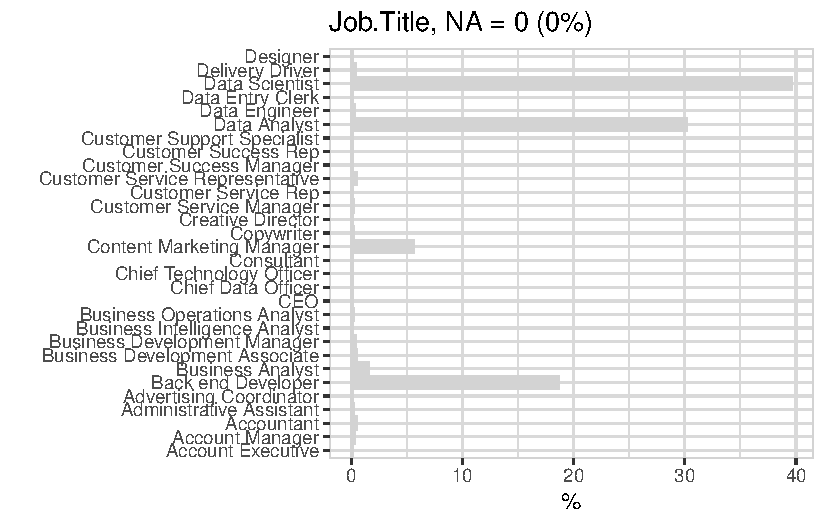
\includegraphics{main_doc_files/figure-pdf/unnamed-chunk-7-1.pdf}

}

\end{figure}

Altersverteilung:

\begin{Shaded}
\begin{Highlighting}[]
\FunctionTok{ggplot}\NormalTok{(salary, }\FunctionTok{aes}\NormalTok{(}\AttributeTok{x =}\NormalTok{ Age)) }\SpecialCharTok{+}
  \FunctionTok{geom\_histogram}\NormalTok{(}\AttributeTok{binwidth =} \DecValTok{5}\NormalTok{, }\AttributeTok{fill =} \StringTok{"skyblue"}\NormalTok{, }\AttributeTok{color =} \StringTok{"black"}\NormalTok{, }\AttributeTok{alpha =} \FloatTok{0.8}\NormalTok{) }\SpecialCharTok{+}
  \FunctionTok{labs}\NormalTok{(}\AttributeTok{title =} \StringTok{"Age Distribution"}\NormalTok{,}
       \AttributeTok{x =} \StringTok{"Age"}\NormalTok{,}
       \AttributeTok{y =} \StringTok{"Frequency"}\NormalTok{)}
\end{Highlighting}
\end{Shaded}

\begin{figure}[H]

{\centering 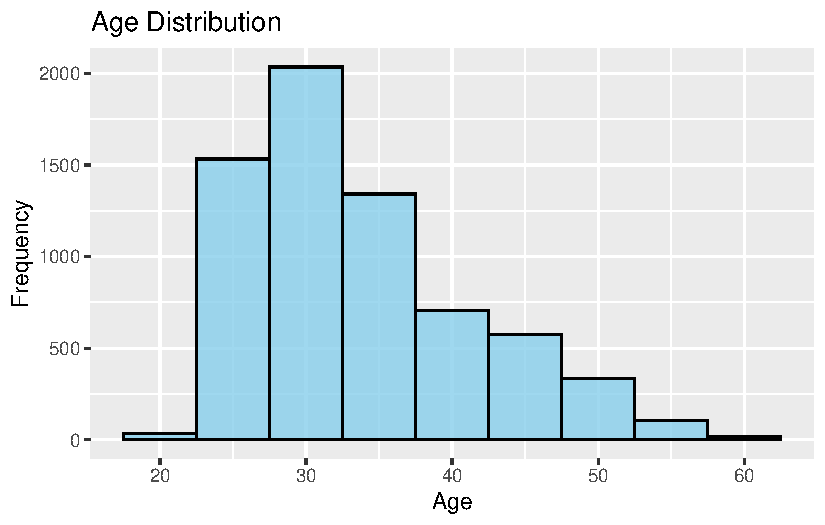
\includegraphics{main_doc_files/figure-pdf/unnamed-chunk-8-1.pdf}

}

\end{figure}

Verteilung des Bildungsniveaus:

Zunächst wird eine Farbpalette mit verschiedenen Farben definiert.
Anschließend wird ein Balkendiagramm erstellt, wobei unterschiedliche
Farben für jede Balkenstange verwendet werden, basierend auf dem
Bildungsniveau.

\begin{Shaded}
\begin{Highlighting}[]
\NormalTok{my\_colors }\OtherTok{\textless{}{-}} \FunctionTok{c}\NormalTok{(}\StringTok{"skyblue"}\NormalTok{, }\StringTok{"lightgreen"}\NormalTok{, }\StringTok{"salmon"}\NormalTok{, }\StringTok{"gold"}\NormalTok{) }
\FunctionTok{ggplot}\NormalTok{(salary, }\FunctionTok{aes}\NormalTok{(}\AttributeTok{x =} \FunctionTok{factor}\NormalTok{(}\StringTok{\textasciigrave{}}\AttributeTok{Education.Level}\StringTok{\textasciigrave{}}\NormalTok{))) }\SpecialCharTok{+}
  \FunctionTok{geom\_bar}\NormalTok{(}\AttributeTok{fill =}\NormalTok{ my\_colors, }\AttributeTok{color =} \StringTok{"black"}\NormalTok{) }\SpecialCharTok{+}
  \FunctionTok{labs}\NormalTok{(}\AttributeTok{title =} \StringTok{"Verteilung des Bildungsniveaus"}\NormalTok{,}
       \AttributeTok{x =} \StringTok{"Bildungsniveau"}\NormalTok{,}
       \AttributeTok{y =} \StringTok{"Anzahl"}\NormalTok{) }\SpecialCharTok{+}
  \FunctionTok{theme}\NormalTok{(}\AttributeTok{axis.text.x =} \FunctionTok{element\_text}\NormalTok{(}\AttributeTok{angle =} \DecValTok{45}\NormalTok{, }\AttributeTok{hjust =} \DecValTok{1}\NormalTok{))}
\end{Highlighting}
\end{Shaded}

\begin{figure}[H]

{\centering 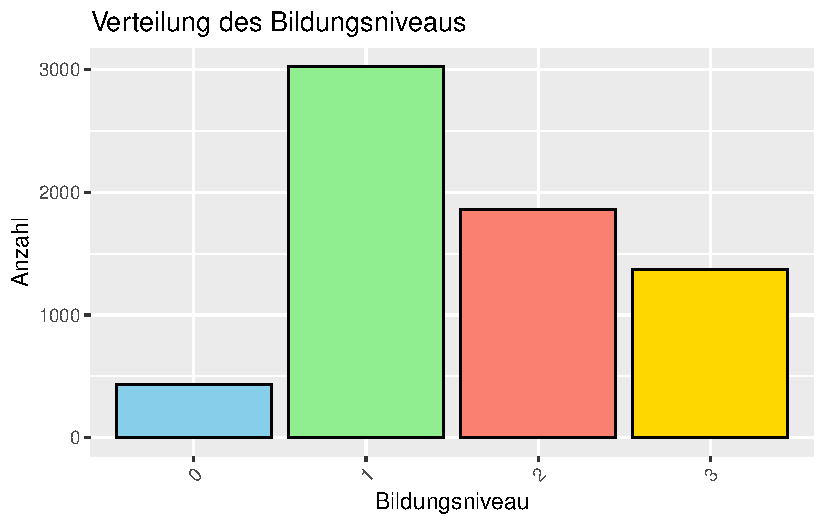
\includegraphics{main_doc_files/figure-pdf/unnamed-chunk-9-1.pdf}

}

\end{figure}

Verteilung der Arbeitserfahrung in Jahren:

Ab diesem Punkt wurde teilweise das Paket ``Viridis'' für die farbliche
Darstellung verwendet, um eine Alternative zur manuellen Deklaration der
Farben aufzuzeigen.

\begin{Shaded}
\begin{Highlighting}[]
\FunctionTok{ggplot}\NormalTok{(salary, }\FunctionTok{aes}\NormalTok{(}\AttributeTok{x =} \StringTok{\textasciigrave{}}\AttributeTok{Years.Of.Experience}\StringTok{\textasciigrave{}}\NormalTok{)) }\SpecialCharTok{+}
  \FunctionTok{geom\_histogram}\NormalTok{(}\AttributeTok{binwidth =} \DecValTok{5}\NormalTok{, }\AttributeTok{fill =} \FunctionTok{viridis}\NormalTok{(}\DecValTok{8}\NormalTok{), }\AttributeTok{color =} \StringTok{"black"}\NormalTok{) }\SpecialCharTok{+}
  \FunctionTok{labs}\NormalTok{(}\AttributeTok{title =} \StringTok{"Verteilung der Berufserfahrung"}\NormalTok{,}
       \AttributeTok{x =} \StringTok{"Jahre an Erfahrung"}\NormalTok{,}
       \AttributeTok{y =} \StringTok{"Häufigkeit"}\NormalTok{) }\SpecialCharTok{+}
  \FunctionTok{theme\_minimal}\NormalTok{()}
\end{Highlighting}
\end{Shaded}

\begin{figure}[H]

{\centering 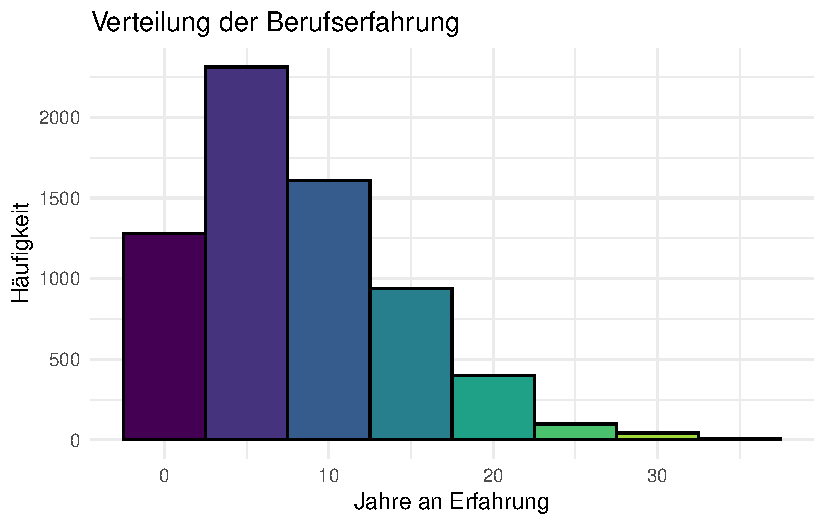
\includegraphics{main_doc_files/figure-pdf/unnamed-chunk-10-1.pdf}

}

\end{figure}

Verteilung der Geschlechter:

\begin{Shaded}
\begin{Highlighting}[]
\FunctionTok{ggplot}\NormalTok{(salary, }\FunctionTok{aes}\NormalTok{(}\AttributeTok{x=}\NormalTok{Gender)) }\SpecialCharTok{+}
  \FunctionTok{geom\_bar}\NormalTok{(}\AttributeTok{fill=}\FunctionTok{viridis}\NormalTok{(}\DecValTok{2}\NormalTok{)) }\SpecialCharTok{+}
  \FunctionTok{ggtitle}\NormalTok{(}\StringTok{"Gender Distribution"}\NormalTok{) }\SpecialCharTok{+}
  \FunctionTok{xlab}\NormalTok{(}\StringTok{"Gender"}\NormalTok{) }\SpecialCharTok{+}
  \FunctionTok{ylab}\NormalTok{(}\StringTok{"Count"}\NormalTok{) }\SpecialCharTok{+}
  \FunctionTok{theme}\NormalTok{(}\AttributeTok{plot.title =} \FunctionTok{element\_text}\NormalTok{(}\AttributeTok{hjust =} \FloatTok{0.5}\NormalTok{))}
\end{Highlighting}
\end{Shaded}

\begin{figure}[H]

{\centering 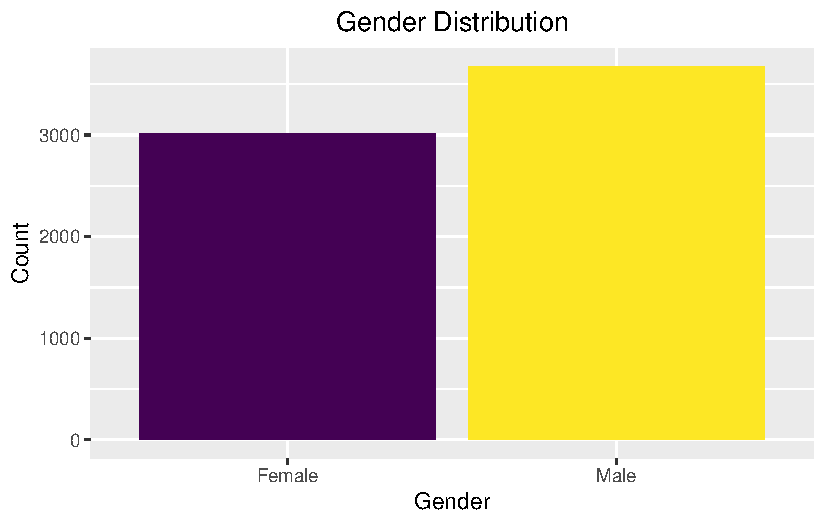
\includegraphics{main_doc_files/figure-pdf/unnamed-chunk-11-1.pdf}

}

\end{figure}

Verteilung der Länder:

(Alternative Nutzung des Farbschemas):

\begin{Shaded}
\begin{Highlighting}[]
\FunctionTok{ggplot}\NormalTok{(salary, }\FunctionTok{aes}\NormalTok{(}\AttributeTok{x =}\NormalTok{ Country, }\AttributeTok{fill =}\NormalTok{ Country)) }\SpecialCharTok{+}
  \FunctionTok{geom\_bar}\NormalTok{() }\SpecialCharTok{+}
  \FunctionTok{scale\_fill\_viridis}\NormalTok{(}\AttributeTok{discrete =} \ConstantTok{TRUE}\NormalTok{) }\SpecialCharTok{+}
  \FunctionTok{ggtitle}\NormalTok{(}\StringTok{"Country Distribution"}\NormalTok{) }\SpecialCharTok{+}
  \FunctionTok{xlab}\NormalTok{(}\StringTok{"Country"}\NormalTok{) }\SpecialCharTok{+}
  \FunctionTok{ylab}\NormalTok{(}\StringTok{"Count"}\NormalTok{) }\SpecialCharTok{+}
  \FunctionTok{theme}\NormalTok{(}\AttributeTok{axis.text.x =} \FunctionTok{element\_text}\NormalTok{(}\AttributeTok{angle =} \DecValTok{45}\NormalTok{, }\AttributeTok{hjust =} \DecValTok{1}\NormalTok{))}
\end{Highlighting}
\end{Shaded}

\begin{figure}[H]

{\centering 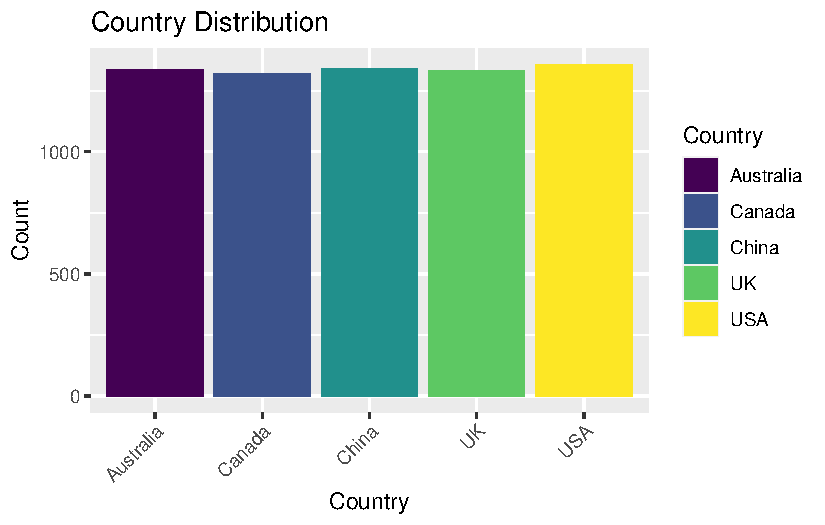
\includegraphics{main_doc_files/figure-pdf/unnamed-chunk-12-1.pdf}

}

\end{figure}

Verteilung der Ethnizitäten:

\begin{Shaded}
\begin{Highlighting}[]
\FunctionTok{ggplot}\NormalTok{(salary, }\FunctionTok{aes}\NormalTok{(}\AttributeTok{x =}\NormalTok{ Race, }\AttributeTok{fill =}\NormalTok{ Race)) }\SpecialCharTok{+}
  \FunctionTok{geom\_bar}\NormalTok{() }\SpecialCharTok{+}
  \FunctionTok{scale\_fill\_viridis}\NormalTok{(}\AttributeTok{discrete =} \ConstantTok{TRUE}\NormalTok{) }\SpecialCharTok{+}
  \FunctionTok{ggtitle}\NormalTok{(}\StringTok{"Race Distribution"}\NormalTok{) }\SpecialCharTok{+}
  \FunctionTok{xlab}\NormalTok{(}\StringTok{"Race"}\NormalTok{) }\SpecialCharTok{+}
  \FunctionTok{ylab}\NormalTok{(}\StringTok{"Count"}\NormalTok{) }\SpecialCharTok{+}
  \FunctionTok{theme}\NormalTok{(}\AttributeTok{axis.text.x =} \FunctionTok{element\_text}\NormalTok{(}\AttributeTok{angle =} \DecValTok{45}\NormalTok{, }\AttributeTok{hjust =} \DecValTok{1}\NormalTok{))}
\end{Highlighting}
\end{Shaded}

\begin{figure}[H]

{\centering 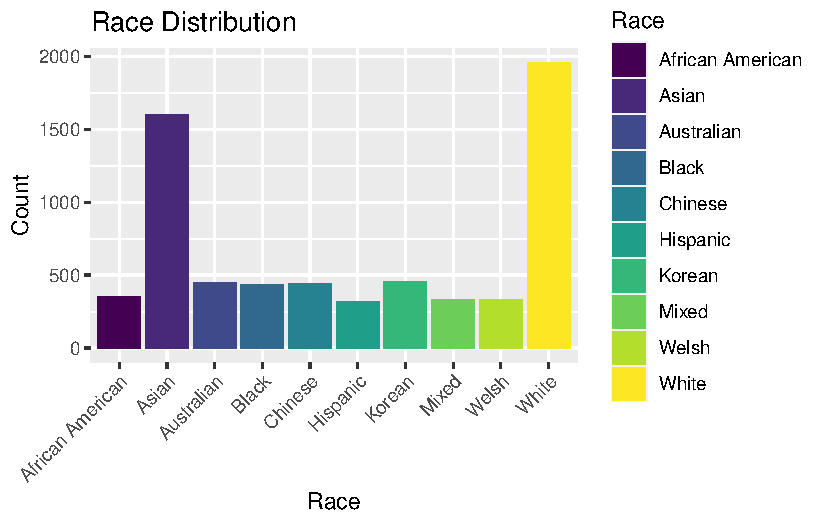
\includegraphics{main_doc_files/figure-pdf/unnamed-chunk-13-1.pdf}

}

\end{figure}

Verteilung der 10 häufigsten Job Titel:

\begin{Shaded}
\begin{Highlighting}[]
\CommentTok{\# Die Top 10 Jobtitel auswählen}
\NormalTok{top\_job\_titles }\OtherTok{\textless{}{-}} \FunctionTok{names}\NormalTok{(}\FunctionTok{sort}\NormalTok{(}\FunctionTok{table}\NormalTok{(salary}\SpecialCharTok{$}\NormalTok{Job.Title), }\AttributeTok{decreasing =} \ConstantTok{TRUE}\NormalTok{)[}\DecValTok{1}\SpecialCharTok{:}\DecValTok{10}\NormalTok{])}

\CommentTok{\# Zufällige Farben für jeden Jobtitel generieren}
\NormalTok{job\_colors }\OtherTok{\textless{}{-}} \FunctionTok{rainbow}\NormalTok{(}\FunctionTok{length}\NormalTok{(top\_job\_titles))}

\CommentTok{\# Daten filtern und ggplot erstellen}
\FunctionTok{ggplot}\NormalTok{(salary[salary}\SpecialCharTok{$}\NormalTok{Job.Title }\SpecialCharTok{\%in\%}\NormalTok{ top\_job\_titles, ], }\FunctionTok{aes}\NormalTok{(}\AttributeTok{x =} \FunctionTok{factor}\NormalTok{(Job.Title, }\AttributeTok{levels =}\NormalTok{ top\_job\_titles), }\AttributeTok{fill =} \FunctionTok{factor}\NormalTok{(Job.Title))) }\SpecialCharTok{+}
  \FunctionTok{geom\_bar}\NormalTok{(}\AttributeTok{fill=}\FunctionTok{viridis}\NormalTok{(}\DecValTok{10}\NormalTok{)) }\SpecialCharTok{+}
  \FunctionTok{scale\_fill\_manual}\NormalTok{(}\AttributeTok{values =}\NormalTok{ job\_colors) }\SpecialCharTok{+}
  \FunctionTok{labs}\NormalTok{(}\AttributeTok{title =} \StringTok{"Top 10 Job Titles Distribution"}\NormalTok{,}
       \AttributeTok{x =} \StringTok{"Job Title"}\NormalTok{,}
       \AttributeTok{y =} \StringTok{"Count"}\NormalTok{) }\SpecialCharTok{+}
  \FunctionTok{theme}\NormalTok{(}\AttributeTok{axis.text.x =} \FunctionTok{element\_text}\NormalTok{(}\AttributeTok{angle =} \DecValTok{45}\NormalTok{, }\AttributeTok{hjust =} \DecValTok{1}\NormalTok{))}
\end{Highlighting}
\end{Shaded}

\begin{figure}[H]

{\centering 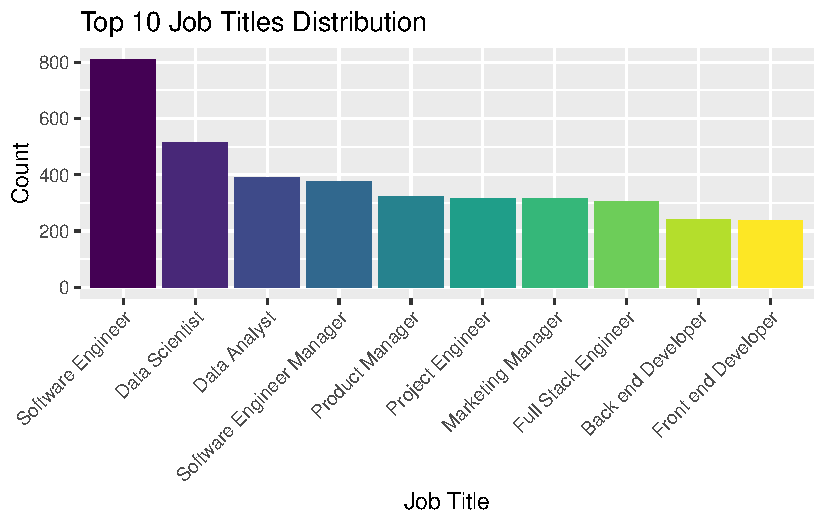
\includegraphics{main_doc_files/figure-pdf/unnamed-chunk-14-1.pdf}

}

\end{figure}

\hypertarget{grundlegende-statistische-merkmale-des-datensatzes}{%
\subsection{2.2 Grundlegende Statistische Merkmale des
Datensatzes}\label{grundlegende-statistische-merkmale-des-datensatzes}}

Zunächst wird mithilfe der Funktion ``summary()'' ein allgemeiner
Überblick über die wichtigsten charakteristischen Merkmale der einzelnen
Spalten gegeben.

\begin{Shaded}
\begin{Highlighting}[]
\FunctionTok{summary}\NormalTok{(salary)}
\end{Highlighting}
\end{Shaded}

\begin{verbatim}
      Age           Gender          Education.Level  Job.Title        
 Min.   :21.00   Length:6684        Min.   :0.000   Length:6684       
 1st Qu.:28.00   Class :character   1st Qu.:1.000   Class :character  
 Median :32.00   Mode  :character   Median :1.000   Mode  :character  
 Mean   :33.61                      Mean   :1.622                     
 3rd Qu.:38.00                      3rd Qu.:2.000                     
 Max.   :62.00                      Max.   :3.000                     
 Years.Of.Experience     Salary         Country              Race          
 Min.   : 0.000      Min.   :   350   Length:6684        Length:6684       
 1st Qu.: 3.000      1st Qu.: 70000   Class :character   Class :character  
 Median : 7.000      Median :115000   Mode  :character   Mode  :character  
 Mean   : 8.078      Mean   :115307                                        
 3rd Qu.:12.000      3rd Qu.:160000                                        
 Max.   :34.000      Max.   :250000                                        
     Senior      
 Min.   :0.0000  
 1st Qu.:0.0000  
 Median :0.0000  
 Mean   :0.1435  
 3rd Qu.:0.0000  
 Max.   :1.0000  
\end{verbatim}

In einer ersten Analyse zeigt sich, dass der durchschnittliche
Alterswert im Datensatz bei 32 Jahren liegt. Die Altersspanne erstreckt
sich dabei von 21 bis 62 Jahren. Bezüglich des ``Education-Level''
variieren die Werte zwischen 1, 2 und 3, wobei der Durchschnitt bei 1
liegt. In Bezug auf die Berufserfahrung (``Years of Experience'')
reichen die Werte von 0 bis zu 34 Jahren, wobei der Median hier bei 7
liegt. Bei Auswertung der Gehaltsdaten (``Salary'') ergibt sich, dass
das Mindestgehalt bei 350 Dollar, das Höchstgehalt bei 250.000 Dollar
und der Median bei 115.000 Dollar liegt.

\hypertarget{umstrukturierung-des-datensatzes-fuxfcr-eine-verbesserte-visualisierung}{%
\section{3. Umstrukturierung des Datensatzes für eine verbesserte
Visualisierung}\label{umstrukturierung-des-datensatzes-fuxfcr-eine-verbesserte-visualisierung}}

Im folgenden wird der Datensatz temporär umstrukturiert, um den
Datensatz besser analysieren und visualieren zu können.

Ein neuer Wert Namens ``Value'' wird erschaffen.

\begin{Shaded}
\begin{Highlighting}[]
\NormalTok{Salary\_long }\OtherTok{\textless{}{-}} \FunctionTok{select}\NormalTok{(salary, }\SpecialCharTok{{-}}\NormalTok{Job.Title, }\SpecialCharTok{{-}}\NormalTok{Gender, }\SpecialCharTok{{-}}\NormalTok{Race, }\SpecialCharTok{{-}}\NormalTok{Country, }\SpecialCharTok{{-}}\NormalTok{Senior)}
\NormalTok{Salary\_long }\OtherTok{\textless{}{-}} \FunctionTok{pivot\_longer}\NormalTok{(Salary\_long, }\FunctionTok{colnames}\NormalTok{(Salary\_long))}
\NormalTok{Salary }\OtherTok{\textless{}{-}} \FunctionTok{as.data.frame}\NormalTok{(Salary\_long) }
\FunctionTok{head}\NormalTok{(Salary\_long)}
\end{Highlighting}
\end{Shaded}

\begin{verbatim}
# A tibble: 6 x 2
  name                value
  <chr>               <dbl>
1 Age                    32
2 Education.Level         1
3 Years.Of.Experience     5
4 Salary              90000
5 Age                    28
6 Education.Level         2
\end{verbatim}

In diesem Codeabschnitt werden sämtliche Spalten, die keine numerischen
Merkmale repräsentieren, entfernt. Der verbleibende Datensatz wird
anschließend von einem breiten Format in ein längeres umgewandelt. Diese
Transformation ermöglicht eine effizientere Analyse und Visualisierung
der numerischen Daten, indem sie sie in einer strukturierteren und
leichter interpretierbaren Form darstellt.

Hier kann man folgende Dinge erkennen:

\begin{itemize}
\item
  Age, Years of Experience und Education Level sind Linksschief und
  haben ggf. Bedarf einer Transformation für ML-Modelle
\item
  Age und Years of Experience haben Extrempunkte im oberen Wertebereich,
  während Salary einer gleichmäßigen Verteilung folgt
\end{itemize}

Aufgrund der sorgfältigen Strukturierung der Daten, scheinen sie auf den
ersten Blick gut für eine umfassende explorative Analyse geeignet zu
sein.

\hypertarget{kategorisierung-von-gehalt}{%
\subsection{3.1 Kategorisierung von
Gehalt}\label{kategorisierung-von-gehalt}}

Zunächst werden die Daten aus dem Ausgangsdatensatz in einen finalen
Datensatz ``salary\_final'' geschrieben.

\begin{Shaded}
\begin{Highlighting}[]
\NormalTok{salary\_final }\OtherTok{\textless{}{-}}\NormalTok{ salary}
\end{Highlighting}
\end{Shaded}

Durch den Befehl ``hist()'' wird ein Histogramm erstellt. Es ermöglicht
eine visuelle Darstellung der Häufigkeitsverteilung dieser Gehaltsdaten,
indem es zeigt, wie oft bestimmte Gehaltsbereiche vorkommen.

Verteilung des Gehalts:

\begin{Shaded}
\begin{Highlighting}[]
\FunctionTok{ggplot}\NormalTok{(salary, }\FunctionTok{aes}\NormalTok{(}\AttributeTok{x =}\NormalTok{ Salary)) }\SpecialCharTok{+}
  \FunctionTok{geom\_histogram}\NormalTok{(}\AttributeTok{binwidth =} \DecValTok{10000}\NormalTok{, }\AttributeTok{fill =} \FunctionTok{viridis}\NormalTok{(}\DecValTok{26}\NormalTok{), }\AttributeTok{color =} \StringTok{"black"}\NormalTok{) }\SpecialCharTok{+}
  \FunctionTok{labs}\NormalTok{(}\AttributeTok{title =} \StringTok{"Gehaltsverteilung"}\NormalTok{,}
       \AttributeTok{x =} \StringTok{"Gehalt"}\NormalTok{,}
       \AttributeTok{y =} \StringTok{"Häufigkeit"}\NormalTok{) }\SpecialCharTok{+}
  \FunctionTok{scale\_y\_continuous}\NormalTok{(}\AttributeTok{labels =}\NormalTok{ scales}\SpecialCharTok{::}\NormalTok{comma) }\SpecialCharTok{+}
  \FunctionTok{scale\_x\_continuous}\NormalTok{(}\AttributeTok{labels =}\NormalTok{ scales}\SpecialCharTok{::}\NormalTok{comma) }\SpecialCharTok{+}
  \FunctionTok{theme\_minimal}\NormalTok{()}
\end{Highlighting}
\end{Shaded}

\begin{figure}[H]

{\centering 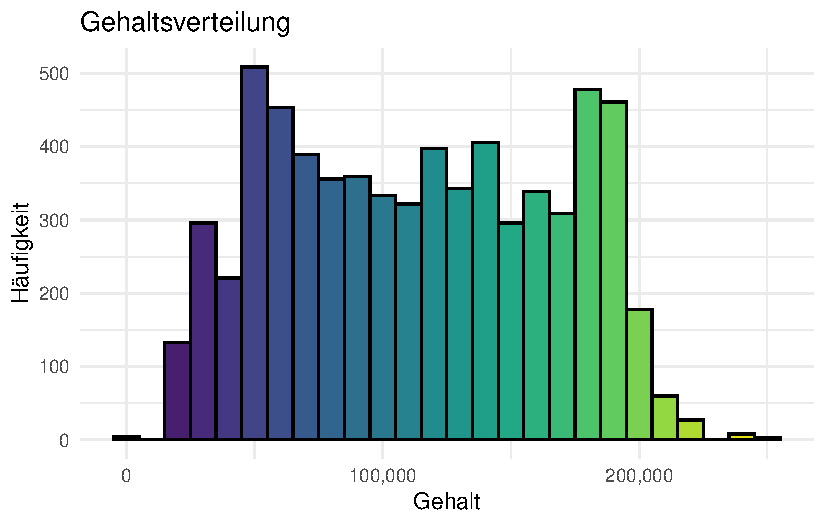
\includegraphics{main_doc_files/figure-pdf/unnamed-chunk-18-1.pdf}

}

\end{figure}

Im weiteren Verlauf wird eine neue Spalte namens ``SalaryKat'' erstellt,
die kategorische Werte basierend auf den Gehältern enthält. Darauf
aufbauend wird ein Balkendiagramm für die 5 Gehaltskategorien erstellt.
Diese visuelle Darstellung ermöglicht eine effektive Einsicht in die
Verteilung der Gehälter und erleichtert die Interpretation der Daten in
übersichtlicher Form.

\begin{Shaded}
\begin{Highlighting}[]
\NormalTok{salary\_final}\SpecialCharTok{$}\NormalTok{SalaryKat }\OtherTok{\textless{}{-}} \FunctionTok{cut}\NormalTok{(salary\_final}\SpecialCharTok{$}\NormalTok{Salary, }
                  \AttributeTok{breaks =} \FunctionTok{c}\NormalTok{(}\SpecialCharTok{{-}}\ConstantTok{Inf}\NormalTok{, }\DecValTok{50000}\NormalTok{, }\DecValTok{100000}\NormalTok{, }\DecValTok{150000}\NormalTok{, }\DecValTok{200000}\NormalTok{, }\DecValTok{250000}\NormalTok{, }\ConstantTok{Inf}\NormalTok{),                      }\AttributeTok{labels =} \FunctionTok{c}\NormalTok{(}\StringTok{"50000"}\NormalTok{, }\StringTok{"100000"}\NormalTok{, }\StringTok{"150000"}\NormalTok{, }\StringTok{"200000"}\NormalTok{,}\StringTok{"250000"}\NormalTok{, }\StringTok{"300000"}\NormalTok{))}
\end{Highlighting}
\end{Shaded}

\begin{Shaded}
\begin{Highlighting}[]
\FunctionTok{ggplot}\NormalTok{(salary\_final, }\FunctionTok{aes}\NormalTok{(}\AttributeTok{x =}\NormalTok{ SalaryKat, }\AttributeTok{fill =}\NormalTok{ SalaryKat)) }\SpecialCharTok{+}
  \FunctionTok{geom\_bar}\NormalTok{() }\SpecialCharTok{+}
  \FunctionTok{scale\_fill\_viridis}\NormalTok{(}\AttributeTok{discrete =} \ConstantTok{TRUE}\NormalTok{) }\SpecialCharTok{+}
  \FunctionTok{ggtitle}\NormalTok{(}\StringTok{"Verteilung der Gehaltskategorien"}\NormalTok{) }\SpecialCharTok{+}
  \FunctionTok{xlab}\NormalTok{(}\StringTok{"Gehaltskategorie"}\NormalTok{) }\SpecialCharTok{+}
  \FunctionTok{ylab}\NormalTok{(}\StringTok{"Anzahl"}\NormalTok{) }\SpecialCharTok{+}
  \FunctionTok{theme}\NormalTok{(}\AttributeTok{axis.text.x =} \FunctionTok{element\_text}\NormalTok{(}\AttributeTok{angle =} \DecValTok{45}\NormalTok{, }\AttributeTok{hjust =} \DecValTok{1}\NormalTok{))}
\end{Highlighting}
\end{Shaded}

\begin{figure}[H]

{\centering 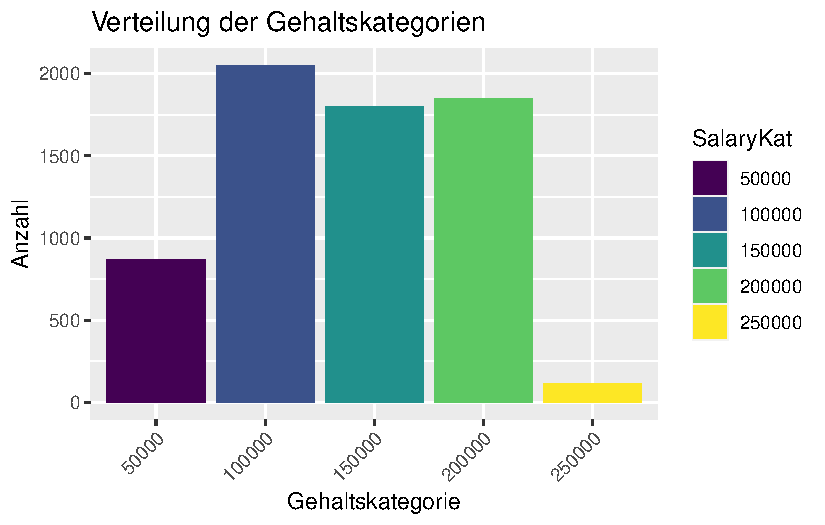
\includegraphics{main_doc_files/figure-pdf/unnamed-chunk-20-1.pdf}

}

\end{figure}

Die Analyse der erstellten Gehaltskategorie zeigt, dass die Kategorie
mit einem Gehalt von 100.000 am häufigsten vertreten ist.

\hypertarget{korrelationen}{%
\subsection{3.2 Korrelationen}\label{korrelationen}}

Im weiteren Verlauf erfolgt die Berechnung der Korrelationen zwischen
den verschiedenen Spalten.

Diese Vorgehensweise ermöglicht es, die Stärke und Richtung des
Zusammenhangs zwischen zwei Variablen zu quantifizieren. Die Anwendung
von Korrelationsanalysen spielt eine entscheidende Rolle bei der
Modellvalidierung, da sie dabei hilft, potenzielle Probleme wie
beispielsweise Multikollinearität zu identifizieren.

Die folgenden Korrelationen werden nun berechnet:

\begin{Shaded}
\begin{Highlighting}[]
\CommentTok{\# Korrelation zwischen Salary und Years.Of.Experience berechnen}
\NormalTok{correlation\_salary\_experience }\OtherTok{\textless{}{-}} \FunctionTok{cor}\NormalTok{(salary\_final}\SpecialCharTok{$}\NormalTok{Salary, salary\_final}\SpecialCharTok{$}\NormalTok{Years.Of.Experience)}

\CommentTok{\# Ausgabe des Ergebnisses}
\FunctionTok{cat}\NormalTok{(}\StringTok{"Die Korrelation zwischen Salary und Years.Of.Experience ist:"}\NormalTok{, correlation\_salary\_experience, }\StringTok{"}\SpecialCharTok{\textbackslash{}n}\StringTok{"}\NormalTok{)}
\end{Highlighting}
\end{Shaded}

\begin{verbatim}
Die Korrelation zwischen Salary und Years.Of.Experience ist: 0.8109416 
\end{verbatim}

\begin{Shaded}
\begin{Highlighting}[]
\CommentTok{\# Korrelation zwischen Salary und Age berechnen}
\NormalTok{correlation\_salary\_age }\OtherTok{\textless{}{-}} \FunctionTok{cor}\NormalTok{(salary\_final}\SpecialCharTok{$}\NormalTok{Salary, salary\_final}\SpecialCharTok{$}\NormalTok{Age, }\AttributeTok{use =} \StringTok{"complete.obs"}\NormalTok{)}

\CommentTok{\# Ausgabe des Ergebnisses}
\FunctionTok{cat}\NormalTok{(}\StringTok{"Die Korrelation zwischen Salary und Age ist:"}\NormalTok{, correlation\_salary\_age, }\StringTok{"}\SpecialCharTok{\textbackslash{}n}\StringTok{"}\NormalTok{)}
\end{Highlighting}
\end{Shaded}

\begin{verbatim}
Die Korrelation zwischen Salary und Age ist: 0.7283429 
\end{verbatim}

\begin{Shaded}
\begin{Highlighting}[]
\CommentTok{\# Korrelation zwischen Years.Of.Experience und Age berechnen}
\NormalTok{correlation\_experience\_age }\OtherTok{\textless{}{-}} \FunctionTok{cor}\NormalTok{(salary\_final}\SpecialCharTok{$}\NormalTok{Years.Of.Experience, salary\_final}\SpecialCharTok{$}\NormalTok{Age, }\AttributeTok{use =} \StringTok{"complete.obs"}\NormalTok{)}

\CommentTok{\# Ausgabe des Ergebnisses}
\FunctionTok{cat}\NormalTok{(}\StringTok{"Die Korrelation zwischen Years.Of.Experience und Age ist:"}\NormalTok{, correlation\_experience\_age, }\StringTok{"}\SpecialCharTok{\textbackslash{}n}\StringTok{"}\NormalTok{)}
\end{Highlighting}
\end{Shaded}

\begin{verbatim}
Die Korrelation zwischen Years.Of.Experience und Age ist: 0.9376094 
\end{verbatim}

\begin{Shaded}
\begin{Highlighting}[]
\CommentTok{\# Korrelation zwischen Seniority und Years.Of.Experience berechnen}
\NormalTok{correlation\_seniority\_experience }\OtherTok{\textless{}{-}} \FunctionTok{cor}\NormalTok{(salary\_final}\SpecialCharTok{$}\NormalTok{Senior, salary\_final}\SpecialCharTok{$}\NormalTok{Years.Of.Experience, }\AttributeTok{use =} \StringTok{"complete.obs"}\NormalTok{)}

\CommentTok{\# Ausgabe des Ergebnisses}
\FunctionTok{cat}\NormalTok{(}\StringTok{"Die Korrelation zwischen Seniority und Years.Of.Experience ist:"}\NormalTok{, correlation\_seniority\_experience, }\StringTok{"}\SpecialCharTok{\textbackslash{}n}\StringTok{"}\NormalTok{)}
\end{Highlighting}
\end{Shaded}

\begin{verbatim}
Die Korrelation zwischen Seniority und Years.Of.Experience ist: 0.3178772 
\end{verbatim}

Die Ergebnisse der Korrelationen:

\begin{itemize}
\item
  Von salary und years.of.experience ist es 0.81.
\item
  Von Salary und Age ist es 0.73
\item
  von Age und Years of Experience st es 0.93.
\end{itemize}

Nun stellt sich folgende Frage:

Wie entsteht bei den Werten so ein starker Unterschied, im Vergleich zu
Salary, obwohl eine so hohe Korrelation zueinander besteht?

Lösungsansätze:

Verteilung der Daten: Es ist möglich, dass die Verteilung der Daten in
den Variablen ``Age'' und ``Years.Of.Experience'' anders ist als in der
Variable ``Salary''. Wenn die Daten in ``Age'' und
``Years.Of.Experience'' breiter gestreut sind, kann dies zu einer
geringeren Korrelation führen, selbst wenn eine starke lineare Beziehung
besteht.

Nicht-lineare Beziehung: Die Korrelation misst nur lineare Beziehungen.
Wenn die Beziehung zwischen ``Age'' und ``Years.Of.Experience'' nicht
linear ist, könnte dies zu einem niedrigeren Korrelationswert führen.

Ausreißer: Das Vorhandensein von Ausreißern kann die Korrelation
beeinflussen. Wenn es Ausreißer in einer der Variablen gibt, kann dies
den Korrelationswert beeinträchtigen.

Stichprobengröße: Bei kleineren Stichproben können Korrelationswerte
instabiler sein.

\hypertarget{tests-fuxfcr-die-thesen}{%
\section{4. Tests für die Thesen}\label{tests-fuxfcr-die-thesen}}

Im weiteren Verlauf werden anhand der vorliegenden Daten verschiedene
Tests durchgeführt, um Aussagen für die aufgestellten Thesen
herauszufiltern. Dieser Prozess wird sowohl durch die Visualisierung der
Beziehungen zwischen den verschiedenen Spalten als auch durch die
Berechnung von Korrelationen unterstützt. Die Kombination dieser
Methoden ermöglicht eine umfassende Analyse, die dazu beiträgt, Muster,
Trends und potenzielle Zusammenhänge zwischen den betrachteten Variablen
zu erkennen.

\hypertarget{korrelationen-1}{%
\subsection{4.1 Korrelationen}\label{korrelationen-1}}

Das Ergebnis dieses Codechunks ist eine Darstellung der
Korrelationsmatrix:

\begin{Shaded}
\begin{Highlighting}[]
\NormalTok{correlations }\OtherTok{\textless{}{-}} \FunctionTok{cor}\NormalTok{(salary\_final[, }\FunctionTok{c}\NormalTok{(}\StringTok{"Age"}\NormalTok{, }\StringTok{"Education.Level"}\NormalTok{, }\StringTok{"Years.Of.Experience"}\NormalTok{, }\StringTok{"Salary"}\NormalTok{)])}

\FunctionTok{print}\NormalTok{(correlations)}
\end{Highlighting}
\end{Shaded}

\begin{verbatim}
                          Age Education.Level Years.Of.Experience    Salary
Age                 1.0000000       0.5963804           0.9376094 0.7283429
Education.Level     0.5963804       1.0000000           0.6131650 0.6454436
Years.Of.Experience 0.9376094       0.6131650           1.0000000 0.8109416
Salary              0.7283429       0.6454436           0.8109416 1.0000000
\end{verbatim}

Erkennbar ist eine starke Korrelation zwischen dem Alter und den ``Years
of Experience''. Des Weiteren besteht ebenfalls eine ausgeprägte
Korrelation zwischen den Years of Experience und dem endgültigen Gehalt.
Hingegen liegt die Korrelation zwischen dem Alter und dem Bildungsniveau
mit einem Wert von ungefähr 0,6 nicht ganz so stark vor.

\begin{Shaded}
\begin{Highlighting}[]
\NormalTok{filtered\_data\_numeric }\OtherTok{\textless{}{-}} \FunctionTok{select}\NormalTok{(salary, Salary, Age, Years.Of.Experience, Education.Level)}
\FunctionTok{glimpse}\NormalTok{(filtered\_data\_numeric)}
\end{Highlighting}
\end{Shaded}

\begin{verbatim}
Rows: 6,684
Columns: 4
$ Salary              <dbl> 90000, 65000, 150000, 60000, 200000, 55000, 120000~
$ Age                 <dbl> 32, 28, 45, 36, 52, 29, 42, 31, 26, 38, 29, 48, 35~
$ Years.Of.Experience <dbl> 5, 3, 15, 7, 20, 2, 12, 4, 1, 10, 3, 18, 6, 14, 2,~
$ Education.Level     <dbl> 1, 2, 3, 1, 2, 1, 2, 1, 1, 3, 2, 1, 1, 2, 1, 1, 2,~
\end{verbatim}

\begin{Shaded}
\begin{Highlighting}[]
\FunctionTok{cor}\NormalTok{(filtered\_data\_numeric)}
\end{Highlighting}
\end{Shaded}

\begin{verbatim}
                       Salary       Age Years.Of.Experience Education.Level
Salary              1.0000000 0.7283429           0.8109416       0.6454436
Age                 0.7283429 1.0000000           0.9376094       0.5963804
Years.Of.Experience 0.8109416 0.9376094           1.0000000       0.6131650
Education.Level     0.6454436 0.5963804           0.6131650       1.0000000
\end{verbatim}

Nun wird der Korrelationsplot erstellt.

\begin{Shaded}
\begin{Highlighting}[]
\FunctionTok{corrplot}\NormalTok{(}\FunctionTok{cor}\NormalTok{(filtered\_data\_numeric), }\AttributeTok{method =} \StringTok{"ellipse"}\NormalTok{, }\AttributeTok{col =} \FunctionTok{viridis}\NormalTok{(}\DecValTok{200}\NormalTok{))}
\end{Highlighting}
\end{Shaded}

\begin{figure}[H]

{\centering 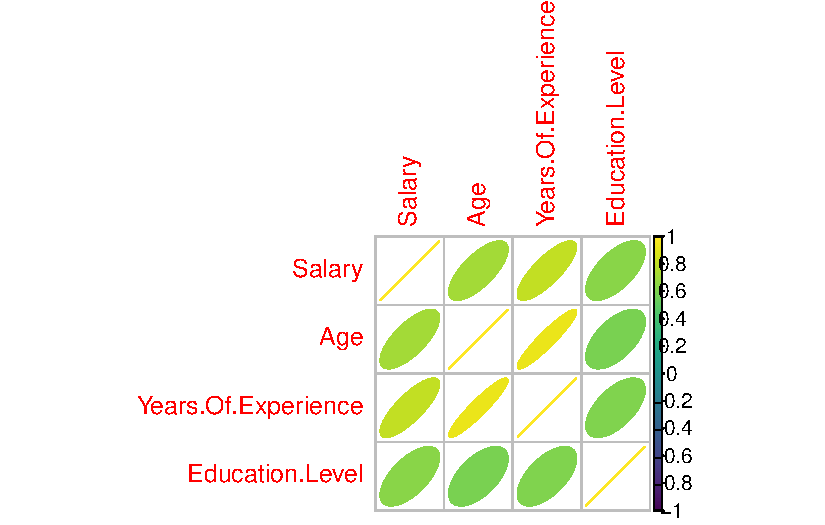
\includegraphics{main_doc_files/figure-pdf/unnamed-chunk-27-1.pdf}

}

\end{figure}

\hypertarget{streudiagramme}{%
\subsection{4.2 Streudiagramme}\label{streudiagramme}}

\begin{Shaded}
\begin{Highlighting}[]
\FunctionTok{ggplot}\NormalTok{(salary\_final, }\FunctionTok{aes}\NormalTok{(}\AttributeTok{x =}\NormalTok{ Years.Of.Experience, }\AttributeTok{y =}\NormalTok{ Salary)) }\SpecialCharTok{+}
  \FunctionTok{geom\_point}\NormalTok{(}\AttributeTok{color =} \FunctionTok{viridis}\NormalTok{(}\DecValTok{2}\NormalTok{)[}\DecValTok{1}\NormalTok{], }\AttributeTok{size =} \DecValTok{3}\NormalTok{, }\AttributeTok{shape =} \DecValTok{16}\NormalTok{) }\SpecialCharTok{+}
  \FunctionTok{labs}\NormalTok{(}\AttributeTok{title =} \StringTok{"Streudiagramm von Berufserfahrung vs. Gehalt"}\NormalTok{,}
       \AttributeTok{x =} \StringTok{"Berufserfahrung"}\NormalTok{,}
       \AttributeTok{y =} \StringTok{"Gehalt"}\NormalTok{)}
\end{Highlighting}
\end{Shaded}

\begin{figure}[H]

{\centering 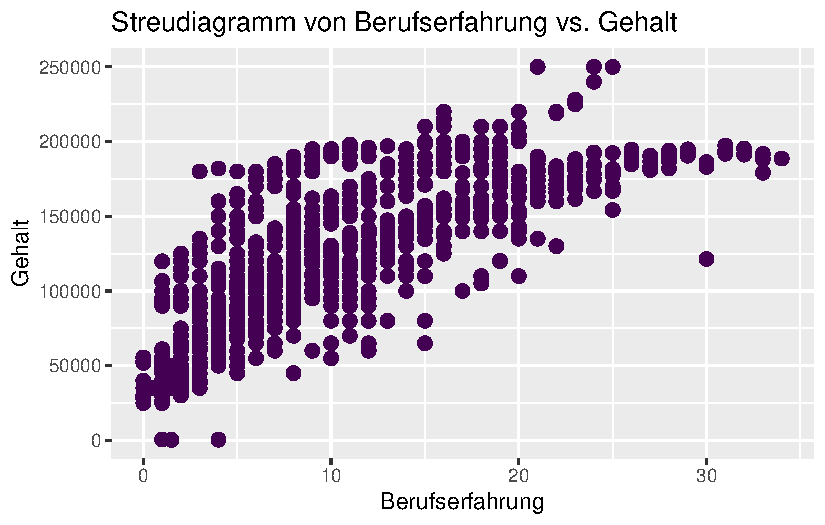
\includegraphics{main_doc_files/figure-pdf/unnamed-chunk-28-1.pdf}

}

\end{figure}

Das Streudiagramm visualisiert deutlich einen eindeutigen aufsteigenden
Trend, der mit einer zunehmenden Anzahl von ``Years of Experience''
einhergeht. Es wird ebenfalls sichtbar, dass die Höchstgehälter von
250.000€ im Bereich von 20 bis 30 Jahren Berufserfahrung konzentriert
sind.

\begin{Shaded}
\begin{Highlighting}[]
\FunctionTok{ggplot}\NormalTok{(salary\_final, }\FunctionTok{aes}\NormalTok{(}\AttributeTok{x =}\NormalTok{ Education.Level, }\AttributeTok{y =}\NormalTok{ Salary)) }\SpecialCharTok{+}
  \FunctionTok{geom\_point}\NormalTok{(}\AttributeTok{color =} \FunctionTok{viridis}\NormalTok{(}\DecValTok{2}\NormalTok{)[}\DecValTok{1}\NormalTok{], }\AttributeTok{size =} \DecValTok{3}\NormalTok{, }\AttributeTok{shape =} \DecValTok{16}\NormalTok{) }\SpecialCharTok{+}
  \FunctionTok{labs}\NormalTok{(}\AttributeTok{title =} \StringTok{"Scatter Plot of Education Level vs Salary"}\NormalTok{,}
       \AttributeTok{x =} \StringTok{"Years of Experience"}\NormalTok{,}
       \AttributeTok{y =} \StringTok{"Salary"}\NormalTok{)}
\end{Highlighting}
\end{Shaded}

\begin{figure}[H]

{\centering 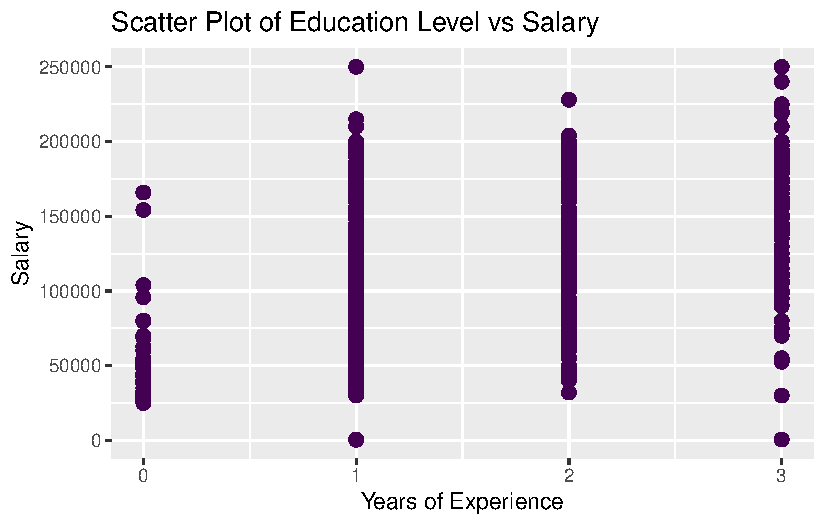
\includegraphics{main_doc_files/figure-pdf/unnamed-chunk-29-1.pdf}

}

\end{figure}

Die vorliegende Datenanalyse verdeutlicht einen klaren Trend zu höheren
Gehaltsklassen, der mit einem Anstieg des Bildungsniveaus einhergeht.
Diese Tendenz wird durch eine erhöhte Dichte in den oberen
Gehaltsgruppen für Personen mit dem dritten Bildungsgrad im Vergleich
zum zweiten und ersten Bildungsgrad deutlich.

\hypertarget{balkendiagramme-mit-2-variablen}{%
\subsection{4.3 Balkendiagramme mit 2
Variablen}\label{balkendiagramme-mit-2-variablen}}

In diesem Abschnitt werden Balkendiagramme verwendet, um den Datensatz
auf Beziehungen zu analysieren. Die visuelle Darstellung durch
Balkendiagramme ermöglicht uns eine anschauliche Interpretation der
Daten.

\hypertarget{average-salary-by-race}{%
\subsubsection{4.3.1 Average Salary by
Race}\label{average-salary-by-race}}

\begin{Shaded}
\begin{Highlighting}[]
\FunctionTok{ggplot}\NormalTok{(salary\_final, }\FunctionTok{aes}\NormalTok{(}\AttributeTok{x =}\NormalTok{ Race, }\AttributeTok{y =}\NormalTok{ Salary, }\AttributeTok{fill =}\NormalTok{ Race)) }\SpecialCharTok{+}
  \FunctionTok{stat\_summary}\NormalTok{(}\AttributeTok{fun =} \StringTok{"mean"}\NormalTok{, }\AttributeTok{geom =} \StringTok{"bar"}\NormalTok{) }\SpecialCharTok{+}
  \FunctionTok{scale\_fill\_viridis}\NormalTok{(}\AttributeTok{discrete =} \ConstantTok{TRUE}\NormalTok{) }\SpecialCharTok{+}
  \FunctionTok{ggtitle}\NormalTok{(}\StringTok{"Durchschnittliches Gehalt nach Ethnizität"}\NormalTok{) }\SpecialCharTok{+}
  \FunctionTok{xlab}\NormalTok{(}\StringTok{"Rasse"}\NormalTok{) }\SpecialCharTok{+}
  \FunctionTok{ylab}\NormalTok{(}\StringTok{"Durchschnittliches Gehalt"}\NormalTok{)}
\end{Highlighting}
\end{Shaded}

\begin{figure}[H]

{\centering 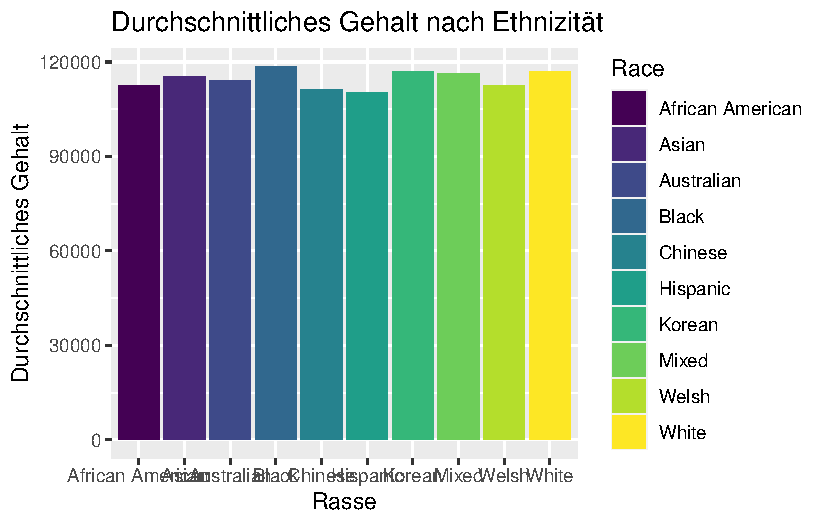
\includegraphics{main_doc_files/figure-pdf/unnamed-chunk-30-1.pdf}

}

\end{figure}

Die Grafik macht deutlich, dass die Gruppen ``Black, Korean, Mixed und
White'' im Durchschnitt am das höchste Einkommen erzielen.

\hypertarget{average-salary-by-country}{%
\subsubsection{4.3.2 Average Salary by
Country}\label{average-salary-by-country}}

\begin{Shaded}
\begin{Highlighting}[]
\FunctionTok{ggplot}\NormalTok{(salary\_final, }\FunctionTok{aes}\NormalTok{(}\AttributeTok{x =}\NormalTok{ Country, }\AttributeTok{y =}\NormalTok{ Salary, }\AttributeTok{fill =}\NormalTok{ Country)) }\SpecialCharTok{+}
  \FunctionTok{stat\_summary}\NormalTok{(}\AttributeTok{fun =} \StringTok{"mean"}\NormalTok{, }\AttributeTok{geom =} \StringTok{"bar"}\NormalTok{, }\AttributeTok{position =} \StringTok{"dodge"}\NormalTok{, }\AttributeTok{color =} \StringTok{"black"}\NormalTok{) }\SpecialCharTok{+}
  \FunctionTok{scale\_fill\_viridis}\NormalTok{(}\AttributeTok{discrete =} \ConstantTok{TRUE}\NormalTok{) }\SpecialCharTok{+}
  \FunctionTok{labs}\NormalTok{(}\AttributeTok{title =} \StringTok{"Durchschnittliches Gehalt nach Land"}\NormalTok{,}
       \AttributeTok{x =} \StringTok{"Land"}\NormalTok{,}
       \AttributeTok{y =} \StringTok{"Durchschnittliches Gehalt"}\NormalTok{) }\SpecialCharTok{+}
  \FunctionTok{theme}\NormalTok{(}\AttributeTok{axis.text.x =} \FunctionTok{element\_text}\NormalTok{(}\AttributeTok{angle =} \DecValTok{45}\NormalTok{, }\AttributeTok{hjust =} \DecValTok{1}\NormalTok{))}
\end{Highlighting}
\end{Shaded}

\begin{figure}[H]

{\centering 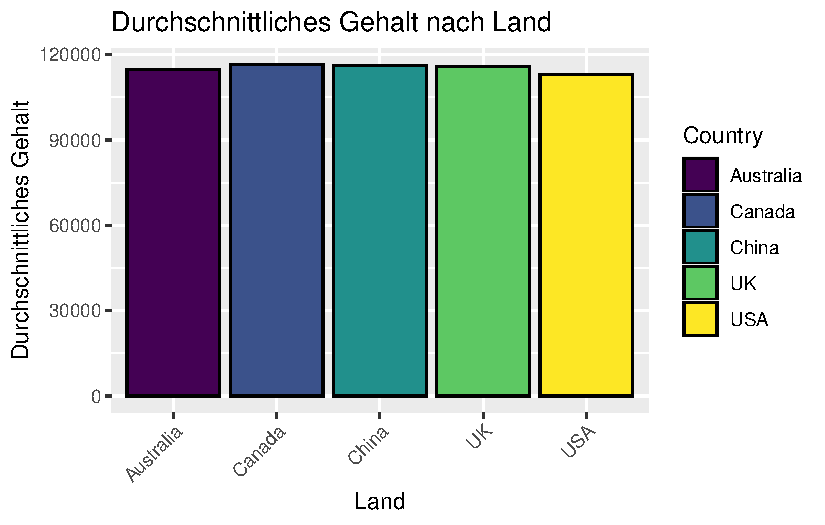
\includegraphics{main_doc_files/figure-pdf/unnamed-chunk-31-1.pdf}

}

\end{figure}

Es ist ersichtlich, dass in den Ländern ``Canada und China'' das
durchschnittliche Gehalt am größten ist. Jedochg ist zu erwähnen, dass
alle Länder nah bei einander liegen.

Es ist ersichtlich, dass in den Ländern ``Canada und China'' das
durchschnittliche Gehalt am höchsten ist. Es ist jedoch zu betonen, dass
die durchschnittlichen Gehälter in allen Ländern nahe beieinander
liegen.

\hypertarget{average-salary-by-country-and-gender}{%
\subsubsection{4.3.3 Average Salary by Country and
Gender}\label{average-salary-by-country-and-gender}}

Die Erstellung eines gestapelten Balkendiagramms ermöglicht uns einen
detaillierten Vergleich der durchschnittlichen Gehälter zwischen
verschiedenen Ländern und Geschlechtern. Die Balken sind entsprechend
nach Geschlecht gruppiert und gestapelt, was eine übersichtliche
Darstellung der Unterschiede in den Gehaltsstrukturen zwischen den
betrachteten Gruppen ermöglicht.

\begin{Shaded}
\begin{Highlighting}[]
\FunctionTok{ggplot}\NormalTok{(salary\_final, }\FunctionTok{aes}\NormalTok{(}\AttributeTok{x =}\NormalTok{ Country, }\AttributeTok{y =}\NormalTok{ Salary, }\AttributeTok{fill =}\NormalTok{ Gender)) }\SpecialCharTok{+}
  \FunctionTok{geom\_bar}\NormalTok{(}\AttributeTok{stat =} \StringTok{"summary"}\NormalTok{, }\AttributeTok{fun =} \StringTok{"mean"}\NormalTok{, }\AttributeTok{position =} \StringTok{"stack"}\NormalTok{, }\AttributeTok{color =} \StringTok{"black"}\NormalTok{) }\SpecialCharTok{+}
  \FunctionTok{scale\_fill\_viridis}\NormalTok{(}\AttributeTok{discrete =} \ConstantTok{TRUE}\NormalTok{) }\SpecialCharTok{+}
  \FunctionTok{labs}\NormalTok{(}\AttributeTok{title =} \StringTok{"Average Salary by Country and Gender"}\NormalTok{,}
       \AttributeTok{x =} \StringTok{"Country"}\NormalTok{,}
       \AttributeTok{y =} \StringTok{"Average Salary"}\NormalTok{) }\SpecialCharTok{+}
  \FunctionTok{theme}\NormalTok{(}\AttributeTok{axis.text.x =} \FunctionTok{element\_text}\NormalTok{(}\AttributeTok{angle =} \DecValTok{45}\NormalTok{, }\AttributeTok{hjust =} \DecValTok{1}\NormalTok{)) }
\end{Highlighting}
\end{Shaded}

\begin{figure}[H]

{\centering 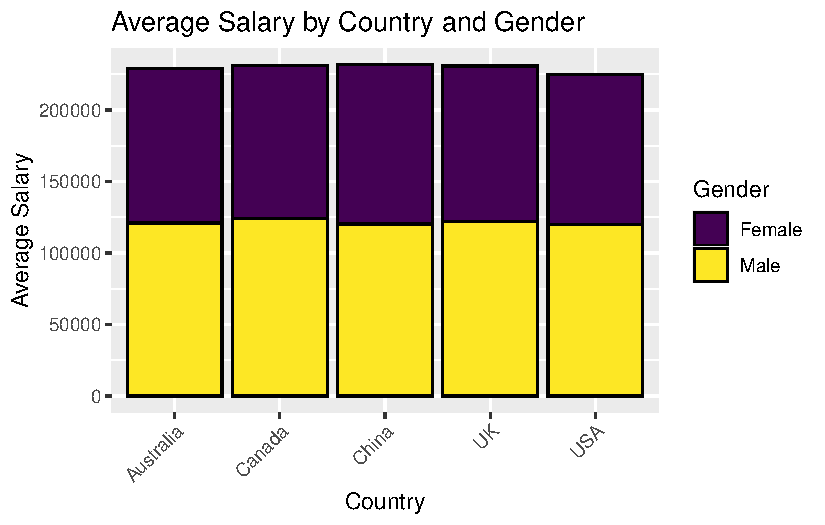
\includegraphics{main_doc_files/figure-pdf/unnamed-chunk-32-1.pdf}

}

\end{figure}

Hier ist zu erkennen, dass alle Länder eine ähnliche Verteilung zwischen
den Geschlechtern ``Male'' und ``Female'' aufweisen.

\hypertarget{average-salary-by-country-and-education-level}{%
\subsubsection{4.3.4 Average Salary by Country and Education
Level}\label{average-salary-by-country-and-education-level}}

Zur Visualisierung der durchnittlichen Bezahlung für Länder und
Bildungsniveau wird ein gruppiertes Balkendiagramm verwendet. Die Balken
sind hierbei nach Bildungsniveau gruppiert.

Zusätzlich wurden die Beschriftungen auf der X-Achse um 45 Grad gedreht,
um eine verbesserte Veranschaulichung zu gewährleisten.

\begin{Shaded}
\begin{Highlighting}[]
\FunctionTok{ggplot}\NormalTok{(salary\_final, }\FunctionTok{aes}\NormalTok{(}\AttributeTok{x =}\NormalTok{ Country, }\AttributeTok{y =}\NormalTok{ Salary, }\AttributeTok{fill =} \FunctionTok{factor}\NormalTok{(Education.Level))) }\SpecialCharTok{+}
  \FunctionTok{geom\_bar}\NormalTok{(}\AttributeTok{stat =} \StringTok{"summary"}\NormalTok{, }\AttributeTok{fun =} \StringTok{"mean"}\NormalTok{, }\AttributeTok{position =} \StringTok{"dodge"}\NormalTok{, }\AttributeTok{color =} \StringTok{"black"}\NormalTok{) }\SpecialCharTok{+}
  \FunctionTok{scale\_fill\_viridis}\NormalTok{(}\AttributeTok{discrete =} \ConstantTok{TRUE}\NormalTok{) }\SpecialCharTok{+}
  \FunctionTok{labs}\NormalTok{(}\AttributeTok{title =} \StringTok{"Average Salary by Country and Education Level"}\NormalTok{,}
       \AttributeTok{x =} \StringTok{"Country"}\NormalTok{,}
       \AttributeTok{y =} \StringTok{"Average Salary"}\NormalTok{) }\SpecialCharTok{+}
  \FunctionTok{theme}\NormalTok{(}\AttributeTok{axis.text.x =} \FunctionTok{element\_text}\NormalTok{(}\AttributeTok{angle =} \DecValTok{45}\NormalTok{, }\AttributeTok{hjust =} \DecValTok{1}\NormalTok{))  }
\end{Highlighting}
\end{Shaded}

\begin{figure}[H]

{\centering 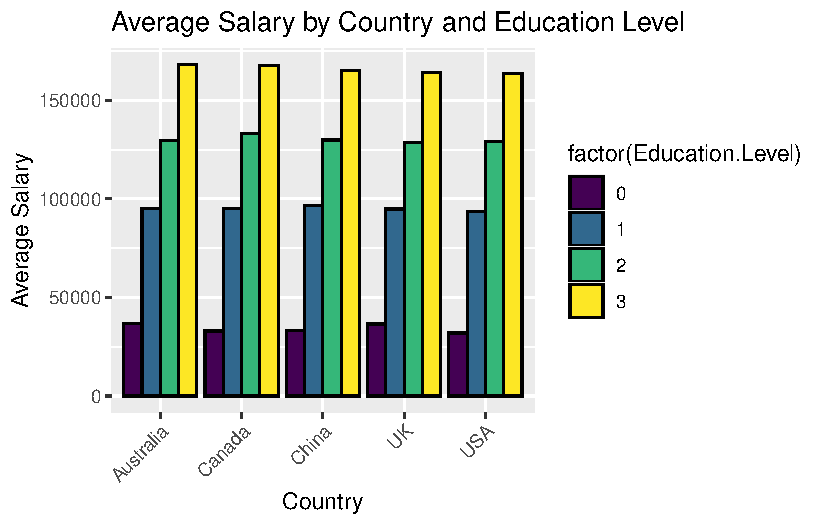
\includegraphics{main_doc_files/figure-pdf/unnamed-chunk-33-1.pdf}

}

\end{figure}

Es ist deutlich zu erkennen, dass die Gehälter in jedem Land deutlich
ansteigen, je höher das Bildungsniveau ist.

\hypertarget{average-salary-by-country-and-race}{%
\subsubsection{4.3.5 Average Salary by Country and
Race}\label{average-salary-by-country-and-race}}

Auch hier wird zum Vergleich der durchschnittlichen Gehälter zwischen
den Ländern und ethnischen Gruppen, ein gestapeltes Balkendiagramm
erstellt. Hierbei sind die Balken nach ethnischer Gruppe gruppiert und
gestapelt.

\begin{Shaded}
\begin{Highlighting}[]
\FunctionTok{ggplot}\NormalTok{(salary\_final, }\FunctionTok{aes}\NormalTok{(}\AttributeTok{x =}\NormalTok{ Country, }\AttributeTok{y =}\NormalTok{ Salary, }\AttributeTok{fill =}\NormalTok{ Race)) }\SpecialCharTok{+}
  \FunctionTok{geom\_bar}\NormalTok{(}\AttributeTok{stat =} \StringTok{"summary"}\NormalTok{, }\AttributeTok{fun =} \StringTok{"mean"}\NormalTok{, }\AttributeTok{position =} \StringTok{"stack"}\NormalTok{, }\AttributeTok{color =} \StringTok{"black"}\NormalTok{) }\SpecialCharTok{+}
  \FunctionTok{scale\_fill\_viridis}\NormalTok{(}\AttributeTok{discrete =} \ConstantTok{TRUE}\NormalTok{) }\SpecialCharTok{+}
  \FunctionTok{labs}\NormalTok{(}\AttributeTok{title =} \StringTok{"Average Salary by Country and Race"}\NormalTok{,}
       \AttributeTok{x =} \StringTok{"Country"}\NormalTok{,}
       \AttributeTok{y =} \StringTok{"Average Salary"}\NormalTok{) }\SpecialCharTok{+}
  \FunctionTok{theme}\NormalTok{(}\AttributeTok{axis.text.x =} \FunctionTok{element\_text}\NormalTok{(}\AttributeTok{angle =} \DecValTok{45}\NormalTok{, }\AttributeTok{hjust =} \DecValTok{1}\NormalTok{)) }\SpecialCharTok{+}
  \FunctionTok{scale\_y\_continuous}\NormalTok{(}\AttributeTok{labels =}\NormalTok{ scales}\SpecialCharTok{::}\NormalTok{comma)}
\end{Highlighting}
\end{Shaded}

\begin{figure}[H]

{\centering 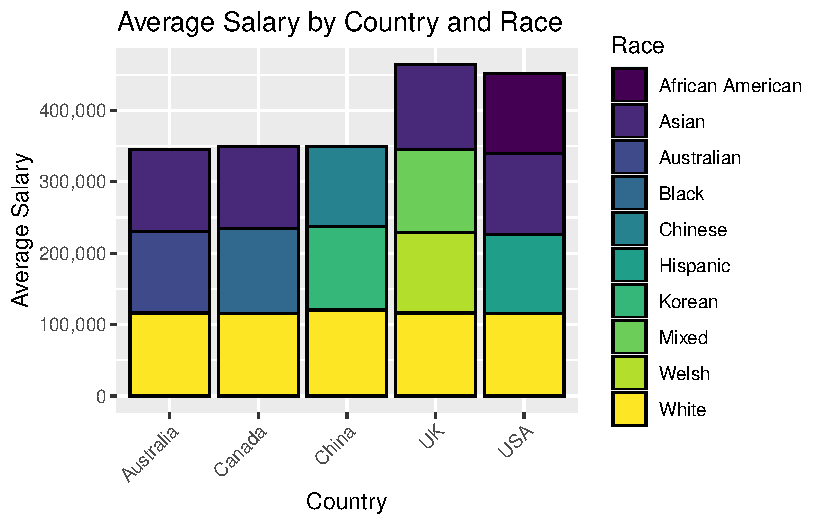
\includegraphics{main_doc_files/figure-pdf/unnamed-chunk-34-1.pdf}

}

\end{figure}

Die Grafik verdeutlicht, dass nicht zwangsläufig in jedem Land alle
ethnischen Gruppen vertreten sind. Es ist ersichtlich, dass nur in 2
Ländern mehr als 3 verschiedene ethnische Gruppen in diesem Datensatz
aufgeführt sind.

\hypertarget{average-salary-by-job-title}{%
\subsubsection{4.3.6 Average Salary by Job
Title}\label{average-salary-by-job-title}}

\begin{Shaded}
\begin{Highlighting}[]
\FunctionTok{ggplot}\NormalTok{(salary\_final, }\FunctionTok{aes}\NormalTok{(}\AttributeTok{x =}\NormalTok{ Job.Title, }\AttributeTok{y =}\NormalTok{ Salary)) }\SpecialCharTok{+}
  \FunctionTok{geom\_bar}\NormalTok{(}\AttributeTok{stat =} \StringTok{"summary"}\NormalTok{, }\AttributeTok{fun =} \StringTok{"mean"}\NormalTok{, }\AttributeTok{color =} \FunctionTok{viridis}\NormalTok{(}\DecValTok{2}\NormalTok{)[}\DecValTok{1}\NormalTok{], }\AttributeTok{color =} \FunctionTok{viridis}\NormalTok{(}\DecValTok{2}\NormalTok{)[}\DecValTok{1}\NormalTok{]) }\SpecialCharTok{+}
  \FunctionTok{scale\_fill\_viridis}\NormalTok{(}\AttributeTok{discrete =} \ConstantTok{TRUE}\NormalTok{) }\SpecialCharTok{+}
  \FunctionTok{labs}\NormalTok{(}\AttributeTok{title =} \StringTok{"Average Salary by Job Title"}\NormalTok{,}
       \AttributeTok{x =} \StringTok{"Job Title"}\NormalTok{,}
       \AttributeTok{y =} \StringTok{"Average Salary"}\NormalTok{) }\SpecialCharTok{+}
  \FunctionTok{theme}\NormalTok{(}\AttributeTok{axis.text.x =} \FunctionTok{element\_text}\NormalTok{(}\AttributeTok{angle =} \DecValTok{45}\NormalTok{, }\AttributeTok{hjust =} \DecValTok{1}\NormalTok{))  }
\end{Highlighting}
\end{Shaded}

\begin{verbatim}
Warning: Duplicated aesthetics after name standardisation: colour
\end{verbatim}

\begin{figure}[H]

{\centering 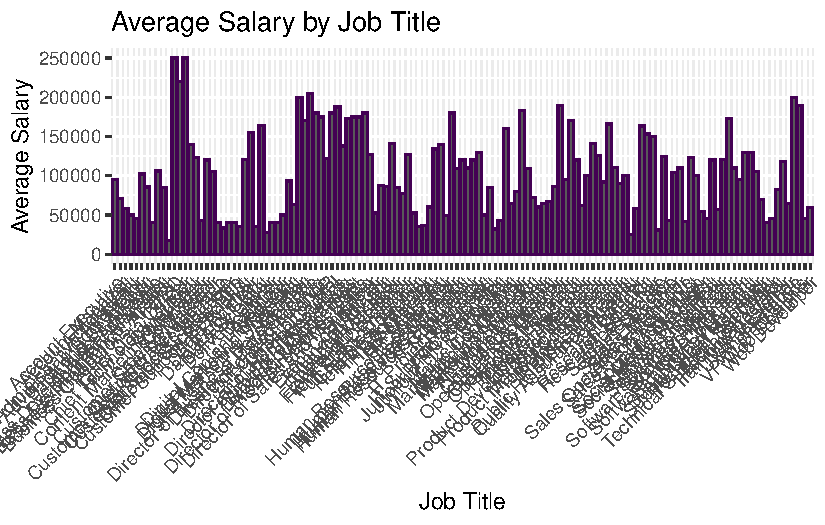
\includegraphics{main_doc_files/figure-pdf/unnamed-chunk-35-1.pdf}

}

\end{figure}

Hier wird festgestellt, dass in dem vorliegenden Datensatz eine hohe
Anzahl von verschiedenen Jobtiteln existiert:

\begin{Shaded}
\begin{Highlighting}[]
\NormalTok{job\_title\_count }\OtherTok{\textless{}{-}} \FunctionTok{table}\NormalTok{(salary\_final}\SpecialCharTok{$}\NormalTok{Job.Title)}
\FunctionTok{print}\NormalTok{(job\_title\_count)}
\end{Highlighting}
\end{Shaded}

\begin{verbatim}

               Account Executive                  Account Manager 
                               1                                4 
                      Accountant         Administrative Assistant 
                               6                                2 
         Advertising Coordinator               Back end Developer 
                               1                              242 
                Business Analyst   Business Development Associate 
                              20                                7 
    Business Development Manager    Business Intelligence Analyst 
                               5                                1 
     Business Operations Analyst                              CEO 
                               2                                1 
              Chief Data Officer         Chief Technology Officer 
                               1                                1 
                      Consultant        Content Marketing Manager 
                               1                               73 
                      Copywriter                Creative Director 
                               2                                1 
        Customer Service Manager             Customer Service Rep 
                               2                                1 
 Customer Service Representative         Customer Success Manager 
                               6                                1 
            Customer Success Rep      Customer Support Specialist 
                               1                                1 
                    Data Analyst                    Data Engineer 
                             391                                4 
                Data Entry Clerk                   Data Scientist 
                               1                              515 
                 Delivery Driver                         Designer 
                               5                                1 
                       Developer         Digital Content Producer 
                               1                                1 
       Digital Marketing Manager     Digital Marketing Specialist 
                              52                               15 
                        Director Director of Business Development 
                               1                                1 
        Director of Data Science          Director of Engineering 
                              57                                2 
             Director of Finance                   Director of HR 
                               2                               69 
       Director of Human Capital      Director of Human Resources 
                               1                                2 
           Director of Marketing           Director of Operations 
                              88                               11 
  Director of Product Management                Director of Sales 
                               1                                1 
 Director of Sales and Marketing                         Engineer 
                               1                                2 
               Event Coordinator                Financial Advisor 
                               2                                5 
               Financial Analyst                Financial Manager 
                              53                              139 
             Front end Developer              Front End Developer 
                             239                               31 
             Full Stack Engineer                 Graphic Designer 
                             304                               23 
               Help Desk Analyst                   HR Coordinator 
                               1                               29 
                   HR Generalist                       HR Manager 
                             104                                5 
                   HR Specialist      Human Resources Coordinator 
                               1                               50 
        Human Resources Director          Human Resources Manager 
                               1                              152 
      Human Resources Specialist                    IT Consultant 
                               1                                2 
                      IT Manager               IT Project Manager 
                               1                                1 
                      IT Support            IT Support Specialist 
                               1                                2 
          Juniour HR Coordinator            Juniour HR Generalist 
                               3                                3 
                         Manager                Marketing Analyst 
                               2                              144 
           Marketing Coordinator               Marketing Director 
                             167                               65 
               Marketing Manager             Marketing Specialist 
                             315                               10 
                Network Engineer                   Office Manager 
                               1                                1 
              Operations Analyst           Operations Coordinator 
                               8                                5 
             Operations Director               Operations Manager 
                               1                              122 
              Principal Engineer              Principal Scientist 
                               1                                1 
                Product Designer      Product Development Manager 
                              80                                1 
                 Product Manager        Product Marketing Manager 
                             323                               70 
             Project Coordinator                 Project Engineer 
                               5                              317 
                 Project Manager         Public Relations Manager 
                              34                                1 
       Quality Assurance Analyst                     Receptionist 
                               1                               57 
                       Recruiter                Research Director 
                               3                               75 
              Research Scientist                       Researcher 
                             119                                1 
                 Sales Associate                   Sales Director 
                             212                               62 
                 Sales Executive                    Sales Manager 
                              38                               58 
        Sales Operations Manager             Sales Representative 
                               1                               81 
                       Scientist                 Social Media Man 
                               3                                1 
            Social Media Manager          Social Media Specialist 
                              15                                2 
              Software Architect               Software Developer 
                               1                              186 
               Software Engineer        Software Engineer Manager 
                             809                              376 
                Software Manager         Software Project Manager 
                               1                                1 
             Strategy Consultant             Supply Chain Analyst 
                               1                                1 
            Supply Chain Manager              Technical Recruiter 
                               1                                1 
    Technical Support Specialist                 Technical Writer 
                               1                                1 
             Training Specialist                      UX Designer 
                               2                                5 
                   UX Researcher                    VP of Finance 
                               1                                1 
                VP of Operations                     Web Designer 
                               1                                1 
                   Web Developer 
                             129 
\end{verbatim}

Hier nochmal umfangreicher grafisch ausgearbeitet:

\begin{Shaded}
\begin{Highlighting}[]
\NormalTok{job\_title\_count }\OtherTok{\textless{}{-}} \FunctionTok{table}\NormalTok{(salary\_final}\SpecialCharTok{$}\NormalTok{Job.Title)}
\NormalTok{job\_title\_df }\OtherTok{\textless{}{-}} \FunctionTok{data.frame}\NormalTok{(}\AttributeTok{Job\_Title =} \FunctionTok{names}\NormalTok{(job\_title\_count), }\AttributeTok{Frequency =} \FunctionTok{as.numeric}\NormalTok{(job\_title\_count))}

\FunctionTok{ggplot}\NormalTok{(job\_title\_df, }\FunctionTok{aes}\NormalTok{(}\AttributeTok{x =}\NormalTok{ Job\_Title, }\AttributeTok{y =}\NormalTok{ Frequency)) }\SpecialCharTok{+}
  \FunctionTok{geom\_bar}\NormalTok{(}\AttributeTok{stat =} \StringTok{"identity"}\NormalTok{, }\AttributeTok{fill =} \FunctionTok{viridis}\NormalTok{(}\DecValTok{2}\NormalTok{)[}\DecValTok{1}\NormalTok{], }\AttributeTok{color =} \StringTok{"black"}\NormalTok{) }\SpecialCharTok{+}
  \FunctionTok{labs}\NormalTok{(}\AttributeTok{title =} \StringTok{"Frequency of Unique Job Titles"}\NormalTok{,}
       \AttributeTok{x =} \StringTok{"Job Titles"}\NormalTok{,}
       \AttributeTok{y =} \StringTok{"Frequency"}\NormalTok{) }\SpecialCharTok{+}
  \FunctionTok{theme}\NormalTok{(}\AttributeTok{axis.text.x =} \FunctionTok{element\_text}\NormalTok{(}\AttributeTok{angle =} \DecValTok{45}\NormalTok{, }\AttributeTok{hjust =} \DecValTok{1}\NormalTok{)) }
\end{Highlighting}
\end{Shaded}

\begin{figure}[H]

{\centering 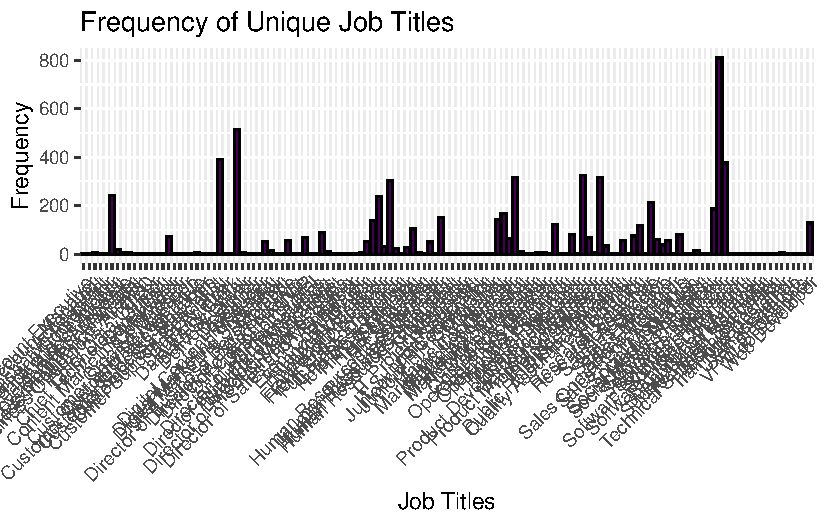
\includegraphics{main_doc_files/figure-pdf/unnamed-chunk-37-1.pdf}

}

\end{figure}

Jeder Job wurde aufgeführt. Es ist anzumerken, dass es aufgrund der
enormen Vielfalt an unterschiedlichen Jobs nicht möglich ist, sämtliche
in der Darstellung zu berücksichtigen.

\begin{Shaded}
\begin{Highlighting}[]
\FunctionTok{library}\NormalTok{(dplyr)}

\NormalTok{job\_title\_count }\OtherTok{\textless{}{-}}\NormalTok{ salary }\SpecialCharTok{\%\textgreater{}\%}
  \FunctionTok{count}\NormalTok{(}\StringTok{\textasciigrave{}}\AttributeTok{Job.Title}\StringTok{\textasciigrave{}}\NormalTok{, }\AttributeTok{sort =} \ConstantTok{TRUE}\NormalTok{)}
\NormalTok{job\_title\_count}
\end{Highlighting}
\end{Shaded}

\begin{verbatim}
# A tibble: 129 x 2
   Job.Title                     n
   <chr>                     <int>
 1 Software Engineer           809
 2 Data Scientist              515
 3 Data Analyst                391
 4 Software Engineer Manager   376
 5 Product Manager             323
 6 Project Engineer            317
 7 Marketing Manager           315
 8 Full Stack Engineer         304
 9 Back end Developer          242
10 Front end Developer         239
# i 119 more rows
\end{verbatim}

\hypertarget{boxplots}{%
\subsection{4.4 Boxplots}\label{boxplots}}

\begin{Shaded}
\begin{Highlighting}[]
\FunctionTok{ggplot}\NormalTok{(salary\_final, }\FunctionTok{aes}\NormalTok{(}\AttributeTok{x =}\NormalTok{ Country, }\AttributeTok{y =}\NormalTok{ Salary, }\AttributeTok{fill =}\NormalTok{ Race)) }\SpecialCharTok{+}
  \FunctionTok{geom\_boxplot}\NormalTok{() }\SpecialCharTok{+}
  \FunctionTok{scale\_fill\_viridis}\NormalTok{(}\AttributeTok{discrete =} \ConstantTok{TRUE}\NormalTok{) }\SpecialCharTok{+}
  \FunctionTok{stat\_summary}\NormalTok{(}\AttributeTok{fun =} \StringTok{"median"}\NormalTok{, }\AttributeTok{geom =} \StringTok{"point"}\NormalTok{, }\AttributeTok{shape =} \DecValTok{18}\NormalTok{, }\AttributeTok{size =} \DecValTok{3}\NormalTok{, }\AttributeTok{color =} \StringTok{"red"}\NormalTok{, }\AttributeTok{position =} \FunctionTok{position\_dodge}\NormalTok{(}\AttributeTok{width =} \FloatTok{0.75}\NormalTok{)) }\SpecialCharTok{+}
  \FunctionTok{labs}\NormalTok{(}\AttributeTok{title =} \StringTok{"Salary Distribution by Country and Race"}\NormalTok{,}
       \AttributeTok{x =} \StringTok{"Country"}\NormalTok{,}
       \AttributeTok{y =} \StringTok{"Salary"}\NormalTok{) }\SpecialCharTok{+}
  \FunctionTok{theme}\NormalTok{(}\AttributeTok{axis.text.x =} \FunctionTok{element\_text}\NormalTok{(}\AttributeTok{angle =} \DecValTok{45}\NormalTok{, }\AttributeTok{hjust =} \DecValTok{1}\NormalTok{))  }
\end{Highlighting}
\end{Shaded}

\begin{figure}[H]

{\centering 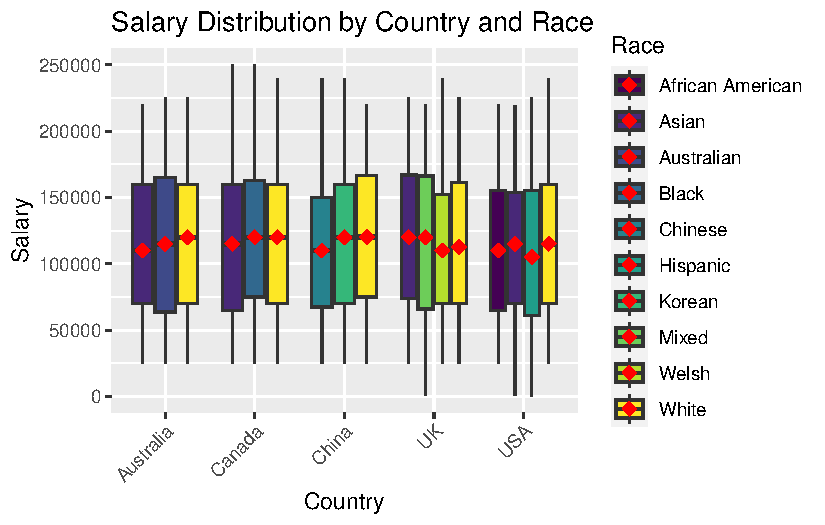
\includegraphics{main_doc_files/figure-pdf/unnamed-chunk-39-1.pdf}

}

\end{figure}

\hypertarget{daten-aufbereiten}{%
\section{5. Daten Aufbereiten}\label{daten-aufbereiten}}

(Tests der Thesen gibt uns die Antwort darauf wie die Daten aufbereitet
werden müssen)

\hypertarget{jobs}{%
\subsection{5.1 Jobs}\label{jobs}}

Da in dem Datensatz teilweise Jobs nur einmalig vertreten sind, kann ein
erhebliches Stichproben-Bias verursacht werden. Da das mittlere
Einkommen ein wichtiges Merkmal in unserer explorativen Datenanalyse
darstellt und mindestens 30 Einträge für eine aussagekräftige Stichprobe
nötig sind, haben wir uns dazu entschlossen alle Einträge mit
N\textless30 bei der Anzahl der Jobtitel (N) abzuschneiden.

\begin{Shaded}
\begin{Highlighting}[]
\NormalTok{filtered\_data }\OtherTok{\textless{}{-}}\NormalTok{ salary\_final }\SpecialCharTok{\%\textgreater{}\%}
  \FunctionTok{group\_by}\NormalTok{(Job.Title) }\SpecialCharTok{\%\textgreater{}\%}
  \FunctionTok{summarise}\NormalTok{(}\AttributeTok{job\_count =} \FunctionTok{n}\NormalTok{()) }\SpecialCharTok{\%\textgreater{}\%}
  \FunctionTok{filter}\NormalTok{(job\_count }\SpecialCharTok{\textgreater{}} \DecValTok{30}\NormalTok{) }\SpecialCharTok{\%\textgreater{}\%}
  \FunctionTok{inner\_join}\NormalTok{(salary\_final, }\AttributeTok{by =} \StringTok{"Job.Title"}\NormalTok{)}

\FunctionTok{print}\NormalTok{(filtered\_data)}
\end{Highlighting}
\end{Shaded}

\begin{verbatim}
# A tibble: 6,398 x 11
   Job.Title   job_count   Age Gender Education.Level Years.Of.Experience Salary
   <chr>           <int> <dbl> <chr>            <dbl>               <dbl>  <dbl>
 1 Back end D~       242    33 Female               2                   5 110000
 2 Back end D~       242    32 Male                 1                   4  95000
 3 Back end D~       242    26 Female               2                   3  90000
 4 Back end D~       242    26 Female               2                   2  70000
 5 Back end D~       242    24 Female               1                   1  60000
 6 Back end D~       242    26 Female               2                   3  90000
 7 Back end D~       242    24 Female               2                   1  60000
 8 Back end D~       242    34 Male                 2                   6 125000
 9 Back end D~       242    29 Female               1                   3  85000
10 Back end D~       242    23 Male                 1                   1  55000
# i 6,388 more rows
# i 4 more variables: Country <chr>, Race <chr>, Senior <dbl>, SalaryKat <fct>
\end{verbatim}

\begin{Shaded}
\begin{Highlighting}[]
\NormalTok{job\_title\_count }\OtherTok{\textless{}{-}} \FunctionTok{table}\NormalTok{(filtered\_data}\SpecialCharTok{$}\NormalTok{Job.Title)}
\FunctionTok{print}\NormalTok{(job\_title\_count)}
\end{Highlighting}
\end{Shaded}

\begin{verbatim}

         Back end Developer   Content Marketing Manager 
                        242                          73 
               Data Analyst              Data Scientist 
                        391                         515 
  Digital Marketing Manager    Director of Data Science 
                         52                          57 
             Director of HR       Director of Marketing 
                         69                          88 
          Financial Analyst           Financial Manager 
                         53                         139 
        Front end Developer         Front End Developer 
                        239                          31 
        Full Stack Engineer               HR Generalist 
                        304                         104 
Human Resources Coordinator     Human Resources Manager 
                         50                         152 
          Marketing Analyst       Marketing Coordinator 
                        144                         167 
         Marketing Director           Marketing Manager 
                         65                         315 
         Operations Manager            Product Designer 
                        122                          80 
            Product Manager   Product Marketing Manager 
                        323                          70 
           Project Engineer             Project Manager 
                        317                          34 
               Receptionist           Research Director 
                         57                          75 
         Research Scientist             Sales Associate 
                        119                         212 
             Sales Director             Sales Executive 
                         62                          38 
              Sales Manager        Sales Representative 
                         58                          81 
         Software Developer           Software Engineer 
                        186                         809 
  Software Engineer Manager               Web Developer 
                        376                         129 
\end{verbatim}

\begin{Shaded}
\begin{Highlighting}[]
\NormalTok{job\_title\_count }\OtherTok{\textless{}{-}} \FunctionTok{table}\NormalTok{(filtered\_data}\SpecialCharTok{$}\NormalTok{Job.Title)}
\NormalTok{job\_title\_df }\OtherTok{\textless{}{-}} \FunctionTok{data.frame}\NormalTok{(}\AttributeTok{Job\_Title =} \FunctionTok{names}\NormalTok{(job\_title\_count), }\AttributeTok{Frequency =} \FunctionTok{as.numeric}\NormalTok{(job\_title\_count))}

\FunctionTok{ggplot}\NormalTok{(job\_title\_df, }\FunctionTok{aes}\NormalTok{(}\AttributeTok{x =}\NormalTok{ Job\_Title, }\AttributeTok{y =}\NormalTok{ Frequency)) }\SpecialCharTok{+}
  \FunctionTok{geom\_bar}\NormalTok{(}\AttributeTok{stat =} \StringTok{"identity"}\NormalTok{, }\AttributeTok{fill =} \FunctionTok{viridis}\NormalTok{(}\DecValTok{2}\NormalTok{)[}\DecValTok{1}\NormalTok{], }\AttributeTok{color =} \StringTok{"black"}\NormalTok{) }\SpecialCharTok{+}
  \FunctionTok{scale\_fill\_viridis}\NormalTok{(}\AttributeTok{discrete =} \ConstantTok{TRUE}\NormalTok{) }\SpecialCharTok{+}
  \FunctionTok{labs}\NormalTok{(}\AttributeTok{title =} \StringTok{"Frequency of Unique Job Titles"}\NormalTok{,}
       \AttributeTok{x =} \StringTok{"Job Titles"}\NormalTok{,}
       \AttributeTok{y =} \StringTok{"Frequency"}\NormalTok{) }\SpecialCharTok{+}
  \FunctionTok{theme}\NormalTok{(}\AttributeTok{axis.text.x =} \FunctionTok{element\_text}\NormalTok{(}\AttributeTok{angle =} \DecValTok{45}\NormalTok{, }\AttributeTok{hjust =} \DecValTok{1}\NormalTok{))}
\end{Highlighting}
\end{Shaded}

\begin{figure}[H]

{\centering 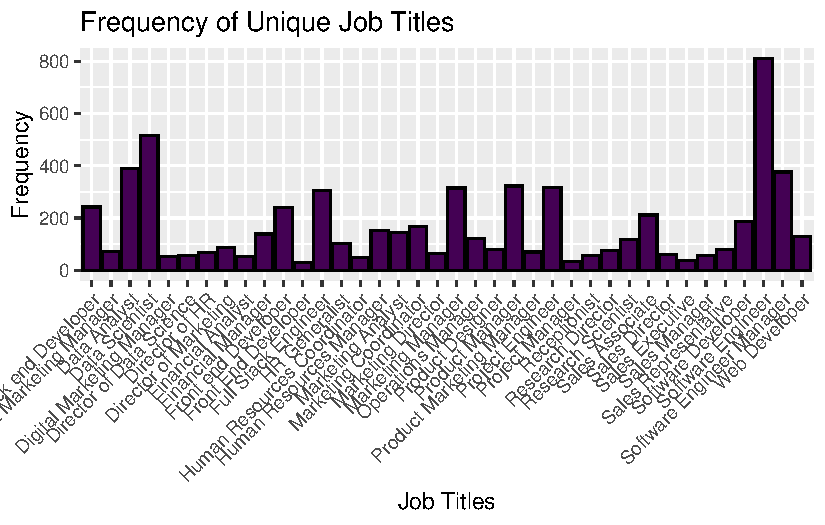
\includegraphics{main_doc_files/figure-pdf/unnamed-chunk-42-1.pdf}

}

\end{figure}

Auf mindestens 30 Jobhäufigkeiten angepasst.

\begin{Shaded}
\begin{Highlighting}[]
\NormalTok{job\_title\_count\_filtered }\OtherTok{\textless{}{-}} \FunctionTok{table}\NormalTok{(filtered\_data}\SpecialCharTok{$}\NormalTok{Job.Title)}
\FunctionTok{cat}\NormalTok{(}\FunctionTok{paste}\NormalTok{(}\FunctionTok{names}\NormalTok{(job\_title\_count\_filtered), }\StringTok{":"}\NormalTok{, job\_title\_count\_filtered, }\StringTok{"}\SpecialCharTok{\textbackslash{}n}\StringTok{"}\NormalTok{))}
\end{Highlighting}
\end{Shaded}

\begin{verbatim}
Back end Developer : 242 
 Content Marketing Manager : 73 
 Data Analyst : 391 
 Data Scientist : 515 
 Digital Marketing Manager : 52 
 Director of Data Science : 57 
 Director of HR : 69 
 Director of Marketing : 88 
 Financial Analyst : 53 
 Financial Manager : 139 
 Front end Developer : 239 
 Front End Developer : 31 
 Full Stack Engineer : 304 
 HR Generalist : 104 
 Human Resources Coordinator : 50 
 Human Resources Manager : 152 
 Marketing Analyst : 144 
 Marketing Coordinator : 167 
 Marketing Director : 65 
 Marketing Manager : 315 
 Operations Manager : 122 
 Product Designer : 80 
 Product Manager : 323 
 Product Marketing Manager : 70 
 Project Engineer : 317 
 Project Manager : 34 
 Receptionist : 57 
 Research Director : 75 
 Research Scientist : 119 
 Sales Associate : 212 
 Sales Director : 62 
 Sales Executive : 38 
 Sales Manager : 58 
 Sales Representative : 81 
 Software Developer : 186 
 Software Engineer : 809 
 Software Engineer Manager : 376 
 Web Developer : 129 
\end{verbatim}

\hypertarget{job-typen}{%
\subsection{5.2 Job Typen}\label{job-typen}}

\hypertarget{anzahl-der-technischen-administrativen-jobs}{%
\subsection{5.2.1 Anzahl der technischen / administrativen
Jobs}\label{anzahl-der-technischen-administrativen-jobs}}

Im Folgenden werden Jobs auf Basis Ihrer Jobtitel in technische und
adminisztrative Kategorien unterteilt. Daraufhin werden die Datensätze
``technische\_jobs'' und ``admin\_Jobs'' erstellt.

\begin{Shaded}
\begin{Highlighting}[]
\CommentTok{\# Filtern nach technischen Jobs}
\NormalTok{technische\_jobs }\OtherTok{\textless{}{-}}\NormalTok{ filtered\_data[}\FunctionTok{grep}\NormalTok{(}\StringTok{"data|engineer|developer|analyst|scientist"}\NormalTok{, }\FunctionTok{tolower}\NormalTok{(filtered\_data}\SpecialCharTok{$}\NormalTok{Job.Title)), ]}

\CommentTok{\# Filtern nach wirtschaftlichen/administrativen Jobs}
\NormalTok{admin\_jobs }\OtherTok{\textless{}{-}}\NormalTok{ filtered\_data[}\FunctionTok{grep}\NormalTok{(}\StringTok{"associate|director|manager|sales|coordinator|generalist|receptionist|designer"}\NormalTok{, }\FunctionTok{tolower}\NormalTok{(filtered\_data}\SpecialCharTok{$}\NormalTok{Job.Title)), ]}

\CommentTok{\# Beispiel für die Ausgabe der ersten paar Zeilen der gefilterten Daten}
\FunctionTok{head}\NormalTok{(technische\_jobs)}
\end{Highlighting}
\end{Shaded}

\begin{verbatim}
# A tibble: 6 x 11
  Job.Title    job_count   Age Gender Education.Level Years.Of.Experience Salary
  <chr>            <int> <dbl> <chr>            <dbl>               <dbl>  <dbl>
1 Back end De~       242    33 Female               2                   5 110000
2 Back end De~       242    32 Male                 1                   4  95000
3 Back end De~       242    26 Female               2                   3  90000
4 Back end De~       242    26 Female               2                   2  70000
5 Back end De~       242    24 Female               1                   1  60000
6 Back end De~       242    26 Female               2                   3  90000
# i 4 more variables: Country <chr>, Race <chr>, Senior <dbl>, SalaryKat <fct>
\end{verbatim}

\begin{Shaded}
\begin{Highlighting}[]
\FunctionTok{head}\NormalTok{(admin\_jobs)}
\end{Highlighting}
\end{Shaded}

\begin{verbatim}
# A tibble: 6 x 11
  Job.Title    job_count   Age Gender Education.Level Years.Of.Experience Salary
  <chr>            <int> <dbl> <chr>            <dbl>               <dbl>  <dbl>
1 Content Mar~        73    30 Female               1                   3  55000
2 Content Mar~        73    27 Female               2                   4  80000
3 Content Mar~        73    27 Female               2                   4  80000
4 Content Mar~        73    27 Female               2                   4  80000
5 Content Mar~        73    27 Female               2                   4  80000
6 Content Mar~        73    27 Female               2                   4  80000
# i 4 more variables: Country <chr>, Race <chr>, Senior <dbl>, SalaryKat <fct>
\end{verbatim}

\begin{Shaded}
\begin{Highlighting}[]
\CommentTok{\# Anzahl der technischen Jobs}
\NormalTok{anzahl\_technische\_jobs }\OtherTok{\textless{}{-}} \FunctionTok{nrow}\NormalTok{(technische\_jobs)}
\FunctionTok{cat}\NormalTok{(}\StringTok{"Anzahl der technischen Jobs:"}\NormalTok{, anzahl\_technische\_jobs, }\StringTok{"}\SpecialCharTok{\textbackslash{}n}\StringTok{"}\NormalTok{)}
\end{Highlighting}
\end{Shaded}

\begin{verbatim}
Anzahl der technischen Jobs: 3912 
\end{verbatim}

\begin{Shaded}
\begin{Highlighting}[]
\CommentTok{\# Anzahl der administrativen Jobs}
\NormalTok{anzahl\_admin\_jobs }\OtherTok{\textless{}{-}} \FunctionTok{nrow}\NormalTok{(admin\_jobs)}
\FunctionTok{cat}\NormalTok{(}\StringTok{"Anzahl der administrativen Jobs:"}\NormalTok{, anzahl\_admin\_jobs, }\StringTok{"}\SpecialCharTok{\textbackslash{}n}\StringTok{"}\NormalTok{)}
\end{Highlighting}
\end{Shaded}

\begin{verbatim}
Anzahl der administrativen Jobs: 2919 
\end{verbatim}

Zu erkennen ist hier, dass es in diesem Datensatz signifikant mehr
technische Jobs als administrative Jobs gibt.

\begin{Shaded}
\begin{Highlighting}[]
\CommentTok{\# Anzahl der Zeilen (Werte) in filtered\_data}
\NormalTok{anzahl\_werte\_filtered\_data }\OtherTok{\textless{}{-}} \FunctionTok{nrow}\NormalTok{(filtered\_data)}

\CommentTok{\# Anzeigen der Anzahl der Werte}
\FunctionTok{cat}\NormalTok{(}\StringTok{"Anzahl der Werte in filtered\_data:"}\NormalTok{, anzahl\_werte\_filtered\_data, }\StringTok{"}\SpecialCharTok{\textbackslash{}n}\StringTok{"}\NormalTok{)}
\end{Highlighting}
\end{Shaded}

\begin{verbatim}
Anzahl der Werte in filtered_data: 6398 
\end{verbatim}

Insgesamt gibt es in dem gefilterten Datensatz 6398 Einträge, was
bedeutet, dass es sich bei ungefähr 60\% um technische Jobs handelt und
40\% administrative Jobs sind.

Nun wird nochmal der gefilterte Datensatz mit der Summe von
``anzahl\_technische\_jobs'' und ``anzahl\_administraive Jobs''
verglichen.

\begin{Shaded}
\begin{Highlighting}[]
\NormalTok{anzahl\_jobs }\OtherTok{\textless{}{-}}\NormalTok{ anzahl\_technische\_jobs }\SpecialCharTok{+}\NormalTok{ anzahl\_admin\_jobs}
\FunctionTok{cat}\NormalTok{(anzahl\_jobs)}
\end{Highlighting}
\end{Shaded}

\begin{verbatim}
6831
\end{verbatim}

Zu erkennen ist hier, dass es zwei unterschiedliche Werte für die beiden
Datensätze gibt.

Wir vermuten, dass einige Jobs doppelt gezählt werden. Dies würde
erklären, dass deutlich mehr Einträge in ``anzahl\_jobs'' sind. Unser
Lösungsvorschlag wäre hier, dass wir den Jobs IDs geben.

\hypertarget{luxf6sungsansatz-1}{%
\paragraph{5.2.1.1 Lösungsansatz 1}\label{luxf6sungsansatz-1}}

Der erste Lösungsansatz sieht wie folgt aus:

Die Jobs werden durch Filter anhand bestimmter Namen (wie ``data'',
``engineer'' usw.) ausgewählt und alle Duplikate entfernt. Das Ergebnis
ist nun ein neuer Datensatz namens ``filtered\_data\_neu'', der alle
Zeilen außer die mit technischen und administrativen Jobs enthält.

\begin{Shaded}
\begin{Highlighting}[]
\NormalTok{filtered\_data}\SpecialCharTok{$}\NormalTok{ID }\OtherTok{\textless{}{-}} \DecValTok{1}\SpecialCharTok{:}\FunctionTok{nrow}\NormalTok{(filtered\_data)}

\NormalTok{technische\_jobs2 }\OtherTok{\textless{}{-}} \FunctionTok{unique}\NormalTok{(filtered\_data[}\FunctionTok{grep}\NormalTok{(}\StringTok{"data|engineer|developer|analyst|scientist"}\NormalTok{, }\FunctionTok{tolower}\NormalTok{(filtered\_data}\SpecialCharTok{$}\NormalTok{Job.Title)), ])}

\NormalTok{admin\_jobs2 }\OtherTok{\textless{}{-}} \FunctionTok{unique}\NormalTok{(filtered\_data[}\FunctionTok{grep}\NormalTok{(}\StringTok{"associate|director|manager|sales|coordinator|generalist|receptionist|designer"}\NormalTok{, }\FunctionTok{tolower}\NormalTok{(filtered\_data}\SpecialCharTok{$}\NormalTok{Job.Title)), ])}

\NormalTok{ids\_technische\_jobs }\OtherTok{\textless{}{-}}\NormalTok{ filtered\_data}\SpecialCharTok{$}\NormalTok{ID[filtered\_data}\SpecialCharTok{$}\NormalTok{Job.Title }\SpecialCharTok{\%in\%}\NormalTok{ technische\_jobs2}\SpecialCharTok{$}\NormalTok{Job.Title]}
\NormalTok{ids\_admin\_jobs }\OtherTok{\textless{}{-}}\NormalTok{ filtered\_data}\SpecialCharTok{$}\NormalTok{ID[filtered\_data}\SpecialCharTok{$}\NormalTok{Job.Title }\SpecialCharTok{\%in\%}\NormalTok{ admin\_jobs2}\SpecialCharTok{$}\NormalTok{Job.Title]}

\CommentTok{\# Entferne die entsprechenden Zeilen aus filtered\_data}
\NormalTok{filtered\_data\_neu }\OtherTok{\textless{}{-}}\NormalTok{ filtered\_data[}\SpecialCharTok{!}\NormalTok{(filtered\_data}\SpecialCharTok{$}\NormalTok{ID }\SpecialCharTok{\%in\%} \FunctionTok{c}\NormalTok{(ids\_technische\_jobs, ids\_admin\_jobs)), ]}

\CommentTok{\# Beispiel für die Ausgabe der ersten paar Zeilen der gefilterten Daten}
\FunctionTok{head}\NormalTok{(filtered\_data\_neu)}
\end{Highlighting}
\end{Shaded}

\begin{verbatim}
# A tibble: 0 x 12
# i 12 variables: Job.Title <chr>, job_count <int>, Age <dbl>, Gender <chr>,
#   Education.Level <dbl>, Years.Of.Experience <dbl>, Salary <dbl>,
#   Country <chr>, Race <chr>, Senior <dbl>, SalaryKat <fct>, ID <int>
\end{verbatim}

\begin{Shaded}
\begin{Highlighting}[]
\NormalTok{anzahl\_technische\_jobs2 }\OtherTok{\textless{}{-}} \FunctionTok{nrow}\NormalTok{(technische\_jobs2)}
\FunctionTok{cat}\NormalTok{(}\StringTok{"Anzahl der technischen Jobs2:"}\NormalTok{, anzahl\_technische\_jobs2, }\StringTok{"}\SpecialCharTok{\textbackslash{}n}\StringTok{"}\NormalTok{)}
\end{Highlighting}
\end{Shaded}

\begin{verbatim}
Anzahl der technischen Jobs2: 3912 
\end{verbatim}

\begin{Shaded}
\begin{Highlighting}[]
\NormalTok{anzahl\_admin\_jobs2 }\OtherTok{\textless{}{-}} \FunctionTok{nrow}\NormalTok{(admin\_jobs2)}
\FunctionTok{cat}\NormalTok{(}\StringTok{"Anzahl der administrativen Jobs2:"}\NormalTok{, anzahl\_admin\_jobs2, }\StringTok{"}\SpecialCharTok{\textbackslash{}n}\StringTok{"}\NormalTok{)}
\end{Highlighting}
\end{Shaded}

\begin{verbatim}
Anzahl der administrativen Jobs2: 2919 
\end{verbatim}

Es scheint als würde dieser Lösungsansatz nicht funktionieren, da der
neue Datensatz keine Einträge enthält.

\hypertarget{luxf6sungsansatz-2}{%
\paragraph{5.2.1.2 Lösungsansatz 2}\label{luxf6sungsansatz-2}}

Der zweite Lösungsansatz für das Problem der Klassifizierung der
verschiedenen Jobtypen besteht darin, dass nicht in zwei Tabellen
unterteilt wird, sondern dass jeder Zeile ein Wert des entsprechenden
Jobtyps zugeordnet wird.

\begin{Shaded}
\begin{Highlighting}[]
\NormalTok{filtered\_data}\SpecialCharTok{$}\NormalTok{job\_type }\OtherTok{\textless{}{-}} \FunctionTok{ifelse}\NormalTok{(}
    \FunctionTok{grepl}\NormalTok{(}\StringTok{"data|engineer|developer|analyst|scientist"}\NormalTok{, }\FunctionTok{tolower}\NormalTok{(filtered\_data}\SpecialCharTok{$}\NormalTok{Job.Title)),}
    \DecValTok{0}\NormalTok{, }\CommentTok{\# 0 für technische Jobs}
    \FunctionTok{ifelse}\NormalTok{(}
        \FunctionTok{grepl}\NormalTok{(}\StringTok{"associate|director|manager|sales|coordinator|generalist"}\NormalTok{, }\FunctionTok{tolower}\NormalTok{(filtered\_data}\SpecialCharTok{$}\NormalTok{Job.Title)),}
        \DecValTok{1}\NormalTok{, }\CommentTok{\# 1 für administrative Jobs}
        \ConstantTok{NA}  \CommentTok{\# NA für alle anderen}
\NormalTok{    )}
\NormalTok{)}

\NormalTok{total\_rows }\OtherTok{\textless{}{-}} \FunctionTok{nrow}\NormalTok{(filtered\_data)}
\NormalTok{count\_job\_types }\OtherTok{\textless{}{-}} \FunctionTok{table}\NormalTok{(filtered\_data}\SpecialCharTok{$}\NormalTok{job\_type, }\AttributeTok{useNA =} \StringTok{"ifany"}\NormalTok{)}

\FunctionTok{print}\NormalTok{(}\FunctionTok{paste}\NormalTok{(}\StringTok{"Gesamtanzahl der Zeilen im Datensatz:"}\NormalTok{, total\_rows))}
\end{Highlighting}
\end{Shaded}

\begin{verbatim}
[1] "Gesamtanzahl der Zeilen im Datensatz: 6398"
\end{verbatim}

\begin{Shaded}
\begin{Highlighting}[]
\FunctionTok{print}\NormalTok{(}\StringTok{"Anzahl der Zeilen für jede job\_type{-}Ausprägung:"}\NormalTok{)}
\end{Highlighting}
\end{Shaded}

\begin{verbatim}
[1] "Anzahl der Zeilen für jede job_type-Ausprägung:"
\end{verbatim}

\begin{Shaded}
\begin{Highlighting}[]
\FunctionTok{print}\NormalTok{(count\_job\_types)}
\end{Highlighting}
\end{Shaded}

\begin{verbatim}

   0    1 <NA> 
3912 2349  137 
\end{verbatim}

Es wird eine neue Spalte namens ``job\_type'' erstellt und mit Werten
gefüllt. Dabei wird der Wert 0 für Zeilen mit technischen Jobs, 1 für
administrative Jobs und NA für alle anderen Jobtypen vergeben.

Nun werden die eben gefundenen NAs in einen neuen Datensatz geschrieben.

\begin{Shaded}
\begin{Highlighting}[]
\NormalTok{na\_job\_type\_rows }\OtherTok{\textless{}{-}} \FunctionTok{subset}\NormalTok{(filtered\_data, }\FunctionTok{is.na}\NormalTok{(job\_type))}

\NormalTok{na\_job\_type\_rows}
\end{Highlighting}
\end{Shaded}

\begin{verbatim}
# A tibble: 137 x 13
   Job.Title   job_count   Age Gender Education.Level Years.Of.Experience Salary
   <chr>           <int> <dbl> <chr>            <dbl>               <dbl>  <dbl>
 1 Product De~        80    33 Male                 2                   6  90000
 2 Product De~        80    43 Female               3                  18 140000
 3 Product De~        80    45 Female               3                  15 150000
 4 Product De~        80    45 Female               3                  15 150000
 5 Product De~        80    44 Female               3                  15 150000
 6 Product De~        80    44 Female               3                  15 150000
 7 Product De~        80    27 Male                 1                   3  60000
 8 Product De~        80    27 Male                 1                   3  60000
 9 Product De~        80    27 Male                 1                   3  60000
10 Product De~        80    27 Male                 1                   3  60000
# i 127 more rows
# i 6 more variables: Country <chr>, Race <chr>, Senior <dbl>, SalaryKat <fct>,
#   ID <int>, job_type <dbl>
\end{verbatim}

Das Ergebnis dieser Abfrage ist eine Tabelle, welche nur aus Product
Designer \% Receptionist besteht. Diese werden nun den adminsitrativen
Jobs hinzugefügt.

\begin{Shaded}
\begin{Highlighting}[]
\NormalTok{filtered\_data}\SpecialCharTok{$}\NormalTok{job\_type[filtered\_data}\SpecialCharTok{$}\NormalTok{Job.Title }\SpecialCharTok{\%in\%} \FunctionTok{c}\NormalTok{(}\StringTok{"Product Designer"}\NormalTok{, }\StringTok{"Receptionist"}\NormalTok{)] }\OtherTok{\textless{}{-}} \DecValTok{1}

\FunctionTok{subset}\NormalTok{(filtered\_data, Job.Title }\SpecialCharTok{\%in\%} \FunctionTok{c}\NormalTok{(}\StringTok{"Product Designer"}\NormalTok{, }\StringTok{"Receptionist"}\NormalTok{))}
\end{Highlighting}
\end{Shaded}

\begin{verbatim}
# A tibble: 137 x 13
   Job.Title   job_count   Age Gender Education.Level Years.Of.Experience Salary
   <chr>           <int> <dbl> <chr>            <dbl>               <dbl>  <dbl>
 1 Product De~        80    33 Male                 2                   6  90000
 2 Product De~        80    43 Female               3                  18 140000
 3 Product De~        80    45 Female               3                  15 150000
 4 Product De~        80    45 Female               3                  15 150000
 5 Product De~        80    44 Female               3                  15 150000
 6 Product De~        80    44 Female               3                  15 150000
 7 Product De~        80    27 Male                 1                   3  60000
 8 Product De~        80    27 Male                 1                   3  60000
 9 Product De~        80    27 Male                 1                   3  60000
10 Product De~        80    27 Male                 1                   3  60000
# i 127 more rows
# i 6 more variables: Country <chr>, Race <chr>, Senior <dbl>, SalaryKat <fct>,
#   ID <int>, job_type <dbl>
\end{verbatim}

\begin{Shaded}
\begin{Highlighting}[]
\NormalTok{total\_rows }\OtherTok{\textless{}{-}} \FunctionTok{nrow}\NormalTok{(filtered\_data)}
\NormalTok{count\_job\_types }\OtherTok{\textless{}{-}} \FunctionTok{table}\NormalTok{(filtered\_data}\SpecialCharTok{$}\NormalTok{job\_type, }\AttributeTok{useNA =} \StringTok{"ifany"}\NormalTok{)}

\FunctionTok{print}\NormalTok{(}\FunctionTok{paste}\NormalTok{(}\StringTok{"Gesamtanzahl der Zeilen im Datensatz:"}\NormalTok{, total\_rows))}
\end{Highlighting}
\end{Shaded}

\begin{verbatim}
[1] "Gesamtanzahl der Zeilen im Datensatz: 6398"
\end{verbatim}

\begin{Shaded}
\begin{Highlighting}[]
\FunctionTok{print}\NormalTok{(}\StringTok{"Anzahl der Zeilen für jede job\_type{-}Ausprägung:"}\NormalTok{)}
\end{Highlighting}
\end{Shaded}

\begin{verbatim}
[1] "Anzahl der Zeilen für jede job_type-Ausprägung:"
\end{verbatim}

\begin{Shaded}
\begin{Highlighting}[]
\FunctionTok{print}\NormalTok{(count\_job\_types)}
\end{Highlighting}
\end{Shaded}

\begin{verbatim}

   0    1 
3912 2486 
\end{verbatim}

Nun ist das Klassifizierungsproblem gelöst. Aufgrund dessen können jetzt
auch Diagramme über Job\_types ausgewertet werden.

\hypertarget{zugewanderte-expats-einheimische}{%
\subsection{5.3 Zugewanderte ( Expats ) \&
Einheimische}\label{zugewanderte-expats-einheimische}}

Im Folgenden werden einige Boxplots erstellt.

\hypertarget{years-of-experience-vs.-gender}{%
\subsubsection{5.3.1 Years of Experience
vs.~Gender}\label{years-of-experience-vs.-gender}}

\begin{Shaded}
\begin{Highlighting}[]
\FunctionTok{ggplot}\NormalTok{(filtered\_data, }\FunctionTok{aes}\NormalTok{(}\AttributeTok{x =} \FunctionTok{factor}\NormalTok{(Gender), }\AttributeTok{y =}\NormalTok{ Years.Of.Experience, }\AttributeTok{fill =}\NormalTok{ Gender)) }\SpecialCharTok{+}
  \FunctionTok{geom\_boxplot}\NormalTok{(}\AttributeTok{alpha =} \FloatTok{0.7}\NormalTok{) }\SpecialCharTok{+}
  \FunctionTok{scale\_fill\_viridis}\NormalTok{(}\AttributeTok{discrete =} \ConstantTok{TRUE}\NormalTok{) }\SpecialCharTok{+}
  \FunctionTok{labs}\NormalTok{(}\AttributeTok{title =} \StringTok{"Boxplot: Years of Experience vs. Gender"}\NormalTok{,}
       \AttributeTok{x =} \StringTok{"Gender"}\NormalTok{,}
       \AttributeTok{y =} \StringTok{"Years of Experience"}\NormalTok{,}
       \AttributeTok{fill =} \StringTok{"Gender"}\NormalTok{) }\SpecialCharTok{+}
  \FunctionTok{theme\_minimal}\NormalTok{()}
\end{Highlighting}
\end{Shaded}

\begin{figure}[H]

{\centering 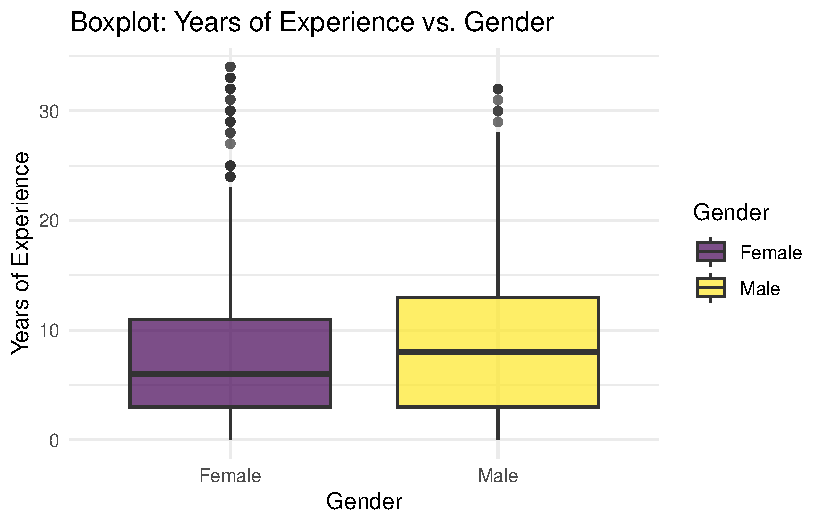
\includegraphics{main_doc_files/figure-pdf/unnamed-chunk-53-1.pdf}

}

\end{figure}

\hypertarget{years-of-experience-vs.-gender-china}{%
\subsubsection{5.3.2 Years of Experience vs.~Gender
(China)}\label{years-of-experience-vs.-gender-china}}

\begin{Shaded}
\begin{Highlighting}[]
\FunctionTok{library}\NormalTok{(ggplot2)}

\NormalTok{data\_china }\OtherTok{\textless{}{-}} \FunctionTok{subset}\NormalTok{(filtered\_data, Country }\SpecialCharTok{==} \StringTok{"China"}\NormalTok{)}

\FunctionTok{ggplot}\NormalTok{(data\_china, }\FunctionTok{aes}\NormalTok{(}\AttributeTok{x =} \FunctionTok{factor}\NormalTok{(Gender), }\AttributeTok{y =}\NormalTok{ Years.Of.Experience, }\AttributeTok{fill =}\NormalTok{ Gender)) }\SpecialCharTok{+}
  \FunctionTok{geom\_boxplot}\NormalTok{(}\AttributeTok{alpha =} \FloatTok{0.7}\NormalTok{) }\SpecialCharTok{+}
  \FunctionTok{scale\_fill\_viridis}\NormalTok{(}\AttributeTok{discrete =} \ConstantTok{TRUE}\NormalTok{) }\SpecialCharTok{+}
  \FunctionTok{labs}\NormalTok{(}\AttributeTok{title =} \StringTok{"Boxplot: Years of Experience vs. Gender (China)"}\NormalTok{,}
       \AttributeTok{x =} \StringTok{"Gender"}\NormalTok{,}
       \AttributeTok{y =} \StringTok{"Years of Experience"}\NormalTok{,}
       \AttributeTok{fill =} \StringTok{"Gender"}\NormalTok{) }\SpecialCharTok{+}
  \FunctionTok{theme\_minimal}\NormalTok{()}
\end{Highlighting}
\end{Shaded}

\begin{figure}[H]

{\centering 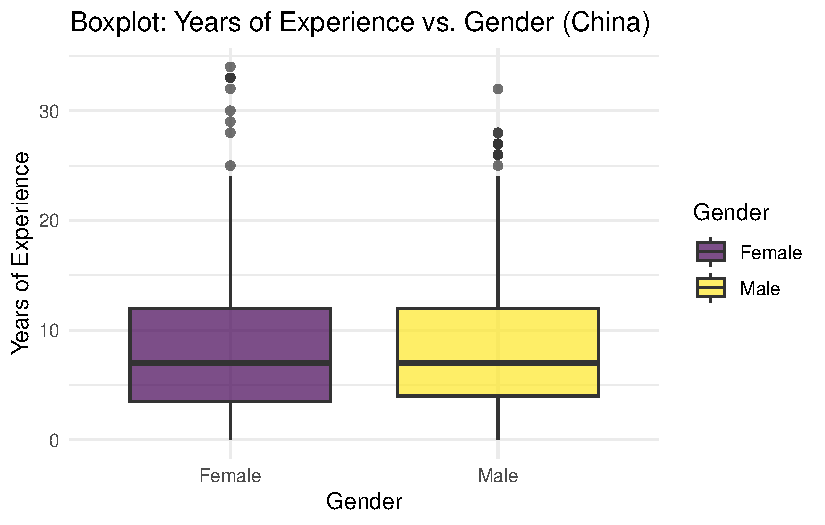
\includegraphics{main_doc_files/figure-pdf/unnamed-chunk-54-1.pdf}

}

\end{figure}

\hypertarget{years-of-experience-vs.-gender-usa}{%
\subsubsection{5.3.3 Years of Experience vs.~Gender(
USA)}\label{years-of-experience-vs.-gender-usa}}

\begin{Shaded}
\begin{Highlighting}[]
\FunctionTok{library}\NormalTok{(ggplot2)}

\NormalTok{data\_usa }\OtherTok{\textless{}{-}} \FunctionTok{subset}\NormalTok{(filtered\_data, Country }\SpecialCharTok{==} \StringTok{"USA"}\NormalTok{)}

\FunctionTok{ggplot}\NormalTok{(data\_usa, }\FunctionTok{aes}\NormalTok{(}\AttributeTok{x =} \FunctionTok{factor}\NormalTok{(Gender), }\AttributeTok{y =}\NormalTok{ Years.Of.Experience, }\AttributeTok{fill =}\NormalTok{ Gender)) }\SpecialCharTok{+}
  \FunctionTok{geom\_boxplot}\NormalTok{(}\AttributeTok{alpha =} \FloatTok{0.7}\NormalTok{) }\SpecialCharTok{+}
  \FunctionTok{scale\_fill\_viridis}\NormalTok{(}\AttributeTok{discrete =} \ConstantTok{TRUE}\NormalTok{) }\SpecialCharTok{+}
  \FunctionTok{labs}\NormalTok{(}\AttributeTok{title =} \StringTok{"Boxplot: Years of Experience vs. Gender (USA)"}\NormalTok{,}
       \AttributeTok{x =} \StringTok{"Gender"}\NormalTok{,}
       \AttributeTok{y =} \StringTok{"Years of Experience"}\NormalTok{,}
       \AttributeTok{fill =} \StringTok{"Gender"}\NormalTok{) }\SpecialCharTok{+}
  \FunctionTok{theme\_minimal}\NormalTok{()}
\end{Highlighting}
\end{Shaded}

\begin{figure}[H]

{\centering 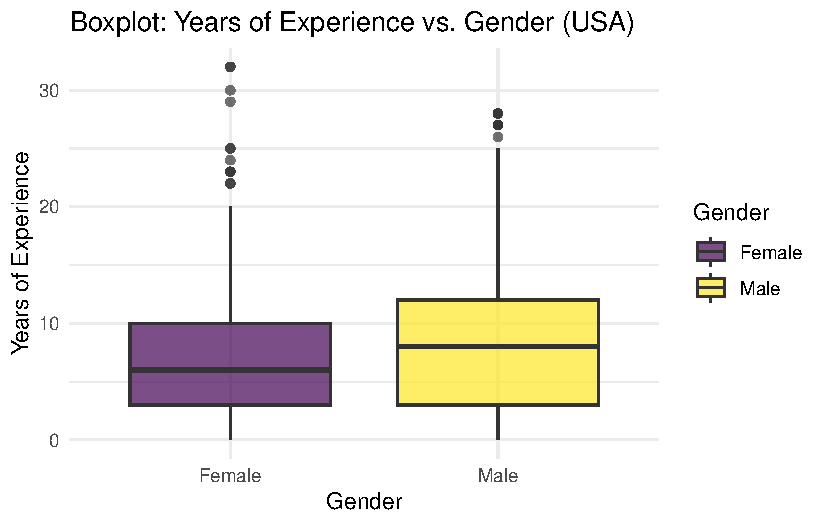
\includegraphics{main_doc_files/figure-pdf/unnamed-chunk-55-1.pdf}

}

\end{figure}

\hypertarget{salary-vs.-gender-china}{%
\subsubsection{5.3.4 Salary vs.~Gender (
China)}\label{salary-vs.-gender-china}}

\begin{Shaded}
\begin{Highlighting}[]
\FunctionTok{library}\NormalTok{(ggplot2)}

\NormalTok{data\_china }\OtherTok{\textless{}{-}} \FunctionTok{subset}\NormalTok{(filtered\_data, Country }\SpecialCharTok{==} \StringTok{"China"}\NormalTok{)}

\FunctionTok{ggplot}\NormalTok{(data\_china, }\FunctionTok{aes}\NormalTok{(}\AttributeTok{x =} \FunctionTok{factor}\NormalTok{(Gender), }\AttributeTok{y =}\NormalTok{ Salary, }\AttributeTok{fill =}\NormalTok{ Gender)) }\SpecialCharTok{+}
  \FunctionTok{geom\_boxplot}\NormalTok{(}\AttributeTok{alpha =} \FloatTok{0.7}\NormalTok{) }\SpecialCharTok{+}
  \FunctionTok{scale\_fill\_viridis}\NormalTok{(}\AttributeTok{discrete =} \ConstantTok{TRUE}\NormalTok{) }\SpecialCharTok{+}
  \FunctionTok{labs}\NormalTok{(}\AttributeTok{title =} \StringTok{"Boxplot: Salary vs. Gender (China)"}\NormalTok{,}
       \AttributeTok{x =} \StringTok{"Gender"}\NormalTok{,}
       \AttributeTok{y =} \StringTok{"Salary"}\NormalTok{,}
       \AttributeTok{fill =} \StringTok{"Gender"}\NormalTok{) }\SpecialCharTok{+}
  \FunctionTok{theme\_minimal}\NormalTok{()}
\end{Highlighting}
\end{Shaded}

\begin{figure}[H]

{\centering 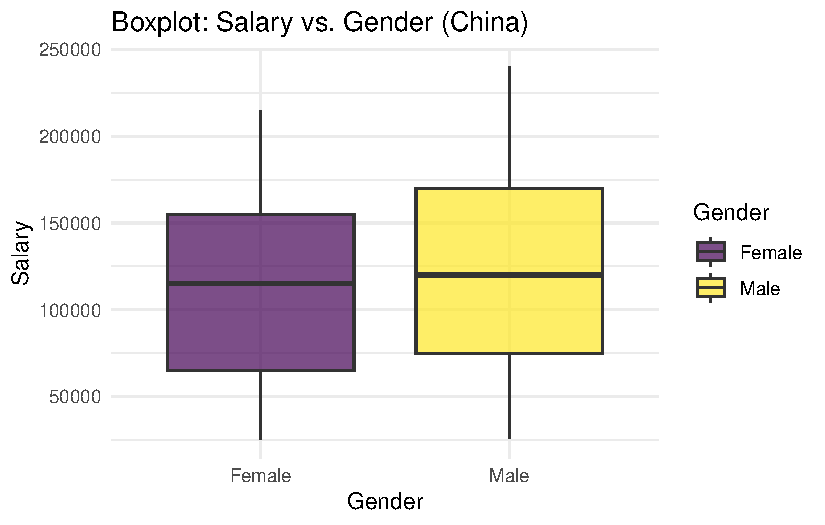
\includegraphics{main_doc_files/figure-pdf/unnamed-chunk-56-1.pdf}

}

\end{figure}

\hypertarget{salary-vs.-gender-usa}{%
\subsubsection{5.3.5 Salary vs.~Gender
(USA)}\label{salary-vs.-gender-usa}}

\begin{Shaded}
\begin{Highlighting}[]
\FunctionTok{library}\NormalTok{(ggplot2)}

\NormalTok{data\_usa }\OtherTok{\textless{}{-}} \FunctionTok{subset}\NormalTok{(filtered\_data, Country }\SpecialCharTok{==} \StringTok{"USA"}\NormalTok{)}

\FunctionTok{ggplot}\NormalTok{(data\_usa, }\FunctionTok{aes}\NormalTok{(}\AttributeTok{x =} \FunctionTok{factor}\NormalTok{(Gender), }\AttributeTok{y =}\NormalTok{ Salary, }\AttributeTok{fill =}\NormalTok{ Gender)) }\SpecialCharTok{+}
  \FunctionTok{geom\_boxplot}\NormalTok{(}\AttributeTok{alpha =} \FloatTok{0.7}\NormalTok{) }\SpecialCharTok{+}
  \FunctionTok{scale\_fill\_viridis}\NormalTok{(}\AttributeTok{discrete =} \ConstantTok{TRUE}\NormalTok{) }\SpecialCharTok{+}
  \FunctionTok{labs}\NormalTok{(}\AttributeTok{title =} \StringTok{"Boxplot: Salary vs. Gender (USA)"}\NormalTok{,}
       \AttributeTok{x =} \StringTok{"Gender"}\NormalTok{,}
       \AttributeTok{y =} \StringTok{"Salary"}\NormalTok{,}
       \AttributeTok{fill =} \StringTok{"Gender"}\NormalTok{) }\SpecialCharTok{+}
  \FunctionTok{theme\_minimal}\NormalTok{()}
\end{Highlighting}
\end{Shaded}

\begin{figure}[H]

{\centering 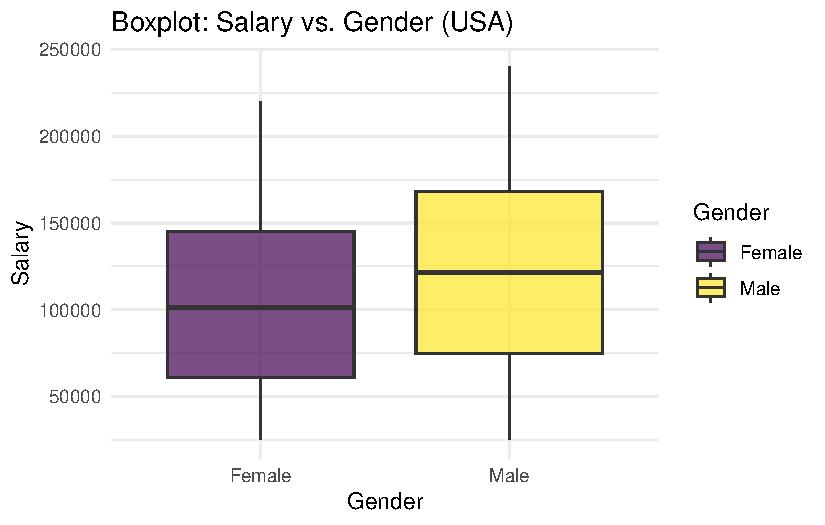
\includegraphics{main_doc_files/figure-pdf/unnamed-chunk-57-1.pdf}

}

\end{figure}

Nach intensiver Betrachtung der Grafiken bezüglich der Salary, kommt
folgende Frage auf:

Ist die Gender-Pay-Gap in China doch größer, da der größte Faktor für
die Salary die Years of Experience sind?

Hierzu werden die Korrelationen errechnet.

\hypertarget{korrelationen-zwischen-den-spalten}{%
\subsubsection{5.3.6 Korrelationen zwischen den
Spalten}\label{korrelationen-zwischen-den-spalten}}

\begin{Shaded}
\begin{Highlighting}[]
\NormalTok{correlation\_salary\_experience }\OtherTok{\textless{}{-}} \FunctionTok{cor}\NormalTok{(filtered\_data}\SpecialCharTok{$}\NormalTok{Salary, filtered\_data}\SpecialCharTok{$}\NormalTok{Years.Of.Experience)}

\FunctionTok{cat}\NormalTok{(}\StringTok{"Die Korrelation zwischen Salary und Years.Of.Experience ist:"}\NormalTok{, correlation\_salary\_experience, }\StringTok{"}\SpecialCharTok{\textbackslash{}n}\StringTok{"}\NormalTok{)}
\end{Highlighting}
\end{Shaded}

\begin{verbatim}
Die Korrelation zwischen Salary und Years.Of.Experience ist: 0.8103542 
\end{verbatim}

\begin{Shaded}
\begin{Highlighting}[]
\NormalTok{correlation\_salary\_education }\OtherTok{\textless{}{-}} \FunctionTok{cor}\NormalTok{(filtered\_data}\SpecialCharTok{$}\NormalTok{Salary, filtered\_data}\SpecialCharTok{$}\NormalTok{Education.Level, }\AttributeTok{use =} \StringTok{"complete.obs"}\NormalTok{)}

\FunctionTok{cat}\NormalTok{(}\StringTok{"Die Korrelation zwischen Salary und Education.Level ist:"}\NormalTok{, correlation\_salary\_education, }\StringTok{"}\SpecialCharTok{\textbackslash{}n}\StringTok{"}\NormalTok{)}
\end{Highlighting}
\end{Shaded}

\begin{verbatim}
Die Korrelation zwischen Salary und Education.Level ist: 0.6374551 
\end{verbatim}

\begin{Shaded}
\begin{Highlighting}[]
\NormalTok{correlation\_salary\_age }\OtherTok{\textless{}{-}} \FunctionTok{cor}\NormalTok{(filtered\_data}\SpecialCharTok{$}\NormalTok{Salary, filtered\_data}\SpecialCharTok{$}\NormalTok{Age, }\AttributeTok{use =} \StringTok{"complete.obs"}\NormalTok{)}

\FunctionTok{cat}\NormalTok{(}\StringTok{"Die Korrelation zwischen Salary und Age ist:"}\NormalTok{, correlation\_salary\_age, }\StringTok{"}\SpecialCharTok{\textbackslash{}n}\StringTok{"}\NormalTok{)}
\end{Highlighting}
\end{Shaded}

\begin{verbatim}
Die Korrelation zwischen Salary und Age ist: 0.7291603 
\end{verbatim}

\begin{Shaded}
\begin{Highlighting}[]
\NormalTok{correlation\_experience\_age }\OtherTok{\textless{}{-}} \FunctionTok{cor}\NormalTok{(filtered\_data}\SpecialCharTok{$}\NormalTok{Years.Of.Experience, filtered\_data}\SpecialCharTok{$}\NormalTok{Age, }\AttributeTok{use =} \StringTok{"complete.obs"}\NormalTok{)}

\FunctionTok{cat}\NormalTok{(}\StringTok{"Die Korrelation zwischen Years.Of.Experience und Age ist:"}\NormalTok{, correlation\_experience\_age, }\StringTok{"}\SpecialCharTok{\textbackslash{}n}\StringTok{"}\NormalTok{)}
\end{Highlighting}
\end{Shaded}

\begin{verbatim}
Die Korrelation zwischen Years.Of.Experience und Age ist: 0.9363709 
\end{verbatim}

\begin{Shaded}
\begin{Highlighting}[]
\NormalTok{correlation\_seniority\_experience }\OtherTok{\textless{}{-}} \FunctionTok{cor}\NormalTok{(filtered\_data}\SpecialCharTok{$}\NormalTok{Senior, filtered\_data}\SpecialCharTok{$}\NormalTok{Years.Of.Experience, }\AttributeTok{use =} \StringTok{"complete.obs"}\NormalTok{)}

\FunctionTok{cat}\NormalTok{(}\StringTok{"Die Korrelation zwischen Seniority und Years.Of.Experience ist:"}\NormalTok{, correlation\_seniority\_experience, }\StringTok{"}\SpecialCharTok{\textbackslash{}n}\StringTok{"}\NormalTok{)}
\end{Highlighting}
\end{Shaded}

\begin{verbatim}
Die Korrelation zwischen Seniority und Years.Of.Experience ist: 0.3192657 
\end{verbatim}

Das Ergebnis der Korrelationen:

\begin{itemize}
\item
  Von Salary und Years.of.experience ist es 0.81
\item
  Von Salary und Age ist es 0.73.
\item
  Von Age und Years.Of.Experience ist es 0.93.
\end{itemize}

Nun stellt sich folgende Frage:

Wie kommt es zu so einem großen Unterschied zwischen den Werten im
Vergleich zu Salary, obwohl sie doch eine starke Korrelation zueinander
haben?

Mögliche Antworten auf diese Frage wären:

Verteilung der Daten: Es ist möglich, dass die Verteilung der Daten in
den Variablen ``Age'' und ``Years.Of.Experience'' anders ist als in der
Variable ``Salary''. Wenn die Daten in ``Age'' und
``Years.Of.Experience'' breiter gestreut sind, kann dies zu einer
geringeren Korrelation führen, selbst wenn eine starke lineare Beziehung
besteht.

Nicht-lineare Beziehung: Die Korrelation misst nur lineare Beziehungen.
Wenn die Beziehung zwischen ``Age'' und ``Years.Of.Experience'' nicht
linear ist, könnte dies zu einem niedrigeren Korrelationswert führen.

Ausreißer: Das Vorhandensein von Ausreißern kann die Korrelation
beeinflussen. Wenn es Ausreißer in einer der Variablen gibt, kann dies
den Korrelationswert beeinträchtigen.

Stichprobengröße: Bei kleineren Stichproben können Korrelationswerte
instabiler sein.

Nun werden die Daten auf technische und administrative Jobs gefiltert,
anschließend werden die Gehälter der beiden Gruppen ausgegeben und in
einem Diagramm dargestellt und verglichen.

\begin{Shaded}
\begin{Highlighting}[]
\NormalTok{technische\_jobs }\OtherTok{\textless{}{-}} \FunctionTok{subset}\NormalTok{(filtered\_data, job\_type }\SpecialCharTok{==} \DecValTok{0}\NormalTok{)}
\NormalTok{admin\_jobs }\OtherTok{\textless{}{-}} \FunctionTok{subset}\NormalTok{(filtered\_data, job\_type }\SpecialCharTok{==} \DecValTok{1}\NormalTok{)}

\NormalTok{average\_salaries\_technical }\OtherTok{\textless{}{-}} \FunctionTok{mean}\NormalTok{(technische\_jobs}\SpecialCharTok{$}\NormalTok{Salary, }\AttributeTok{na.rm =} \ConstantTok{TRUE}\NormalTok{)}

\NormalTok{average\_salaries\_admin }\OtherTok{\textless{}{-}} \FunctionTok{mean}\NormalTok{(admin\_jobs}\SpecialCharTok{$}\NormalTok{Salary, }\AttributeTok{na.rm =} \ConstantTok{TRUE}\NormalTok{)}

\NormalTok{all\_average\_salaries }\OtherTok{\textless{}{-}} \FunctionTok{data.frame}\NormalTok{(}\AttributeTok{Job.Type =} \FunctionTok{c}\NormalTok{(}\StringTok{"technisch"}\NormalTok{, }\StringTok{"admin"}\NormalTok{),}
                                   \AttributeTok{Average.Salary =} \FunctionTok{c}\NormalTok{(average\_salaries\_technical, average\_salaries\_admin))}

\FunctionTok{ggplot}\NormalTok{(all\_average\_salaries, }\FunctionTok{aes}\NormalTok{(}\AttributeTok{x =}\NormalTok{ Job.Type, }\AttributeTok{y =}\NormalTok{ Average.Salary, }\AttributeTok{fill =}\NormalTok{ Job.Type)) }\SpecialCharTok{+}
  \FunctionTok{geom\_bar}\NormalTok{(}\AttributeTok{stat =} \StringTok{"identity"}\NormalTok{, }\AttributeTok{position =} \StringTok{"dodge"}\NormalTok{, }\AttributeTok{alpha =} \FloatTok{0.7}\NormalTok{) }\SpecialCharTok{+}
  \FunctionTok{scale\_fill\_viridis}\NormalTok{(}\AttributeTok{discrete =} \ConstantTok{TRUE}\NormalTok{) }\SpecialCharTok{+}
  \FunctionTok{labs}\NormalTok{(}\AttributeTok{title =} \StringTok{"Durchschnittliche Gehälter nach Jobtyp"}\NormalTok{,}
       \AttributeTok{x =} \StringTok{"Jobtyp"}\NormalTok{,}
       \AttributeTok{y =} \StringTok{"Durchschnittliches Gehalt"}\NormalTok{) }\SpecialCharTok{+}
  \FunctionTok{theme\_minimal}\NormalTok{() }\SpecialCharTok{+}
  \FunctionTok{scale\_y\_continuous}\NormalTok{(}\AttributeTok{labels =}\NormalTok{ scales}\SpecialCharTok{::}\NormalTok{comma)  }
\end{Highlighting}
\end{Shaded}

\begin{figure}[H]

{\centering 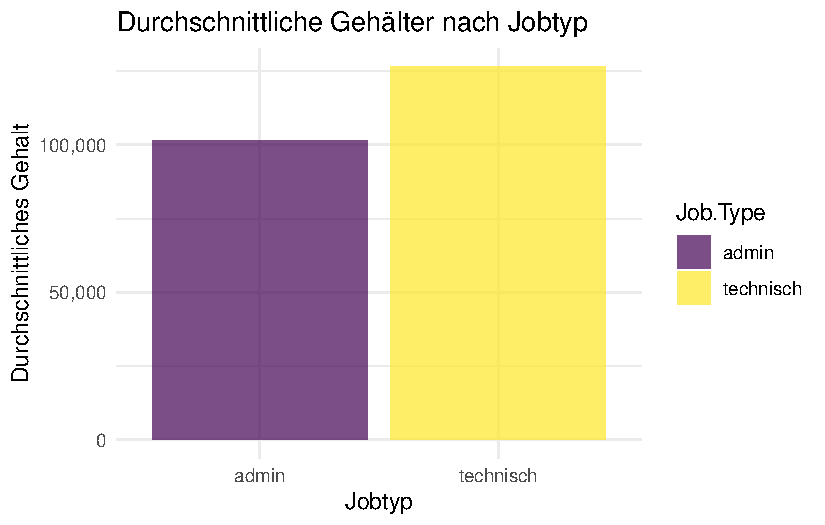
\includegraphics{main_doc_files/figure-pdf/unnamed-chunk-63-1.pdf}

}

\end{figure}

Obwohl in den administrativen Jobs auch Direktoren und Manager vertreten
sind, nehmen wir an, dass ein Manager einen Job Titel, wie ``Projekt
Manager'' und nicht ``Manager für Projekte'' hat und dieser Titel in
unserem Datensatz ``Director'' ist (Thema Führungsposition).

Unsere Untersuchungen haben ergeben, dass wir die Daten für unsere
Explorative Datenanalyse aber auch für die folgenden Regressionen neu
aufbereiten müssen.

Dazu werden folgende Fragen untersucht:

Unterscheidet sich ein Native und Expat im jeweiligen Land? Welche
Annahmen sind dafür nötig? Hier die Annahme das ``White'' generell nicht
ausgewandert ist, da wir hier Länder mit ähnlicher Kultur und Salary
haben.

\begin{Shaded}
\begin{Highlighting}[]
\FunctionTok{ggplot}\NormalTok{(filtered\_data, }\FunctionTok{aes}\NormalTok{(}\AttributeTok{x =}\NormalTok{ Country, }\AttributeTok{fill =}\NormalTok{ Race)) }\SpecialCharTok{+}
  \FunctionTok{geom\_bar}\NormalTok{(}\AttributeTok{position =} \StringTok{"dodge"}\NormalTok{) }\SpecialCharTok{+}
  \FunctionTok{scale\_fill\_viridis}\NormalTok{(}\AttributeTok{discrete =} \ConstantTok{TRUE}\NormalTok{) }\SpecialCharTok{+}
  \FunctionTok{labs}\NormalTok{(}\AttributeTok{title =} \StringTok{"Count of Races in Each Country"}\NormalTok{,}
       \AttributeTok{x =} \StringTok{"Country"}\NormalTok{,}
       \AttributeTok{y =} \StringTok{"Count"}\NormalTok{) }\SpecialCharTok{+}
  \FunctionTok{theme}\NormalTok{(}\AttributeTok{axis.text.x =} \FunctionTok{element\_text}\NormalTok{(}\AttributeTok{angle =} \DecValTok{45}\NormalTok{, }\AttributeTok{hjust =} \DecValTok{1}\NormalTok{))}
\end{Highlighting}
\end{Shaded}

\begin{figure}[H]

{\centering 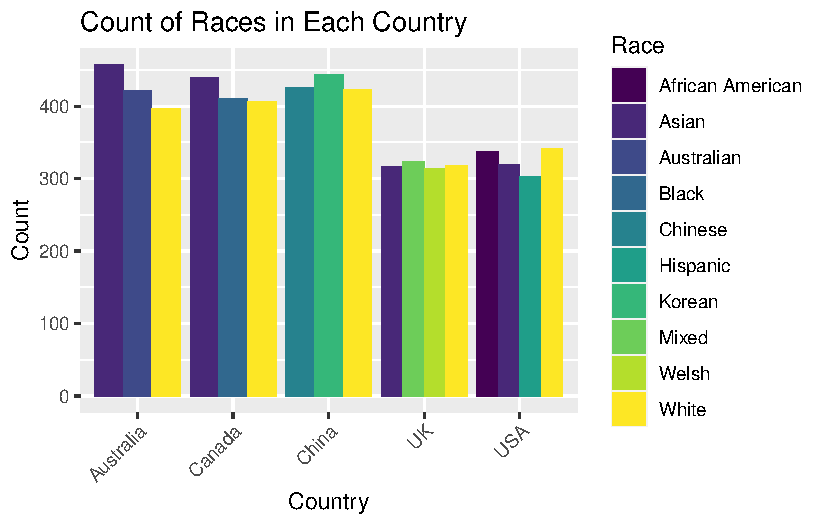
\includegraphics{main_doc_files/figure-pdf/unnamed-chunk-64-1.pdf}

}

\end{figure}

Dafür wird eine neue Spalte eingefügt, die mit numerischen Werten
arbeitet. 0 steht für Einheimische und 1 für einen Expat. Den Wert null
erhalten alle zeilen bei denen wir folgende Übereinstimmung feststellen:
African American (USA) White (Canada, USA, UK, Australia) Chinese
(China) Australian(Australia) Welsh (UK) jede andere Race ist
dementsprechend Expat und erhält eine 1 in der Spalte Expat.

\begin{Shaded}
\begin{Highlighting}[]
\NormalTok{filtered\_data}\SpecialCharTok{$}\NormalTok{Expat }\OtherTok{\textless{}{-}} \DecValTok{0}

\NormalTok{expat\_conditions }\OtherTok{\textless{}{-}} \FunctionTok{list}\NormalTok{(}
\NormalTok{  filtered\_data}\SpecialCharTok{$}\NormalTok{Race }\SpecialCharTok{==} \StringTok{"African American"} \SpecialCharTok{\&}\NormalTok{ filtered\_data}\SpecialCharTok{$}\NormalTok{Country }\SpecialCharTok{==} \StringTok{"USA"}\NormalTok{,}
\NormalTok{  filtered\_data}\SpecialCharTok{$}\NormalTok{Race }\SpecialCharTok{\%in\%} \FunctionTok{c}\NormalTok{(}\StringTok{"White"}\NormalTok{, }\StringTok{"Chinese"}\NormalTok{, }\StringTok{"Australian"}\NormalTok{, }\StringTok{"Welsh"}\NormalTok{) }\SpecialCharTok{\&}
\NormalTok{    filtered\_data}\SpecialCharTok{$}\NormalTok{Country }\SpecialCharTok{\%in\%} \FunctionTok{c}\NormalTok{(}\StringTok{"Canada"}\NormalTok{, }\StringTok{"USA"}\NormalTok{, }\StringTok{"UK"}\NormalTok{, }\StringTok{"Australia"}\NormalTok{),}
  \ConstantTok{TRUE}
\NormalTok{)}

\NormalTok{filtered\_data}\SpecialCharTok{$}\NormalTok{Expat }\OtherTok{\textless{}{-}} \FunctionTok{ifelse}\NormalTok{(expat\_conditions[[}\DecValTok{1}\NormalTok{]] }\SpecialCharTok{|}\NormalTok{ expat\_conditions[[}\DecValTok{2}\NormalTok{]], }\DecValTok{0}\NormalTok{, }
                               \FunctionTok{ifelse}\NormalTok{(expat\_conditions[[}\DecValTok{3}\NormalTok{]], }\DecValTok{1}\NormalTok{, }\ConstantTok{NA}\NormalTok{))}

\FunctionTok{head}\NormalTok{(filtered\_data)}
\end{Highlighting}
\end{Shaded}

\begin{verbatim}
# A tibble: 6 x 14
  Job.Title    job_count   Age Gender Education.Level Years.Of.Experience Salary
  <chr>            <int> <dbl> <chr>            <dbl>               <dbl>  <dbl>
1 Back end De~       242    33 Female               2                   5 110000
2 Back end De~       242    32 Male                 1                   4  95000
3 Back end De~       242    26 Female               2                   3  90000
4 Back end De~       242    26 Female               2                   2  70000
5 Back end De~       242    24 Female               1                   1  60000
6 Back end De~       242    26 Female               2                   3  90000
# i 7 more variables: Country <chr>, Race <chr>, Senior <dbl>, SalaryKat <fct>,
#   ID <int>, job_type <dbl>, Expat <dbl>
\end{verbatim}

Ausgabe hier sind nun die ersten Zeilen der aktualisierten Version von
``filtered\_data'', indem die Spalte ``Expat'' basierend auf den oben
genannten Kriterien befüllt wurde.

\hypertarget{thesen}{%
\section{6. Thesen}\label{thesen}}

Der folgende Absatz wird in unterschiedliche Teilabschnitte geteilt, um
eine gute Leserlichkeit zu erreichen.

Basierend auf den durchgeführten Tests und der Vorarbeit ergeben sich
folgende Thesen, die im Anschluss untersucht werden sollen:

\hypertarget{genderpaygap}{%
\subsection{6.1 Genderpaygap}\label{genderpaygap}}

\begin{enumerate}
\def\labelenumi{\arabic{enumi}.}
\tightlist
\item
  Männer verdienen mehr als Frauen.
\item
  Die Differenz der Salary zwischen den Geschlechtern ist in China höher
  als in den westlichen Ländern.
\item
  Männer haben im Durchschnitt mehr Years of Experience als Frauen
  -\textgreater{} Lässt sich die Genderpaygap auf die Yrs of Exp
  übertragen? Und gilt dies auch für China?
\end{enumerate}

\hypertarget{muxe4nner-verdienen-mehr-als-frauen}{%
\subsubsection{6.1.1 Männer verdienen mehr als
Frauen}\label{muxe4nner-verdienen-mehr-als-frauen}}

Zunächst stellt sich die Frage, ob Männer mehr verdienen als Frauen.
Hierzu wird ein Boxplot verwendet.

\begin{Shaded}
\begin{Highlighting}[]
\FunctionTok{ggplot}\NormalTok{(filtered\_data, }\FunctionTok{aes}\NormalTok{(}\AttributeTok{x =} \FunctionTok{factor}\NormalTok{(Gender), }\AttributeTok{y =}\NormalTok{ Salary, }\AttributeTok{fill =}\NormalTok{ Gender)) }\SpecialCharTok{+}
  \FunctionTok{geom\_boxplot}\NormalTok{(}\AttributeTok{alpha =} \FloatTok{0.7}\NormalTok{) }\SpecialCharTok{+}
  \FunctionTok{scale\_fill\_viridis}\NormalTok{(}\AttributeTok{discrete =} \ConstantTok{TRUE}\NormalTok{) }\SpecialCharTok{+}
  \FunctionTok{labs}\NormalTok{(}\AttributeTok{title =} \StringTok{"Boxplot: Salary vs. Gender"}\NormalTok{,}
       \AttributeTok{x =} \StringTok{"Gender"}\NormalTok{,}
       \AttributeTok{y =} \StringTok{"Salary"}\NormalTok{,}
       \AttributeTok{fill =} \StringTok{"Gender"}\NormalTok{) }\SpecialCharTok{+}
  \FunctionTok{theme\_minimal}\NormalTok{()}
\end{Highlighting}
\end{Shaded}

\begin{figure}[H]

{\centering 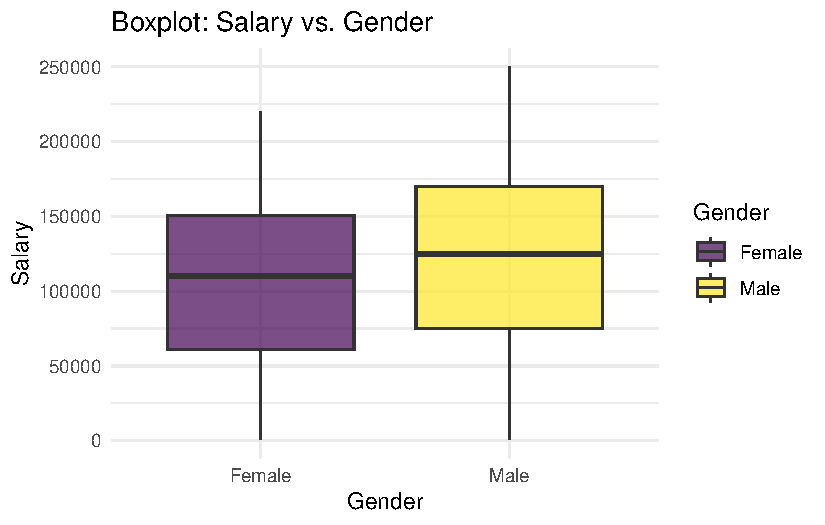
\includegraphics{main_doc_files/figure-pdf/unnamed-chunk-66-1.pdf}

}

\end{figure}

Anhand des Boxplots ist zu erkennen, dass der Median der Männer deutlich
höher, als der Median der Frauen ist. Aufgrund dieser Tatsache, lässt
sich sagen, dass diese Aussage korrekt ist.

\hypertarget{die-differenz-der-salary-zwischen-den-geschlechtern-ist-in-china-huxf6her-als-in-den-westlichen-luxe4ndern.-hier-alle-westlichen-luxe4nder-hinzufuxfcgen}{%
\subsubsection{6.1.2.: Die Differenz der Salary zwischen den
Geschlechtern ist in China höher als in den westlichen Ländern. Hier
alle westlichen Länder
hinzufügen}\label{die-differenz-der-salary-zwischen-den-geschlechtern-ist-in-china-huxf6her-als-in-den-westlichen-luxe4ndern.-hier-alle-westlichen-luxe4nder-hinzufuxfcgen}}

Um diese These zu beantworten werden zunächst die Erfahrungsjahre
zwischen China und den USA verglichen. Anschließend werden die Gehälter
verglichen. Nebenbei haben die Boxplots immer eine Differenzierung
zwischen Männern und Frauen um den Unterschied darzustellen.

Zu Beantwortung dieser These werden Boxplots verwendet.

\begin{Shaded}
\begin{Highlighting}[]
\NormalTok{data\_usa }\OtherTok{\textless{}{-}} \FunctionTok{subset}\NormalTok{(filtered\_data, Country }\SpecialCharTok{==} \StringTok{"USA"}\NormalTok{)}

\FunctionTok{ggplot}\NormalTok{(data\_usa, }\FunctionTok{aes}\NormalTok{(}\AttributeTok{x =} \FunctionTok{factor}\NormalTok{(Gender), }\AttributeTok{y =}\NormalTok{ Years.Of.Experience, }\AttributeTok{fill =}\NormalTok{ Gender)) }\SpecialCharTok{+}
  \FunctionTok{geom\_boxplot}\NormalTok{(}\AttributeTok{alpha =} \FloatTok{0.7}\NormalTok{) }\SpecialCharTok{+}
  \FunctionTok{scale\_fill\_viridis}\NormalTok{(}\AttributeTok{discrete =} \ConstantTok{TRUE}\NormalTok{) }\SpecialCharTok{+}
  \FunctionTok{labs}\NormalTok{(}\AttributeTok{title =} \StringTok{"Boxplot: Years of Experience vs. Gender (USA)"}\NormalTok{,}
       \AttributeTok{x =} \StringTok{"Gender"}\NormalTok{,}
       \AttributeTok{y =} \StringTok{"Years of Experience"}\NormalTok{,}
       \AttributeTok{fill =} \StringTok{"Gender"}\NormalTok{) }\SpecialCharTok{+}
  \FunctionTok{theme\_minimal}\NormalTok{()}
\end{Highlighting}
\end{Shaded}

\begin{figure}[H]

{\centering 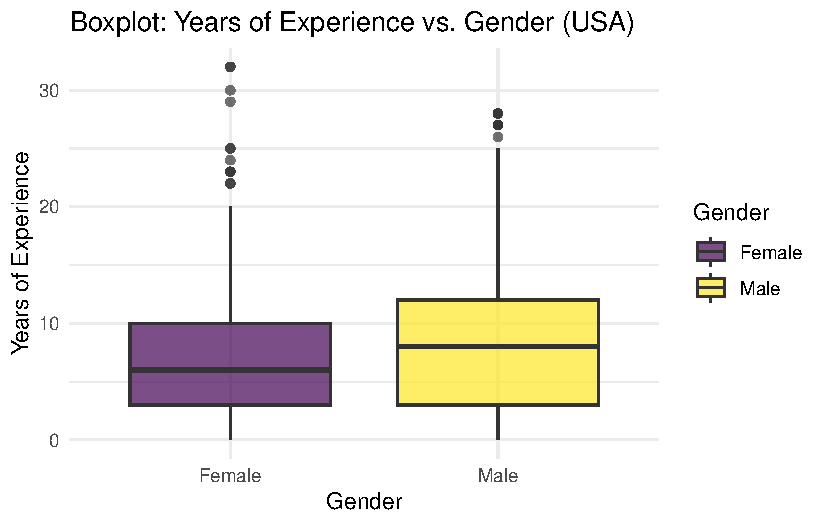
\includegraphics{main_doc_files/figure-pdf/unnamed-chunk-67-1.pdf}

}

\end{figure}

\begin{Shaded}
\begin{Highlighting}[]
\NormalTok{data\_china }\OtherTok{\textless{}{-}} \FunctionTok{subset}\NormalTok{(filtered\_data, Country }\SpecialCharTok{==} \StringTok{"China"}\NormalTok{)}

\FunctionTok{ggplot}\NormalTok{(data\_china, }\FunctionTok{aes}\NormalTok{(}\AttributeTok{x =} \FunctionTok{factor}\NormalTok{(Gender), }\AttributeTok{y =}\NormalTok{ Years.Of.Experience, }\AttributeTok{fill =}\NormalTok{ Gender)) }\SpecialCharTok{+}
  \FunctionTok{geom\_boxplot}\NormalTok{(}\AttributeTok{alpha =} \FloatTok{0.7}\NormalTok{) }\SpecialCharTok{+}
  \FunctionTok{scale\_fill\_viridis}\NormalTok{(}\AttributeTok{discrete =} \ConstantTok{TRUE}\NormalTok{) }\SpecialCharTok{+}
  \FunctionTok{labs}\NormalTok{(}\AttributeTok{title =} \StringTok{"Boxplot: Years of Experience vs. Gender (China)"}\NormalTok{,}
       \AttributeTok{x =} \StringTok{"Gender"}\NormalTok{,}
       \AttributeTok{y =} \StringTok{"Salary"}\NormalTok{,}
       \AttributeTok{fill =} \StringTok{"Gender"}\NormalTok{) }\SpecialCharTok{+}
  \FunctionTok{theme\_minimal}\NormalTok{()}
\end{Highlighting}
\end{Shaded}

\begin{figure}[H]

{\centering 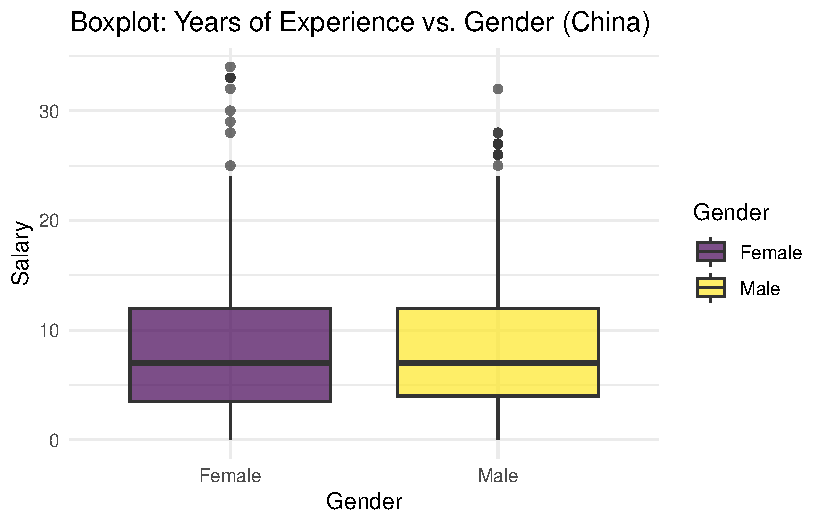
\includegraphics{main_doc_files/figure-pdf/unnamed-chunk-68-1.pdf}

}

\end{figure}

Anhand der ersten beiden Boxplots ist zu erkennen, dass Männer in der
USA deutlich mehr Berufserfahrung haben als Frauen. Wohin gegen der
Unterschied in China kaum zu erkennen ist.

\begin{Shaded}
\begin{Highlighting}[]
\NormalTok{data\_usa }\OtherTok{\textless{}{-}} \FunctionTok{subset}\NormalTok{(filtered\_data, Country }\SpecialCharTok{==} \StringTok{"USA"}\NormalTok{)}

\FunctionTok{ggplot}\NormalTok{(data\_usa, }\FunctionTok{aes}\NormalTok{(}\AttributeTok{x =} \FunctionTok{factor}\NormalTok{(Gender), }\AttributeTok{y =}\NormalTok{ Salary, }\AttributeTok{fill =}\NormalTok{ Gender)) }\SpecialCharTok{+}
  \FunctionTok{geom\_boxplot}\NormalTok{(}\AttributeTok{alpha =} \FloatTok{0.7}\NormalTok{) }\SpecialCharTok{+}
  \FunctionTok{scale\_fill\_viridis}\NormalTok{(}\AttributeTok{discrete =} \ConstantTok{TRUE}\NormalTok{) }\SpecialCharTok{+}
  \FunctionTok{labs}\NormalTok{(}\AttributeTok{title =} \StringTok{"Boxplot: Years of Experience vs. Gender (USA)"}\NormalTok{,}
       \AttributeTok{x =} \StringTok{"Gender"}\NormalTok{,}
       \AttributeTok{y =} \StringTok{"Years of Experience"}\NormalTok{,}
       \AttributeTok{fill =} \StringTok{"Gender"}\NormalTok{) }\SpecialCharTok{+}
  \FunctionTok{theme\_minimal}\NormalTok{()}
\end{Highlighting}
\end{Shaded}

\begin{figure}[H]

{\centering 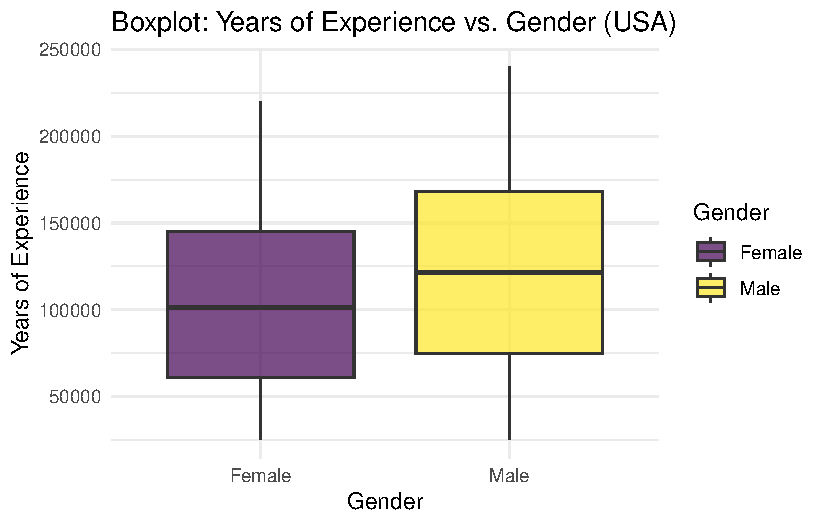
\includegraphics{main_doc_files/figure-pdf/unnamed-chunk-69-1.pdf}

}

\end{figure}

\begin{Shaded}
\begin{Highlighting}[]
\NormalTok{data\_china }\OtherTok{\textless{}{-}} \FunctionTok{subset}\NormalTok{(filtered\_data, Country }\SpecialCharTok{==} \StringTok{"China"}\NormalTok{)}

\FunctionTok{ggplot}\NormalTok{(data\_china, }\FunctionTok{aes}\NormalTok{(}\AttributeTok{x =} \FunctionTok{factor}\NormalTok{(Gender), }\AttributeTok{y =}\NormalTok{ Salary, }\AttributeTok{fill =}\NormalTok{ Gender)) }\SpecialCharTok{+}
  \FunctionTok{geom\_boxplot}\NormalTok{(}\AttributeTok{alpha =} \FloatTok{0.7}\NormalTok{) }\SpecialCharTok{+}
  \FunctionTok{scale\_fill\_viridis}\NormalTok{(}\AttributeTok{discrete =} \ConstantTok{TRUE}\NormalTok{) }\SpecialCharTok{+}
  \FunctionTok{labs}\NormalTok{(}\AttributeTok{title =} \StringTok{"Boxplot: Salary vs. Gender (China)"}\NormalTok{,}
       \AttributeTok{x =} \StringTok{"Gender"}\NormalTok{,}
       \AttributeTok{y =} \StringTok{"Salary"}\NormalTok{,}
       \AttributeTok{fill =} \StringTok{"Gender"}\NormalTok{) }\SpecialCharTok{+}
  \FunctionTok{theme\_minimal}\NormalTok{()}
\end{Highlighting}
\end{Shaded}

\begin{figure}[H]

{\centering 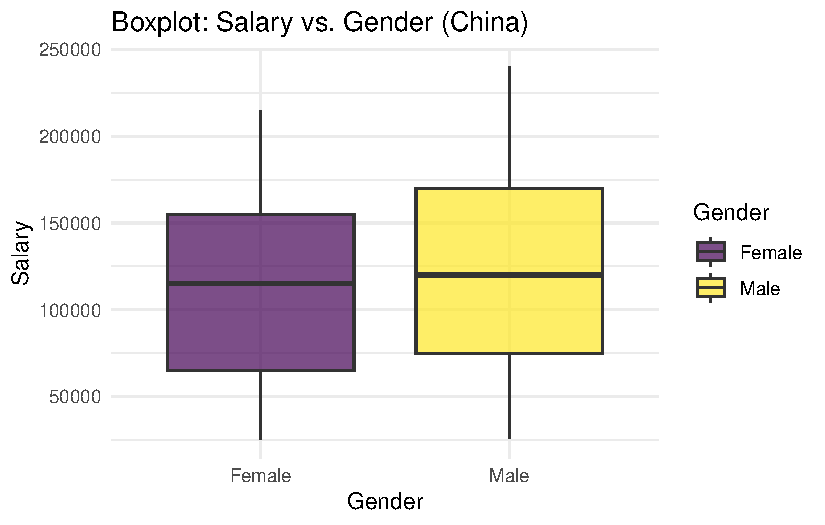
\includegraphics{main_doc_files/figure-pdf/unnamed-chunk-70-1.pdf}

}

\end{figure}

Durch die letzen beiden Boxplots ist zu erkennen, dass der Unterschied
im durchschnittlichen Gehalt in China und der USA mit dem bloßen Auge
nicht zu erkennen ist.\\
Unter Anbetracht der oberen beiden Boxplots ist jedoch, wie bereits
erwähnt, ein deutlicher Unterschied zwischen den Geschlechtern im Bezug
auf die Berufsaerfahrung zu erkennen.

\begin{Shaded}
\begin{Highlighting}[]
\NormalTok{correlation\_salary\_experience }\OtherTok{\textless{}{-}} \FunctionTok{cor}\NormalTok{(filtered\_data}\SpecialCharTok{$}\NormalTok{Salary, filtered\_data}\SpecialCharTok{$}\NormalTok{Years.Of.Experience)}

\FunctionTok{cat}\NormalTok{(}\StringTok{"Die Korrelation zwischen Salary und Years.Of.Experience ist:"}\NormalTok{, correlation\_salary\_experience, }\StringTok{"}\SpecialCharTok{\textbackslash{}n}\StringTok{"}\NormalTok{)}
\end{Highlighting}
\end{Shaded}

\begin{verbatim}
Die Korrelation zwischen Salary und Years.Of.Experience ist: 0.8103542 
\end{verbatim}

Aus den obigen Tests ist außerdem hervorgegangen, dass die
Berufserfahrung eine hohe Korrelation zu dem Gehalt hat.

Deswegen lässt sich trotzdem sagen, dass diese These korrekt ist.

\hypertarget{muxe4nner-haben-im-durchschnitt-mehr-berufserfahrung-als-frauen}{%
\subsubsection{6.1.3.: Männer haben im Durchschnitt mehr Berufserfahrung
als
Frauen}\label{muxe4nner-haben-im-durchschnitt-mehr-berufserfahrung-als-frauen}}

\begin{Shaded}
\begin{Highlighting}[]
\FunctionTok{ggplot}\NormalTok{(filtered\_data, }\FunctionTok{aes}\NormalTok{(}\AttributeTok{x =} \FunctionTok{factor}\NormalTok{(Gender), }\AttributeTok{y =}\NormalTok{ Years.Of.Experience, }\AttributeTok{fill =}\NormalTok{ Gender)) }\SpecialCharTok{+}
  \FunctionTok{geom\_boxplot}\NormalTok{(}\AttributeTok{alpha =} \FloatTok{0.7}\NormalTok{) }\SpecialCharTok{+}
  \FunctionTok{scale\_fill\_viridis}\NormalTok{(}\AttributeTok{discrete =} \ConstantTok{TRUE}\NormalTok{) }\SpecialCharTok{+}
  \FunctionTok{labs}\NormalTok{(}\AttributeTok{title =} \StringTok{"Boxplot: Years of Experience vs. Gender"}\NormalTok{,}
       \AttributeTok{x =} \StringTok{"Gender"}\NormalTok{,}
       \AttributeTok{y =} \StringTok{"Years of Experience"}\NormalTok{,}
       \AttributeTok{fill =} \StringTok{"Gender"}\NormalTok{) }\SpecialCharTok{+}
  \FunctionTok{theme\_minimal}\NormalTok{()}
\end{Highlighting}
\end{Shaded}

\begin{figure}[H]

{\centering 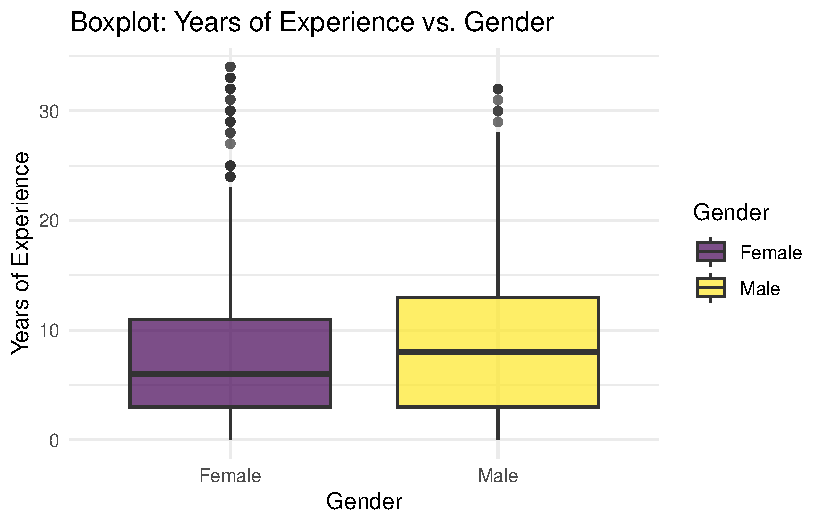
\includegraphics{main_doc_files/figure-pdf/unnamed-chunk-72-1.pdf}

}

\end{figure}

Die These ist korrekt, wie anhand des obigen Boxplots zu erkennen ist.
Der Median liegt bei den Männern höher, als bei den Frauen.

\hypertarget{zugewanderte-menschen-verdienen-mehr-als-einheimische-menschen}{%
\subsection{6.2 Zugewanderte Menschen verdienen mehr als einheimische
Menschen}\label{zugewanderte-menschen-verdienen-mehr-als-einheimische-menschen}}

Unsere Untersuchungen haben ergeben, dass wir die Daten für unsere
Explorative Datenanalyse, sowie auch die Regression neu aufbereiten
müssen.

Dazu untersuchen wir:

Wie unterscheide ich einen Native und Expat im jeweiligen Land. Welche
Annahmen sind dafür nötig? Hier die Annahme, dass ``White'' generell
nicht ausgewandert ist, da der Datensatz Länder mit ähnlicher Kultur und
Salary beinhaltet.

\hypertarget{alle-ethnizituxe4ten-je-land}{%
\subsubsection{6.2.1.: Alle Ethnizitäten je
Land}\label{alle-ethnizituxe4ten-je-land}}

\begin{Shaded}
\begin{Highlighting}[]
\FunctionTok{ggplot}\NormalTok{(filtered\_data, }\FunctionTok{aes}\NormalTok{(}\AttributeTok{x =}\NormalTok{ Country, }\AttributeTok{fill =}\NormalTok{ Race)) }\SpecialCharTok{+}
  \FunctionTok{geom\_bar}\NormalTok{(}\AttributeTok{position =} \StringTok{"dodge"}\NormalTok{) }\SpecialCharTok{+}
  \FunctionTok{scale\_fill\_viridis}\NormalTok{(}\AttributeTok{discrete =} \ConstantTok{TRUE}\NormalTok{) }\SpecialCharTok{+}
  \FunctionTok{labs}\NormalTok{(}\AttributeTok{title =} \StringTok{"Count of Races in Each Country"}\NormalTok{,}
       \AttributeTok{x =} \StringTok{"Country"}\NormalTok{,}
       \AttributeTok{y =} \StringTok{"Count"}\NormalTok{) }\SpecialCharTok{+}
  \FunctionTok{theme}\NormalTok{(}\AttributeTok{axis.text.x =} \FunctionTok{element\_text}\NormalTok{(}\AttributeTok{angle =} \DecValTok{45}\NormalTok{, }\AttributeTok{hjust =} \DecValTok{1}\NormalTok{))}
\end{Highlighting}
\end{Shaded}

\begin{figure}[H]

{\centering 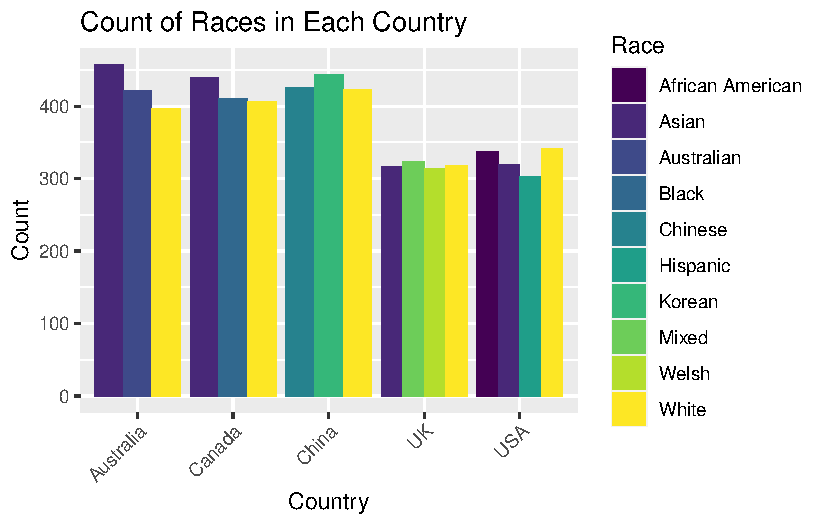
\includegraphics{main_doc_files/figure-pdf/unnamed-chunk-73-1.pdf}

}

\end{figure}

Hier ist ist zu erkennen, welche Ethnizitäten in den unterschiedlichen
Ländern existieren. So ist zu erkennen, dass es nie mehr als vier
Ethnizitäten pro Land gibt.

\hypertarget{gesamtbetrachtung}{%
\subsubsection{6.2.2.: Gesamtbetrachtung}\label{gesamtbetrachtung}}

\begin{Shaded}
\begin{Highlighting}[]
\FunctionTok{ggplot}\NormalTok{(filtered\_data, }\FunctionTok{aes}\NormalTok{(}\AttributeTok{x =} \FunctionTok{as.factor}\NormalTok{(Expat), }\AttributeTok{y =}\NormalTok{ Salary, }\AttributeTok{fill =} \FunctionTok{factor}\NormalTok{(Expat))) }\SpecialCharTok{+}
  \FunctionTok{geom\_boxplot}\NormalTok{() }\SpecialCharTok{+}
  \FunctionTok{scale\_fill\_viridis}\NormalTok{(}\AttributeTok{discrete =} \ConstantTok{TRUE}\NormalTok{) }\SpecialCharTok{+}
  \FunctionTok{labs}\NormalTok{(}\AttributeTok{title =} \StringTok{"Vergleich der Gehälter von Zugewanderten und Einheimischen"}\NormalTok{,}
       \AttributeTok{x =} \StringTok{"Expat"}\NormalTok{,}
       \AttributeTok{y =} \StringTok{"Gehalt"}\NormalTok{) }\SpecialCharTok{+}
  \FunctionTok{scale\_x\_discrete}\NormalTok{(}\AttributeTok{labels =} \FunctionTok{c}\NormalTok{(}\StringTok{"Einheimische (0)"}\NormalTok{, }\StringTok{"Zugewanderte (1)"}\NormalTok{)) }\SpecialCharTok{+}
  \FunctionTok{theme\_minimal}\NormalTok{()}
\end{Highlighting}
\end{Shaded}

\begin{figure}[H]

{\centering 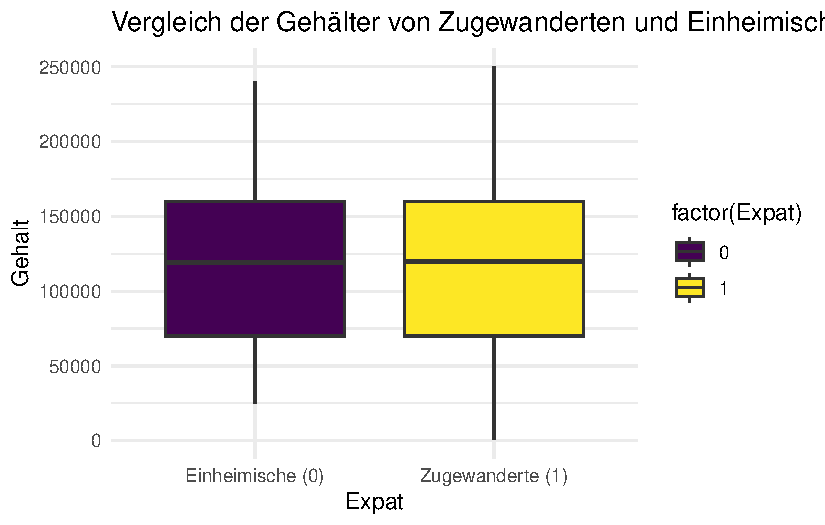
\includegraphics{main_doc_files/figure-pdf/unnamed-chunk-74-1.pdf}

}

\end{figure}

Aus diesem Diagramm geht hervor, dass vorerst kein Unterschied zu
erkennen ist.

\begin{Shaded}
\begin{Highlighting}[]
\NormalTok{mean\_salary\_expat }\OtherTok{\textless{}{-}} \FunctionTok{mean}\NormalTok{(filtered\_data}\SpecialCharTok{$}\NormalTok{Salary[filtered\_data}\SpecialCharTok{$}\NormalTok{Expat }\SpecialCharTok{==} \DecValTok{1}\NormalTok{], }\AttributeTok{na.rm =} \ConstantTok{TRUE}\NormalTok{)}
\NormalTok{mean\_salary\_expat}
\end{Highlighting}
\end{Shaded}

\begin{verbatim}
[1] 116928.1
\end{verbatim}

\begin{Shaded}
\begin{Highlighting}[]
\NormalTok{mean\_salary\_native }\OtherTok{\textless{}{-}} \FunctionTok{mean}\NormalTok{(filtered\_data}\SpecialCharTok{$}\NormalTok{Salary[filtered\_data}\SpecialCharTok{$}\NormalTok{Expat }\SpecialCharTok{==} \DecValTok{0}\NormalTok{], }\AttributeTok{na.rm =} \ConstantTok{TRUE}\NormalTok{)}
\NormalTok{mean\_salary\_native}
\end{Highlighting}
\end{Shaded}

\begin{verbatim}
[1] 116572.5
\end{verbatim}

Auch nach Darstellung der Mittelwerte ist kein wirklicher Unterschied zu
erkennen.

Deswegen wird die These verworfen, da es offensichtlich keine
Unterschiede gibt.

\hypertarget{gibt-es-einen-unterschied-im-gehalt-zwischen-den-verschiedenen-bildungsniveaus}{%
\subsection{6.3 Gibt es einen Unterschied im Gehalt zwischen den
verschiedenen
Bildungsniveaus?}\label{gibt-es-einen-unterschied-im-gehalt-zwischen-den-verschiedenen-bildungsniveaus}}

Vorab muss erwähnt werden, dass ohne ein Mindestmaß an Bildung keine
weitere Gehaltsentwicklung möglich ist.

Das sind die Bedeutungen der verschiedenen Bildungsniveaus:

0 = High School Abschluss

1 = Bachelor

2 = Master

3 = Doctor

Um diese These zu beantworten sind wir auf verschiedene Lösungsansätze
gekommen, die uns helfen könnten:

\begin{enumerate}
\def\labelenumi{\arabic{enumi}.}
\item
  \textbf{Deskriptive Statistiken:} Es könnten Quantile oder Perzentile
  des Gehalts für jeden Bildungsniveau berechnet berechnet werden. Dies
  könnte einen Überblick über die Verteilung der Gehälter bieten und
  zeigt potenzielle Grenzwerte.
\item
  \textbf{Boxplots pro Bildungsniveau:} Es könnten Boxplots für jedes
  Bildungsniveau erstellt werden, um die Verteilung der Gehälter visuell
  zu vergleichen. Dies könnte unterstützend wirken, um Ausreißer und
  Unterschiede im Bildungsniveau zu identifizieren.
\item
  \textbf{Visualisierungen:} Es besteht die Möglichkeit verschiedene
  Visualiersierungen, wie Scatterplots oder Liniendiagramme zu
  erstellen, um Trends oder Muster zwischen Gehalt und Bildungsniveau zu
  erkennen.
\end{enumerate}

\hypertarget{desktiptive-statistiken}{%
\subsubsection{6.3.1.: Desktiptive
Statistiken:}\label{desktiptive-statistiken}}

Hierzu werden erst die Daten berechnet und diese anschließend für die
Grafik ``ge-reshaped''.

\begin{Shaded}
\begin{Highlighting}[]
\FunctionTok{library}\NormalTok{(ggplot2)}
\FunctionTok{library}\NormalTok{(dplyr)}

\CommentTok{\# Daten berechnen}
\NormalTok{salary\_percentiles }\OtherTok{\textless{}{-}}\NormalTok{ filtered\_data }\SpecialCharTok{\%\textgreater{}\%}
  \FunctionTok{group\_by}\NormalTok{(Education.Level) }\SpecialCharTok{\%\textgreater{}\%}
  \FunctionTok{summarise}\NormalTok{(}\StringTok{\textasciigrave{}}\AttributeTok{10th Percentile}\StringTok{\textasciigrave{}} \OtherTok{=} \FunctionTok{quantile}\NormalTok{(Salary, }\AttributeTok{probs =} \FloatTok{0.1}\NormalTok{, }\AttributeTok{na.rm =} \ConstantTok{TRUE}\NormalTok{),}
            \StringTok{\textasciigrave{}}\AttributeTok{25th Percentile}\StringTok{\textasciigrave{}} \OtherTok{=} \FunctionTok{quantile}\NormalTok{(Salary, }\AttributeTok{probs =} \FloatTok{0.25}\NormalTok{, }\AttributeTok{na.rm =} \ConstantTok{TRUE}\NormalTok{),}
            \StringTok{\textasciigrave{}}\AttributeTok{50th Percentile (Median)}\StringTok{\textasciigrave{}} \OtherTok{=} \FunctionTok{quantile}\NormalTok{(Salary, }\AttributeTok{probs =} \FloatTok{0.5}\NormalTok{, }\AttributeTok{na.rm =} \ConstantTok{TRUE}\NormalTok{),}
            \StringTok{\textasciigrave{}}\AttributeTok{75th Percentile}\StringTok{\textasciigrave{}} \OtherTok{=} \FunctionTok{quantile}\NormalTok{(Salary, }\AttributeTok{probs =} \FloatTok{0.75}\NormalTok{, }\AttributeTok{na.rm =} \ConstantTok{TRUE}\NormalTok{),}
            \StringTok{\textasciigrave{}}\AttributeTok{90th Percentile}\StringTok{\textasciigrave{}} \OtherTok{=} \FunctionTok{quantile}\NormalTok{(Salary, }\AttributeTok{probs =} \FloatTok{0.9}\NormalTok{, }\AttributeTok{na.rm =} \ConstantTok{TRUE}\NormalTok{))}

\NormalTok{salary\_percentiles\_long }\OtherTok{\textless{}{-}}\NormalTok{ salary\_percentiles }\SpecialCharTok{\%\textgreater{}\%}
\NormalTok{  tidyr}\SpecialCharTok{::}\FunctionTok{pivot\_longer}\NormalTok{(}\AttributeTok{cols =} \SpecialCharTok{{-}}\NormalTok{Education.Level, }\AttributeTok{names\_to =} \StringTok{"Percentile"}\NormalTok{, }\AttributeTok{values\_to =} \StringTok{"Salary"}\NormalTok{)}

\FunctionTok{ggplot}\NormalTok{(salary\_percentiles\_long, }\FunctionTok{aes}\NormalTok{(}\AttributeTok{x =}\NormalTok{ Education.Level, }\AttributeTok{y =}\NormalTok{ Salary, }\AttributeTok{fill =}\NormalTok{ Percentile)) }\SpecialCharTok{+}
  \FunctionTok{geom\_bar}\NormalTok{(}\AttributeTok{stat =} \StringTok{"identity"}\NormalTok{, }\AttributeTok{position =} \StringTok{"dodge"}\NormalTok{, }\AttributeTok{alpha =} \FloatTok{0.7}\NormalTok{) }\SpecialCharTok{+}
  \FunctionTok{scale\_fill\_viridis}\NormalTok{(}\AttributeTok{discrete =} \ConstantTok{TRUE}\NormalTok{) }\SpecialCharTok{+}
  \FunctionTok{labs}\NormalTok{(}\AttributeTok{title =} \StringTok{"Perzentile des Gehalts nach Bildungsniveau"}\NormalTok{,}
       \AttributeTok{x =} \StringTok{"Bildungsniveau"}\NormalTok{,}
       \AttributeTok{y =} \StringTok{"Gehalt"}\NormalTok{,}
       \AttributeTok{fill =} \StringTok{"Perzentil"}\NormalTok{) }\SpecialCharTok{+}
  \FunctionTok{theme\_minimal}\NormalTok{()}
\end{Highlighting}
\end{Shaded}

\begin{figure}[H]

{\centering 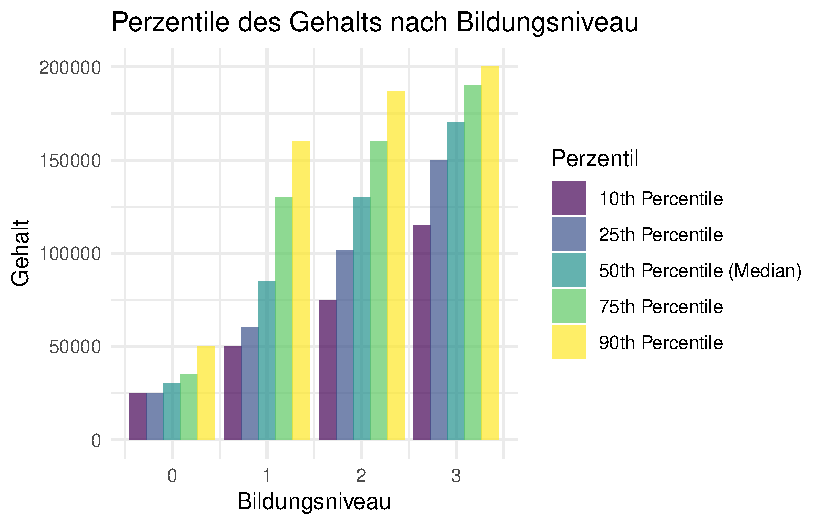
\includegraphics{main_doc_files/figure-pdf/unnamed-chunk-76-1.pdf}

}

\end{figure}

In dem gruppierten Balkendiagramm kann erkannt werden, dass die
unterschiedlichen Perzentile stets mit dem Bildungsniveau zusammen
ansteigen.

\begin{Shaded}
\begin{Highlighting}[]
\NormalTok{average\_salary\_education }\OtherTok{\textless{}{-}} \FunctionTok{aggregate}\NormalTok{(Salary }\SpecialCharTok{\textasciitilde{}}\NormalTok{ Education.Level, }\AttributeTok{data =}\NormalTok{ filtered\_data, }\AttributeTok{FUN =}\NormalTok{ mean, }\AttributeTok{na.rm =} \ConstantTok{TRUE}\NormalTok{)}

\NormalTok{average\_salary\_education}
\end{Highlighting}
\end{Shaded}

\begin{verbatim}
  Education.Level    Salary
1               0  34511.62
2               1  97042.04
3               2 129983.77
4               3 165796.75
\end{verbatim}

Die oben gestellte Aussage wird erneut bestätigt, durch die Ausgabe der
``Average Salary''. Hier ist zu erkennen, dass das durchschnittliche
Gehalt höher ist, je höher das Bildungsniveau ist.

\hypertarget{boxplots-pro-bildungsniveau}{%
\subsubsection{\texorpdfstring{6.3.2.: \textbf{Boxplots pro
Bildungsniveau:}}{6.3.2.: Boxplots pro Bildungsniveau:}}\label{boxplots-pro-bildungsniveau}}

\begin{Shaded}
\begin{Highlighting}[]
\NormalTok{filtered\_data }\OtherTok{\textless{}{-}}\NormalTok{ filtered\_data }\SpecialCharTok{\%\textgreater{}\%}
  \FunctionTok{mutate}\NormalTok{(}\AttributeTok{Education.Level =} \FunctionTok{factor}\NormalTok{(Education.Level, }\AttributeTok{levels =} \FunctionTok{unique}\NormalTok{(}\FunctionTok{sort}\NormalTok{(Education.Level))))}

\FunctionTok{ggplot}\NormalTok{(filtered\_data, }\FunctionTok{aes}\NormalTok{(}\AttributeTok{x =} \FunctionTok{reorder}\NormalTok{(}\FunctionTok{factor}\NormalTok{(Education.Level), Salary, }\AttributeTok{FUN =}\NormalTok{ median), }\AttributeTok{y =}\NormalTok{ Salary)) }\SpecialCharTok{+}
  \FunctionTok{geom\_boxplot}\NormalTok{(}\AttributeTok{color =} \StringTok{"black"}\NormalTok{, }\AttributeTok{fill =} \FunctionTok{viridis}\NormalTok{(}\DecValTok{2}\NormalTok{)[}\DecValTok{2}\NormalTok{]) }\SpecialCharTok{+}
  \FunctionTok{labs}\NormalTok{(}\AttributeTok{title =} \StringTok{"Boxplot des Gehalts nach Bildungsniveau"}\NormalTok{,}
       \AttributeTok{x =} \StringTok{"Bildungsniveau"}\NormalTok{,}
       \AttributeTok{y =} \StringTok{"Gehalt"}\NormalTok{) }\SpecialCharTok{+}
  \FunctionTok{theme\_minimal}\NormalTok{()}
\end{Highlighting}
\end{Shaded}

\begin{figure}[H]

{\centering 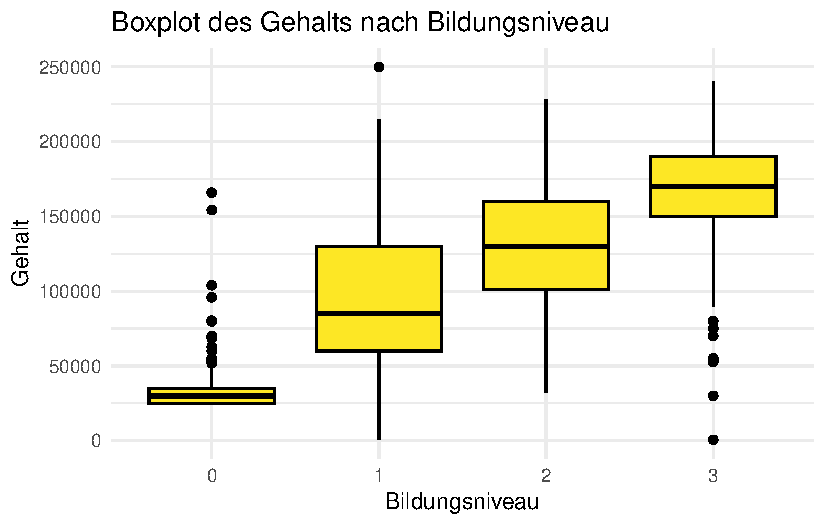
\includegraphics{main_doc_files/figure-pdf/unnamed-chunk-78-1.pdf}

}

\end{figure}

Auch in dem Balkendiagramm ist, genau wie oben, zu erkennen, dass der
Median stets höher ist, je höher das Bildungsniveau geht.

\hypertarget{visualisierungen}{%
\subsubsection{\texorpdfstring{6.3.3.:
\textbf{Visualisierungen:}}{6.3.3.: Visualisierungen:}}\label{visualisierungen}}

\begin{Shaded}
\begin{Highlighting}[]
\NormalTok{filtered\_data }\OtherTok{\textless{}{-}}\NormalTok{ filtered\_data }\SpecialCharTok{\%\textgreater{}\%}
  \FunctionTok{mutate}\NormalTok{(}\AttributeTok{Education.Level =} \FunctionTok{factor}\NormalTok{(Education.Level, }\AttributeTok{levels =} \FunctionTok{unique}\NormalTok{(}\FunctionTok{sort}\NormalTok{(Education.Level))))}

\FunctionTok{ggplot}\NormalTok{(filtered\_data, }\FunctionTok{aes}\NormalTok{(}\AttributeTok{x =} \FunctionTok{reorder}\NormalTok{(}\FunctionTok{factor}\NormalTok{(Education.Level), Salary, }\AttributeTok{FUN =}\NormalTok{ median), }\AttributeTok{y =}\NormalTok{ Salary)) }\SpecialCharTok{+}
  \FunctionTok{geom\_point}\NormalTok{() }\SpecialCharTok{+} 
  \FunctionTok{scale\_fill\_viridis}\NormalTok{(}\AttributeTok{discrete =} \ConstantTok{TRUE}\NormalTok{) }\SpecialCharTok{+}
  \FunctionTok{labs}\NormalTok{(}\AttributeTok{title =} \StringTok{"Gehalt nach Bildungslevel"}\NormalTok{,}
       \AttributeTok{x =} \StringTok{"Bildungslevel"}\NormalTok{,}
       \AttributeTok{y =} \StringTok{"Gehalt"}\NormalTok{) }\SpecialCharTok{+}
  \FunctionTok{theme\_minimal}\NormalTok{()}
\end{Highlighting}
\end{Shaded}

\begin{figure}[H]

{\centering 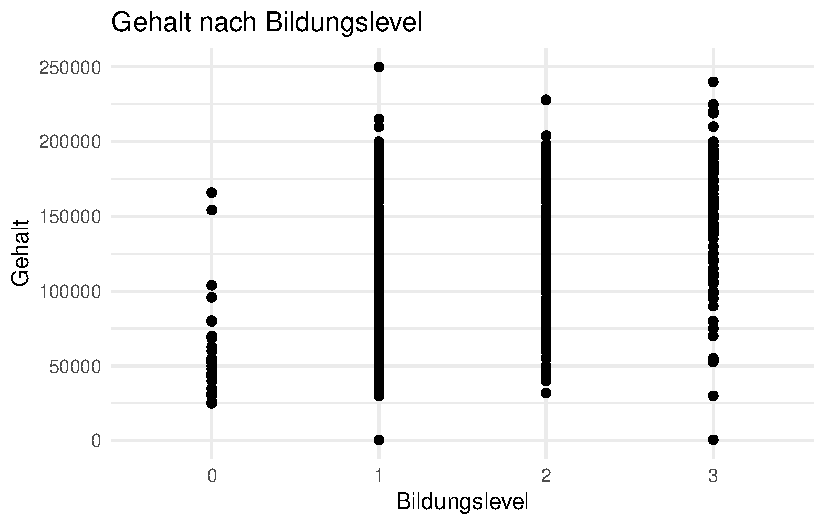
\includegraphics{main_doc_files/figure-pdf/unnamed-chunk-79-1.pdf}

}

\end{figure}

Der folgende Code erstellt ein Liniendiagramm, dass das Gehalt in
Abhängigkeit vom Bildungsniveau darstellt. Zunächst wird das
Bildungsniveau neu angeordnet und danach das Liniendiagramm erstellt.

\begin{Shaded}
\begin{Highlighting}[]
\NormalTok{filtered\_data}\SpecialCharTok{$}\NormalTok{Education.Level }\OtherTok{\textless{}{-}} \FunctionTok{factor}\NormalTok{(filtered\_data}\SpecialCharTok{$}\NormalTok{Education.Level, }\AttributeTok{levels =} \FunctionTok{c}\NormalTok{(}\StringTok{"0"}\NormalTok{, }\StringTok{"1"}\NormalTok{, }\StringTok{"2"}\NormalTok{, }\StringTok{"3"}\NormalTok{))}

\FunctionTok{ggplot}\NormalTok{(filtered\_data, }\FunctionTok{aes}\NormalTok{(}\AttributeTok{x =}\NormalTok{ Education.Level, }\AttributeTok{y =}\NormalTok{ Salary, }\AttributeTok{group =} \DecValTok{1}\NormalTok{)) }\SpecialCharTok{+}
  \FunctionTok{geom\_line}\NormalTok{() }\SpecialCharTok{+}
  \FunctionTok{stat\_summary}\NormalTok{(}\AttributeTok{fun.y =}\NormalTok{ median, }\AttributeTok{geom =} \StringTok{"point"}\NormalTok{, }\AttributeTok{size =} \DecValTok{3}\NormalTok{, }\AttributeTok{color =} \StringTok{"red"}\NormalTok{) }\SpecialCharTok{+}
  \FunctionTok{labs}\NormalTok{(}\AttributeTok{title =} \StringTok{"Gehalt nach Bildungslevel"}\NormalTok{,}
       \AttributeTok{x =} \StringTok{"Bildungslevel"}\NormalTok{,}
       \AttributeTok{y =} \StringTok{"Gehalt"}\NormalTok{) }\SpecialCharTok{+}
  \FunctionTok{theme\_minimal}\NormalTok{()}
\end{Highlighting}
\end{Shaded}

\begin{verbatim}
Warning: The `fun.y` argument of `stat_summary()` is deprecated as of ggplot2 3.3.0.
i Please use the `fun` argument instead.
\end{verbatim}

\begin{figure}[H]

{\centering 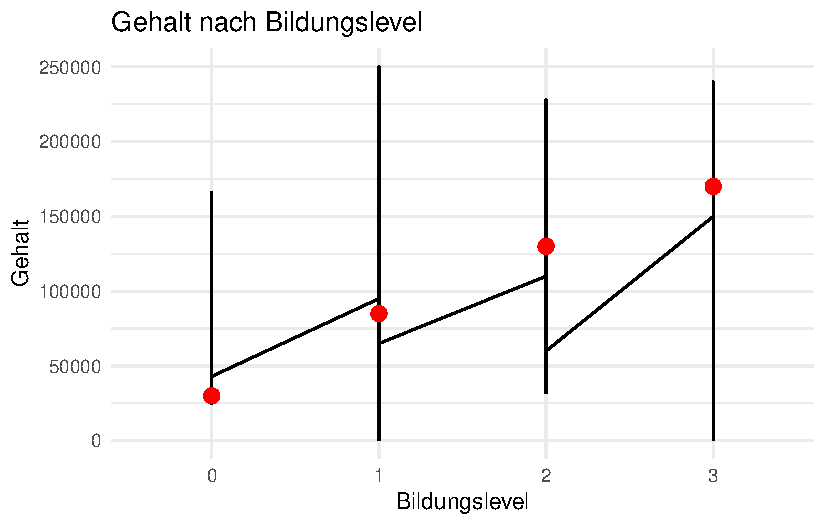
\includegraphics{main_doc_files/figure-pdf/unnamed-chunk-80-1.pdf}

}

\end{figure}

Die roten Punkte zeigen den Medianwert des Gehalts je nach
Bildungsniveau. Die schrägen Linien zeigen den Trend steigender Gehälter
bei höheren Bildungsstufen.

Ohne einen Hochschulabschluss gibt es eine Gehaltsgrenze. Die Top 90\%
ohne Hochschulabschluss fangen bei den unteren 10\% mit
Hochschulabschluss an aus der Sicht des Gehalts.

Die These kann als Korrekt angesehen werden, da alle Lösungsansätze im
Allgemeinen, das gleiche Ergebnis liefern.

\hypertarget{die-technischen-jobs-haben-ein-huxf6heres-gehalt-als-die-administrativen-jobs}{%
\subsection{6.4 Die technischen Jobs haben ein höheres Gehalt als die
administrativen
Jobs}\label{die-technischen-jobs-haben-ein-huxf6heres-gehalt-als-die-administrativen-jobs}}

\hypertarget{daten-aufbereiten-1}{%
\subsubsection{6.4.1.: Daten Aufbereiten}\label{daten-aufbereiten-1}}

Unter dem Punkt ``Daten aufbereiten 2'' wurden bereits alle Jobs in
administrativ und technisch unterteilt.

Zudem werden noch im folgenden alle Werte aus dem Datensatz gefiltert,
die den Jobtitel ``Director'' enthalten, da dieser Job nicht eindeutig
einer Gruppe zugeordnet werden kann (z.B ``Engineering Director'').

\begin{Shaded}
\begin{Highlighting}[]
\NormalTok{filtered\_data2 }\OtherTok{\textless{}{-}}\NormalTok{ filtered\_data}

\NormalTok{director\_jobs }\OtherTok{\textless{}{-}}\NormalTok{ filtered\_data2 }\SpecialCharTok{\%\textgreater{}\%}
  \FunctionTok{filter}\NormalTok{(}\FunctionTok{grepl}\NormalTok{(}\StringTok{"Director"}\NormalTok{, Job.Title))}

\NormalTok{filtered\_data2 }\OtherTok{\textless{}{-}}\NormalTok{ filtered\_data2 }\SpecialCharTok{\%\textgreater{}\%}
  \FunctionTok{anti\_join}\NormalTok{(director\_jobs)}
\end{Highlighting}
\end{Shaded}

\begin{verbatim}
Joining with `by = join_by(Job.Title, job_count, Age, Gender, Education.Level,
Years.Of.Experience, Salary, Country, Race, Senior, SalaryKat, ID, job_type,
Expat)`
\end{verbatim}

\begin{Shaded}
\begin{Highlighting}[]
\FunctionTok{nrow}\NormalTok{(director\_jobs)}
\end{Highlighting}
\end{Shaded}

\begin{verbatim}
[1] 416
\end{verbatim}

\begin{Shaded}
\begin{Highlighting}[]
\FunctionTok{nrow}\NormalTok{(filtered\_data)}
\end{Highlighting}
\end{Shaded}

\begin{verbatim}
[1] 6398
\end{verbatim}

\begin{Shaded}
\begin{Highlighting}[]
\FunctionTok{nrow}\NormalTok{(filtered\_data2)}
\end{Highlighting}
\end{Shaded}

\begin{verbatim}
[1] 5982
\end{verbatim}

\hypertarget{insgesamt}{%
\subsubsection{6.4.2.: Insgesamt}\label{insgesamt}}

In diesem Abschnitt wird eine Übersicht der durchschnittlichen Gehälter
nach der Sortierung der Jobs nach technisch oder administrativ,
erstellt. Dafür werden zunächst die Daten gefiltert. Danach werden die
durchschnittlichen Gehälter der beiden Jobtypen berechnet. Anschließend
werden dann die durchschnittlichen Gehälter in einen Datenrahmen
zusammengeführt. Zum Schluss wird dann das Balkendiagramm erstellt.

\begin{Shaded}
\begin{Highlighting}[]
\NormalTok{technische\_jobs }\OtherTok{\textless{}{-}} \FunctionTok{subset}\NormalTok{(filtered\_data, job\_type }\SpecialCharTok{==} \DecValTok{0}\NormalTok{)}
\NormalTok{admin\_jobs }\OtherTok{\textless{}{-}} \FunctionTok{subset}\NormalTok{(filtered\_data, job\_type }\SpecialCharTok{==} \DecValTok{1}\NormalTok{)}

\NormalTok{average\_salaries\_technical }\OtherTok{\textless{}{-}} \FunctionTok{mean}\NormalTok{(technische\_jobs}\SpecialCharTok{$}\NormalTok{Salary, }\AttributeTok{na.rm =} \ConstantTok{TRUE}\NormalTok{)}

\NormalTok{average\_salaries\_admin }\OtherTok{\textless{}{-}} \FunctionTok{mean}\NormalTok{(admin\_jobs}\SpecialCharTok{$}\NormalTok{Salary, }\AttributeTok{na.rm =} \ConstantTok{TRUE}\NormalTok{)}

\NormalTok{all\_average\_salaries }\OtherTok{\textless{}{-}} \FunctionTok{data.frame}\NormalTok{(}\AttributeTok{Job.Type =} \FunctionTok{c}\NormalTok{(}\StringTok{"technisch"}\NormalTok{, }\StringTok{"admin"}\NormalTok{),}
                                   \AttributeTok{Average.Salary =} \FunctionTok{c}\NormalTok{(average\_salaries\_technical, average\_salaries\_admin))}

\FunctionTok{ggplot}\NormalTok{(all\_average\_salaries, }\FunctionTok{aes}\NormalTok{(}\AttributeTok{x =}\NormalTok{ Job.Type, }\AttributeTok{y =}\NormalTok{ Average.Salary, }\AttributeTok{fill =}\NormalTok{ Job.Type)) }\SpecialCharTok{+}
  \FunctionTok{geom\_bar}\NormalTok{(}\AttributeTok{stat =} \StringTok{"identity"}\NormalTok{, }\AttributeTok{position =} \StringTok{"dodge"}\NormalTok{, }\AttributeTok{alpha =} \FloatTok{0.7}\NormalTok{) }\SpecialCharTok{+}
  \FunctionTok{scale\_fill\_viridis}\NormalTok{(}\AttributeTok{discrete =} \ConstantTok{TRUE}\NormalTok{) }\SpecialCharTok{+}
  \FunctionTok{labs}\NormalTok{(}\AttributeTok{title =} \StringTok{"Durchschnittliche Gehälter nach Jobtyp"}\NormalTok{,}
       \AttributeTok{x =} \StringTok{"Jobtyp"}\NormalTok{,}
       \AttributeTok{y =} \StringTok{"Durchschnittliches Gehalt"}\NormalTok{) }\SpecialCharTok{+}
  \FunctionTok{theme\_minimal}\NormalTok{() }\SpecialCharTok{+}
  \FunctionTok{scale\_y\_continuous}\NormalTok{(}\AttributeTok{labels =}\NormalTok{ scales}\SpecialCharTok{::}\NormalTok{comma)}
\end{Highlighting}
\end{Shaded}

\begin{figure}[H]

{\centering 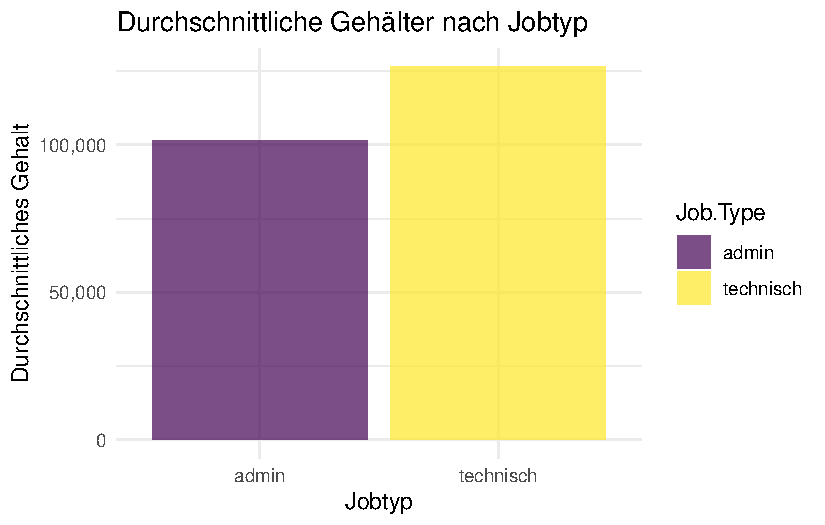
\includegraphics{main_doc_files/figure-pdf/unnamed-chunk-83-1.pdf}

}

\end{figure}

In dem Balkendiagramm ist deutlich zu erkennen, dass das
durchscnittliche Gehalt bei den technischen Jobs höher ist.

Anschließend werden die Werte der durchschnittlichen Gehälter auch
nochmal separat ohne Grafik ausgegeben:

\begin{Shaded}
\begin{Highlighting}[]
\NormalTok{technische\_jobs }\OtherTok{\textless{}{-}} \FunctionTok{subset}\NormalTok{(filtered\_data, job\_type }\SpecialCharTok{==} \DecValTok{0}\NormalTok{)}
\NormalTok{admin\_jobs }\OtherTok{\textless{}{-}} \FunctionTok{subset}\NormalTok{(filtered\_data, job\_type }\SpecialCharTok{==} \DecValTok{1}\NormalTok{)}

\NormalTok{average\_salaries\_technical }\OtherTok{\textless{}{-}} \FunctionTok{mean}\NormalTok{(technische\_jobs}\SpecialCharTok{$}\NormalTok{Salary, }\AttributeTok{na.rm =} \ConstantTok{TRUE}\NormalTok{)}

\NormalTok{average\_salaries\_admin }\OtherTok{\textless{}{-}} \FunctionTok{mean}\NormalTok{(admin\_jobs}\SpecialCharTok{$}\NormalTok{Salary, }\AttributeTok{na.rm =} \ConstantTok{TRUE}\NormalTok{)}

\FunctionTok{cat}\NormalTok{(}\StringTok{"Durchschnittliches Gehalt für technische Jobs:"}\NormalTok{, average\_salaries\_technical, }\StringTok{"}\SpecialCharTok{\textbackslash{}n}\StringTok{"}\NormalTok{)}
\end{Highlighting}
\end{Shaded}

\begin{verbatim}
Durchschnittliches Gehalt für technische Jobs: 126441.3 
\end{verbatim}

\begin{Shaded}
\begin{Highlighting}[]
\FunctionTok{cat}\NormalTok{(}\StringTok{"Durchschnittliches Gehalt für administrative Jobs:"}\NormalTok{, average\_salaries\_admin, }\StringTok{"}\SpecialCharTok{\textbackslash{}n}\StringTok{"}\NormalTok{)}
\end{Highlighting}
\end{Shaded}

\begin{verbatim}
Durchschnittliches Gehalt für administrative Jobs: 101595.3 
\end{verbatim}

Auch hier ist zu erkennen, dass das durchschnittliche Gehalt bei
technischen Jobs um rund 20.000 GE höher ist.

\hypertarget{je-land}{%
\subsubsection{6.4.3.: Je Land}\label{je-land}}

Nun wird eine Übersicht der durchschnittlichen Gehälter nach der
Sortierung der Jobs, je Land erstellt.

\begin{Shaded}
\begin{Highlighting}[]
\NormalTok{summary\_data }\OtherTok{\textless{}{-}} \FunctionTok{aggregate}\NormalTok{(Salary }\SpecialCharTok{\textasciitilde{}}\NormalTok{ Education.Level }\SpecialCharTok{+}\NormalTok{ Country, }\AttributeTok{data =}\NormalTok{ filtered\_data, }\AttributeTok{FUN =}\NormalTok{ median)}

\FunctionTok{ggplot}\NormalTok{(summary\_data, }\FunctionTok{aes}\NormalTok{(}\AttributeTok{x =}\NormalTok{ Education.Level, }\AttributeTok{y =}\NormalTok{ Salary, }\AttributeTok{fill =}\NormalTok{ Country)) }\SpecialCharTok{+}
  \FunctionTok{geom\_bar}\NormalTok{(}\AttributeTok{stat =} \StringTok{"identity"}\NormalTok{, }\AttributeTok{position =} \StringTok{"dodge"}\NormalTok{) }\SpecialCharTok{+}
  \FunctionTok{scale\_fill\_viridis}\NormalTok{(}\AttributeTok{discrete =} \ConstantTok{TRUE}\NormalTok{) }\SpecialCharTok{+}
  \FunctionTok{labs}\NormalTok{(}\AttributeTok{title =} \StringTok{"Median Gehalt nach Bildungslevel und Land"}\NormalTok{, }
       \AttributeTok{x =} \StringTok{"Bildungslevel"}\NormalTok{,}
       \AttributeTok{y =} \StringTok{"Median Gehalt"}\NormalTok{,}
       \AttributeTok{fill =} \StringTok{"Land"}\NormalTok{) }\SpecialCharTok{+}
  \FunctionTok{theme\_minimal}\NormalTok{()}
\end{Highlighting}
\end{Shaded}

\begin{figure}[H]

{\centering 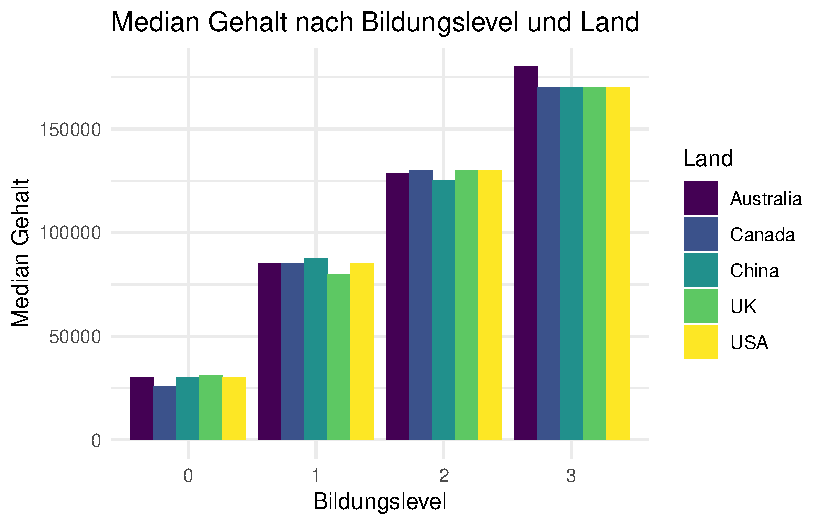
\includegraphics{main_doc_files/figure-pdf/unnamed-chunk-85-1.pdf}

}

\end{figure}

Die These ergibt sich als korrekt und das obwohl in den Admin Jobs auch
in seltenen Fällen Manager vertreten sind.

Es lässt sich zudem beobachten, dass Doktoren in Australien ein höheres
Gehalt verdienen als in anderen Ländern.

\hypertarget{data-scientist-verdienen-aufgrund-der-hohen-nachfrage-der-berufsgruppe-im-schnitt-mehr-als-andere-jobgruppen-bei-gleichbleibender-erfahrung-und-abschlussniveau.}{%
\subsection{6.5 Data Scientist verdienen aufgrund der hohen Nachfrage
der Berufsgruppe im Schnitt mehr als andere Jobgruppen bei
gleichbleibender Erfahrung und
Abschlussniveau.}\label{data-scientist-verdienen-aufgrund-der-hohen-nachfrage-der-berufsgruppe-im-schnitt-mehr-als-andere-jobgruppen-bei-gleichbleibender-erfahrung-und-abschlussniveau.}}

\hypertarget{begruxfcndung}{%
\subsubsection{6.5.1.: Begründung}\label{begruxfcndung}}

Der Beruf des Data Scientist ist laut dem Harvard Business Review der
``Sexiest Job of the 21st Century''.

Siehe Link:

*\url{https://hbr.org/2012/10/data-scientist-the-sexiest-job-of-the-21st-century}

Nach Anbetracht dieser Aussage, stellt sich die Frage, ob gerade das
Gehalt von Data Scientists, zu dieser Aussage führt.

\hypertarget{datenaufbereitung}{%
\subsubsection{6.5.2.: Datenaufbereitung}\label{datenaufbereitung}}

Um die These beantworten zu können, müssen als erstes ein paar
Anpassungen an dem Datensatz vorgenommen werden.

Zunächst wird eine Einengung nach Jobs, nach den Stichworten Data,
Software, Developer und Egineer durchgeführt. Anschließend werden alle
Manager und Direktoren rausgefiltert.

\begin{Shaded}
\begin{Highlighting}[]
\NormalTok{filtered\_data3 }\OtherTok{\textless{}{-}}\NormalTok{ filtered\_data }\SpecialCharTok{\%\textgreater{}\%}
  \FunctionTok{filter}\NormalTok{(}\FunctionTok{grepl}\NormalTok{(}\StringTok{"Data|Software|Developer|Engineer"}\NormalTok{, Job.Title))}

\NormalTok{job\_title\_count }\OtherTok{\textless{}{-}} \FunctionTok{table}\NormalTok{(filtered\_data3}\SpecialCharTok{$}\NormalTok{Job.Title)}
\NormalTok{job\_title\_df }\OtherTok{\textless{}{-}} \FunctionTok{data.frame}\NormalTok{(}\AttributeTok{Job\_Title =} \FunctionTok{names}\NormalTok{(job\_title\_count), }\AttributeTok{Frequency =} \FunctionTok{as.numeric}\NormalTok{(job\_title\_count))}

\NormalTok{job\_title\_df}
\end{Highlighting}
\end{Shaded}

\begin{verbatim}
                   Job_Title Frequency
1         Back end Developer       242
2               Data Analyst       391
3             Data Scientist       515
4   Director of Data Science        57
5        Front end Developer       239
6        Front End Developer        31
7        Full Stack Engineer       304
8           Project Engineer       317
9         Software Developer       186
10         Software Engineer       809
11 Software Engineer Manager       376
12             Web Developer       129
\end{verbatim}

\begin{Shaded}
\begin{Highlighting}[]
\NormalTok{filtered\_data3 }\OtherTok{\textless{}{-}}\NormalTok{ filtered\_data3 }\SpecialCharTok{\%\textgreater{}\%}
  \FunctionTok{filter}\NormalTok{(}\SpecialCharTok{!}\FunctionTok{grepl}\NormalTok{(}\StringTok{"Director|Manager"}\NormalTok{, Job.Title))}

\NormalTok{job\_title\_count }\OtherTok{\textless{}{-}} \FunctionTok{table}\NormalTok{(filtered\_data3}\SpecialCharTok{$}\NormalTok{Job.Title)}
\NormalTok{job\_title\_df }\OtherTok{\textless{}{-}} \FunctionTok{data.frame}\NormalTok{(}\AttributeTok{Job\_Title =} \FunctionTok{names}\NormalTok{(job\_title\_count), }\AttributeTok{Frequency =} \FunctionTok{as.numeric}\NormalTok{(job\_title\_count))}

\NormalTok{job\_title\_df}
\end{Highlighting}
\end{Shaded}

\begin{verbatim}
             Job_Title Frequency
1   Back end Developer       242
2         Data Analyst       391
3       Data Scientist       515
4  Front end Developer       239
5  Front End Developer        31
6  Full Stack Engineer       304
7     Project Engineer       317
8   Software Developer       186
9    Software Engineer       809
10       Web Developer       129
\end{verbatim}

Anschließend wird, um die Leserlichkeit zu verbessern, eine Aufteilung
der Jobs durchgeführt. Hierzu werden die Jobs in eine neue Spalte
``data\_job'' aufgeteilt.

\begin{Shaded}
\begin{Highlighting}[]
\NormalTok{filtered\_data3 }\OtherTok{\textless{}{-}}\NormalTok{ filtered\_data3 }\SpecialCharTok{\%\textgreater{}\%}
  \FunctionTok{mutate}\NormalTok{(}\AttributeTok{data\_job =} \FunctionTok{ifelse}\NormalTok{(}\FunctionTok{grepl}\NormalTok{(}\StringTok{"Data"}\NormalTok{, Job.Title), }\DecValTok{1}\NormalTok{, }\DecValTok{0}\NormalTok{))}
\end{Highlighting}
\end{Shaded}

\begin{Shaded}
\begin{Highlighting}[]
\NormalTok{count\_0 }\OtherTok{\textless{}{-}} \FunctionTok{sum}\NormalTok{(filtered\_data3}\SpecialCharTok{$}\NormalTok{data\_job }\SpecialCharTok{==} \DecValTok{0}\NormalTok{, }\AttributeTok{na.rm =} \ConstantTok{TRUE}\NormalTok{)}
\NormalTok{count\_1 }\OtherTok{\textless{}{-}} \FunctionTok{sum}\NormalTok{(filtered\_data3}\SpecialCharTok{$}\NormalTok{data\_job }\SpecialCharTok{==} \DecValTok{1}\NormalTok{, }\AttributeTok{na.rm =} \ConstantTok{TRUE}\NormalTok{)}

\FunctionTok{cat}\NormalTok{(}\StringTok{"Anzahl der Zeilen mit dem Wert 0 bei data\_job (Data Scientists \& Engineers):"}\NormalTok{, count\_0, }\StringTok{"}\SpecialCharTok{\textbackslash{}n}\StringTok{"}\NormalTok{)}
\end{Highlighting}
\end{Shaded}

\begin{verbatim}
Anzahl der Zeilen mit dem Wert 0 bei data_job (Data Scientists & Engineers): 2257 
\end{verbatim}

\begin{Shaded}
\begin{Highlighting}[]
\FunctionTok{cat}\NormalTok{(}\StringTok{"Anzahl der Zeilen mit dem Wert 1 bei data\_job (Software Engineers \& Co):"}\NormalTok{, count\_1, }\StringTok{"}\SpecialCharTok{\textbackslash{}n}\StringTok{"}\NormalTok{)}
\end{Highlighting}
\end{Shaded}

\begin{verbatim}
Anzahl der Zeilen mit dem Wert 1 bei data_job (Software Engineers & Co): 906 
\end{verbatim}

\hypertarget{balkendiagramm}{%
\subsubsection{6.5.3.: Balkendiagramm}\label{balkendiagramm}}

Um die Übersicht zu verbessern, wird die Berufserfahrung in Quantile
eingeteilt. Die Bildungsniveaus hingegen wurden bereits im Vorfeld in
vier Werte eingeteilt.

Als erstes werden die Quantile der Berufserfahrung berechnet und
anschließend ein Balkendiagramm für den Datensatz ``data\_job''
erstellt, um das Gehalt zu vergleichen.

\begin{Shaded}
\begin{Highlighting}[]
\NormalTok{filtered\_data4 }\OtherTok{\textless{}{-}}\NormalTok{ filtered\_data3 }\SpecialCharTok{\%\textgreater{}\%}
  \FunctionTok{mutate}\NormalTok{(}\AttributeTok{Experience\_Quartile =} \FunctionTok{ntile}\NormalTok{(Years.Of.Experience, }\DecValTok{4}\NormalTok{))}

\FunctionTok{ggplot}\NormalTok{(filtered\_data4, }\FunctionTok{aes}\NormalTok{(}\AttributeTok{x =} \FunctionTok{factor}\NormalTok{(data\_job), }\AttributeTok{y =}\NormalTok{ Salary)) }\SpecialCharTok{+}
  \FunctionTok{stat\_summary}\NormalTok{(}\AttributeTok{fun =} \StringTok{"mean"}\NormalTok{, }\AttributeTok{geom =} \StringTok{"bar"}\NormalTok{, }\AttributeTok{position =} \StringTok{"dodge"}\NormalTok{, }\AttributeTok{fill =} \FunctionTok{viridis}\NormalTok{(}\DecValTok{2}\NormalTok{)[}\DecValTok{1}\NormalTok{]) }\SpecialCharTok{+}
  \FunctionTok{labs}\NormalTok{(}\AttributeTok{title =} \StringTok{"Gehalt nach Data Job"}\NormalTok{,}
       \AttributeTok{x =} \StringTok{"Data Job"}\NormalTok{,}
       \AttributeTok{y =} \StringTok{"Gehalt (Mittelwert)"}\NormalTok{)}
\end{Highlighting}
\end{Shaded}

\begin{figure}[H]

{\centering 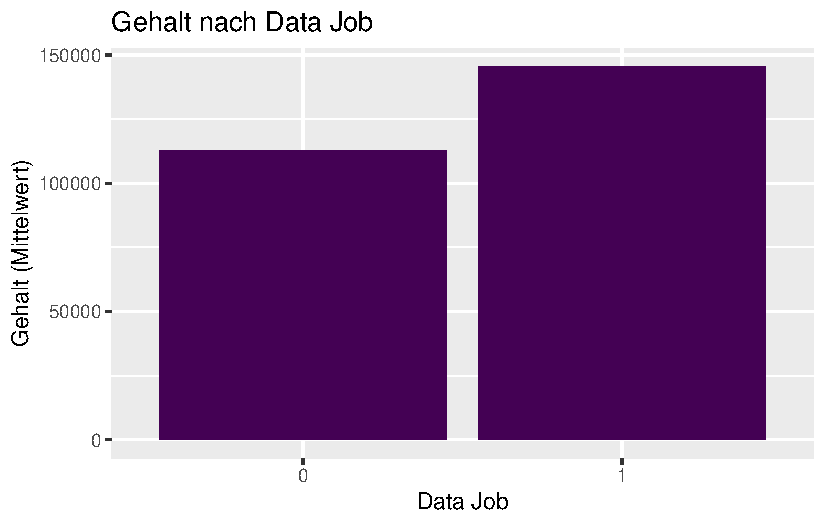
\includegraphics{main_doc_files/figure-pdf/unnamed-chunk-90-1.pdf}

}

\end{figure}

\begin{Shaded}
\begin{Highlighting}[]
\FunctionTok{ggplot}\NormalTok{(filtered\_data4, }\FunctionTok{aes}\NormalTok{(}\AttributeTok{y =}\NormalTok{ Salary, }\AttributeTok{x =} \FunctionTok{factor}\NormalTok{(Experience\_Quartile))) }\SpecialCharTok{+}
  \FunctionTok{geom\_bar}\NormalTok{(}\AttributeTok{stat =} \StringTok{"identity"}\NormalTok{, }\AttributeTok{position =} \StringTok{"dodge"}\NormalTok{, }\FunctionTok{aes}\NormalTok{(}\AttributeTok{fill =} \FunctionTok{factor}\NormalTok{(data\_job))) }\SpecialCharTok{+}
  \FunctionTok{labs}\NormalTok{(}\AttributeTok{title =} \StringTok{"Quartile der Berufserfahrung nach Gehalt und Jobtyp"}\NormalTok{,}
       \AttributeTok{x =} \StringTok{"Quartile der Berufserfahrung"}\NormalTok{,}
       \AttributeTok{y =} \StringTok{"Gehalt"}\NormalTok{) }\SpecialCharTok{+}
  \FunctionTok{theme\_minimal}\NormalTok{() }\SpecialCharTok{+}
  \FunctionTok{scale\_fill\_viridis}\NormalTok{(}\AttributeTok{discrete =} \ConstantTok{TRUE}\NormalTok{)}
\end{Highlighting}
\end{Shaded}

\begin{figure}[H]

{\centering 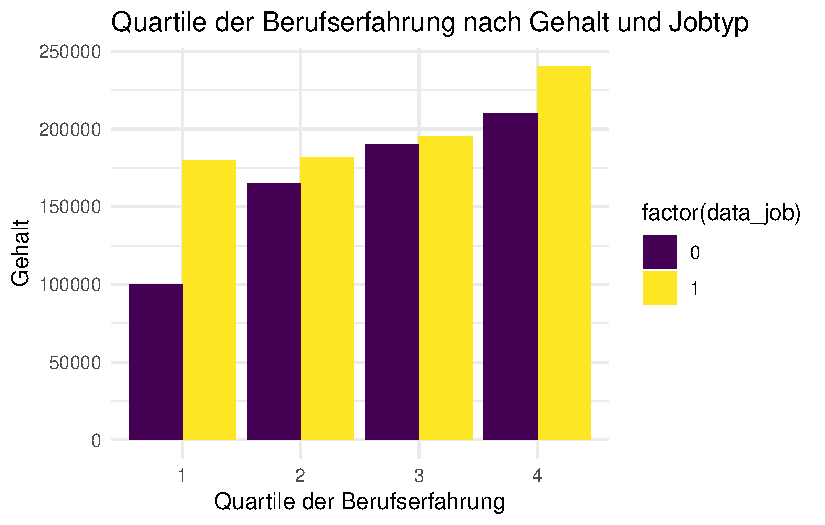
\includegraphics{main_doc_files/figure-pdf/unnamed-chunk-91-1.pdf}

}

\end{figure}

Zum Verständnis hier noch einmal die Codes des Bidlungsniveaus

0 = High School Abschluss

1 = Bachelor

2 = Master

3 = Doctor

\begin{Shaded}
\begin{Highlighting}[]
\FunctionTok{ggplot}\NormalTok{(filtered\_data4, }\FunctionTok{aes}\NormalTok{(}\AttributeTok{y =}\NormalTok{ Salary, }\AttributeTok{x =} \FunctionTok{factor}\NormalTok{(Education.Level))) }\SpecialCharTok{+}
  \FunctionTok{geom\_bar}\NormalTok{(}\AttributeTok{stat =} \StringTok{"identity"}\NormalTok{, }\AttributeTok{position =} \StringTok{"dodge"}\NormalTok{, }\FunctionTok{aes}\NormalTok{(}\AttributeTok{fill =} \FunctionTok{factor}\NormalTok{(data\_job))) }\SpecialCharTok{+}
  \FunctionTok{scale\_fill\_viridis}\NormalTok{(}\AttributeTok{discrete =} \ConstantTok{TRUE}\NormalTok{) }\SpecialCharTok{+}
  \FunctionTok{labs}\NormalTok{(}\AttributeTok{title =} \StringTok{"Quartile des Bildungsniveaus nach Gehalt und Jobtyp"}\NormalTok{,}
       \AttributeTok{x =} \StringTok{"Quartile des Bildungsniveaus"}\NormalTok{,}
       \AttributeTok{y =} \StringTok{"Gehalt"}\NormalTok{) }\SpecialCharTok{+}
  \FunctionTok{theme\_minimal}\NormalTok{()}
\end{Highlighting}
\end{Shaded}

\begin{figure}[H]

{\centering 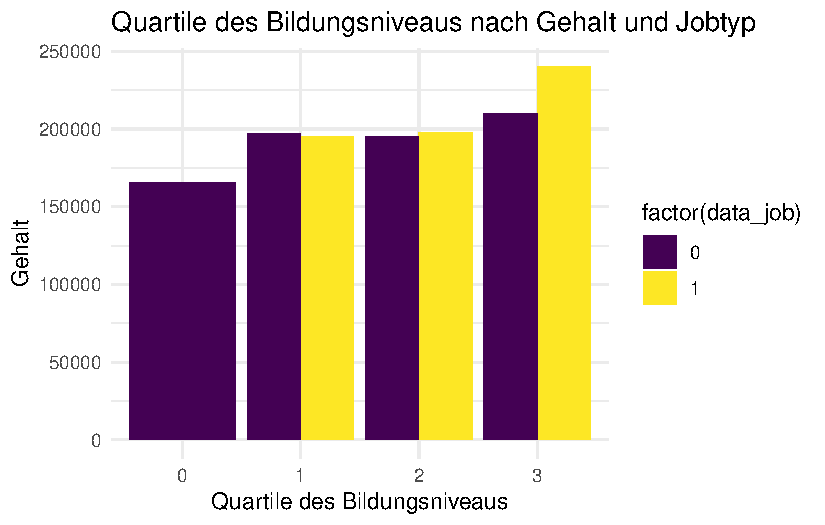
\includegraphics{main_doc_files/figure-pdf/unnamed-chunk-92-1.pdf}

}

\end{figure}

Hier ist zu erkennen, dass Data Scientists mehr als Arbeitnehmer aus der
Software Enginnering \% Co Gruppe. Es muss jedoch beachtet werden, dass
die ``data- Gruppe'' mindestens einen Bachelor besitzt und erst nach
einem Master mehr verdient, als ihr Counterpart. Im Bezug auf die
Berufserfahrung lässt sich feststellen, dass es in jedem Quantil einen
höheres Gehaltsniveau bei der ``data-Gruppe'' gibt.

Trotzdem lässt sich sagen, dass die These korrekt ist.

\hypertarget{die-gehuxe4lter-sind-in-luxe4ndern-mit-einem-huxf6heren-bip-pro-kopf-huxf6her}{%
\subsection{6.6 Die Gehälter sind in Ländern mit einem höheren BIP pro
Kopf
höher}\label{die-gehuxe4lter-sind-in-luxe4ndern-mit-einem-huxf6heren-bip-pro-kopf-huxf6her}}

Zum Verständnis sind hier einmal die BIP's pro Kopf aus externen Quellen
aufgelistet, da diese nicht im Datensatz vertreten sind:

Australien 64.813,85 US-Dollar Quelle:
\href{https://de.statista.com/statistik/daten/studie/14425/umfrage/bruttoinlandsprodukt-pro-kopf-in-australien/\#:~:text=Im\%20Jahr\%202022\%20hat\%20das\%20Bruttoinlandsprodukt\%20pro\%20Kopf,Kopf\%20in\%20Australien\%20auf\%20rund\%2063.487\%2C05\%20US-Dollar\%20prognostiziert.}{Australien
- BIP pro Kopf bis 2028 \textbar{} Statista}

Canada 53.246,98 US-Dollar Quelle:
\href{https://de.statista.com/statistik/daten/studie/14428/umfrage/bruttoinlandsprodukt-pro-kopf-in-kanada/\#:~:text=Im\%20Jahr\%202022\%20hat\%20das\%20Bruttoinlandsprodukt\%20pro\%20Kopf,bis\%202022\%20und\%20Prognosen\%20bis\%20zum\%20Jahr\%202028.}{Kanada
- BIP pro Kopf bis 2028 \textbar{} Statista}

China 12.541,40 US-Dollar Quelle:
\href{https://de.statista.com/statistik/daten/studie/19407/umfrage/bruttoinlandsprodukt-pro-kopf-in-china/\#:~:text=Im\%20Jahr\%202022\%20hat\%20das\%20Bruttoinlandsprodukt\%20pro\%20Kopf,bis\%202022\%20und\%20Prognosen\%20bis\%20zum\%20Jahr\%202028.}{China
- BIP pro Kopf bis 2028 \textbar{} Statista}

UK 48.912,78 US-Dollar Quelle:
\href{https://de.statista.com/statistik/daten/studie/14453/umfrage/bruttoinlandsprodukt-pro-kopf-in-grossbritannien/\#:~:text=F\%C3\%BCr\%20das\%20Jahr\%202023\%20wird\%20das\%20Bruttoinlandsprodukt\%20pro,bis\%202020\%20und\%20Prognosen\%20bis\%20zum\%20Jahr\%202028.}{Großbritannien
- BIP pro Kopf bis 2028 \textbar{} Statista}

USA 76.343 US-Dollar Quelle:
\href{https://de.statista.com/statistik/daten/studie/14454/umfrage/bruttoinlandsprodukt-pro-kopf-in-den-usa/}{USA
- BIP pro Kopf bis 2028 \textbar{} Statista}

\hypertarget{aufbereitung}{%
\subsubsection{6.6.1.: Aufbereitung}\label{aufbereitung}}

Vorab muss ein wenig Vorarbeit geleistet werden.

Zunächst werden die BIP-Werte den entsprechend Ländern zugewiesen.

\begin{Shaded}
\begin{Highlighting}[]
\NormalTok{filtered\_data}\SpecialCharTok{$}\NormalTok{BIP\_Per\_Person }\OtherTok{\textless{}{-}} \ConstantTok{NA}

\NormalTok{filtered\_data}\SpecialCharTok{$}\NormalTok{BIP\_Per\_Person[filtered\_data}\SpecialCharTok{$}\NormalTok{Country }\SpecialCharTok{==} \StringTok{"Australia"}\NormalTok{] }\OtherTok{\textless{}{-}} \FloatTok{64813.85}
\NormalTok{filtered\_data}\SpecialCharTok{$}\NormalTok{BIP\_Per\_Person[filtered\_data}\SpecialCharTok{$}\NormalTok{Country }\SpecialCharTok{==} \StringTok{"Canada"}\NormalTok{] }\OtherTok{\textless{}{-}} \FloatTok{53246.98}
\NormalTok{filtered\_data}\SpecialCharTok{$}\NormalTok{BIP\_Per\_Person[filtered\_data}\SpecialCharTok{$}\NormalTok{Country }\SpecialCharTok{==} \StringTok{"China"}\NormalTok{] }\OtherTok{\textless{}{-}} \FloatTok{12541.40}
\NormalTok{filtered\_data}\SpecialCharTok{$}\NormalTok{BIP\_Per\_Person[filtered\_data}\SpecialCharTok{$}\NormalTok{Country }\SpecialCharTok{==} \StringTok{"UK"}\NormalTok{] }\OtherTok{\textless{}{-}} \FloatTok{48912.78}
\NormalTok{filtered\_data}\SpecialCharTok{$}\NormalTok{BIP\_Per\_Person[filtered\_data}\SpecialCharTok{$}\NormalTok{Country }\SpecialCharTok{==} \StringTok{"USA"}\NormalTok{] }\OtherTok{\textless{}{-}} \FloatTok{76343.00}
\end{Highlighting}
\end{Shaded}

\begin{Shaded}
\begin{Highlighting}[]
\FunctionTok{head}\NormalTok{(filtered\_data3)}
\end{Highlighting}
\end{Shaded}

\begin{verbatim}
# A tibble: 6 x 15
  Job.Title    job_count   Age Gender Education.Level Years.Of.Experience Salary
  <chr>            <int> <dbl> <chr>  <fct>                         <dbl>  <dbl>
1 Back end De~       242    33 Female 2                                 5 110000
2 Back end De~       242    32 Male   1                                 4  95000
3 Back end De~       242    26 Female 2                                 3  90000
4 Back end De~       242    26 Female 2                                 2  70000
5 Back end De~       242    24 Female 1                                 1  60000
6 Back end De~       242    26 Female 2                                 3  90000
# i 8 more variables: Country <chr>, Race <chr>, Senior <dbl>, SalaryKat <fct>,
#   ID <int>, job_type <dbl>, Expat <dbl>, data_job <dbl>
\end{verbatim}

\hypertarget{visualisierung-und-berechnung}{%
\subsubsection{6.6.2.: Visualisierung und
Berechnung}\label{visualisierung-und-berechnung}}

Mithilfe von Streudiagrammen und Berechnungen wird nun versucht die
These zu widerlegen oder als richtig markieren zu können.

\begin{Shaded}
\begin{Highlighting}[]
\FunctionTok{ggplot}\NormalTok{(filtered\_data, }\FunctionTok{aes}\NormalTok{(}\AttributeTok{x =}\NormalTok{ BIP\_Per\_Person, }\AttributeTok{y =}\NormalTok{ Salary, }\AttributeTok{color =}\NormalTok{ Country)) }\SpecialCharTok{+}
  \FunctionTok{geom\_point}\NormalTok{() }\SpecialCharTok{+}
  \FunctionTok{stat\_summary}\NormalTok{(}\AttributeTok{fun =}\NormalTok{ mean, }\AttributeTok{geom =} \StringTok{"point"}\NormalTok{, }\AttributeTok{shape =} \DecValTok{23}\NormalTok{, }\AttributeTok{size =} \DecValTok{3}\NormalTok{, }\AttributeTok{fill =} \StringTok{"black"}\NormalTok{) }\SpecialCharTok{+}
  \FunctionTok{labs}\NormalTok{(}\AttributeTok{title =} \StringTok{"Vergleich von Gehalt und BIP pro Person nach Ländern"}\NormalTok{,}
       \AttributeTok{x =} \StringTok{"BIP pro Person"}\NormalTok{,}
       \AttributeTok{y =} \StringTok{"Gehalt"}\NormalTok{,}
       \AttributeTok{color =} \StringTok{"Land"}\NormalTok{) }\SpecialCharTok{+}
  \FunctionTok{scale\_color\_viridis}\NormalTok{(}\AttributeTok{discrete =} \ConstantTok{TRUE}\NormalTok{)}
\end{Highlighting}
\end{Shaded}

\begin{figure}[H]

{\centering 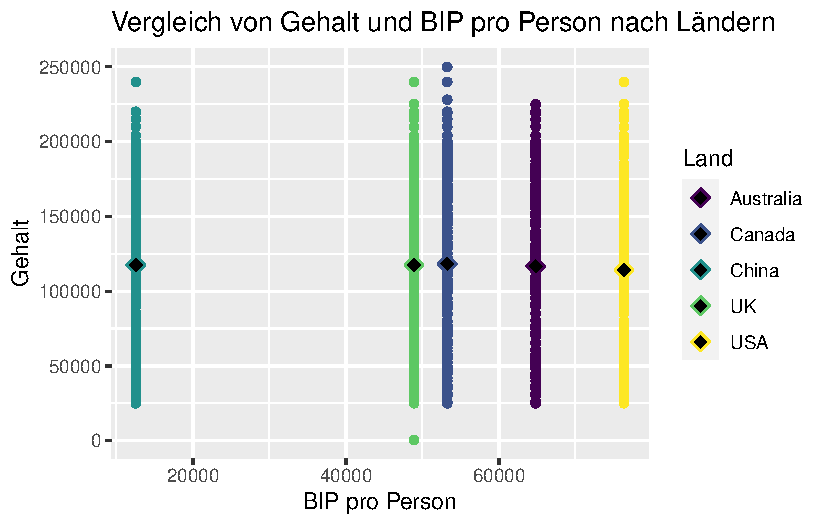
\includegraphics{main_doc_files/figure-pdf/unnamed-chunk-95-1.pdf}

}

\end{figure}

Mithilfe dieses Streudiagramm ist viel zu erkennen. Deswegen werden
weitere Berechnungen angestellt.

Zunächst werden die Mittelwerte nach Land berechnet und anschließend die
Mittelwerte nach Land in Bezug auf das BIP.

\begin{Shaded}
\begin{Highlighting}[]
\NormalTok{mean\_salaries\_by\_country }\OtherTok{\textless{}{-}}\NormalTok{ filtered\_data3 }\SpecialCharTok{\%\textgreater{}\%}
  \FunctionTok{group\_by}\NormalTok{(Country) }\SpecialCharTok{\%\textgreater{}\%}
  \FunctionTok{summarise}\NormalTok{(}\AttributeTok{mean\_salary =} \FunctionTok{mean}\NormalTok{(Salary, }\AttributeTok{na.rm =} \ConstantTok{TRUE}\NormalTok{))}

\NormalTok{mean\_salaries\_by\_country}
\end{Highlighting}
\end{Shaded}

\begin{verbatim}
# A tibble: 5 x 2
  Country   mean_salary
  <chr>           <dbl>
1 Australia     121610.
2 Canada        125466.
3 China         120395.
4 UK            123564.
5 USA           119265.
\end{verbatim}

\begin{Shaded}
\begin{Highlighting}[]
\NormalTok{mean\_salaries\_by\_country }\OtherTok{\textless{}{-}}\NormalTok{ filtered\_data }\SpecialCharTok{\%\textgreater{}\%}
  \FunctionTok{group\_by}\NormalTok{(Country) }\SpecialCharTok{\%\textgreater{}\%}
  \FunctionTok{summarise}\NormalTok{(}\AttributeTok{mean\_salary =} \FunctionTok{mean}\NormalTok{(Salary, }\AttributeTok{na.rm =} \ConstantTok{TRUE}\NormalTok{),}
            \AttributeTok{BIP\_Per\_Person =} \FunctionTok{first}\NormalTok{(BIP\_Per\_Person))  }
\NormalTok{mean\_salaries\_by\_country}
\end{Highlighting}
\end{Shaded}

\begin{verbatim}
# A tibble: 5 x 3
  Country   mean_salary BIP_Per_Person
  <chr>           <dbl>          <dbl>
1 Australia     116704.         64814.
2 Canada        118200.         53247.
3 China         117480.         12541.
4 UK            117412.         48913.
5 USA           114209.         76343 
\end{verbatim}

Außerdem wird noch die Korrelation zwischen der Salary und dem BIP
Berechnet.

\begin{Shaded}
\begin{Highlighting}[]
\FunctionTok{cor}\NormalTok{(filtered\_data}\SpecialCharTok{$}\NormalTok{Salary, filtered\_data}\SpecialCharTok{$}\NormalTok{BIP\_Per\_Person, }\AttributeTok{use =} \StringTok{"complete.obs"}\NormalTok{)}
\end{Highlighting}
\end{Shaded}

\begin{verbatim}
[1] -0.01632912
\end{verbatim}

Es geht hervor, dass es keine große Korrelation ziwschen dem Gehalt und
dem BIP gibt.

Nun wird das Ganze noch ohne China durchgeführt:

Zunächst wird ein Datensatz ohne China erstellt und anschließend wird
die Korrelation erneut berechnet. Zudem wird die Anzahl der Datensätze
mit dem land ``China'' in dem neuen Datensatz festgehalten.

\begin{Shaded}
\begin{Highlighting}[]
\NormalTok{filtered\_data\_no\_china }\OtherTok{\textless{}{-}}\NormalTok{ filtered\_data }\SpecialCharTok{\%\textgreater{}\%} \FunctionTok{filter}\NormalTok{(Country }\SpecialCharTok{!=} \StringTok{"China"}\NormalTok{)}
\end{Highlighting}
\end{Shaded}

\begin{Shaded}
\begin{Highlighting}[]
\FunctionTok{cor}\NormalTok{(filtered\_data\_no\_china}\SpecialCharTok{$}\NormalTok{Salary, filtered\_data\_no\_china}\SpecialCharTok{$}\NormalTok{BIP\_Per\_Person, }\AttributeTok{use =} \StringTok{"complete.obs"}\NormalTok{)}
\end{Highlighting}
\end{Shaded}

\begin{verbatim}
[1] -0.02614532
\end{verbatim}

\begin{Shaded}
\begin{Highlighting}[]
\NormalTok{count\_china }\OtherTok{\textless{}{-}}\NormalTok{ filtered\_data\_no\_china }\SpecialCharTok{\%\textgreater{}\%} \FunctionTok{filter}\NormalTok{(Country }\SpecialCharTok{==} \StringTok{"China"}\NormalTok{) }\SpecialCharTok{\%\textgreater{}\%} \FunctionTok{nrow}\NormalTok{()}
\NormalTok{count\_china}
\end{Highlighting}
\end{Shaded}

\begin{verbatim}
[1] 0
\end{verbatim}

Anhand der Berechnung und des Streudiagramms, lässt sich die These als
nicht korrekt beantworten. Es gibt eine negative Korrelation zwischen
dem Gehalt, welches ein Arbeitnehmer erhält und dem BIP des jeweiligen
Landes. Selbst wenn China aus der Berechnung rausgenommen wird, welches
aufgrund der hohen Einwohnerzahl und diversen Wirtschaft
(Sonderverwaltungszonen und Kommunismus) einen sehr niedrigen BIP hat.

Nun stellt sich die Frage, ob eventuell in dem Datensatz bewusst Jobs
mit hohem Gehalt gewählt wurden. Oder wurden Werte von spezifischen
Firmen, die international tätig sind und gut bezahlen, genommen?

Siehe folgende Links:

*\url{https://de.wikipedia.org/wiki/Politisches_System_der_Volksrepublik_China}

*\url{https://de.wikipedia.org/wiki/Sonderverwaltungszone}

\hypertarget{regressionen}{%
\section{7. Regressionen}\label{regressionen}}

In dem folgenden Absatz werden die Regressionen durchgeführt.

\hypertarget{einfache-lineare-regression-gehalt-und-arbeitserfahrung}{%
\subsection{7.1.: Einfache Lineare Regression Gehalt und
Arbeitserfahrung}\label{einfache-lineare-regression-gehalt-und-arbeitserfahrung}}

Zu Beginn wird eine einfache lineare Regression mit dem Gehalt und der
Arbeitserfahrung durchgeführt

Die Korrelation von Arbeitserfahrung und Gehalt liegt bei 0.81, weshalb
wir uns entscheiden haben diese als Regression zu verwenden. Des
weiteren nutzen wir zusätzlich das Alter und das Bildungsniveau.

Die Korrelation zwischen der Arbeitserfahrung und Gehalt liegt bei 0.81.
Deshalb wurde entschieden diese als Regression zu verwenden. Des
Weiteren wird auch das Alter, so wie das Bildungsniveau verwendet.

\hypertarget{korrelationsmatrix}{%
\subsubsection{7.1.1.: Korrelationsmatrix}\label{korrelationsmatrix}}

Zunächst wird ein Streudiagramm über die Beziehung zwischen dem Gehalt
und der Berufserfahrung erstellt. Außerdem wird eine lineare
Regressionsgerade eingefügt, um den Trend besser analysieren zu können.

\begin{Shaded}
\begin{Highlighting}[]
\NormalTok{filtered\_data }\SpecialCharTok{\%\textgreater{}\%}
  \FunctionTok{ggplot}\NormalTok{() }\SpecialCharTok{+}
  \FunctionTok{aes}\NormalTok{(}\AttributeTok{y =}\NormalTok{ Salary, }\AttributeTok{x =}\NormalTok{ Years.Of.Experience) }\SpecialCharTok{+}
  \FunctionTok{geom\_point}\NormalTok{(}\FunctionTok{aes}\NormalTok{(}\AttributeTok{color =}\NormalTok{ Salary), }\AttributeTok{alpha =} \FloatTok{0.8}\NormalTok{) }\SpecialCharTok{+}
  \FunctionTok{geom\_smooth}\NormalTok{(}\AttributeTok{method =}\NormalTok{ lm, }\AttributeTok{color =} \StringTok{"orange"}\NormalTok{) }\SpecialCharTok{+}
  \FunctionTok{scale\_color\_viridis}\NormalTok{(}\AttributeTok{option =} \StringTok{"D"}\NormalTok{) }\SpecialCharTok{+}
  \FunctionTok{scale\_y\_continuous}\NormalTok{(}\AttributeTok{labels =}\NormalTok{ scales}\SpecialCharTok{::}\NormalTok{comma)}
\end{Highlighting}
\end{Shaded}

\begin{verbatim}
`geom_smooth()` using formula = 'y ~ x'
\end{verbatim}

\begin{figure}[H]

{\centering 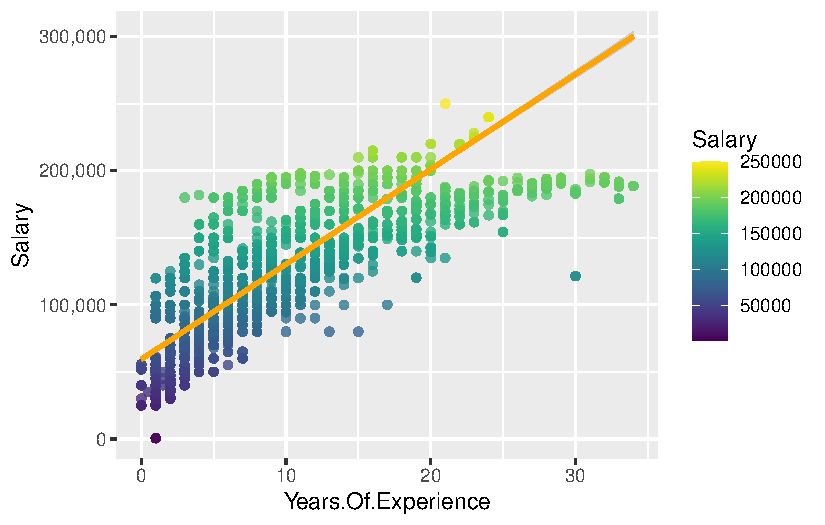
\includegraphics{main_doc_files/figure-pdf/unnamed-chunk-102-1.pdf}

}

\end{figure}

Anhand dieser Grafik kann gesagt werden, dass der Trend deutlich nach
oben geht, je mehr Berufserfahrung eine Person hat.

\hypertarget{datenaufbereitung-1}{%
\subsubsection{7.1.2.: Datenaufbereitung}\label{datenaufbereitung-1}}

Um mit der Regressionsanalyse fortzufahren, müssen noch Änderungen am
Datensatz durchgeführt werden.

Zunächst müssen alle Werte, die nicht für die Regression relevant sind,
entfernt werden. Deswegen werden nur ``Salary'' und ``Years of
Experience'' behalten.

\begin{Shaded}
\begin{Highlighting}[]
\NormalTok{filtered\_data5 }\OtherTok{\textless{}{-}}\NormalTok{ filtered\_data }\SpecialCharTok{\%\textgreater{}\%}
  \FunctionTok{select}\NormalTok{(Salary, Years.Of.Experience)}
\end{Highlighting}
\end{Shaded}

\hypertarget{z-skalierung}{%
\paragraph{7.1.2.1 Z-Skalierung}\label{z-skalierung}}

Zuerst wird eine Z-Skalierung von filtered\_data\_5 durchgeführt.

Die Z-Skalierung ist eine Methode zur Standardisierung von numerischen
Variablen. Bei der Z-Skalierung werden alle numerischen Werte mit
Ausnahme des Vorhersagewerts (Salary) skaliert, um die Auswirkungen von
Ausreißern zu minimieren.

\begin{Shaded}
\begin{Highlighting}[]
\NormalTok{filtered\_data5\_z }\OtherTok{\textless{}{-}}\NormalTok{ filtered\_data5}
\NormalTok{filtered\_data5\_z}\SpecialCharTok{$}\NormalTok{Years.Of.Experience }\OtherTok{\textless{}{-}} \FunctionTok{scale}\NormalTok{(filtered\_data5}\SpecialCharTok{$}\NormalTok{Years.Of.Experience)}
\end{Highlighting}
\end{Shaded}

Ergebnis der Z-Skalierung:

\begin{Shaded}
\begin{Highlighting}[]
\FunctionTok{summary}\NormalTok{(filtered\_data5\_z)}
\end{Highlighting}
\end{Shaded}

\begin{verbatim}
     Salary       Years.Of.Experience.V1
 Min.   :   550   Min.   :-1.350859     
 1st Qu.: 70000   1st Qu.:-0.850649     
 Median :120000   Median :-0.183702     
 Mean   :116787   Mean   : 0.000000     
 3rd Qu.:160000   3rd Qu.: 0.649981     
 Max.   :250000   Max.   : 4.318187     
\end{verbatim}

Überprüfung der Standardabweichung für Arbeitserfahrung

\begin{Shaded}
\begin{Highlighting}[]
\FunctionTok{sd}\NormalTok{(filtered\_data5\_z}\SpecialCharTok{$}\NormalTok{Years.Of.Experience)}
\end{Highlighting}
\end{Shaded}

\begin{verbatim}
[1] 1
\end{verbatim}

Aufteilung in Test- und Trainingsdaten:

\begin{Shaded}
\begin{Highlighting}[]
\FunctionTok{set.seed}\NormalTok{(}\DecValTok{007}\NormalTok{)}

\NormalTok{filtered\_data5\_z }\OtherTok{\textless{}{-}} \FunctionTok{initial\_split}\NormalTok{(filtered\_data5\_z, }\AttributeTok{prop =} \FloatTok{0.8}\NormalTok{, }\AttributeTok{strata =}\NormalTok{ Years.Of.Experience)}

\NormalTok{fd5\_train }\OtherTok{\textless{}{-}} \FunctionTok{training}\NormalTok{(filtered\_data5\_z)}
\NormalTok{fd5\_test }\OtherTok{\textless{}{-}} \FunctionTok{testing}\NormalTok{(filtered\_data5\_z)}
\end{Highlighting}
\end{Shaded}

Dieser Code teilt den Datensatz filtered\_data5\_z in Trainings- und
Testdaten auf, um eine lineare Regression durchzuführen. Die Funktion
set.seed(007) initialisiert den Zufallszahlengenerator mit einer festen
Zahl, um sicherzustellen, dass die Ergebnisse bei jedem Durchlauf
reproduzierbar sind. Die Funktion initial\_split() aus dem Paket rsample
teilt den Datensatz in Trainings- und Testdaten auf. Der Parameter prop
= 0,8 gibt an, dass 80\% der Daten für das Training verwendet werden
sollen, während die restlichen 20\% für das Testen verwendet werden. Der
Parameter strata = Years.Of.Experience sorgt dafür, dass die Daten nach
dem Gehalts-Wert stratifiziert werden, um sicherzustellen, dass die
Trainings- und Testdaten eine ähnliche Verteilung von Gehalts-Werten
aufweisen. Die Funktion training() extrahiert die Trainingsdaten aus dem
aufgeteilten Datensatz, während testing() die Testdaten extrahiert.

\hypertarget{modell-initialisieren}{%
\subsubsection{7.1.3.: Modell
Initialisieren}\label{modell-initialisieren}}

\begin{Shaded}
\begin{Highlighting}[]
\NormalTok{lm\_model }\OtherTok{\textless{}{-}} \FunctionTok{linear\_reg}\NormalTok{() }\SpecialCharTok{|\textgreater{}} \FunctionTok{set\_engine}\NormalTok{(}\StringTok{"lm"}\NormalTok{)}
\end{Highlighting}
\end{Shaded}

Lineare Regression von Salary (basierend auf der Berufserfahrung):

\begin{Shaded}
\begin{Highlighting}[]
\NormalTok{lm\_fit }\OtherTok{\textless{}{-}}\NormalTok{ lm\_model }\SpecialCharTok{|\textgreater{}} \FunctionTok{fit}\NormalTok{(Salary }\SpecialCharTok{\textasciitilde{}}\NormalTok{ Years.Of.Experience, }\AttributeTok{data =}\NormalTok{ fd5\_train)}
\end{Highlighting}
\end{Shaded}

Zusammenfassung vom Ergebnis:

\begin{Shaded}
\begin{Highlighting}[]
\NormalTok{summary }\OtherTok{\textless{}{-}}\NormalTok{ lm\_fit }\SpecialCharTok{|\textgreater{}} \FunctionTok{extract\_fit\_engine}\NormalTok{() }\SpecialCharTok{|\textgreater{}} \FunctionTok{summary}\NormalTok{()}
\NormalTok{summary}
\end{Highlighting}
\end{Shaded}

\begin{verbatim}

Call:
stats::lm(formula = Salary ~ Years.Of.Experience, data = data)

Residuals:
    Min      1Q  Median      3Q     Max 
-149686  -22470   -6278   21338   94530 

Coefficients:
                    Estimate Std. Error t value Pr(>|t|)    
(Intercept)         116445.0      429.6  271.05   <2e-16 ***
Years.Of.Experience  42366.7      428.0   98.98   <2e-16 ***
---
Signif. codes:  0 '***' 0.001 '**' 0.01 '*' 0.05 '.' 0.1 ' ' 1

Residual standard error: 30730 on 5115 degrees of freedom
Multiple R-squared:  0.657, Adjusted R-squared:  0.6569 
F-statistic:  9797 on 1 and 5115 DF,  p-value: < 2.2e-16
\end{verbatim}

Vorhersagen auf Trainings- und Testdatensatz:

Nun werden Vorhersagen für die Tranings-, sowie Testdaten erstellt.
Anschließend werden die tatsächlichen ``Salary''-Werte mit den
Vorhersagen kombiniert. Dies geschieht um zwei seperate Datenrahmen zu
erstellen.

\begin{Shaded}
\begin{Highlighting}[]
\NormalTok{pred\_train }\OtherTok{\textless{}{-}} \FunctionTok{predict}\NormalTok{(lm\_fit, }\AttributeTok{new\_data =}\NormalTok{ fd5\_train) }\SpecialCharTok{|\textgreater{}} \FunctionTok{rename}\NormalTok{(}\StringTok{"pred\_train"} \OtherTok{=} \StringTok{".pred"}\NormalTok{)}
\NormalTok{pred\_test }\OtherTok{\textless{}{-}} \FunctionTok{predict}\NormalTok{(lm\_fit, }\AttributeTok{new\_data =}\NormalTok{ fd5\_test) }\SpecialCharTok{|\textgreater{}}  \FunctionTok{rename}\NormalTok{(}\StringTok{"pred\_test"} \OtherTok{=} \StringTok{".pred"}\NormalTok{)}

\NormalTok{compare\_train }\OtherTok{\textless{}{-}}\NormalTok{ fd5\_train }\SpecialCharTok{|\textgreater{}} 
  \FunctionTok{select}\NormalTok{(Salary) }\SpecialCharTok{|\textgreater{}} 
  \FunctionTok{bind\_cols}\NormalTok{(pred\_train)}
\FunctionTok{head}\NormalTok{(compare\_train)}
\end{Highlighting}
\end{Shaded}

\begin{verbatim}
# A tibble: 6 x 2
  Salary pred_train
   <dbl>      <dbl>
1  60000     66278.
2  90000     80406.
3  85000     80406.
4  55000     66278.
5  75000     73342.
6  60000     66278.
\end{verbatim}

\begin{Shaded}
\begin{Highlighting}[]
\NormalTok{compare\_test }\OtherTok{\textless{}{-}}\NormalTok{ fd5\_test }\SpecialCharTok{|\textgreater{}} 
  \FunctionTok{select}\NormalTok{(Salary) }\SpecialCharTok{|\textgreater{}} 
  \FunctionTok{bind\_cols}\NormalTok{(pred\_test)}
\FunctionTok{head}\NormalTok{(compare\_test)}
\end{Highlighting}
\end{Shaded}

\begin{verbatim}
# A tibble: 6 x 2
  Salary pred_test
   <dbl>     <dbl>
1  90000    80406.
2  70000    73342.
3  60000    66278.
4 125000   101598.
5 130000   101598.
6  95000    87470.
\end{verbatim}

\hypertarget{grafische-darstellung}{%
\subsubsection{7.1.4.: Grafische
Darstellung}\label{grafische-darstellung}}

Im folgenden Codechunk, werden zwei Grafiken, zum Einen für die
Testdaten und zum Anderen für die Trainingsdaten erstellt.

\begin{Shaded}
\begin{Highlighting}[]
\NormalTok{train\_data }\OtherTok{\textless{}{-}} \FunctionTok{cbind}\NormalTok{(fd5\_train, pred\_train)}
\NormalTok{test\_data }\OtherTok{\textless{}{-}} \FunctionTok{cbind}\NormalTok{(fd5\_test, pred\_test)}

\FunctionTok{ggplot}\NormalTok{(train\_data, }\FunctionTok{aes}\NormalTok{(}\AttributeTok{x =}\NormalTok{ Years.Of.Experience, }\AttributeTok{y =}\NormalTok{ Salary)) }\SpecialCharTok{+}
  \FunctionTok{geom\_point}\NormalTok{(}\AttributeTok{color =} \FunctionTok{viridis}\NormalTok{(}\FloatTok{0.50}\NormalTok{), }\AttributeTok{alpha =} \FloatTok{0.5}\NormalTok{) }\SpecialCharTok{+}
  \FunctionTok{geom\_line}\NormalTok{(}\FunctionTok{aes}\NormalTok{(}\AttributeTok{y =}\NormalTok{ pred\_train), }\AttributeTok{color =} \StringTok{"deeppink3"}\NormalTok{, }\AttributeTok{size =} \DecValTok{1}\NormalTok{) }\SpecialCharTok{+}
  \FunctionTok{labs}\NormalTok{(}\AttributeTok{title =} \StringTok{"Vorhersage auf Trainingsdaten"}\NormalTok{,}
       \AttributeTok{x =} \StringTok{"Years of Experience"}\NormalTok{,}
       \AttributeTok{y =} \StringTok{"Salary"}\NormalTok{) }\SpecialCharTok{+}
  \FunctionTok{scale\_color\_identity}\NormalTok{() }\SpecialCharTok{+}
  \FunctionTok{scale\_y\_continuous}\NormalTok{(}\AttributeTok{labels =}\NormalTok{ scales}\SpecialCharTok{::}\NormalTok{comma) }\SpecialCharTok{+}
  \FunctionTok{theme\_minimal}\NormalTok{()}
\end{Highlighting}
\end{Shaded}

\begin{verbatim}
Warning: Using `size` aesthetic for lines was deprecated in ggplot2 3.4.0.
i Please use `linewidth` instead.
\end{verbatim}

\begin{figure}[H]

{\centering 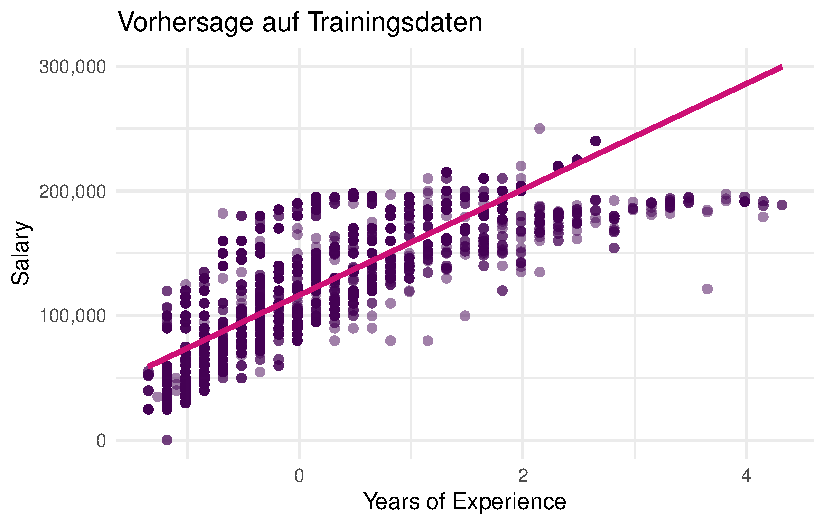
\includegraphics{main_doc_files/figure-pdf/unnamed-chunk-112-1.pdf}

}

\end{figure}

\begin{Shaded}
\begin{Highlighting}[]
\FunctionTok{ggplot}\NormalTok{(test\_data, }\FunctionTok{aes}\NormalTok{(}\AttributeTok{x =}\NormalTok{ Years.Of.Experience, }\AttributeTok{y =}\NormalTok{ Salary)) }\SpecialCharTok{+}
  \FunctionTok{geom\_point}\NormalTok{(}\AttributeTok{color =} \FunctionTok{viridis}\NormalTok{(}\FloatTok{0.50}\NormalTok{), }\AttributeTok{alpha =} \FloatTok{0.5}\NormalTok{) }\SpecialCharTok{+}
  \FunctionTok{geom\_line}\NormalTok{(}\FunctionTok{aes}\NormalTok{(}\AttributeTok{y =}\NormalTok{ pred\_test), }\AttributeTok{color =} \StringTok{"deeppink3"}\NormalTok{, }\AttributeTok{size =} \DecValTok{1}\NormalTok{) }\SpecialCharTok{+}
  \FunctionTok{labs}\NormalTok{(}\AttributeTok{title =} \StringTok{"Vorhersage auf Testdaten"}\NormalTok{,}
       \AttributeTok{x =} \StringTok{"Years of Experience"}\NormalTok{,}
       \AttributeTok{y =} \StringTok{"Salary"}\NormalTok{) }\SpecialCharTok{+}
  \FunctionTok{scale\_color\_identity}\NormalTok{() }\SpecialCharTok{+}
  \FunctionTok{scale\_y\_continuous}\NormalTok{(}\AttributeTok{labels =}\NormalTok{ scales}\SpecialCharTok{::}\NormalTok{comma) }\SpecialCharTok{+}
  \FunctionTok{theme\_minimal}\NormalTok{()}
\end{Highlighting}
\end{Shaded}

\begin{figure}[H]

{\centering 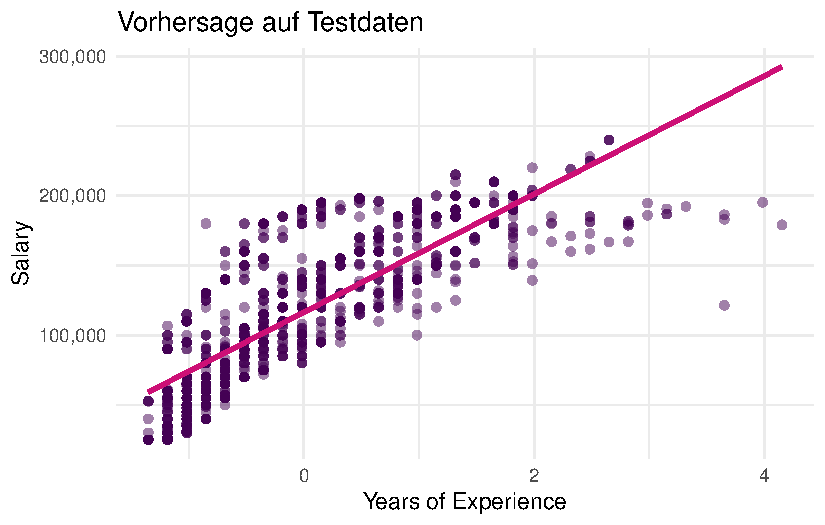
\includegraphics{main_doc_files/figure-pdf/unnamed-chunk-112-2.pdf}

}

\end{figure}

Anhand der zwei Grafiken ist zu erkennen, dass die unterschiedlichen
Werte bei der Vorhersage der Trainingsdaten deutlich dichter zusammen
liegen, als bei den Testdaten. Trotzdem sind die beiden Grafiken gleich,
was den Trend angeht. Dies ist Mithilfe der Regressionsgeraden zu
erkennen.

\hypertarget{fehler}{%
\subsubsection{7.1.5.: Fehler}\label{fehler}}

Mithilfe der ``rmse''-Funktion, wird die Quadratwurzel aus dem
Durchschnitt der quadrierten Differenzen zwischen den vorhergesagten und
den tatsächlichen Werten.

Trainingsfehler:

\begin{Shaded}
\begin{Highlighting}[]
\FunctionTok{rmse}\NormalTok{(compare\_train, Salary, pred\_train)}
\end{Highlighting}
\end{Shaded}

\begin{verbatim}
# A tibble: 1 x 3
  .metric .estimator .estimate
  <chr>   <chr>          <dbl>
1 rmse    standard      30725.
\end{verbatim}

Die durchschnittliche Abweichung beträgt rund 31.000.

Testfehler:

\begin{Shaded}
\begin{Highlighting}[]
\FunctionTok{rmse}\NormalTok{(compare\_test, Salary, pred\_test)}
\end{Highlighting}
\end{Shaded}

\begin{verbatim}
# A tibble: 1 x 3
  .metric .estimator .estimate
  <chr>   <chr>          <dbl>
1 rmse    standard      30764.
\end{verbatim}

Auch hier beträgt die durchschnittliche Abweichung rund 31.000.

Zur Einordnung der Fehler wird die Verteilung von Gehalt angesehen:

\begin{Shaded}
\begin{Highlighting}[]
\FunctionTok{describe}\NormalTok{(filtered\_data5, Salary)}
\end{Highlighting}
\end{Shaded}

\begin{verbatim}
variable = Salary
type     = double
na       = 0 of 6 398 (0%)
unique   = 432
min|max  = 550 | 250 000
q05|q95  = 35 000 | 195 000
q25|q75  = 70 000 | 160 000
median   = 120 000
mean     = 116 787.2
\end{verbatim}

Verteilung von Arbeitserfahrung:

\begin{Shaded}
\begin{Highlighting}[]
\FunctionTok{describe}\NormalTok{(filtered\_data5, Years.Of.Experience)}
\end{Highlighting}
\end{Shaded}

\begin{verbatim}
variable = Years.Of.Experience
type     = double
na       = 0 of 6 398 (0%)
unique   = 37
min|max  = 0 | 34
q05|q95  = 1 | 19
q25|q75  = 3 | 12
median   = 7
mean     = 8.101751
\end{verbatim}

\hypertarget{residuen}{%
\subsubsection{7.1.6.: Residuen}\label{residuen}}

Residuen (auch Fehler oder Residuen genannt) sind die Unterschiede
zwischen den beobachteten Werten und den vorhergesagten Werten in einem
Regressionsmodell. Sie stellen die Abweichungen zwischen den
tatsächlichen Daten und den durch das Modell vorhergesagten Werten dar.
Idealerweise sollten die Residuen normalverteilt sein, um
sicherzustellen, dass das Regressionsmodell angemessen ist.

Es ist üblich, die Residuen sowohl für Trainingsdaten als auch für
Testdaten zu überprüfen, um die Leistung des Modells auf beiden
Datensätzen zu evaluieren. Hier sind einige Gründe, warum es wichtig
ist, die Residuen auf beiden Datensätzen zu betrachten:

\begin{enumerate}
\def\labelenumi{\arabic{enumi}.}
\item
  \textbf{Trainingsdaten:}

  \begin{itemize}
  \tightlist
  \item
    Die Residuen der Trainingsdaten geben Ihnen einen Einblick in die
    Leistung des Modells auf den Daten, auf denen es trainiert wurde.
    Wenn die Residuen auf den Trainingsdaten ungewöhnliche Muster
    aufweisen, kann dies auf Modellprobleme oder Overfitting hinweisen.
  \end{itemize}
\item
  \textbf{Testdaten:}

  \begin{itemize}
  \tightlist
  \item
    Die Residuen der Testdaten ermöglichen es Ihnen, die
    Generalisierungsfähigkeit des Modells auf neuen, nicht trainierten
    Daten zu überprüfen. Ein Modell kann auf den Trainingsdaten gut
    funktionieren, aber die Residuen auf den Testdaten können Ihnen
    sagen, wie gut es sich auf unbekannte Daten verallgemeinert.
  \end{itemize}
\end{enumerate}

Nun werden die Risiduen mit der ``augment()''-Funktion auf die
Trainings-, sowie Testdaten abgerufen. Anschließend werden Sie
ausgegeben.

\begin{Shaded}
\begin{Highlighting}[]
\NormalTok{residuals\_train }\OtherTok{\textless{}{-}} \FunctionTok{augment}\NormalTok{(lm\_fit, }\AttributeTok{new\_data =}\NormalTok{ fd5\_train) }\SpecialCharTok{\%\textgreater{}\%} \FunctionTok{select}\NormalTok{(.resid)}

\NormalTok{residuals\_test }\OtherTok{\textless{}{-}} \FunctionTok{augment}\NormalTok{(lm\_fit, }\AttributeTok{new\_data =}\NormalTok{ fd5\_test) }\SpecialCharTok{\%\textgreater{}\%} \FunctionTok{select}\NormalTok{(.resid)}

\FunctionTok{print}\NormalTok{(residuals\_train)}
\end{Highlighting}
\end{Shaded}

\begin{verbatim}
# A tibble: 5,117 x 1
    .resid
     <dbl>
 1  -6278.
 2   9594.
 3   4594.
 4 -11278.
 5   1658.
 6  -6278.
 7 -11278.
 8   9594.
 9  -3342.
10  -6278.
# i 5,107 more rows
\end{verbatim}

\begin{Shaded}
\begin{Highlighting}[]
\FunctionTok{print}\NormalTok{(residuals\_test)}
\end{Highlighting}
\end{Shaded}

\begin{verbatim}
# A tibble: 1,281 x 1
   .resid
    <dbl>
 1  9594.
 2 -3342.
 3 -6278.
 4 23402.
 5 28402.
 6  7530.
 7 -3342.
 8 28402.
 9  9594.
10 -3342.
# i 1,271 more rows
\end{verbatim}

Anschließend werden nun die Risiduen in einem Histogramm ausgegeben,
nachdem Sie z-skaliert wurden.

Histogramm der Risiduen der Trainingsdaten:

\begin{Shaded}
\begin{Highlighting}[]
\NormalTok{residuals\_train}\SpecialCharTok{$}\NormalTok{standardized\_resid }\OtherTok{\textless{}{-}} \FunctionTok{scale}\NormalTok{(residuals\_train}\SpecialCharTok{$}\NormalTok{.resid)}

\FunctionTok{ggplot}\NormalTok{(}\AttributeTok{data =}\NormalTok{ residuals\_train, }\FunctionTok{aes}\NormalTok{(}\AttributeTok{x =}\NormalTok{ standardized\_resid)) }\SpecialCharTok{+}
  \FunctionTok{geom\_histogram}\NormalTok{(}\AttributeTok{binwidth =} \FloatTok{0.5}\NormalTok{, }\AttributeTok{fill =} \FunctionTok{viridis}\NormalTok{(}\DecValTok{1}\NormalTok{), }\AttributeTok{color =} \StringTok{"black"}\NormalTok{, }\AttributeTok{alpha =} \FloatTok{0.7}\NormalTok{) }\SpecialCharTok{+}
  \FunctionTok{labs}\NormalTok{(}\AttributeTok{title =} \StringTok{"Histogramm der standardisierten Residuen"}\NormalTok{,}
       \AttributeTok{x =} \StringTok{"Standardisierte Residuen"}\NormalTok{,}
       \AttributeTok{y =} \StringTok{"Häufigkeit"}\NormalTok{) }\SpecialCharTok{+}
  \FunctionTok{scale\_fill\_viridis}\NormalTok{() }\SpecialCharTok{+}  
  \FunctionTok{theme\_minimal}\NormalTok{()}
\end{Highlighting}
\end{Shaded}

\begin{figure}[H]

{\centering \includegraphics{main_doc_files/figure-pdf/unnamed-chunk-119-1.pdf}

}

\end{figure}

Zu erkennen ist, dass die Werte zwischen 2 und -2 am häufigsten
vertreten sind.

Histogramm der Risiduen der Testdaten:

\begin{Shaded}
\begin{Highlighting}[]
\NormalTok{residuals\_test}\SpecialCharTok{$}\NormalTok{standardized\_resid }\OtherTok{\textless{}{-}} \FunctionTok{scale}\NormalTok{(residuals\_test}\SpecialCharTok{$}\NormalTok{.resid)}

\FunctionTok{ggplot}\NormalTok{(}\AttributeTok{data =}\NormalTok{ residuals\_test, }\FunctionTok{aes}\NormalTok{(}\AttributeTok{x =}\NormalTok{ standardized\_resid)) }\SpecialCharTok{+}
  \FunctionTok{geom\_histogram}\NormalTok{(}\AttributeTok{binwidth =} \FloatTok{0.5}\NormalTok{, }\AttributeTok{fill =} \FunctionTok{viridis}\NormalTok{(}\DecValTok{1}\NormalTok{), }\AttributeTok{color =} \StringTok{"black"}\NormalTok{, }\AttributeTok{alpha =} \FloatTok{0.7}\NormalTok{) }\SpecialCharTok{+}
  \FunctionTok{labs}\NormalTok{(}\AttributeTok{title =} \StringTok{"Histogramm der standardisierten Residuen"}\NormalTok{,}
       \AttributeTok{x =} \StringTok{"Standardisierte Residuen"}\NormalTok{,}
       \AttributeTok{y =} \StringTok{"Häufigkeit"}\NormalTok{) }\SpecialCharTok{+}
  \FunctionTok{scale\_fill\_viridis}\NormalTok{() }\SpecialCharTok{+}
  \FunctionTok{theme\_minimal}\NormalTok{()}
\end{Highlighting}
\end{Shaded}

\begin{figure}[H]

{\centering \includegraphics{main_doc_files/figure-pdf/unnamed-chunk-120-1.pdf}

}

\end{figure}

Auch hier sind die Risiduen zwischen 2 und -2 am häufigsten.

Aus den beiden Histogrammen geht also hervor, dass die Abweichungen
zwischen den vorhergesagten Werten und tatsächlichen Werten nicht
wirklich groß sind.

\hypertarget{q-q-plot}{%
\subsubsection{7.1.7.: Q-Q-Plot}\label{q-q-plot}}

Das ``Quantil-Quantil-Diagramm'' überprüft Risiduen auf Ihre
Normalverteilung. Hierbei werden die Quantile der standartisierten
Risiduen gegen die QUantile der Normalverteilung gestellt. Im Normalfall
sollten die Punkte entlang der Diagonale (x=y) streuen.

QQ-Plot für der Risiduen für die Trainingsdaten:

\begin{Shaded}
\begin{Highlighting}[]
\FunctionTok{ggplot}\NormalTok{(}\AttributeTok{data =}\NormalTok{ residuals\_train, }\FunctionTok{aes}\NormalTok{(}\AttributeTok{sample =}\NormalTok{ standardized\_resid)) }\SpecialCharTok{+}
  \FunctionTok{stat\_qq}\NormalTok{(}\AttributeTok{distribution =}\NormalTok{ qnorm, }\AttributeTok{dparams =} \FunctionTok{list}\NormalTok{(}\AttributeTok{mean =} \DecValTok{0}\NormalTok{, }\AttributeTok{sd =} \DecValTok{1}\NormalTok{), }\AttributeTok{color =} \FunctionTok{viridis}\NormalTok{(}\DecValTok{1}\NormalTok{)) }\SpecialCharTok{+}
  \FunctionTok{geom\_abline}\NormalTok{(}\AttributeTok{intercept =} \DecValTok{0}\NormalTok{, }\AttributeTok{slope =} \DecValTok{1}\NormalTok{, }\AttributeTok{linetype =} \StringTok{"dashed"}\NormalTok{, }\AttributeTok{color =} \StringTok{"black"}\NormalTok{) }\SpecialCharTok{+}
  \FunctionTok{labs}\NormalTok{(}\AttributeTok{title =} \StringTok{"QQ{-}Plot der standardisierten Residuen"}\NormalTok{,}
       \AttributeTok{x =} \StringTok{"Quantile der Normalverteilung"}\NormalTok{,}
       \AttributeTok{y =} \StringTok{"Quantile der Residuen"}\NormalTok{) }\SpecialCharTok{+}
  \FunctionTok{scale\_color\_viridis}\NormalTok{() }\SpecialCharTok{+} 
  \FunctionTok{theme\_minimal}\NormalTok{()}
\end{Highlighting}
\end{Shaded}

\begin{figure}[H]

{\centering \includegraphics{main_doc_files/figure-pdf/unnamed-chunk-121-1.pdf}

}

\end{figure}

QQ-Plot für der Risiduen für die Testdaten:

\begin{Shaded}
\begin{Highlighting}[]
\NormalTok{residuals\_test}\SpecialCharTok{$}\NormalTok{standardized\_resid }\OtherTok{\textless{}{-}} \FunctionTok{scale}\NormalTok{(residuals\_test}\SpecialCharTok{$}\NormalTok{.resid)}
\FunctionTok{ggplot}\NormalTok{(}\AttributeTok{data =}\NormalTok{ residuals\_test, }\FunctionTok{aes}\NormalTok{(}\AttributeTok{sample =}\NormalTok{ standardized\_resid)) }\SpecialCharTok{+}
  \FunctionTok{stat\_qq}\NormalTok{(}\AttributeTok{distribution =}\NormalTok{ qnorm, }\AttributeTok{dparams =} \FunctionTok{list}\NormalTok{(}\AttributeTok{mean =} \DecValTok{0}\NormalTok{, }\AttributeTok{sd =} \DecValTok{1}\NormalTok{), }\AttributeTok{color =} \FunctionTok{viridis}\NormalTok{(}\DecValTok{1}\NormalTok{)) }\SpecialCharTok{+}
  \FunctionTok{geom\_abline}\NormalTok{(}\AttributeTok{intercept =} \DecValTok{0}\NormalTok{, }\AttributeTok{slope =} \DecValTok{1}\NormalTok{, }\AttributeTok{linetype =} \StringTok{"dashed"}\NormalTok{, }\AttributeTok{color =} \StringTok{"black"}\NormalTok{) }\SpecialCharTok{+}
  \FunctionTok{labs}\NormalTok{(}\AttributeTok{title =} \StringTok{"QQ{-}Plot der standardisierten Residuen"}\NormalTok{,}
       \AttributeTok{x =} \StringTok{"Quantile der Normalverteilung"}\NormalTok{,}
       \AttributeTok{y =} \StringTok{"Quantile der Residuen"}\NormalTok{) }\SpecialCharTok{+}
  \FunctionTok{scale\_color\_viridis}\NormalTok{() }\SpecialCharTok{+} 
  \FunctionTok{theme\_minimal}\NormalTok{()}
\end{Highlighting}
\end{Shaded}

\begin{figure}[H]

{\centering \includegraphics{main_doc_files/figure-pdf/unnamed-chunk-122-1.pdf}

}

\end{figure}

Die beiden Q-Q-Plots bilden die ``Ausreißer'' vom Gehalt nach oben oder
unten, entlang der 45-Grad-Linie ab, welche bereits im ersten Diagramm
von 7.1 zu sehen sind. Es ist zu erkennen, dass die Risiduen nicht
perfekt normalverteilt sind. Es besteht die Möglichkeit, dass
esDatenpunkte gibt, welche die Risiduen beeinflussen. Aufgrund der
explorativen Datenanalyse ist bereits bekannt, das Jobs mit hoher
Berufserfahrung oft Führungsverantwortung beinhalten, welche nochmals
zusätzlich monetär honoriert wird. Rechts oben im Graph ist eine flache
Linie zu erkennen. Diese deutet auf einen Gehaltscap hin. Die
``Ausreißer'' am unteren Ende lassen sichh durch z.B Einstiegsjobs,
sowie Niedriglohnjobs ohne Hochschulabschluss erläutern. Desweiteren ist
noch anzumerken, dass Ausbildungsberufe nicht beachtet werden.

\hypertarget{mehrfache-lineare-regression}{%
\subsection{7.2.: Mehrfache Lineare
Regression}\label{mehrfache-lineare-regression}}

In dem folgenden Absatz wird eine lineare mehrfache Regression
durchgeführt.

\hypertarget{vorbereitung-1}{%
\subsubsection{7.2.1.: Vorbereitung}\label{vorbereitung-1}}

Zunächst muss eine gewisse Vorbereitung getroffen werden.

In diesem Fall wird einmal der Adjusted R-Squad-Wert berechnet. Dieser
gibt an wie gut eine Variable, in diesem Fall ``Years of Experience''
die Variationen in der abhängigen Variable '' Salary'' in Ihrem Modell
erklärt. Dies geschieht unter der Berücksichtigung der Anzahl von
unabhängigen Variablen.

\begin{Shaded}
\begin{Highlighting}[]
\NormalTok{linear\_model }\OtherTok{\textless{}{-}} \FunctionTok{lm}\NormalTok{(Salary }\SpecialCharTok{\textasciitilde{}}\NormalTok{ Years.Of.Experience, }\AttributeTok{data =}\NormalTok{ filtered\_data3)}

\NormalTok{adjusted\_r\_squared }\OtherTok{\textless{}{-}} \FunctionTok{summary}\NormalTok{(linear\_model)}\SpecialCharTok{$}\NormalTok{adj.r.squared}

\FunctionTok{cat}\NormalTok{(}\StringTok{"Adjusted R{-}squared:"}\NormalTok{, adjusted\_r\_squared, }\StringTok{"}\SpecialCharTok{\textbackslash{}n}\StringTok{"}\NormalTok{)}
\end{Highlighting}
\end{Shaded}

\begin{verbatim}
Adjusted R-squared: 0.5713572 
\end{verbatim}

Der Adjusted R-squared-Wert liegt zwischen 0 und 1. In diesem Fall
bedeutet 0.5713572, dass etwa 57,14\% der Variationen in der abhängigen
Variable ``Salary'' durch die unabhängige Variable
``Years.Of.Experience'' im Modell erklärt werden können. Ein höherer
Wert wäre Wünschenswert.

Nun werden Streudiagramme mit einer glättenden Funktion erstellt.
Hierbei werden 3 Diagramme erstellt, wobei mit unterschiedlichen
Potenzen gerechnet wird.

\begin{Shaded}
\begin{Highlighting}[]
\FunctionTok{library}\NormalTok{(ggplot2)}
\FunctionTok{ggplot}\NormalTok{(}\AttributeTok{data =}\NormalTok{ filtered\_data, }\FunctionTok{aes}\NormalTok{(}\AttributeTok{x =}\NormalTok{ Years.Of.Experience, }\AttributeTok{y =}\NormalTok{ Salary)) }\SpecialCharTok{+}
  \FunctionTok{geom\_point}\NormalTok{() }\SpecialCharTok{+}
  \FunctionTok{geom\_smooth}\NormalTok{(}\AttributeTok{method =} \StringTok{"lm"}\NormalTok{, }\AttributeTok{formula =}\NormalTok{ y }\SpecialCharTok{\textasciitilde{}} \FunctionTok{poly}\NormalTok{(x, }\DecValTok{2}\NormalTok{), }\AttributeTok{se =} \ConstantTok{FALSE}\NormalTok{)}
\end{Highlighting}
\end{Shaded}

\begin{figure}[H]

{\centering \includegraphics{main_doc_files/figure-pdf/unnamed-chunk-124-1.pdf}

}

\end{figure}

\begin{Shaded}
\begin{Highlighting}[]
\FunctionTok{library}\NormalTok{(ggplot2)}
\FunctionTok{ggplot}\NormalTok{(}\AttributeTok{data =}\NormalTok{ filtered\_data, }\FunctionTok{aes}\NormalTok{(}\AttributeTok{x =}\NormalTok{ Years.Of.Experience, }\AttributeTok{y =}\NormalTok{ Salary)) }\SpecialCharTok{+}
  \FunctionTok{geom\_point}\NormalTok{() }\SpecialCharTok{+}
  \FunctionTok{geom\_smooth}\NormalTok{(}\AttributeTok{method =} \StringTok{"lm"}\NormalTok{, }\AttributeTok{formula =}\NormalTok{ y }\SpecialCharTok{\textasciitilde{}} \FunctionTok{poly}\NormalTok{(x, }\DecValTok{3}\NormalTok{), }\AttributeTok{se =} \ConstantTok{FALSE}\NormalTok{)}
\end{Highlighting}
\end{Shaded}

\begin{figure}[H]

{\centering \includegraphics{main_doc_files/figure-pdf/unnamed-chunk-125-1.pdf}

}

\end{figure}

\begin{Shaded}
\begin{Highlighting}[]
\FunctionTok{library}\NormalTok{(ggplot2)}
\FunctionTok{ggplot}\NormalTok{(}\AttributeTok{data =}\NormalTok{ filtered\_data, }\FunctionTok{aes}\NormalTok{(}\AttributeTok{x =}\NormalTok{ Years.Of.Experience, }\AttributeTok{y =}\NormalTok{ Salary)) }\SpecialCharTok{+}
  \FunctionTok{geom\_point}\NormalTok{() }\SpecialCharTok{+}
  \FunctionTok{geom\_smooth}\NormalTok{(}\AttributeTok{method =} \StringTok{"lm"}\NormalTok{, }\AttributeTok{formula =}\NormalTok{ y }\SpecialCharTok{\textasciitilde{}} \FunctionTok{poly}\NormalTok{(x, }\DecValTok{4}\NormalTok{), }\AttributeTok{se =} \ConstantTok{FALSE}\NormalTok{)}
\end{Highlighting}
\end{Shaded}

\begin{figure}[H]

{\centering \includegraphics{main_doc_files/figure-pdf/unnamed-chunk-126-1.pdf}

}

\end{figure}

Aufgrund der Kurve wurde sich entschieden eine weitere Variable, sowie
die Potenzen 2, 3 und 4 von '' Years of Experience'' hinzuzufügen und
anschließend je 3 unterschiedliche Regressionen durchzuführen.
Anschließend wird dann geschaut, wie akkurat sich das Modell auf die
Testdaten mit der jeweiligen Potenz verhält.

Da Age zwar einen hohen Korrelationswert hat aber auch mit den
Years.Of.Experience einhergeht nehmen wir diesen Wert nicht, sondern
stattdessen das Education.Level. Dies wird in den nächsten Absätzen
behandelt.

\hypertarget{korrelationen-2}{%
\subsubsection{7.2.2.: Korrelationen}\label{korrelationen-2}}

Um die Korrelation von dem ``Education Level'' zu berechnen müssen die
Werte erst von kategorisch zu nummerisch transformiert werden.

\begin{Shaded}
\begin{Highlighting}[]
\NormalTok{filtered\_data}\SpecialCharTok{$}\NormalTok{Education.Level }\OtherTok{\textless{}{-}} \FunctionTok{as.numeric}\NormalTok{(}\FunctionTok{as.character}\NormalTok{(filtered\_data}\SpecialCharTok{$}\NormalTok{Education.Level))}

\FunctionTok{str}\NormalTok{(filtered\_data}\SpecialCharTok{$}\NormalTok{Education.Level)}
\end{Highlighting}
\end{Shaded}

\begin{verbatim}
 num [1:6398] 2 1 2 2 1 2 2 2 1 1 ...
\end{verbatim}

\begin{Shaded}
\begin{Highlighting}[]
\NormalTok{correlations }\OtherTok{\textless{}{-}} \FunctionTok{cor}\NormalTok{(filtered\_data[}\FunctionTok{c}\NormalTok{(}\StringTok{"Salary"}\NormalTok{, }\StringTok{"Age"}\NormalTok{, }\StringTok{"Years.Of.Experience"}\NormalTok{, }\StringTok{"Education.Level"}\NormalTok{)])}

\FunctionTok{print}\NormalTok{(correlations)}
\end{Highlighting}
\end{Shaded}

\begin{verbatim}
                       Salary       Age Years.Of.Experience Education.Level
Salary              1.0000000 0.7291603           0.8103542       0.6374551
Age                 0.7291603 1.0000000           0.9363709       0.5965278
Years.Of.Experience 0.8103542 0.9363709           1.0000000       0.6105127
Education.Level     0.6374551 0.5965278           0.6105127       1.0000000
\end{verbatim}

Nun ist zu erkennen, dass zwischen dem Education Level und Salary eine
Korrelation von 0.63 vorliegt. Zwischen dem Alter und den Bildungsniveau
liegt dann eine Korrelation von 0.59. und dem '' Years of Experience''
eine Korrelation von 0.61.

Es ist also zu erkennen, dass Die Korrelationen zwischen dem
Bildungsniveau und den anderen stets relativ hoch ist.

\hypertarget{datenaufbereitung-2}{%
\subsubsection{7.2.3.: Datenaufbereitung}\label{datenaufbereitung-2}}

Für die Regressionen sind nur die ``Salary, Years of Experience,
Education Level'' relevant, also werden nur sie in den nen Datensatz
geschrieben:

\begin{Shaded}
\begin{Highlighting}[]
\NormalTok{filtered\_data6 }\OtherTok{\textless{}{-}}\NormalTok{ filtered\_data }\SpecialCharTok{\%\textgreater{}\%}
  \FunctionTok{select}\NormalTok{(Salary, Years.Of.Experience, Education.Level)}
\end{Highlighting}
\end{Shaded}

Anschließend werden die ``Years of Experience'' potenziert und
ausgegeben:

\begin{Shaded}
\begin{Highlighting}[]
\NormalTok{filtered\_data6 }\OtherTok{\textless{}{-}}\NormalTok{ filtered\_data6 }\SpecialCharTok{\%\textgreater{}\%}
  \FunctionTok{mutate}\NormalTok{(}\AttributeTok{Years.Of.Experience\_Squared =}\NormalTok{ Years.Of.Experience}\SpecialCharTok{\^{}}\DecValTok{2}\NormalTok{) }\SpecialCharTok{\%\textgreater{}\%}
  \FunctionTok{mutate}\NormalTok{(}\AttributeTok{Years.Of.Experience\_Cubed =}\NormalTok{ Years.Of.Experience}\SpecialCharTok{\^{}}\DecValTok{3}\NormalTok{) }\SpecialCharTok{\%\textgreater{}\%}
  \FunctionTok{mutate}\NormalTok{(}\AttributeTok{Years.Of.Experience\_Quartic =}\NormalTok{ Years.Of.Experience}\SpecialCharTok{\^{}}\DecValTok{4}\NormalTok{)}
\end{Highlighting}
\end{Shaded}

\begin{Shaded}
\begin{Highlighting}[]
\FunctionTok{head}\NormalTok{(filtered\_data6)}
\end{Highlighting}
\end{Shaded}

\begin{verbatim}
# A tibble: 6 x 6
  Salary Years.Of.Experience Education.Level Years.Of.Experience_Squared
   <dbl>               <dbl>           <dbl>                       <dbl>
1 110000                   5               2                          25
2  95000                   4               1                          16
3  90000                   3               2                           9
4  70000                   2               2                           4
5  60000                   1               1                           1
6  90000                   3               2                           9
# i 2 more variables: Years.Of.Experience_Cubed <dbl>,
#   Years.Of.Experience_Quartic <dbl>
\end{verbatim}

Nun wird wieder eine Z-Skalierung von ``filtered\_data6'' durchgeführt.

Hierzu wird zunächst eine Kopie des Datensatzes erstellt. Anschließend
werden dann die ``Years of Experience'' und das ``Education Level''
z-skaliert.

\begin{Shaded}
\begin{Highlighting}[]
\CommentTok{\# Erstellen Sie eine Kopie von filtered\_data6}
\NormalTok{filtered\_data6\_z }\OtherTok{\textless{}{-}}\NormalTok{ filtered\_data6}

\CommentTok{\# Z{-}Skalierung für Years.Of.Experience und Education.Level in filtered\_data6\_z durchführen}
\NormalTok{filtered\_data6\_z }\OtherTok{\textless{}{-}}\NormalTok{ filtered\_data6\_z }\SpecialCharTok{\%\textgreater{}\%}
  \FunctionTok{mutate}\NormalTok{(}
    \AttributeTok{Years.Of.Experience =} \FunctionTok{scale}\NormalTok{(Years.Of.Experience),}
    \AttributeTok{Education.Level =} \FunctionTok{scale}\NormalTok{(Education.Level)}
\NormalTok{  )}
\end{Highlighting}
\end{Shaded}

Ergebnis der Z-Skalierung:

\begin{Shaded}
\begin{Highlighting}[]
\FunctionTok{head}\NormalTok{(filtered\_data6\_z)}
\end{Highlighting}
\end{Shaded}

\begin{verbatim}
# A tibble: 6 x 6
  Salary Years.Of.Experience[,1] Education.Level[,1] Years.Of.Experience_Squared
   <dbl>                   <dbl>               <dbl>                       <dbl>
1 110000                  -0.517               0.411                          25
2  95000                  -0.684              -0.724                          16
3  90000                  -0.851               0.411                           9
4  70000                  -1.02                0.411                           4
5  60000                  -1.18               -0.724                           1
6  90000                  -0.851               0.411                           9
# i 2 more variables: Years.Of.Experience_Cubed <dbl>,
#   Years.Of.Experience_Quartic <dbl>
\end{verbatim}

Nun wird die Standardabweichung der Berufserfahrung überprüft.

\begin{Shaded}
\begin{Highlighting}[]
\FunctionTok{sd}\NormalTok{(filtered\_data6\_z}\SpecialCharTok{$}\NormalTok{Years.Of.Experience)}
\end{Highlighting}
\end{Shaded}

\begin{verbatim}
[1] 1
\end{verbatim}

\begin{Shaded}
\begin{Highlighting}[]
\FunctionTok{sd}\NormalTok{(filtered\_data6\_z}\SpecialCharTok{$}\NormalTok{Education.Level)}
\end{Highlighting}
\end{Shaded}

\begin{verbatim}
[1] 1
\end{verbatim}

Bei beiden liegt eine Abweichung von 1 vor.

Um eine lineare Regression durchzuführen wird der Datensatz
filtered\_data\_z in Trainings- und Testdaten eingeteilt. Mithilfe der
Funktion ``set.seed(007)'' initialisiert den Zufallsgenerator mit einer
festen Zahl, um sicherzustellen, dass die Ergebnisse bei jedem Durchlauf
reproduzierbar sind. ``initial\_split'' teilt dann den Datensatz in
Tranings- und Testdaten. Der Parameter strata = Years.Of.Experience
sorgt dafür, dass die Daten nach dem Gehalts-Wert stratifiziert werden,
um sicherzustellen, dass die Trainings- und Testdaten eine ähnliche
Verteilung von Gehalts-Werten aufweisen. Da die Potenzen dieser Variable
alle in der selben Reihe stehen muss hier nichts verändert werden. Die
Funktion training() extrahiert die Trainingsdaten aus dem aufgeteilten
Datensatz, während testing() die Testdaten extrahiert.

\begin{Shaded}
\begin{Highlighting}[]
\FunctionTok{set.seed}\NormalTok{(}\DecValTok{007}\NormalTok{)  }
\NormalTok{filtered\_data6\_z }\OtherTok{\textless{}{-}} \FunctionTok{initial\_split}\NormalTok{(filtered\_data6\_z, }\AttributeTok{prop =} \FloatTok{0.8}\NormalTok{, }\AttributeTok{strata =}\NormalTok{ Years.Of.Experience)  }

\NormalTok{fd6\_train }\OtherTok{\textless{}{-}} \FunctionTok{training}\NormalTok{(filtered\_data6\_z)}
\NormalTok{fd6\_test }\OtherTok{\textless{}{-}} \FunctionTok{testing}\NormalTok{(filtered\_data6\_z)}
\end{Highlighting}
\end{Shaded}

\hypertarget{modell-initialisieren-1}{%
\subsubsection{7.2.3.: Modell
Initialisieren}\label{modell-initialisieren-1}}

Nun muss das Modell initialisert werden.

\begin{Shaded}
\begin{Highlighting}[]
\NormalTok{lm\_model2 }\OtherTok{\textless{}{-}} \FunctionTok{linear\_reg}\NormalTok{() }\SpecialCharTok{|\textgreater{}} \FunctionTok{set\_engine}\NormalTok{(}\StringTok{"lm"}\NormalTok{)}
\end{Highlighting}
\end{Shaded}

Lineare Regression mit 2er Potenz:

\begin{Shaded}
\begin{Highlighting}[]
\NormalTok{lm\_fit2 }\OtherTok{\textless{}{-}}\NormalTok{ lm\_model2 }\SpecialCharTok{|\textgreater{}} \FunctionTok{fit}\NormalTok{(Salary }\SpecialCharTok{\textasciitilde{}}\NormalTok{ Years.Of.Experience }\SpecialCharTok{+}\NormalTok{ Education.Level }\SpecialCharTok{+}\NormalTok{ Years.Of.Experience\_Squared, }\AttributeTok{data =}\NormalTok{ fd6\_train)}
\end{Highlighting}
\end{Shaded}

Lineare Regression mit 3er Potenz:

\begin{Shaded}
\begin{Highlighting}[]
\NormalTok{lm\_fit3 }\OtherTok{\textless{}{-}}\NormalTok{ lm\_model2 }\SpecialCharTok{|\textgreater{}} \FunctionTok{fit}\NormalTok{(Salary }\SpecialCharTok{\textasciitilde{}}\NormalTok{ Years.Of.Experience }\SpecialCharTok{+}\NormalTok{ Education.Level }\SpecialCharTok{+}\NormalTok{ Years.Of.Experience\_Cubed, }\AttributeTok{data =}\NormalTok{ fd6\_train)}
\end{Highlighting}
\end{Shaded}

Lineare Regression mit 3er Potenz:

\begin{Shaded}
\begin{Highlighting}[]
\NormalTok{lm\_fit4 }\OtherTok{\textless{}{-}}\NormalTok{ lm\_model2 }\SpecialCharTok{|\textgreater{}} \FunctionTok{fit}\NormalTok{(Salary }\SpecialCharTok{\textasciitilde{}}\NormalTok{ Years.Of.Experience }\SpecialCharTok{+}\NormalTok{ Education.Level }\SpecialCharTok{+}\NormalTok{ Years.Of.Experience\_Quartic, }\AttributeTok{data =}\NormalTok{ fd6\_train)}
\end{Highlighting}
\end{Shaded}

Zusammenfassung des Ergebnis (2er Potenz):

\begin{Shaded}
\begin{Highlighting}[]
\NormalTok{summary }\OtherTok{\textless{}{-}}\NormalTok{ lm\_fit2 }\SpecialCharTok{|\textgreater{}} \FunctionTok{extract\_fit\_engine}\NormalTok{() }\SpecialCharTok{|\textgreater{}} \FunctionTok{summary}\NormalTok{()}
\NormalTok{summary}
\end{Highlighting}
\end{Shaded}

\begin{verbatim}

Call:
stats::lm(formula = Salary ~ Years.Of.Experience + Education.Level + 
    Years.Of.Experience_Squared, data = data)

Residuals:
   Min     1Q Median     3Q    Max 
-83843 -18771  -3740  10782  90478 

Coefficients:
                              Estimate Std. Error t value Pr(>|t|)    
(Intercept)                 143592.201    882.844  162.65   <2e-16 ***
Years.Of.Experience          73825.758   1234.509   59.80   <2e-16 ***
Education.Level               6527.658    493.036   13.24   <2e-16 ***
Years.Of.Experience_Squared   -266.380      7.883  -33.79   <2e-16 ***
---
Signif. codes:  0 '***' 0.001 '**' 0.01 '*' 0.05 '.' 0.1 ' ' 1

Residual standard error: 26430 on 5113 degrees of freedom
Multiple R-squared:  0.7464,    Adjusted R-squared:  0.7463 
F-statistic:  5017 on 3 and 5113 DF,  p-value: < 2.2e-16
\end{verbatim}

Zusammenfassung des Ergebnis (3er Potenz):

\begin{Shaded}
\begin{Highlighting}[]
\CommentTok{\# Zusammenfassung der Regression}
\NormalTok{summary }\OtherTok{\textless{}{-}}\NormalTok{ lm\_fit3 }\SpecialCharTok{|\textgreater{}} \FunctionTok{extract\_fit\_engine}\NormalTok{() }\SpecialCharTok{|\textgreater{}} \FunctionTok{summary}\NormalTok{()}
\NormalTok{summary}
\end{Highlighting}
\end{Shaded}

\begin{verbatim}

Call:
stats::lm(formula = Salary ~ Years.Of.Experience + Education.Level + 
    Years.Of.Experience_Cubed, data = data)

Residuals:
   Min     1Q Median     3Q    Max 
-84267 -19790  -3860  11280  91008 

Coefficients:
                            Estimate Std. Error t value Pr(>|t|)    
(Intercept)                1.261e+05  4.865e+02  259.13   <2e-16 ***
Years.Of.Experience        5.507e+04  7.975e+02   69.05   <2e-16 ***
Education.Level            7.198e+03  4.977e+02   14.46   <2e-16 ***
Years.Of.Experience_Cubed -5.905e+00  1.911e-01  -30.90   <2e-16 ***
---
Signif. codes:  0 '***' 0.001 '**' 0.01 '*' 0.05 '.' 0.1 ' ' 1

Residual standard error: 26830 on 5113 degrees of freedom
Multiple R-squared:  0.7386,    Adjusted R-squared:  0.7385 
F-statistic:  4817 on 3 and 5113 DF,  p-value: < 2.2e-16
\end{verbatim}

Zusammenfassung des Ergebnis (4er Potenz):

\begin{Shaded}
\begin{Highlighting}[]
\NormalTok{summary }\OtherTok{\textless{}{-}}\NormalTok{ lm\_fit4 }\SpecialCharTok{|\textgreater{}} \FunctionTok{extract\_fit\_engine}\NormalTok{() }\SpecialCharTok{|\textgreater{}} \FunctionTok{summary}\NormalTok{()}
\NormalTok{summary}
\end{Highlighting}
\end{Shaded}

\begin{verbatim}

Call:
stats::lm(formula = Salary ~ Years.Of.Experience + Education.Level + 
    Years.Of.Experience_Quartic, data = data)

Residuals:
   Min     1Q Median     3Q    Max 
-82732 -19598  -3836  11803  90306 

Coefficients:
                              Estimate Std. Error t value Pr(>|t|)    
(Intercept)                  1.213e+05  4.176e+02  290.40   <2e-16 ***
Years.Of.Experience          4.801e+04  6.640e+02   72.31   <2e-16 ***
Education.Level              8.034e+03  5.007e+02   16.05   <2e-16 ***
Years.Of.Experience_Quartic -1.569e-01  5.637e-03  -27.83   <2e-16 ***
---
Signif. codes:  0 '***' 0.001 '**' 0.01 '*' 0.05 '.' 0.1 ' ' 1

Residual standard error: 27240 on 5113 degrees of freedom
Multiple R-squared:  0.7306,    Adjusted R-squared:  0.7305 
F-statistic:  4623 on 3 and 5113 DF,  p-value: < 2.2e-16
\end{verbatim}

Vorhersagen auf Trainings- und Testdatensatz (2er Potenz):

\begin{Shaded}
\begin{Highlighting}[]
\NormalTok{pred\_train2 }\OtherTok{\textless{}{-}} \FunctionTok{predict}\NormalTok{(lm\_fit2, }\AttributeTok{new\_data =}\NormalTok{ fd6\_train) }\SpecialCharTok{|\textgreater{}} \FunctionTok{rename}\NormalTok{(}\StringTok{"pred\_train2"} \OtherTok{=} \StringTok{".pred"}\NormalTok{)}
\NormalTok{pred\_test2 }\OtherTok{\textless{}{-}} \FunctionTok{predict}\NormalTok{(lm\_fit2, }\AttributeTok{new\_data =}\NormalTok{ fd6\_test) }\SpecialCharTok{|\textgreater{}}  \FunctionTok{rename}\NormalTok{(}\StringTok{"pred\_test2"} \OtherTok{=} \StringTok{".pred"}\NormalTok{)}

\NormalTok{compare\_train2 }\OtherTok{\textless{}{-}}\NormalTok{ fd5\_train }\SpecialCharTok{|\textgreater{}} 
  \FunctionTok{select}\NormalTok{(Salary) }\SpecialCharTok{|\textgreater{}} 
  \FunctionTok{bind\_cols}\NormalTok{(pred\_train2)}
\FunctionTok{head}\NormalTok{(compare\_train2)}
\end{Highlighting}
\end{Shaded}

\begin{verbatim}
# A tibble: 6 x 2
  Salary pred_train2
   <dbl>       <dbl>
1  60000      51180.
2  90000      81077.
3  85000      73668.
4  55000      51180.
5  75000      70099.
6  60000      51180.
\end{verbatim}

\begin{Shaded}
\begin{Highlighting}[]
\NormalTok{compare\_test2 }\OtherTok{\textless{}{-}}\NormalTok{ fd5\_test }\SpecialCharTok{|\textgreater{}} 
  \FunctionTok{select}\NormalTok{(Salary) }\SpecialCharTok{|\textgreater{}} 
  \FunctionTok{bind\_cols}\NormalTok{(pred\_test2)}
\FunctionTok{head}\NormalTok{(compare\_test2)}
\end{Highlighting}
\end{Shaded}

\begin{verbatim}
# A tibble: 6 x 2
  Salary pred_test2
   <dbl>      <dbl>
1  90000     81077.
2  70000     70099.
3  60000     58589.
4 125000    110813.
5 130000    110813.
6  95000     84113.
\end{verbatim}

Vorhersagen auf Trainings- und Testdatensatz (3er Potenz):

\begin{Shaded}
\begin{Highlighting}[]
\NormalTok{pred\_train3 }\OtherTok{\textless{}{-}} \FunctionTok{predict}\NormalTok{(lm\_fit3, }\AttributeTok{new\_data =}\NormalTok{ fd6\_train) }\SpecialCharTok{|\textgreater{}} \FunctionTok{rename}\NormalTok{(}\StringTok{"pred\_train3"} \OtherTok{=} \StringTok{".pred"}\NormalTok{)}
\NormalTok{pred\_test3 }\OtherTok{\textless{}{-}} \FunctionTok{predict}\NormalTok{(lm\_fit3, }\AttributeTok{new\_data =}\NormalTok{ fd6\_test) }\SpecialCharTok{|\textgreater{}}  \FunctionTok{rename}\NormalTok{(}\StringTok{"pred\_test3"} \OtherTok{=} \StringTok{".pred"}\NormalTok{)}

\NormalTok{compare\_train3 }\OtherTok{\textless{}{-}}\NormalTok{ fd6\_train }\SpecialCharTok{|\textgreater{}} 
  \FunctionTok{select}\NormalTok{(Salary) }\SpecialCharTok{|\textgreater{}} 
  \FunctionTok{bind\_cols}\NormalTok{(pred\_train3)}
\FunctionTok{head}\NormalTok{(compare\_train3)}
\end{Highlighting}
\end{Shaded}

\begin{verbatim}
# A tibble: 6 x 2
  Salary pred_train3
   <dbl>       <dbl>
1  60000      55650.
2  90000      82029.
3  85000      73860.
4  55000      55650.
5  75000      72960.
6  60000      55650.
\end{verbatim}

\begin{Shaded}
\begin{Highlighting}[]
\NormalTok{compare\_test3 }\OtherTok{\textless{}{-}}\NormalTok{ fd6\_test }\SpecialCharTok{|\textgreater{}} 
  \FunctionTok{select}\NormalTok{(Salary) }\SpecialCharTok{|\textgreater{}} 
  \FunctionTok{bind\_cols}\NormalTok{(pred\_test3)}
\FunctionTok{head}\NormalTok{(compare\_test3)}
\end{Highlighting}
\end{Shaded}

\begin{verbatim}
# A tibble: 6 x 2
  Salary pred_test3
   <dbl>      <dbl>
1  90000     82029.
2  70000     72960.
3  60000     63819.
4 125000    108458.
5 130000    108458.
6  95000     82823.
\end{verbatim}

Vorhersagen auf Trainings- und Testdatensatz (4er Potenz):

\begin{Shaded}
\begin{Highlighting}[]
\NormalTok{pred\_train4 }\OtherTok{\textless{}{-}} \FunctionTok{predict}\NormalTok{(lm\_fit4, }\AttributeTok{new\_data =}\NormalTok{ fd6\_train) }\SpecialCharTok{|\textgreater{}} \FunctionTok{rename}\NormalTok{(}\StringTok{"pred\_train4"} \OtherTok{=} \StringTok{".pred"}\NormalTok{)}
\NormalTok{pred\_test4 }\OtherTok{\textless{}{-}} \FunctionTok{predict}\NormalTok{(lm\_fit4, }\AttributeTok{new\_data =}\NormalTok{ fd6\_test) }\SpecialCharTok{|\textgreater{}}  \FunctionTok{rename}\NormalTok{(}\StringTok{"pred\_test4"} \OtherTok{=} \StringTok{".pred"}\NormalTok{)}

\NormalTok{compare\_train4 }\OtherTok{\textless{}{-}}\NormalTok{ fd6\_train }\SpecialCharTok{|\textgreater{}} 
  \FunctionTok{select}\NormalTok{(Salary) }\SpecialCharTok{|\textgreater{}} 
  \FunctionTok{bind\_cols}\NormalTok{(pred\_train4)}
\FunctionTok{head}\NormalTok{(compare\_train4)}
\end{Highlighting}
\end{Shaded}

\begin{verbatim}
# A tibble: 6 x 2
  Salary pred_train4
   <dbl>       <dbl>
1  60000      58600.
2  90000      83717.
3  85000      74598.
4  55000      58600.
5  75000      75721.
6  60000      58600.
\end{verbatim}

\begin{Shaded}
\begin{Highlighting}[]
\NormalTok{compare\_test4 }\OtherTok{\textless{}{-}}\NormalTok{ fd6\_test }\SpecialCharTok{|\textgreater{}} 
  \FunctionTok{select}\NormalTok{(Salary) }\SpecialCharTok{|\textgreater{}} 
  \FunctionTok{bind\_cols}\NormalTok{(pred\_test4)}
\FunctionTok{head}\NormalTok{(compare\_test4)}
\end{Highlighting}
\end{Shaded}

\begin{verbatim}
# A tibble: 6 x 2
  Salary pred_test4
   <dbl>      <dbl>
1  90000     83717.
2  70000     75721.
3  60000     67719.
4 125000    107542.
5 130000    107542.
6  95000     82576.
\end{verbatim}

\hypertarget{grafische-darstellung-1}{%
\subsubsection{7.2.4.: Grafische
Darstellung}\label{grafische-darstellung-1}}

In dem folgenden Absatz werden die unterschiedlichen Potenzen mithilfe
eines Vorhersage Plots grafisch dargestellt.

Hierzu wurde eine zusätzliche Quelle verwendet: (
\url{https://statologie.de/vorhergesagte-werte-plotten-r/})

Die folgenden Codechunks wird immer der gleiche Aufbau verwendet. Bloß
stets mit den unterschiedlichen Potenzen. Zunächst wird der Graph für
den Trainingdatensatz und anschließend für den Testdtaensatz erstellt.

2er Potenz:

\begin{Shaded}
\begin{Highlighting}[]
\FunctionTok{ggplot}\NormalTok{(compare\_train2, }\FunctionTok{aes}\NormalTok{(}\AttributeTok{x =}\NormalTok{ Salary, }\AttributeTok{y =}\NormalTok{ pred\_train2)) }\SpecialCharTok{+}
  \FunctionTok{geom\_point}\NormalTok{(}\AttributeTok{color =} \FunctionTok{viridis}\NormalTok{(}\FloatTok{0.50}\NormalTok{)) }\SpecialCharTok{+}
  \FunctionTok{geom\_abline}\NormalTok{(}\AttributeTok{intercept =} \DecValTok{0}\NormalTok{, }\AttributeTok{slope =} \DecValTok{1}\NormalTok{, }\AttributeTok{color =} \StringTok{"red"}\NormalTok{, }\AttributeTok{linetype =} \StringTok{"dashed"}\NormalTok{) }\SpecialCharTok{+}
  \FunctionTok{geom\_smooth}\NormalTok{(}\AttributeTok{method =} \StringTok{"lm"}\NormalTok{, }\AttributeTok{formula =}\NormalTok{ y }\SpecialCharTok{\textasciitilde{}} \FunctionTok{poly}\NormalTok{(x, }\DecValTok{3}\NormalTok{), }\AttributeTok{se =} \ConstantTok{FALSE}\NormalTok{) }\SpecialCharTok{+}
  \FunctionTok{labs}\NormalTok{(}\AttributeTok{title =} \StringTok{"Vorhersage{-}Plot für Trainingsdatensatz"}\NormalTok{,}
       \AttributeTok{x =} \StringTok{"Echte Salary{-}Werte"}\NormalTok{,}
       \AttributeTok{y =} \StringTok{"Vorhergesagte Salary{-}Werte"}\NormalTok{) }\SpecialCharTok{+}
  \FunctionTok{theme\_minimal}\NormalTok{()}
\end{Highlighting}
\end{Shaded}

\begin{figure}[H]

{\centering \includegraphics{main_doc_files/figure-pdf/unnamed-chunk-146-1.pdf}

}

\end{figure}

\begin{Shaded}
\begin{Highlighting}[]
\FunctionTok{ggplot}\NormalTok{(compare\_test2, }\FunctionTok{aes}\NormalTok{(}\AttributeTok{x =}\NormalTok{ Salary, }\AttributeTok{y =}\NormalTok{ pred\_test2)) }\SpecialCharTok{+}
  \FunctionTok{geom\_point}\NormalTok{(}\AttributeTok{color =} \FunctionTok{viridis}\NormalTok{(}\FloatTok{0.50}\NormalTok{)) }\SpecialCharTok{+}
  \FunctionTok{geom\_abline}\NormalTok{(}\AttributeTok{intercept =} \DecValTok{0}\NormalTok{, }\AttributeTok{slope =} \DecValTok{1}\NormalTok{, }\AttributeTok{color =} \StringTok{"red"}\NormalTok{, }\AttributeTok{linetype =} \StringTok{"dashed"}\NormalTok{) }\SpecialCharTok{+}
  \FunctionTok{geom\_smooth}\NormalTok{(}\AttributeTok{method =} \StringTok{"lm"}\NormalTok{, }\AttributeTok{formula =}\NormalTok{ y }\SpecialCharTok{\textasciitilde{}} \FunctionTok{poly}\NormalTok{(x, }\DecValTok{2}\NormalTok{), }\AttributeTok{se =} \ConstantTok{FALSE}\NormalTok{) }\SpecialCharTok{+}
  \FunctionTok{labs}\NormalTok{(}\AttributeTok{title =} \StringTok{"Vorhersage{-}Plot für Testdatensatz"}\NormalTok{,}
       \AttributeTok{x =} \StringTok{"Echte Salary{-}Werte"}\NormalTok{,}
       \AttributeTok{y =} \StringTok{"Vorhergesagte Salary{-}Werte"}\NormalTok{) }\SpecialCharTok{+}
  \FunctionTok{theme\_minimal}\NormalTok{()}
\end{Highlighting}
\end{Shaded}

\begin{figure}[H]

{\centering \includegraphics{main_doc_files/figure-pdf/unnamed-chunk-146-2.pdf}

}

\end{figure}

3er Potenz:

\begin{Shaded}
\begin{Highlighting}[]
\FunctionTok{ggplot}\NormalTok{(compare\_train3, }\FunctionTok{aes}\NormalTok{(}\AttributeTok{x =}\NormalTok{ Salary, }\AttributeTok{y =}\NormalTok{ pred\_train3)) }\SpecialCharTok{+}
  \FunctionTok{geom\_point}\NormalTok{(}\AttributeTok{color =} \FunctionTok{viridis}\NormalTok{(}\FloatTok{0.50}\NormalTok{)) }\SpecialCharTok{+}
  \FunctionTok{geom\_abline}\NormalTok{(}\AttributeTok{intercept =} \DecValTok{0}\NormalTok{, }\AttributeTok{slope =} \DecValTok{1}\NormalTok{, }\AttributeTok{color =} \StringTok{"red"}\NormalTok{, }\AttributeTok{linetype =} \StringTok{"dashed"}\NormalTok{) }\SpecialCharTok{+}
  \FunctionTok{geom\_smooth}\NormalTok{(}\AttributeTok{method =} \StringTok{"lm"}\NormalTok{, }\AttributeTok{formula =}\NormalTok{ y }\SpecialCharTok{\textasciitilde{}} \FunctionTok{poly}\NormalTok{(x, }\DecValTok{3}\NormalTok{), }\AttributeTok{se =} \ConstantTok{FALSE}\NormalTok{) }\SpecialCharTok{+}
  \FunctionTok{labs}\NormalTok{(}\AttributeTok{title =} \StringTok{"Vorhersage{-}Plot für Trainingsdatensatz"}\NormalTok{,}
       \AttributeTok{x =} \StringTok{"Echte Salary{-}Werte"}\NormalTok{,}
       \AttributeTok{y =} \StringTok{"Vorhergesagte Salary{-}Werte"}\NormalTok{) }\SpecialCharTok{+}
  \FunctionTok{theme\_minimal}\NormalTok{()}
\end{Highlighting}
\end{Shaded}

\begin{figure}[H]

{\centering \includegraphics{main_doc_files/figure-pdf/unnamed-chunk-147-1.pdf}

}

\end{figure}

\begin{Shaded}
\begin{Highlighting}[]
\FunctionTok{ggplot}\NormalTok{(compare\_test3, }\FunctionTok{aes}\NormalTok{(}\AttributeTok{x =}\NormalTok{ Salary, }\AttributeTok{y =}\NormalTok{ pred\_test3)) }\SpecialCharTok{+}
  \FunctionTok{geom\_point}\NormalTok{(}\AttributeTok{color =} \FunctionTok{viridis}\NormalTok{(}\FloatTok{0.50}\NormalTok{)) }\SpecialCharTok{+}
  \FunctionTok{geom\_abline}\NormalTok{(}\AttributeTok{intercept =} \DecValTok{0}\NormalTok{, }\AttributeTok{slope =} \DecValTok{1}\NormalTok{, }\AttributeTok{color =} \StringTok{"red"}\NormalTok{, }\AttributeTok{linetype =} \StringTok{"dashed"}\NormalTok{) }\SpecialCharTok{+}
  \FunctionTok{geom\_smooth}\NormalTok{(}\AttributeTok{method =} \StringTok{"lm"}\NormalTok{, }\AttributeTok{formula =}\NormalTok{ y }\SpecialCharTok{\textasciitilde{}} \FunctionTok{poly}\NormalTok{(x, }\DecValTok{3}\NormalTok{), }\AttributeTok{se =} \ConstantTok{FALSE}\NormalTok{) }\SpecialCharTok{+}
  \FunctionTok{labs}\NormalTok{(}\AttributeTok{title =} \StringTok{"Vorhersage{-}Plot für Testdatensatz"}\NormalTok{,}
       \AttributeTok{x =} \StringTok{"Echte Salary{-}Werte"}\NormalTok{,}
       \AttributeTok{y =} \StringTok{"Vorhergesagte Salary{-}Werte"}\NormalTok{) }\SpecialCharTok{+}
  \FunctionTok{theme\_minimal}\NormalTok{()}
\end{Highlighting}
\end{Shaded}

\begin{figure}[H]

{\centering \includegraphics{main_doc_files/figure-pdf/unnamed-chunk-147-2.pdf}

}

\end{figure}

4er Potenz:

\begin{Shaded}
\begin{Highlighting}[]
\FunctionTok{ggplot}\NormalTok{(compare\_train4, }\FunctionTok{aes}\NormalTok{(}\AttributeTok{x =}\NormalTok{ Salary, }\AttributeTok{y =}\NormalTok{ pred\_train4)) }\SpecialCharTok{+}
  \FunctionTok{geom\_point}\NormalTok{(}\AttributeTok{color =} \FunctionTok{viridis}\NormalTok{(}\FloatTok{0.50}\NormalTok{)) }\SpecialCharTok{+}
  \FunctionTok{geom\_abline}\NormalTok{(}\AttributeTok{intercept =} \DecValTok{0}\NormalTok{, }\AttributeTok{slope =} \DecValTok{1}\NormalTok{, }\AttributeTok{color =} \StringTok{"red"}\NormalTok{, }\AttributeTok{linetype =} \StringTok{"dashed"}\NormalTok{) }\SpecialCharTok{+}
  \FunctionTok{geom\_smooth}\NormalTok{(}\AttributeTok{method =} \StringTok{"lm"}\NormalTok{, }\AttributeTok{formula =}\NormalTok{ y }\SpecialCharTok{\textasciitilde{}} \FunctionTok{poly}\NormalTok{(x, }\DecValTok{3}\NormalTok{), }\AttributeTok{se =} \ConstantTok{FALSE}\NormalTok{) }\SpecialCharTok{+}
  \FunctionTok{labs}\NormalTok{(}\AttributeTok{title =} \StringTok{"Vorhersage{-}Plot für Trainingsdatensatz"}\NormalTok{,}
       \AttributeTok{x =} \StringTok{"Echte Salary{-}Werte"}\NormalTok{,}
       \AttributeTok{y =} \StringTok{"Vorhergesagte Salary{-}Werte"}\NormalTok{) }\SpecialCharTok{+}
  \FunctionTok{theme\_minimal}\NormalTok{()}
\end{Highlighting}
\end{Shaded}

\begin{figure}[H]

{\centering \includegraphics{main_doc_files/figure-pdf/unnamed-chunk-148-1.pdf}

}

\end{figure}

\begin{Shaded}
\begin{Highlighting}[]
\FunctionTok{ggplot}\NormalTok{(compare\_test4, }\FunctionTok{aes}\NormalTok{(}\AttributeTok{x =}\NormalTok{ Salary, }\AttributeTok{y =}\NormalTok{ pred\_test4)) }\SpecialCharTok{+}
  \FunctionTok{geom\_point}\NormalTok{(}\AttributeTok{color =} \FunctionTok{viridis}\NormalTok{(}\FloatTok{0.50}\NormalTok{)) }\SpecialCharTok{+}
  \FunctionTok{geom\_abline}\NormalTok{(}\AttributeTok{intercept =} \DecValTok{0}\NormalTok{, }\AttributeTok{slope =} \DecValTok{1}\NormalTok{, }\AttributeTok{color =} \StringTok{"red"}\NormalTok{, }\AttributeTok{linetype =} \StringTok{"dashed"}\NormalTok{) }\SpecialCharTok{+}
  \FunctionTok{geom\_smooth}\NormalTok{(}\AttributeTok{method =} \StringTok{"lm"}\NormalTok{, }\AttributeTok{formula =}\NormalTok{ y }\SpecialCharTok{\textasciitilde{}} \FunctionTok{poly}\NormalTok{(x, }\DecValTok{4}\NormalTok{), }\AttributeTok{se =} \ConstantTok{FALSE}\NormalTok{) }\SpecialCharTok{+}
  \FunctionTok{labs}\NormalTok{(}\AttributeTok{title =} \StringTok{"Vorhersage{-}Plot für Testdatensatz"}\NormalTok{,}
       \AttributeTok{x =} \StringTok{"Echte Salary{-}Werte"}\NormalTok{,}
       \AttributeTok{y =} \StringTok{"Vorhergesagte Salary{-}Werte"}\NormalTok{) }\SpecialCharTok{+}
  \FunctionTok{theme\_minimal}\NormalTok{()}
\end{Highlighting}
\end{Shaded}

\begin{figure}[H]

{\centering \includegraphics{main_doc_files/figure-pdf/unnamed-chunk-148-2.pdf}

}

\end{figure}

Es ist bereits eine Tendenz zu erkennen. Die 4er Potenz der
Berufserfahrung auf einer minimal genaueren Prognose bei den Testdaten,
im Vergleich zu der 2er und 3er Potenz, resultiert.

\hypertarget{fehler-1}{%
\subsubsection{7.2.5.: Fehler}\label{fehler-1}}

Auch hier werden die Potenzen einzeln und hintereinander mit dem
``rmse'' untersucht.

2er Potenz

Trainingsfehler:

\begin{Shaded}
\begin{Highlighting}[]
\FunctionTok{rmse}\NormalTok{(compare\_train2, Salary, pred\_train2)}
\end{Highlighting}
\end{Shaded}

\begin{verbatim}
# A tibble: 1 x 3
  .metric .estimator .estimate
  <chr>   <chr>          <dbl>
1 rmse    standard      26417.
\end{verbatim}

Testfehler:

\begin{Shaded}
\begin{Highlighting}[]
\FunctionTok{rmse}\NormalTok{(compare\_test2, Salary, pred\_test2)}
\end{Highlighting}
\end{Shaded}

\begin{verbatim}
# A tibble: 1 x 3
  .metric .estimator .estimate
  <chr>   <chr>          <dbl>
1 rmse    standard      26629.
\end{verbatim}

Es geht hervor, dass das Modell auf den Trainingsdaten besser perfomt
als auf den Testdaten.

Diese Tatsache weist auf Overfitting hin.

3er Potenz:

Trainingsfehler:

\begin{Shaded}
\begin{Highlighting}[]
\FunctionTok{rmse}\NormalTok{(compare\_train3, Salary, pred\_train3)}
\end{Highlighting}
\end{Shaded}

\begin{verbatim}
# A tibble: 1 x 3
  .metric .estimator .estimate
  <chr>   <chr>          <dbl>
1 rmse    standard      26820.
\end{verbatim}

Testfehler:

\begin{Shaded}
\begin{Highlighting}[]
\FunctionTok{rmse}\NormalTok{(compare\_test3, Salary, pred\_test3)}
\end{Highlighting}
\end{Shaded}

\begin{verbatim}
# A tibble: 1 x 3
  .metric .estimator .estimate
  <chr>   <chr>          <dbl>
1 rmse    standard      27035.
\end{verbatim}

Auch hier performt das Modell besser auf den Trainingsdaten. Dies weist
ebenfalls auf Overfitting hin.

4er Potenz:

Trainingsfehler:

\begin{Shaded}
\begin{Highlighting}[]
\FunctionTok{rmse}\NormalTok{(compare\_test4, Salary, pred\_test4)}
\end{Highlighting}
\end{Shaded}

\begin{verbatim}
# A tibble: 1 x 3
  .metric .estimator .estimate
  <chr>   <chr>          <dbl>
1 rmse    standard      27457.
\end{verbatim}

Testfehler:

\begin{Shaded}
\begin{Highlighting}[]
\FunctionTok{rmse}\NormalTok{(compare\_test4, Salary, pred\_test4)}
\end{Highlighting}
\end{Shaded}

\begin{verbatim}
# A tibble: 1 x 3
  .metric .estimator .estimate
  <chr>   <chr>          <dbl>
1 rmse    standard      27457.
\end{verbatim}

Auch wenn alle Modelle nur geringe Unterschiede aufweisen, performt
dieses auf den Trainingsdaten gleich wie auf den Testdaten. Demnach ist
es das präziseste Modell und wird als einziges weiter verwendet und
weiter verwendet.

Dies ließ sich bereits unter 7.2.1 erkennen, da das 3. Polynom das Geom
Smooth grafisch die beste Linie abgebildet hat.

Zur Einordnung der Fehler die Verteilung von Gehalt ansehen:

Verteilung von Gehalt:

\begin{Shaded}
\begin{Highlighting}[]
\FunctionTok{describe}\NormalTok{(filtered\_data5, Salary)}
\end{Highlighting}
\end{Shaded}

\begin{verbatim}
variable = Salary
type     = double
na       = 0 of 6 398 (0%)
unique   = 432
min|max  = 550 | 250 000
q05|q95  = 35 000 | 195 000
q25|q75  = 70 000 | 160 000
median   = 120 000
mean     = 116 787.2
\end{verbatim}

\hypertarget{residuen-1}{%
\subsubsection{7.2.6.: Residuen}\label{residuen-1}}

Der Aufbau, sowie die Definiton zu den Risiduen wurden bereits unter
7.1.6 aufgeführt.

Deswegen werden die Funktionen ebenfalls nicht erneut erläutert.

Es wird sich jediglich nur um die Ausgabe gekümmert, und anschließend
beschrieben.

\begin{Shaded}
\begin{Highlighting}[]
\NormalTok{residuals\_train2 }\OtherTok{\textless{}{-}} \FunctionTok{augment}\NormalTok{(lm\_fit4, }\AttributeTok{new\_data =}\NormalTok{ fd6\_train) }\SpecialCharTok{\%\textgreater{}\%} \FunctionTok{select}\NormalTok{(.resid)}

\NormalTok{residuals\_test2 }\OtherTok{\textless{}{-}} \FunctionTok{augment}\NormalTok{(lm\_fit4, }\AttributeTok{new\_data =}\NormalTok{ fd6\_test) }\SpecialCharTok{\%\textgreater{}\%} \FunctionTok{select}\NormalTok{(.resid)}

\FunctionTok{print}\NormalTok{(residuals\_train2)}
\end{Highlighting}
\end{Shaded}

\begin{verbatim}
# A tibble: 5,117 x 1
   .resid
    <dbl>
 1  1400.
 2  6283.
 3 10402.
 4 -3600.
 5  -721.
 6  1400.
 7 -3600.
 8  6283.
 9 -5721.
10  1400.
# i 5,107 more rows
\end{verbatim}

\begin{Shaded}
\begin{Highlighting}[]
\FunctionTok{print}\NormalTok{(residuals\_test2)}
\end{Highlighting}
\end{Shaded}

\begin{verbatim}
# A tibble: 1,281 x 1
   .resid
    <dbl>
 1  6283.
 2 -5721.
 3 -7719.
 4 17458.
 5 22458.
 6 12424.
 7 -5721.
 8 22458.
 9  6283.
10 -5721.
# i 1,271 more rows
\end{verbatim}

Histogramm der standardisierten Residuen der Trainingsdaten:

\begin{Shaded}
\begin{Highlighting}[]
\NormalTok{residuals\_train2}\SpecialCharTok{$}\NormalTok{standardized\_resid2 }\OtherTok{\textless{}{-}} \FunctionTok{scale}\NormalTok{(residuals\_train2}\SpecialCharTok{$}\NormalTok{.resid)}

\FunctionTok{ggplot}\NormalTok{(}\AttributeTok{data =}\NormalTok{ residuals\_train2, }\FunctionTok{aes}\NormalTok{(}\AttributeTok{x =}\NormalTok{ standardized\_resid2)) }\SpecialCharTok{+}
  \FunctionTok{geom\_histogram}\NormalTok{(}\AttributeTok{binwidth =} \FloatTok{0.5}\NormalTok{, }\AttributeTok{fill =} \FunctionTok{viridis}\NormalTok{(}\DecValTok{1}\NormalTok{), }\AttributeTok{color =} \StringTok{"black"}\NormalTok{, }\AttributeTok{alpha =} \FloatTok{0.7}\NormalTok{) }\SpecialCharTok{+}
  \FunctionTok{labs}\NormalTok{(}\AttributeTok{title =} \StringTok{"Histogramm der standardisierten Residuen"}\NormalTok{,}
       \AttributeTok{x =} \StringTok{"Standardisierte Residuen"}\NormalTok{,}
       \AttributeTok{y =} \StringTok{"Häufigkeit"}\NormalTok{) }\SpecialCharTok{+}
  \FunctionTok{scale\_fill\_viridis}\NormalTok{() }\SpecialCharTok{+}
  \FunctionTok{theme\_minimal}\NormalTok{()}
\end{Highlighting}
\end{Shaded}

\begin{figure}[H]

{\centering \includegraphics{main_doc_files/figure-pdf/unnamed-chunk-158-1.pdf}

}

\end{figure}

Zu erkennen ist, dass die Werte zwischen 2 und -2 am häufigsten
vertreten sind.

Histogramm der standardisierten Residuen der Testdaten:

\begin{Shaded}
\begin{Highlighting}[]
\CommentTok{\# Standardisierung/Z{-}Skalierung der Residuen der Residuen}
\NormalTok{residuals\_test2}\SpecialCharTok{$}\NormalTok{standardized\_resid2 }\OtherTok{\textless{}{-}} \FunctionTok{scale}\NormalTok{(residuals\_test2}\SpecialCharTok{$}\NormalTok{.resid)}

\CommentTok{\# Histogramm der standardisierten Residuen mit Viridis{-}Farbschema}
\FunctionTok{ggplot}\NormalTok{(}\AttributeTok{data =}\NormalTok{ residuals\_test2, }\FunctionTok{aes}\NormalTok{(}\AttributeTok{x =}\NormalTok{ standardized\_resid2)) }\SpecialCharTok{+}
  \FunctionTok{geom\_histogram}\NormalTok{(}\AttributeTok{binwidth =} \FloatTok{0.5}\NormalTok{, }\AttributeTok{fill =} \FunctionTok{viridis}\NormalTok{(}\DecValTok{1}\NormalTok{), }\AttributeTok{color =} \StringTok{"black"}\NormalTok{, }\AttributeTok{alpha =} \FloatTok{0.7}\NormalTok{) }\SpecialCharTok{+}
  \FunctionTok{labs}\NormalTok{(}\AttributeTok{title =} \StringTok{"Histogramm der standardisierten Residuen"}\NormalTok{,}
       \AttributeTok{x =} \StringTok{"Standardisierte Residuen"}\NormalTok{,}
       \AttributeTok{y =} \StringTok{"Häufigkeit"}\NormalTok{) }\SpecialCharTok{+}
  \FunctionTok{scale\_fill\_viridis}\NormalTok{() }\SpecialCharTok{+}  \CommentTok{\# Fügt das Viridis{-}Farbschema hinzu}
  \FunctionTok{theme\_minimal}\NormalTok{()}
\end{Highlighting}
\end{Shaded}

\begin{figure}[H]

{\centering \includegraphics{main_doc_files/figure-pdf/unnamed-chunk-159-1.pdf}

}

\end{figure}

Auch hier sind die Risiduen zwischen 2 und -2 am häufigsten.

Aus den beiden Histogrammen geht also hervor, dass die Abweichungen
zwischen den vorhergesagten Werten und tatsächlichen Werten nicht
wirklich groß sind.

\hypertarget{q-q-plot-1}{%
\subsubsection{7.2.7.: Q-Q-Plot}\label{q-q-plot-1}}

Wie auch bei den Risiduen bleibt hier der Aufbau gleich wie in 7.1.7.

Lediglich die Aussagen sind erneut anders.

Trainingsdaten:

\begin{Shaded}
\begin{Highlighting}[]
\FunctionTok{ggplot}\NormalTok{(}\AttributeTok{data =}\NormalTok{ residuals\_train2, }\FunctionTok{aes}\NormalTok{(}\AttributeTok{sample =}\NormalTok{ standardized\_resid2)) }\SpecialCharTok{+}
  \FunctionTok{stat\_qq}\NormalTok{(}\AttributeTok{distribution =}\NormalTok{ qnorm, }\AttributeTok{dparams =} \FunctionTok{list}\NormalTok{(}\AttributeTok{mean =} \DecValTok{0}\NormalTok{, }\AttributeTok{sd =} \DecValTok{1}\NormalTok{), }\AttributeTok{color =} \FunctionTok{viridis}\NormalTok{(}\DecValTok{1}\NormalTok{)) }\SpecialCharTok{+}
  \FunctionTok{geom\_abline}\NormalTok{(}\AttributeTok{intercept =} \DecValTok{0}\NormalTok{, }\AttributeTok{slope =} \DecValTok{1}\NormalTok{, }\AttributeTok{linetype =} \StringTok{"dashed"}\NormalTok{, }\AttributeTok{color =} \StringTok{"black"}\NormalTok{) }\SpecialCharTok{+}
  \FunctionTok{labs}\NormalTok{(}\AttributeTok{title =} \StringTok{"QQ{-}Plot der standardisierten Residuen"}\NormalTok{,}
       \AttributeTok{x =} \StringTok{"Quantile der Normalverteilung"}\NormalTok{,}
       \AttributeTok{y =} \StringTok{"Quantile der Residuen"}\NormalTok{) }\SpecialCharTok{+}
  \FunctionTok{scale\_color\_viridis}\NormalTok{() }\SpecialCharTok{+} 
  \FunctionTok{theme\_minimal}\NormalTok{()}
\end{Highlighting}
\end{Shaded}

\begin{figure}[H]

{\centering \includegraphics{main_doc_files/figure-pdf/unnamed-chunk-160-1.pdf}

}

\end{figure}

Testdaten

\begin{Shaded}
\begin{Highlighting}[]
\FunctionTok{ggplot}\NormalTok{(}\AttributeTok{data =}\NormalTok{ residuals\_test2, }\FunctionTok{aes}\NormalTok{(}\AttributeTok{sample =}\NormalTok{ standardized\_resid2)) }\SpecialCharTok{+}
  \FunctionTok{stat\_qq}\NormalTok{(}\AttributeTok{distribution =}\NormalTok{ qnorm, }\AttributeTok{dparams =} \FunctionTok{list}\NormalTok{(}\AttributeTok{mean =} \DecValTok{0}\NormalTok{, }\AttributeTok{sd =} \DecValTok{1}\NormalTok{), }\AttributeTok{color =} \FunctionTok{viridis}\NormalTok{(}\DecValTok{1}\NormalTok{)) }\SpecialCharTok{+}
  \FunctionTok{geom\_abline}\NormalTok{(}\AttributeTok{intercept =} \DecValTok{0}\NormalTok{, }\AttributeTok{slope =} \DecValTok{1}\NormalTok{, }\AttributeTok{linetype =} \StringTok{"dashed"}\NormalTok{, }\AttributeTok{color =} \StringTok{"black"}\NormalTok{) }\SpecialCharTok{+}
  \FunctionTok{labs}\NormalTok{(}\AttributeTok{title =} \StringTok{"QQ{-}Plot der standardisierten Residuen"}\NormalTok{,}
       \AttributeTok{x =} \StringTok{"Quantile der Normalverteilung"}\NormalTok{,}
       \AttributeTok{y =} \StringTok{"Quantile der Residuen"}\NormalTok{) }\SpecialCharTok{+}
  \FunctionTok{scale\_color\_viridis}\NormalTok{() }\SpecialCharTok{+} 
  \FunctionTok{theme\_minimal}\NormalTok{()}
\end{Highlighting}
\end{Shaded}

\begin{figure}[H]

{\centering \includegraphics{main_doc_files/figure-pdf/unnamed-chunk-161-1.pdf}

}

\end{figure}

Der Plot bildet die Ausreißer vom Gehalt nach oben und unten ab, welche
wir im ersten Diagramm von 7.2.1 sehen, die Residuen sind nicht perfekt
normalverteilt. Eventuell gibt es hier Datenpunkte, welche die Residuen
beeinflussen. Aufgrund der explorativen Datenanalyse wissen wir, dass
Jobs mit hoher Arbeitserfahrung oft Führungsverantwortung beinhalten,
welche nochmal zusätzlich monetär honoriert wird. Die Flache Linie durch
die Gerade oben durch deutet auf ein Gehaltscap hin. Die Ausreißer am
unteren Ende lassen sich durch Einstiegsjobs, so wie Niedriglohnjobs
ohne Hochschulabchlüsse erklären. (Ausbildungsberufe werden hier nicht
berücksichtigt).

Der Testfehler in der einfachen Linearen Regression betrug 30763,
während der in der mehrfachen Linearen Regression mit der 4er Potenz von
Arbeitserfahrung 27456 ergibt, welches eine verbesserung der Vorhersagen
von 10\% gegenüber der einfach Linearen regression aus 7.1 ergibt. Des
Weiteren gibt es hier auch kein Overfitting des Modells mehr, da die
Test und Trainingsfehler exakt die selben sind (27456) .

\hypertarget{entscheidungsbaum}{%
\subsection{7.3.: Entscheidungsbaum}\label{entscheidungsbaum}}

Mithilfe dieses Entscheidungsproblems soll eine Vorhersage, des
Erreichens einer Managementsposition anhand von Faktoren mit der größten
Korrelation, getroffen werden.

Hierzu werden die Software Engineering Jobs und deren Führungsposition
bertrachtet. Die Führungsposition heißt ``Software Engineering
Manager''.

\hypertarget{vorbereitung-2}{%
\subsubsection{7.3.1.: Vorbereitung}\label{vorbereitung-2}}

Zunächst werden beide Jobs nach dem Kriterium einer
Häufigkeitsverteilung von N\textgreater30 ausgewählt.

Die Gründe sind in 5.1 aufgezählt.

Hierzu wird zunächst einen Datenrahmen erstellt, der die Job-Titel und
ihre Häufigkeit enthält.

Anschließend wird dann ein Balkendiagramm erstellt.

\begin{Shaded}
\begin{Highlighting}[]
\FunctionTok{library}\NormalTok{(ggplot2)}
\FunctionTok{library}\NormalTok{(viridis)}

\NormalTok{jobs\_count }\OtherTok{\textless{}{-}}\NormalTok{ filtered\_data }\SpecialCharTok{\%\textgreater{}\%}
  \FunctionTok{filter}\NormalTok{(Job.Title }\SpecialCharTok{\%in\%} \FunctionTok{c}\NormalTok{(}\StringTok{"Software Engineer"}\NormalTok{, }\StringTok{"Software Engineer Manager"}\NormalTok{, }\StringTok{"Data Scientist"}\NormalTok{, }\StringTok{"Director of Data Science"}\NormalTok{)) }\SpecialCharTok{\%\textgreater{}\%}
  \FunctionTok{group\_by}\NormalTok{(Job.Title) }\SpecialCharTok{\%\textgreater{}\%}
  \FunctionTok{summarize}\NormalTok{(}\AttributeTok{count =} \FunctionTok{n}\NormalTok{())}

\FunctionTok{ggplot}\NormalTok{(jobs\_count, }\FunctionTok{aes}\NormalTok{(}\AttributeTok{x =}\NormalTok{ Job.Title, }\AttributeTok{y =}\NormalTok{ count, }\AttributeTok{fill =}\NormalTok{ Job.Title)) }\SpecialCharTok{+}
  \FunctionTok{geom\_bar}\NormalTok{(}\AttributeTok{stat =} \StringTok{"identity"}\NormalTok{) }\SpecialCharTok{+}
  \FunctionTok{scale\_fill\_manual}\NormalTok{(}\AttributeTok{values =} \FunctionTok{c}\NormalTok{(}\FunctionTok{viridis}\NormalTok{(}\DecValTok{2}\NormalTok{), }\FunctionTok{viridis}\NormalTok{(}\DecValTok{2}\NormalTok{))) }\SpecialCharTok{+}
  \FunctionTok{theme}\NormalTok{(}\AttributeTok{axis.text.x =} \FunctionTok{element\_text}\NormalTok{(}\AttributeTok{angle =} \DecValTok{45}\NormalTok{, }\AttributeTok{hjust =} \DecValTok{1}\NormalTok{))}
\end{Highlighting}
\end{Shaded}

\begin{figure}[H]

{\centering \includegraphics{main_doc_files/figure-pdf/unnamed-chunk-162-1.pdf}

}

\end{figure}

Hier ist zu erkennen, dass es deutlich weniger Director und Manager
gibt.

Nun wird noch einmal, das Durchschnittsgehalt der verschiedenen Jobs
berechnet.

\begin{Shaded}
\begin{Highlighting}[]
\NormalTok{filtered\_data }\SpecialCharTok{\%\textgreater{}\%}
  \FunctionTok{filter}\NormalTok{(Job.Title }\SpecialCharTok{\%in\%} \FunctionTok{c}\NormalTok{(}\StringTok{"Software Engineer"}\NormalTok{, }\StringTok{"Software Engineer Manager"}\NormalTok{, }\StringTok{"Data Scientist"}\NormalTok{, }\StringTok{"Director of Data Science"}\NormalTok{)) }\SpecialCharTok{\%\textgreater{}\%}
  \FunctionTok{group\_by}\NormalTok{(Job.Title) }\SpecialCharTok{\%\textgreater{}\%}
  \FunctionTok{summarise}\NormalTok{(}\AttributeTok{Avg\_Salary =} \FunctionTok{mean}\NormalTok{(Salary, }\AttributeTok{na.rm =} \ConstantTok{TRUE}\NormalTok{))}
\end{Highlighting}
\end{Shaded}

\begin{verbatim}
# A tibble: 4 x 2
  Job.Title                 Avg_Salary
  <chr>                          <dbl>
1 Data Scientist               164099.
2 Director of Data Science     204561.
3 Software Engineer            120541.
4 Software Engineer Manager    172502.
\end{verbatim}

\hypertarget{datenaufbereitung-3}{%
\subsubsection{7.3.2.: Datenaufbereitung}\label{datenaufbereitung-3}}

Vorab ist es wichtig zu erwähnen, dass keine Z-Skalierung der Daten
durchgeführt wird. Dies liegt daran, da die Diagramme sonst zu
unübersichtlich werden.

Zunächst werden alle benötigten Jobtitel aus dem Datenrahmen
rausgefiltert.

\begin{Shaded}
\begin{Highlighting}[]
\NormalTok{filtered\_data7 }\OtherTok{\textless{}{-}}\NormalTok{ filtered\_data }\SpecialCharTok{\%\textgreater{}\%}
  \FunctionTok{filter}\NormalTok{(Job.Title }\SpecialCharTok{\%in\%} \FunctionTok{c}\NormalTok{(}\StringTok{"Software Engineer"}\NormalTok{, }\StringTok{"Software Engineer Manager"}\NormalTok{, }\StringTok{"Data Scientist"}\NormalTok{, }\StringTok{"Director of Data Science"}\NormalTok{))}
\end{Highlighting}
\end{Shaded}

Anschließend werden den Managern und Director der Wert 1 zugewiesen.

\begin{Shaded}
\begin{Highlighting}[]
\NormalTok{filtered\_data7 }\OtherTok{\textless{}{-}}\NormalTok{ filtered\_data7 }\SpecialCharTok{\%\textgreater{}\%}
  \FunctionTok{mutate}\NormalTok{(}\AttributeTok{Manager =} \FunctionTok{ifelse}\NormalTok{(Job.Title }\SpecialCharTok{\%in\%} \FunctionTok{c}\NormalTok{(}\StringTok{"Director of Data Science"}\NormalTok{, }\StringTok{"Software Engineer Manager"}\NormalTok{), }\DecValTok{1}\NormalTok{, }\DecValTok{0}\NormalTok{))}
\end{Highlighting}
\end{Shaded}

Aufteilung in Test- \& Trainingsdaten:

\begin{Shaded}
\begin{Highlighting}[]
\FunctionTok{set.seed}\NormalTok{(}\DecValTok{007}\NormalTok{)  }
\NormalTok{filtered\_data7 }\OtherTok{\textless{}{-}} \FunctionTok{initial\_split}\NormalTok{(filtered\_data7, }\AttributeTok{prop =} \FloatTok{0.8}\NormalTok{, }\AttributeTok{strata =}\NormalTok{ Years.Of.Experience)  }

\NormalTok{fd7\_train }\OtherTok{\textless{}{-}} \FunctionTok{training}\NormalTok{(filtered\_data7)}
\NormalTok{fd7\_test }\OtherTok{\textless{}{-}} \FunctionTok{testing}\NormalTok{(filtered\_data7)}
\end{Highlighting}
\end{Shaded}

\hypertarget{modell-initialisieren-2}{%
\subsubsection{7.3.3.: Modell
Initialisieren}\label{modell-initialisieren-2}}

Initialisierung:

\begin{Shaded}
\begin{Highlighting}[]
\NormalTok{tree\_mod }\OtherTok{\textless{}{-}} \FunctionTok{decision\_tree}\NormalTok{(}\AttributeTok{mode =} \StringTok{"regression"}\NormalTok{)}
\end{Highlighting}
\end{Shaded}

Modell trainieren:

\begin{Shaded}
\begin{Highlighting}[]
\NormalTok{tree\_fit }\OtherTok{\textless{}{-}}\NormalTok{ tree\_mod }\SpecialCharTok{\%\textgreater{}\%} 
  \FunctionTok{fit}\NormalTok{(Manager }\SpecialCharTok{\textasciitilde{}}\NormalTok{ Age }\SpecialCharTok{+}\NormalTok{ Gender }\SpecialCharTok{+}\NormalTok{ Education.Level }\SpecialCharTok{+}\NormalTok{ Years.Of.Experience }\SpecialCharTok{+}\NormalTok{ Senior }\SpecialCharTok{+}\NormalTok{ Expat }\SpecialCharTok{+}\NormalTok{ Country, }\AttributeTok{data =}\NormalTok{ fd7\_train)}
\end{Highlighting}
\end{Shaded}

\hypertarget{grafische-darstellung-2}{%
\subsubsection{7.3.4.: Grafische
Darstellung}\label{grafische-darstellung-2}}

Vorab eine grafische Darstellung mit den absoluten Zahlen:

\begin{Shaded}
\begin{Highlighting}[]
\NormalTok{tree\_fit }\SpecialCharTok{|\textgreater{}} 
  \FunctionTok{extract\_fit\_engine}\NormalTok{() }\SpecialCharTok{|\textgreater{}} 
  \FunctionTok{rpart.plot}\NormalTok{(}\AttributeTok{digits =} \DecValTok{1}\NormalTok{)}
\end{Highlighting}
\end{Shaded}

\begin{verbatim}
Warning: Cannot retrieve the data used to build the model (so cannot determine roundint and is.binary for the variables).
To silence this warning:
    Call rpart.plot with roundint=FALSE,
    or rebuild the rpart model with model=TRUE.
\end{verbatim}

\begin{figure}[H]

{\centering \includegraphics{main_doc_files/figure-pdf/unnamed-chunk-169-1.pdf}

}

\end{figure}

Mit Beschriftungen (Als Klassifizierung umgesetzt/ In Klassen
umgewandelt).

Nun wird das Ganze als Klassifikation umgesetzt. Hierbei wird in Klassen
umgewandelt.

Hierzu wird zunächst eine Kopie des Trainingsatzes erstellt.
Anschließend wird die Konvertierung von ``Education Level'' und
``Manager'' umgekehrt. Folgend wird dann das Baumodell erstellt,
gefittet und zum Schluss visualisiert.

\begin{Shaded}
\begin{Highlighting}[]
\NormalTok{fd7\_train2 }\OtherTok{\textless{}{-}}\NormalTok{ fd7\_train}

\NormalTok{fd7\_train2}\SpecialCharTok{$}\NormalTok{Education.Level }\OtherTok{\textless{}{-}} \FunctionTok{factor}\NormalTok{(fd7\_train2}\SpecialCharTok{$}\NormalTok{Education.Level, }\AttributeTok{levels =} \FunctionTok{c}\NormalTok{(}\DecValTok{0}\NormalTok{, }\DecValTok{1}\NormalTok{, }\DecValTok{2}\NormalTok{, }\DecValTok{3}\NormalTok{), }\AttributeTok{labels =} \FunctionTok{c}\NormalTok{(}\StringTok{"Highschool"}\NormalTok{, }\StringTok{"Bachelor"}\NormalTok{, }\StringTok{"Master"}\NormalTok{, }\StringTok{"Doctor"}\NormalTok{))}

\NormalTok{fd7\_train2}\SpecialCharTok{$}\NormalTok{Manager }\OtherTok{\textless{}{-}} \FunctionTok{factor}\NormalTok{(fd7\_train2}\SpecialCharTok{$}\NormalTok{Manager, }\AttributeTok{levels =} \FunctionTok{c}\NormalTok{(}\DecValTok{0}\NormalTok{, }\DecValTok{1}\NormalTok{), }\AttributeTok{labels =} \FunctionTok{c}\NormalTok{(}\StringTok{"Employee"}\NormalTok{, }\StringTok{"Manager"}\NormalTok{))}

\NormalTok{fd7\_train2}\SpecialCharTok{$}\NormalTok{Senior }\OtherTok{\textless{}{-}} \FunctionTok{factor}\NormalTok{(fd7\_train2}\SpecialCharTok{$}\NormalTok{Senior, }\AttributeTok{levels =} \FunctionTok{c}\NormalTok{(}\DecValTok{0}\NormalTok{, }\DecValTok{1}\NormalTok{), }\AttributeTok{labels =} \FunctionTok{c}\NormalTok{(}\StringTok{"Junior"}\NormalTok{, }\StringTok{"Senior"}\NormalTok{))}

\NormalTok{tree\_mod2 }\OtherTok{\textless{}{-}} \FunctionTok{decision\_tree}\NormalTok{(}\AttributeTok{mode =} \StringTok{"classification"}\NormalTok{)}

\NormalTok{tree\_fit2 }\OtherTok{\textless{}{-}}\NormalTok{ tree\_mod2 }\SpecialCharTok{\%\textgreater{}\%} 
  \FunctionTok{fit}\NormalTok{(}\FunctionTok{as.factor}\NormalTok{(Manager) }\SpecialCharTok{\textasciitilde{}}\NormalTok{ Age }\SpecialCharTok{+}\NormalTok{ Gender }\SpecialCharTok{+}\NormalTok{ Education.Level }\SpecialCharTok{+}\NormalTok{ Years.Of.Experience }\SpecialCharTok{+}\NormalTok{ Senior }\SpecialCharTok{+}\NormalTok{ Expat }\SpecialCharTok{+}\NormalTok{ Country, }\AttributeTok{data =}\NormalTok{ fd7\_train2)}

\NormalTok{tree\_fit }\SpecialCharTok{|\textgreater{}} 
  \FunctionTok{extract\_fit\_engine}\NormalTok{() }\SpecialCharTok{|\textgreater{}} 
  \FunctionTok{rpart.plot}\NormalTok{(}\AttributeTok{digits =} \DecValTok{1}\NormalTok{)}
\end{Highlighting}
\end{Shaded}

\begin{verbatim}
Warning: Cannot retrieve the data used to build the model (so cannot determine roundint and is.binary for the variables).
To silence this warning:
    Call rpart.plot with roundint=FALSE,
    or rebuild the rpart model with model=TRUE.
\end{verbatim}

\begin{figure}[H]

{\centering \includegraphics{main_doc_files/figure-pdf/unnamed-chunk-170-1.pdf}

}

\end{figure}

Nach Ansehen des Entscheidungsbaumes, scheint es als hätten ``Expat'',
sowie ``Country'' eine schwache Vorhersagekraft und mangelnde Bedeutung
auf den Wert Manager. Deswegen tauchen sie nicht im Entscheidungsbaum
auf.

Es ist durchaus möglich, einen Entscheidungsbaum-Algorithmus zur
Regression auf eine Variable anzuwenden, die lediglich Werte von 0 und 1
annimmt. In diesem Szenario würde der Baum versuchen, anhand der
gegebenen Eingabevariablen (Features) eine Regression durchzuführen, um
die kontinuierliche numerische Variable vorherzusagen.

Es gibt jedoch einige wichtige Aspekte zu beachten:

\begin{enumerate}
\def\labelenumi{\arabic{enumi}.}
\item
  \textbf{Ausgabe als Kategorie interpretieren:} Wenn ihre Zielvariable
  tatsächlich binär ist und sie eine Klassifizierung (0 oder 1)
  vornehmen wollen, dann sollten Sie einen Klassifikationsalgorithmus
  verwenden, nicht eine Regressionsmethode. Ein Entscheidungsbaum für
  die Klassifikation würde besser geeignet sein, um Vorhersagen in Form
  von Kategorien (hier: 0 oder 1) zu treffen.
\item
  \textbf{Interpretation der Vorhersagen:} Wenn sie den
  Entscheidungsbaum für die Regression auf eine binäre Variable
  anwenden, werden die Vorhersagen des Modells als kontinuierliche Werte
  zwischen 0 und 1 liegen. Diese Vorhersagen können dann als
  Wahrscheinlichkeiten interpretiert werden, z.B. als die
  Wahrscheinlichkeit, dass eine bestimmte Beobachtung den Wert 1
  annimmt. Um Klassen vorherzusagen, müssten Sie normalerweise einen
  Schwellenwert festlegen (zum Beispiel 0,5), um diese
  Wahrscheinlichkeiten in Klassen umzuwandeln.
\end{enumerate}

Vorhersage auf Test- und Trainingsdaten:

\begin{Shaded}
\begin{Highlighting}[]
\FunctionTok{head}\NormalTok{(fd7\_train)}
\end{Highlighting}
\end{Shaded}

\begin{verbatim}
# A tibble: 6 x 16
  Job.Title    job_count   Age Gender Education.Level Years.Of.Experience Salary
  <chr>            <int> <dbl> <chr>            <dbl>               <dbl>  <dbl>
1 Data Scient~       515    29 Male                 2                 3    75000
2 Data Scient~       515    26 Female               2                 1.5  45000
3 Data Scient~       515    30 Male                 3                 5   180000
4 Data Scient~       515    30 Female               3                 5   180000
5 Data Scient~       515    27 Male                 3                 2   115000
6 Data Scient~       515    30 Female               3                 5   180000
# i 9 more variables: Country <chr>, Race <chr>, Senior <dbl>, SalaryKat <fct>,
#   ID <int>, job_type <dbl>, Expat <dbl>, BIP_Per_Person <dbl>, Manager <dbl>
\end{verbatim}

\begin{Shaded}
\begin{Highlighting}[]
\NormalTok{pred\_train7 }\OtherTok{\textless{}{-}} \FunctionTok{predict}\NormalTok{(tree\_fit, }\AttributeTok{new\_data =}\NormalTok{ fd7\_train) }\SpecialCharTok{|\textgreater{}} \FunctionTok{rename}\NormalTok{(}\StringTok{"pred\_train"} \OtherTok{=} \StringTok{".pred"}\NormalTok{)}
\NormalTok{pred\_test7 }\OtherTok{\textless{}{-}} \FunctionTok{predict}\NormalTok{(tree\_fit, }\AttributeTok{new\_data =}\NormalTok{ fd7\_test) }\SpecialCharTok{|\textgreater{}}  \FunctionTok{rename}\NormalTok{(}\StringTok{"pred\_test"} \OtherTok{=} \StringTok{".pred"}\NormalTok{)}

\NormalTok{compare\_train7 }\OtherTok{\textless{}{-}}\NormalTok{ fd7\_train }\SpecialCharTok{|\textgreater{}} 
  \FunctionTok{select}\NormalTok{(Manager) }\SpecialCharTok{|\textgreater{}} 
  \FunctionTok{bind\_cols}\NormalTok{(pred\_train7)}
\FunctionTok{head}\NormalTok{(compare\_train7)}
\end{Highlighting}
\end{Shaded}

\begin{verbatim}
# A tibble: 6 x 2
  Manager pred_train
    <dbl>      <dbl>
1       0     0.0110
2       0     0.0110
3       0     0.0110
4       0     0.0110
5       0     0.0110
6       0     0.0110
\end{verbatim}

\begin{Shaded}
\begin{Highlighting}[]
\NormalTok{compare\_test7 }\OtherTok{\textless{}{-}}\NormalTok{ fd7\_test }\SpecialCharTok{|\textgreater{}} 
  \FunctionTok{select}\NormalTok{(Manager) }\SpecialCharTok{|\textgreater{}} 
  \FunctionTok{bind\_cols}\NormalTok{(pred\_test7)}
\FunctionTok{head}\NormalTok{(compare\_test7)}
\end{Highlighting}
\end{Shaded}

\begin{verbatim}
# A tibble: 6 x 2
  Manager pred_test
    <dbl>     <dbl>
1       0    0     
2       0    0.0110
3       0    0.0110
4       0    0.0110
5       0    0.0110
6       0    0.0110
\end{verbatim}

\hypertarget{fehler-2}{%
\subsubsection{7.3.5.: Fehler}\label{fehler-2}}

Trainings- und Testfehler:

\begin{Shaded}
\begin{Highlighting}[]
\FunctionTok{library}\NormalTok{(yardstick)}

\NormalTok{rmse\_train }\OtherTok{\textless{}{-}}\NormalTok{ compare\_train7 }\SpecialCharTok{\%\textgreater{}\%}
  \FunctionTok{mutate}\NormalTok{(}\AttributeTok{Manager =} \FunctionTok{as.numeric}\NormalTok{(Manager)) }\SpecialCharTok{\%\textgreater{}\%} 
\NormalTok{  yardstick}\SpecialCharTok{::}\FunctionTok{rmse}\NormalTok{(}\AttributeTok{truth =}\NormalTok{ Manager, }\AttributeTok{estimate =}\NormalTok{ pred\_train)}

\NormalTok{rmse\_test }\OtherTok{\textless{}{-}}\NormalTok{ compare\_test7 }\SpecialCharTok{\%\textgreater{}\%}
  \FunctionTok{mutate}\NormalTok{(}\AttributeTok{Manager =} \FunctionTok{as.numeric}\NormalTok{(Manager)) }\SpecialCharTok{\%\textgreater{}\%} 
\NormalTok{  yardstick}\SpecialCharTok{::}\FunctionTok{rmse}\NormalTok{(}\AttributeTok{truth =}\NormalTok{ Manager, }\AttributeTok{estimate =}\NormalTok{ pred\_test)}

\FunctionTok{print}\NormalTok{(rmse\_train)}
\end{Highlighting}
\end{Shaded}

\begin{verbatim}
# A tibble: 1 x 3
  .metric .estimator .estimate
  <chr>   <chr>          <dbl>
1 rmse    standard       0.179
\end{verbatim}

\begin{Shaded}
\begin{Highlighting}[]
\FunctionTok{print}\NormalTok{(rmse\_test)}
\end{Highlighting}
\end{Shaded}

\begin{verbatim}
# A tibble: 1 x 3
  .metric .estimator .estimate
  <chr>   <chr>          <dbl>
1 rmse    standard       0.198
\end{verbatim}

Der Trainingsfehler ist geringer als der Testfehler. Dies weist darauf
hin, dass das Modell leicht overfittet ist.

\hypertarget{residuen-2}{%
\subsubsection{7.3.6.: Residuen}\label{residuen-2}}

Trotz der binären Beschaffenheit des abhängigen Merkmals (`Manager') ist
es möglich, ein Entscheidungsbaummodell für die Prognose von
Wahrscheinlichkeiten zu nutzen. Das Modell wird Vorhersagen über die
Wahrscheinlichkeiten des Eintretens oder Nicht-Eintretens des
Ereignisses (hier: Manager oder nicht Manager) treffen.

Die Residuen in einem solchen Kontext repräsentieren die Differenz
zwischen den tatsächlich beobachteten Werten (0 und 1) und den
vorhergesagten Wahrscheinlichkeiten. Sie bieten somit eine Möglichkeit
zur Überprüfung, wie gut das Modell die Beobachtungen anpasst. Auch wenn
sie nicht unmittelbar die Vorhersage von 0 oder 1 anzeigen, spiegeln sie
dennoch wider, wie gut das Modell die Wahrscheinlichkeiten einschätzt,
dass ein bestimmtes Ereignis eintritt oder nicht.

\begin{Shaded}
\begin{Highlighting}[]
\NormalTok{residuals\_train7 }\OtherTok{\textless{}{-}} \FunctionTok{augment}\NormalTok{(tree\_fit, }\AttributeTok{new\_data =}\NormalTok{ fd7\_train) }\SpecialCharTok{\%\textgreater{}\%} \FunctionTok{select}\NormalTok{(.resid)}

\NormalTok{residuals\_test7 }\OtherTok{\textless{}{-}} \FunctionTok{augment}\NormalTok{(tree\_fit, }\AttributeTok{new\_data =}\NormalTok{ fd7\_test) }\SpecialCharTok{\%\textgreater{}\%} \FunctionTok{select}\NormalTok{(.resid)}

\FunctionTok{print}\NormalTok{(residuals\_train7)}
\end{Highlighting}
\end{Shaded}

\begin{verbatim}
# A tibble: 1,404 x 1
    .resid
     <dbl>
 1 -0.0110
 2 -0.0110
 3 -0.0110
 4 -0.0110
 5 -0.0110
 6 -0.0110
 7 -0.0110
 8 -0.0110
 9 -0.0110
10 -0.0110
# i 1,394 more rows
\end{verbatim}

\begin{Shaded}
\begin{Highlighting}[]
\FunctionTok{print}\NormalTok{(residuals\_test7)}
\end{Highlighting}
\end{Shaded}

\begin{verbatim}
# A tibble: 353 x 1
    .resid
     <dbl>
 1  0     
 2 -0.0110
 3 -0.0110
 4 -0.0110
 5 -0.0110
 6 -0.0110
 7 -0.0110
 8 -0.0110
 9 -0.0110
10 -0.0110
# i 343 more rows
\end{verbatim}

\begin{Shaded}
\begin{Highlighting}[]
\NormalTok{residuals\_train7}\SpecialCharTok{$}\NormalTok{standardized\_resid7 }\OtherTok{\textless{}{-}} \FunctionTok{scale}\NormalTok{(residuals\_train7}\SpecialCharTok{$}\NormalTok{.resid)}

\FunctionTok{ggplot}\NormalTok{(}\AttributeTok{data =}\NormalTok{ residuals\_train7, }\FunctionTok{aes}\NormalTok{(}\AttributeTok{x =}\NormalTok{ standardized\_resid7)) }\SpecialCharTok{+}
  \FunctionTok{geom\_histogram}\NormalTok{(}\AttributeTok{binwidth =} \FloatTok{0.5}\NormalTok{, }\AttributeTok{fill =} \FunctionTok{viridis}\NormalTok{(}\DecValTok{1}\NormalTok{), }\AttributeTok{color =} \StringTok{"black"}\NormalTok{, }\AttributeTok{alpha =} \FloatTok{0.7}\NormalTok{) }\SpecialCharTok{+}
  \FunctionTok{labs}\NormalTok{(}\AttributeTok{title =} \StringTok{"Histogramm der standardisierten Residuen"}\NormalTok{,}
       \AttributeTok{x =} \StringTok{"Standardisierte Residuen"}\NormalTok{,}
       \AttributeTok{y =} \StringTok{"Häufigkeit"}\NormalTok{) }\SpecialCharTok{+}
  \FunctionTok{scale\_fill\_viridis}\NormalTok{() }\SpecialCharTok{+}
  \FunctionTok{theme\_minimal}\NormalTok{()}
\end{Highlighting}
\end{Shaded}

\begin{figure}[H]

{\centering \includegraphics{main_doc_files/figure-pdf/unnamed-chunk-176-1.pdf}

}

\end{figure}

\begin{Shaded}
\begin{Highlighting}[]
\NormalTok{residuals\_test7}\SpecialCharTok{$}\NormalTok{standardized\_resid7 }\OtherTok{\textless{}{-}} \FunctionTok{scale}\NormalTok{(residuals\_test7}\SpecialCharTok{$}\NormalTok{.resid)}

\FunctionTok{ggplot}\NormalTok{(}\AttributeTok{data =}\NormalTok{ residuals\_test7, }\FunctionTok{aes}\NormalTok{(}\AttributeTok{x =}\NormalTok{ standardized\_resid7)) }\SpecialCharTok{+}
  \FunctionTok{geom\_histogram}\NormalTok{(}\AttributeTok{binwidth =} \FloatTok{0.5}\NormalTok{, }\AttributeTok{fill =} \FunctionTok{viridis}\NormalTok{(}\DecValTok{1}\NormalTok{), }\AttributeTok{color =} \StringTok{"black"}\NormalTok{, }\AttributeTok{alpha =} \FloatTok{0.7}\NormalTok{) }\SpecialCharTok{+}
  \FunctionTok{labs}\NormalTok{(}\AttributeTok{title =} \StringTok{"Histogramm der standardisierten Residuen"}\NormalTok{,}
       \AttributeTok{x =} \StringTok{"Standardisierte Residuen"}\NormalTok{,}
       \AttributeTok{y =} \StringTok{"Häufigkeit"}\NormalTok{) }\SpecialCharTok{+}
  \FunctionTok{scale\_fill\_viridis}\NormalTok{() }\SpecialCharTok{+}
  \FunctionTok{theme\_minimal}\NormalTok{()}
\end{Highlighting}
\end{Shaded}

\begin{figure}[H]

{\centering \includegraphics{main_doc_files/figure-pdf/unnamed-chunk-177-1.pdf}

}

\end{figure}

\hypertarget{q-q-plot-accuracy-test}{%
\subsubsection{7.3.7.: Q-Q-Plot / Accuracy
test}\label{q-q-plot-accuracy-test}}

Für ein Modell, das binäre Vorhersagen trifft (wie in diesem Fall mit
einem Baummodell, das eine binäre Zielvariable vorhersagt), könnte ein
QQ-Plot in Bezug auf die Residuen weniger sinnvoll sein. Der QQ-Plot
wird üblicherweise verwendet, um die Normalität der Residuen in einem
Modell zu überprüfen. Da bei binären Vorhersagen die Residuen nicht
unbedingt einer Normalverteilung folgen müssen, kann ein QQ-Plot
möglicherweise weniger aufschlussreich sein.

Insbesondere bei Klassifikationsmodellen, die binäre Kategorien
vorhersagen, sind die Residuen möglicherweise nicht so interpretierbar
wie bei Modellen mit kontinuierlichen Variablen.

Die Residuen bei binären Modellen können diskrete Werte oder eine Art
von Klassifizierungsfehler (beispielsweise für binäre
Klassifikationsmodelle) widerspiegeln. Ein QQ-Plot ist normalerweise
dann sinnvoll, wenn die Residuen einer Normalverteilung folgen sollten,
was jedoch bei binären Vorhersagen nicht zwangsläufig der Fall ist.

In solchen Fällen ist es oft wichtiger, andere Metriken wie Genauigkeit,
Precision, Recall, ROC-Kurven oder AUC zu verwenden, um die Leistung des
Modells zu bewerten und zu verstehen, wie gut es die binären Vorhersagen
macht.

Siehe folgende links:

\href{https://neptune.ai/blog/evaluation-metrics-binary-classification}{24
Evaluation Metrics for Binary Classification (And When to Use Them)
(neptune.ai)}

\url{https://topepo.github.io/caret/measuring-performance.html}

Nun werden zunächst die Faktoren konvertiert und Levels gesetzt.
Anschließend wird die Accuracy für die Tranings-, sowie für die
Testdaten berechnet.

\begin{Shaded}
\begin{Highlighting}[]
\FunctionTok{library}\NormalTok{(caret)}
\end{Highlighting}
\end{Shaded}

\begin{verbatim}
Warning: Paket 'caret' wurde unter R Version 4.3.2 erstellt
\end{verbatim}

\begin{verbatim}
Lade nötiges Paket: lattice
\end{verbatim}

\begin{verbatim}
Warning: Paket 'lattice' wurde unter R Version 4.3.2 erstellt
\end{verbatim}

\begin{verbatim}

Attache Paket: 'caret'
\end{verbatim}

\begin{verbatim}
Die folgenden Objekte sind maskiert von 'package:yardstick':

    precision, recall, sensitivity, specificity
\end{verbatim}

\begin{verbatim}
Das folgende Objekt ist maskiert 'package:purrr':

    lift
\end{verbatim}

\begin{Shaded}
\begin{Highlighting}[]
\NormalTok{compare\_train7}\SpecialCharTok{$}\NormalTok{Manager }\OtherTok{\textless{}{-}} \FunctionTok{factor}\NormalTok{(compare\_train7}\SpecialCharTok{$}\NormalTok{Manager)}
\NormalTok{compare\_train7}\SpecialCharTok{$}\NormalTok{pred\_train }\OtherTok{\textless{}{-}} \FunctionTok{factor}\NormalTok{(compare\_train7}\SpecialCharTok{$}\NormalTok{pred\_train, }\AttributeTok{levels =} \FunctionTok{levels}\NormalTok{(compare\_train7}\SpecialCharTok{$}\NormalTok{Manager))}

\NormalTok{compare\_test7}\SpecialCharTok{$}\NormalTok{Manager }\OtherTok{\textless{}{-}} \FunctionTok{factor}\NormalTok{(compare\_test7}\SpecialCharTok{$}\NormalTok{Manager)}
\NormalTok{compare\_test7}\SpecialCharTok{$}\NormalTok{pred\_test }\OtherTok{\textless{}{-}} \FunctionTok{factor}\NormalTok{(compare\_test7}\SpecialCharTok{$}\NormalTok{pred\_test, }\AttributeTok{levels =} \FunctionTok{levels}\NormalTok{(compare\_test7}\SpecialCharTok{$}\NormalTok{Manager))}

\NormalTok{accuracy\_train }\OtherTok{\textless{}{-}} \FunctionTok{confusionMatrix}\NormalTok{(compare\_train7}\SpecialCharTok{$}\NormalTok{Manager, compare\_train7}\SpecialCharTok{$}\NormalTok{pred\_train)}
\FunctionTok{print}\NormalTok{(accuracy\_train)}
\end{Highlighting}
\end{Shaded}

\begin{verbatim}
Confusion Matrix and Statistics

          Reference
Prediction   0   1
         0 199   0
         1   0 174
                                     
               Accuracy : 1          
                 95% CI : (0.9902, 1)
    No Information Rate : 0.5335     
    P-Value [Acc > NIR] : < 2.2e-16  
                                     
                  Kappa : 1          
                                     
 Mcnemar's Test P-Value : NA         
                                     
            Sensitivity : 1.0000     
            Specificity : 1.0000     
         Pos Pred Value : 1.0000     
         Neg Pred Value : 1.0000     
             Prevalence : 0.5335     
         Detection Rate : 0.5335     
   Detection Prevalence : 0.5335     
      Balanced Accuracy : 1.0000     
                                     
       'Positive' Class : 0          
                                     
\end{verbatim}

\begin{Shaded}
\begin{Highlighting}[]
\NormalTok{compare\_test7}\SpecialCharTok{$}\NormalTok{pred\_test }\OtherTok{\textless{}{-}} \FunctionTok{factor}\NormalTok{(compare\_test7}\SpecialCharTok{$}\NormalTok{pred\_test, }\AttributeTok{levels =} \FunctionTok{levels}\NormalTok{(compare\_train7}\SpecialCharTok{$}\NormalTok{Manager)) }

\NormalTok{accuracy\_test }\OtherTok{\textless{}{-}} \FunctionTok{confusionMatrix}\NormalTok{(compare\_test7}\SpecialCharTok{$}\NormalTok{Manager, compare\_test7}\SpecialCharTok{$}\NormalTok{pred\_test)}
\FunctionTok{print}\NormalTok{(accuracy\_test)}
\end{Highlighting}
\end{Shaded}

\begin{verbatim}
Confusion Matrix and Statistics

          Reference
Prediction  0  1
         0 60  0
         1  0 40
                                     
               Accuracy : 1          
                 95% CI : (0.9638, 1)
    No Information Rate : 0.6        
    P-Value [Acc > NIR] : < 2.2e-16  
                                     
                  Kappa : 1          
                                     
 Mcnemar's Test P-Value : NA         
                                     
            Sensitivity : 1.0        
            Specificity : 1.0        
         Pos Pred Value : 1.0        
         Neg Pred Value : 1.0        
             Prevalence : 0.6        
         Detection Rate : 0.6        
   Detection Prevalence : 0.6        
      Balanced Accuracy : 1.0        
                                     
       'Positive' Class : 0          
                                     
\end{verbatim}

\begin{Shaded}
\begin{Highlighting}[]
\CommentTok{\# library(caret)}
\CommentTok{\# compare\_train7$pred\_train \textless{}{-} factor(compare\_train7$pred\_train, levels = levels(compare\_train7$Manager))}
\CommentTok{\# }
\CommentTok{\# accuracy\_train \textless{}{-} confusionMatrix(compare\_train7$Manager, compare\_train7$pred\_train)}
\CommentTok{\# print(accuracy\_train)}
\CommentTok{\# }
\CommentTok{\# compare\_test7$pred\_test \textless{}{-} factor(compare\_test7$pred\_test, levels = levels(compare\_test7$Manager))}
\CommentTok{\# }
\CommentTok{\# accuracy\_test \textless{}{-} confusionMatrix(compare\_test7$Manager, compare\_test7$pred\_test)}
\CommentTok{\# print(accuracy\_test)}
\end{Highlighting}
\end{Shaded}

Zusatz: Zuvor wurde der obrige Codechunk verwendet. Zum 7.12.2023 hat
dieser Problemlos funktioniert. Zum 11.12.2023 hat dieser trotz
identischen Codes (Gesamte Datei unverändert laut Github) nicht mehr
funktioniert. Evtl. wurde die Library Caret in seiner Funktion geupdated
(Und vorher eine veraltete Version genutzt) (Quelle 1). Es musste
zusätzlich der Factor des ``wahren'' Werts von Manager auf sich selbst
angepasst werden. Also von Char zu Faktor. Wobei ein Faktor hier den
Zustand Manager abbildet mit dem Level = 1 = Manager (Quelle 2).

Quelle 1:
\url{https://stackoverflow.com/questions/51548908/error-data-and-reference-should-be-factors-with-the-same-levels}

Quelle 2:
\url{https://bjoernwalther.com/variablen-in-r-als-faktor-definieren/}

Die Confusion Matrix und die Statistiken werden verwendet, um die
Leistung eines Klassifikationsmodells zu bewerten. In diesem Fall
handelt es sich um eine binäre Klassifikation mit den Klassen 0 und 1.

Für die Confusion Matrix:

\hypertarget{trainingsdaten}{%
\paragraph{Trainingsdaten:}\label{trainingsdaten}}

\begin{itemize}
\item
  Es gibt insgesamt 373 Beobachtungen in den Trainingsdaten.
\item
  Von diesen wurden 199 korrekt als Klasse 0 und 174 korrekt als Klasse
  1 vorhergesagt.
\item
  Es gab keine falsch vorhergesagten Werte für Klasse 0 oder Klasse 1.
\item
  Die Genauigkeit (Accuracy) beträgt 100\%, was bedeutet, dass alle
  Vorhersagen korrekt waren.
\item
  Sensitivität, Spezifität, Positiver und Negativer Vorhersagewert sind
  alle 1, was bedeutet, dass alle Metriken perfekt sind.
\end{itemize}

\hypertarget{testdaten}{%
\paragraph{Testdaten:}\label{testdaten}}

\begin{itemize}
\item
  Es gibt insgesamt 100 Beobachtungen in den Testdaten.
\item
  Von diesen wurden 60 korrekt als Klasse 0 und 40 korrekt als Klasse 1
  vorhergesagt.
\item
  Es gab keine falsch vorhergesagten Werte für Klasse 0 oder Klasse 1.
\item
  Auch hier beträgt die Genauigkeit 100\%, was bedeutet, dass alle
  Vorhersagen korrekt waren.
\item
  Sensitivität, Spezifität, Positiver und Negativer Vorhersagewert sind
  alle 1, was auf perfekte Metriken hinweist.
\end{itemize}

In beiden Trainings- und Testdaten zeigt das Modell eine perfekte
Vorhersagegenauigkeit und erzielt in allen Metriken (Sensitivität,
Spezifität, etc.) die bestmöglichen Werte. Dies könnte darauf hindeuten,
dass das Modell möglicherweise überangepasst (overfitted) ist, da es
sowohl auf den Trainings- als auch auf den Testdaten perfekt
funktioniert. Es ist wichtig, das Modell auf Daten zu bewerten, die es
bisher nicht gesehen hat, um sicherzustellen, dass es generalisiert und
nicht überangepasst ist.

\hypertarget{abschluss}{%
\section{8. Abschluss}\label{abschluss}}

\hypertarget{kritik}{%
\subsection{8.1.: Kritik}\label{kritik}}

Folgende Kritikpunkte und offene Fragen sind nach Beendigung der
Datenanalyse aufgetreten:

\begin{enumerate}
\def\labelenumi{\arabic{enumi}.}
\item
  Berücksichtigung von Years of Experience und Education Level beim
  Vergleichen:

  War es angemessen, alle Betrachtungen unter der Gleichstellung von
  Years of Experience und Education Level in Länder- und
  Geschlechtsvergleichen zu berücksichtigen? Hätte dies generell in die
  Datenaufbereitung aufgenommen werden sollen? Dies bedarf genauerer
  Untersuchung
\item
  Numerische Transformation nicht-numerischer Werte:

  Wäre es möglich gewesen, alle nicht-numerischen Werte in numerische zu
  transformieren, um potenziell andere Korrelationen und Regressionen zu
  identifizieren?
\item
  Daten aus China:

  Gibt es Anzeichen dafür, dass in China nur Berichte von westlichen
  Firmen vorliegen, die dort hohe Gehälter zahlen, insbesondere vor dem
  Hintergrund des niedrigen BIP pro Person?
\item
  Entscheidungsbaum als reine Klassifikation:

  Hätte der Entscheidungsbaum möglicherweise effektiver als reines
  Klassifikationsmodell angegangen werden sollen?
\item
  Beschränkung auf weniger Jobs:

  Hätte es Sinn gemacht, sich in der gesamten Analyse auf einige wenige
  Jobs zu beschränken, um präzisere Ergebnisse mit weniger Ausreißern zu
  erzielen?
\item
  Prüfung der Zuverlässigkeit des Entscheidungsbaumes:

  Existieren alternative Methoden zur Prüfung der Zuverlässigkeit des
  Entscheidungsbaumes? Falls ja wäre es ratsam gewesen, mehrere dieser
  Methoden anzuwenden, um mehrere Faktoren zu beurteilen.
\item
  Data Frames:

  Mit mehr Zeit hätten wir gerne eine übersichtlichere und
  einheitlichere Transformation der Data Frames angestrebt. Nun haben
  wir circa 10 verschiedene Data Frames mit teilweise unübersichtlicher
  Benennung, was nicht nur die Durchlaufzeit erhöht, sondern auch
  manchmal zu Problemen beim Coden geführt hat.
\end{enumerate}



\end{document}
